%The following line prevents the headers and the \begin{document}\end{document}
%from being executed in the individual files.
\def\whole{}
\documentclass[leqno]{book}
\input style-for-curves.sty
\usepackage{hyperref}
%\input header.tex

%\documentclass{cambridge7A}
%\usepackage{ag2}
\usepackage{xcolor}
%\usepackage{mtpro2}
%\usepackage{times}
%\usepackage{hatcher}
%\usepackage{msribib,local}
%\usepackage{geompsfi}

\errorcontextlines=1000

%\usepackage{makeidx}
\makeindex
% \index{word} in the doc; \index{variety!algebraic} gives variety, algebraic
% PUT a % after each \index{***}

\overfullrule=5pt
\catcode`\@\active
\def@{\mskip1.5mu} %produce a small space in math with an @

\title{Personalities of Curves}
\author{\copyright David Eisenbud and Joe Harris}
\begin{document}
\maketitle

\pagenumbering{roman}
\setcounter{page}5
\pagenumbering{arabic}
\tableofcontents
%\includeonly{01-Overture, 04-ChowGroups }
%\def\all{toc,out1,chern,out2,lefschetz,out3,bib,ind, out1a}
%\includeonly{\all}

\input header.tex

\setcounter{chapter} {-1}
\chapter{Basic Questions}

\fix{The following is more material for a preface than a preface...}
\begin{center}
\emph{I'm very well acquainted, too, with matters mathematical,\\
I understand equations, both the simple and quadratical,\\
About binomial theorem I am teeming with a lot o' news,\\
With many cheerful facts about the square of the hypotenuse.}

---Gilbert and Sullivan, Pirates of Penzance, Major General's Song


\emph{Be simple by being concrete. Listeners are prepared to
accept unstated (but hinted) generalizations much more than they are able, on the spur of the moment, to
decode a precisely stated abstraction and to re-invent the special cases that motivated it in the first place. }

--Paul Halmos, How to Talk Mathematics

\emph{Another damned thick book! Always scribble, scribble, scribble! Eh, Mr. Gibbon?} --- \scriptsize{Prince William Henry, upon receiving the second  volume of The History of the Decline and Fall of the Roman Empire from the author.}
\end{center}


The most primitive objects of algebraic geometry are affine algebraic sets---subsets of $\RR^{n}$ or $\CC^{n}$ defined by the vanishing of polynomial functions---and the maps between them. But already in the first half of the 19th century geometers realized that there was a great advantage in working with varieties in complex projective space, treating affine varieties as projective varieties minus the intersection with the plane at infinity and real varieties as the fixed points of the complex involution. One sees this in the simplest examples: the ellipses, hyperbolas and parabolas in the real affine plane are all the same in the complex projective plane; the difference is only in how they intersect the line at infinity. A difficulty with the projective point of view is that on a connected projective variety there are no non-constant functions at all (reason: a function on a projective variety is a map to the affine line; since the image of a projective variety is again projective, the image would be a single point.) 

Starting with Riemann in the 1860s and culminating in the scheme theory of Grothendieck in the 1950s, algebraic varieties were treated in a way independent of any embedding: An algebraic variety is is a topological space with a sheaf of locally
defined polynomial functions. Many interesting aspects of geometry have to do not with single abstract varieties, but with maps between them, and in particular with embeddings in projective spaces. In general, maps between varieties can be described by their graphs, which are again varieties.  But for the special case of maps to projective spaces, the theory of \emph{linear series} is usually a more convenient description. The collection of all linear series on a variety reflects some of its best understood invariants. 

The basic objects of study in this book are smooth, connected projective algebraic curves over an algebraically closed field of characteristic 0, which we take to be the complex numbers $\CC$. Though we assume that the reader has been exposed to this theory in some form before, perhaps from Chapter IV of Hartshorne's {\it Algebraic Geometry}, we will review the elements  in the form we will use. 

\section{Algebraic Curves and Riemann Surfaces}

These objects can be viewed in two distinct but equivalent ways: as \emph{compact Riemann surfaces}, or compact complex manifolds of dimension 1; and as \emph{smooth projective algebraic curves over $\CC$}. (Here, when we use the term projective variety, we mean a variety isomorphic to a closed subset of projective space, not a variety with a specified embedding in $\PP^n$.) There are advantages to each point of view---the complex analytic point of view is more concrete, and requires relatively minimal amount of preliminaries; the algebraic point of view is substantially broader. 

First, if $C \subset \PP^n$ is a smooth, projective curve over $\CC$, then it is a submanifold of complex projective space, and so a Riemann surface. 
\fix{discuss geometric genus vs. arithmetic genus here?}

The other direction---going from a compact Riemann surface $C$ to a smooth projective curve over $\CC$, or equivalently embedding $C$ as a complex submanifold of $\PP^n$, after which Chow's theorem says that it is in fact a projective variety---is much deeper. The first, and hardest step is to show that a compact Riemann surface admits a nonconstant meromorphic function $f:C \to \CC$, and the corresponding statement is not true in higher dimensions. The function $f$ can be viewed as
a rational map $f': C\to \PP^{1}$. The next step is to see that the field $K(C)$ of all meromorphic functions
on $\CC$ is a finite extension of the field of rational functions on $\PP^{1}$; the sheaf of regular functions on $C$ is then the integral closure of the sheaf of regular functions on $\PP^{1}$ in $K(C)$.

Though equivalent for curves defined over $\CC$, these approaches have a very different flavors. For example,
given a map  $f: C\to C'$ from a smooth curve $C$ to a possibly singular curve $C'$ that is generically one-to-one, we can reconstruct $C$.
From the algebraic point of view this can be done by \emph{normalization}, or more concretely by blowing up the singular points of $C'$. From the analytic point of view, we can use the Weierstrass preparation theorem, which implies that there is the neighborhood $U$ of any point $p\in C'$ such that the punctured neighborhood $U \setminus p$ is isomorphic to a disjoint union of punctured discs; and $C$ is obtained by completing this to the corresponding disjoint union of discs.

\section{Families of varieties}

\subsection{Hilbert schemes}

\subsubsection{Definition, universal property; construction}

\subsubsection{examples of hypersurfaces and linear spaces}

\subsubsection{tangent space}

\subsubsection{Fundamental problem: irreducible components of Hilb parametrizing smooth curves and their dimensions}

\begin{example}
conics in $\PP^3$ (refer to 3264)
\end{example}

\subsection{Moduli spaces of curves}

\subsubsection{basic properties of $M_g$ (coarse rather than fine; fine over automorphism-free curves)}

\subsubsection{dimension $3g-3$, irreducible}  (just statements, w/ref to Harris-Morrison)



\section{Moduli problems}

It is a fundamental aspect of algebraic geometry that the objects we deal with often vary in families, and can often be parametrized by a ``universal" such family. For example, the family of plane curves of degree $d$ may be thought of as the projective
space $\PP(H^{0} \sO_{\PP^{2}}(d))$, and similarly with hypersurfaces in any projective space. This notion of objects varying with parameters underlies many of the constructions and theorems we will discuss. 

\subsection{What is a moduli problem?}

Briefly, a \emph{moduli problem} consists of two things: a class of objects, or isomorphism classes of objects; and a notion of what it means to have a \emph{family} of these objects parametrized by a given scheme $B$. To make this relatively explicit, the four main examples of moduli problems we'll be discussing here are:

\begin{enumerate}
\item  smooth curves: objects are isomorphism classes  of smooth, projective curves $C$ of a given genus $g$. A family over $B$ is a subscheme $\cX \subset B \times \PP^r$, smooth, over $B$, whose fibers are curves of genus $g$.

\item the Hilbert scheme: objects are subchemes of $ \PP^r$ with a given Hilbert polynomials. A family  is a subscheme $\cX \subset B \times \PP^r$, with $cX$ flat over $B$, whose fibers have the given Hilbert polynomial. We will be interested in the case of Hilbert polynomial $p(m) = dm-g+1$ and the open subscheme corresponding to smooth projective curves $C \subset \PP^r$ of degree $d$ and genus $g$.

\item effective divisors on a given curve: objects are effective divisors of a given degree $d$ on a given smooth, projective curve $C$. A family over $B$ will be a subscheme $\cD \subset B \times C$ flat over $B$, with fibers of degree $d$

\item invertible sheaves on a given curve $C$: objects are invertible sheaves of a given degree $d$ on $C$. A family over $B$ is an invertible sheaf on the product $B \times C$ whose restriction to each fiber over $B$ has degree $d$. We identify two such sheaves if they differ by tensor product with an invertible sheaf pulled back from $B$.
\end{enumerate}

Given a moduli problem, our goal will be to describe a corresponding \emph{moduli space}. By this we mean a scheme $M$ whose points are in \emph{natural} one-to-one correspondence with the objects in our moduli problem. This will realize the objects of the moduli problem as the points of the underlying set of the scheme $M$.

If the moduli space in question and the base of the family are varieties, then the crucial condition that the correspondence be \emph{natural} is simple to express: that given a family of the objects in our moduli problem over a variety $B$, the map from underlying set of $B$ to the underlying set of $M$ taking each fiber
to the corresponding point of $M$ should be a morphism of varieties.  But in the world of schemes the set-theoretic mapping does not determine the morphism of schemes (think, for example, of the morphisms from $\Spec(\CC[x]/x^{2})$ into the plane with the closed point mapping to the origin. The situation is even worse when the moduli space itself is not a variety.)

To deal with the general case, we recast the naturality condition in functorial terms. We observe first that a moduli problem defines a functor $\cM$ from the category of schemes to the category of sets: the value of the functor at a scheme $B$ is the set of families of objects parametrized by $B$; a morphism $B' \to B$ of schemes gives rise, via pullback, to a map of sets $\cM(B) \to \cM(B')$. We define a \emph{fine moduli space} for the moduli problem to be a scheme $M$ that represents this functor, in the sense that there is an isomorphism of functors
$$
\cM \to {\rm Mor}(\bullet, M)
$$
In other words, for every scheme $B$ we have a bijection between families of our objects over $B$ and morphisms from $B$ to $M$. In particular, applying this to $B = \Spec \CC$, we have a bijection between the set of objects and the closed points of $M$; and for any family over an arbitrary scheme $B$, the map from $B(\CC)$ to $M(\CC)$ sending each closed point  $b \in B$ to the point in $M(\CC)$ corresponding to the fiber over $b$ is the underlying map of a morphism $B \to M$ of schemes.

If a fine moduli space for a given problem exists at all, then Yoneda's Lemma shows that it is unique up to a unique isomorphsm. This is a real problem: there is no fine moduli space for the first and most important of the examples above---the isomorphism classes of smooth curves---though there is for the others. We'll defer the discussion of why this is, and what we can do about it, until Chapter~\ref{Moduli chapter}.

Looking ahead, we'll discuss the third and fourth example in Chapter~\ref{}, where we'll describe the moduli spaces for effective divisors of given degree $d$ on a given curve $C$ (the symmetric powers of the curve) and for invertible sheaves of a given degree on $C$ (the \emph{Jacobian} and \emph{Picard variety} of $C$). These, as we'll see, are smooth, irreducible projective varieties of dimensions $d$ and $g$ respectively.

We'll take up the moduli space $M_g$ of smooth curves in Chapter~\ref{Moduli chapter}, where we'll see that this space (or rather the closest approximation to it we can cook up) is irreducible of dimension $3g-3$ for $g \geq 2$, though not smooth or projective.

Finally, the Hilbert scheme will be described (to the extent that we can!) in Chapter~\ref{HilbertSchemesChapter}; this will turn out to be much wilder and more varied in its behavior than any of the above.




%\section{Outline}
% \begin{enumerate}
%
%\item Background \begin{enumerate}
%
%\item Lasker's Theorem (complete intersections are unmixed) -- sometimes incorrectly called ``$AF+BG$''
%state ci implies unmixed; prove by $H^1$ of line bundle.
%
%\item B\'ezout and the  weak B\'ezout (ex 8.4.6 in Fulton).
%B\'ezout via Koszul complex, at least in codim 2.
%
%
%
%
%\end{enumerate}
%\item Basics of curves (corresponds to material in Hartshorne Ch 4, sects 1,2,4(?)---all except elliptic curves and ``classification")
%
%\begin{enumerate}
% \item Discussion of genus of smooth curves. Riemann-Roch. Hilbert coefficient.
%
%\item Divisors and maps; canonical divisor -- cotangent bundle; canonical map as example
%Exercise: Projections from on and off a curve
%
%\item canonical series is bpf, $2g+1$ is very ample. Canonical Curves and geometric RR
%
%\item Adjunction formula for curves in a surface (Quote from Hartshorne)
%
%\item Clifford, including strong form, canonical series is va except in hyperelliptic case.
%
%\item Riemann-Hurwitz (pull back a differential form)
%
%\end{enumerate}
%%\end{enumerate}
%
%\item Families of curves and Brill-Noether theory
%\begin{enumerate}
%\item Families. Define families. discuss "good and bad" families. example: symmetric product. example: plane curves of degree d. family of line bundles on a curve (or a family of curves.)
%
%\item How many curves of genus g are there? Informal discussion of moduli. 
%\item Cheerful fact about the existence of  Hilbert scheme, $M_g$, and $\overline M_g$, meaning of the phrase ``coarse moduli space''.
%
% \item Lowest degree of a covering of $\PP^1$?
% \item Lowest degree of a plane model?
% \item Lowest degree of an embedding?
% \item Number of forms of of degree d vanishing on the curve---ideals of the embeddings, Hilbert Functions.
%\end{enumerate}
%
%\item Personalities
%\begin{enumerate}
%\item $g=0$: rational curves as projections of rational normal curves. Rational quartic in $\PP^3$. Mention Set-Theoretic Complete Intersection problem.
%\item $g=1$. Wonderful subject; refer to somewhere else. Plane cubic, quartic in $\PP^3$, state that an elliptic quintic is Pfaffian (give proof??).
%\item $g=2$. Canonical map to $\PP^1$. Embedding in $\PP^3$ as $(2,3)$ on a quadric, ideal is 1 quadric, 2 cubics.
%\item $g=3$. Plane quartics. Sextic curves in $\PP^3$: general $g^3_6$ is an embedding, det variety.  $g\times g+1$ matrix of linear forms in $\PP^3$ gives curve of genus $g$, degree ${g\choose 2}$
%\item $g=4$. Canonical model is ci. Therefore $C$ is a 3-sheeted cover of $\PP^1$, in 1 or 2 ways, depending on the singularity of the unique quadric in the ideal.
%\item $g=5$. Canonical model lies on 3 quadrics. Either a CI, or trigonal. In latter case, Pfaffians. Introduce Green's conjecture?
%\item $g=6$. Canonical model lies on at least 6 quadrics. We will see exactly 6, and what they are...(projective normality of canonical embedding; and Brill-Noether for the plane model with 4 nodes.) Talk about the del Pezzo.
%\end{enumerate}
%
%\item Abel map and Jacobian
%\begin{enumerate}
%\item $J = H^0(\omega)^\vee/\hbox{lattice of periods}$. $\dim J = g$ general $g^3_{g+3}$ is very ample. Do this as an example of Hodge Theory.
%
%\item Symmetric powers, Abel-Jacobi map, Abel's Theorem (statement), differential of the Abel map.
%\item connection with addition formulas for integrals
%\end{enumerate}
%
%\item Scrolls, Hyperelliptic curves, trigonal curves 
%\begin{enumerate}
%\item general emb of degree $g+3$, in $\PP^3$ as divisor on a quadric of type $(2,g+1)$
%\item Other linear series on hyperell curve: 1) special linear series are mult $g^1_2$+basepoints. 2) Given an embedding, there's a union of lines. If the embedding is complete, we get a matrix...that defines the union of lines. Scrolls in all dimensions as unions of spans of divisors. 
%\item scrolls, starting with the matrix. Map to $\PP^1$ is the line bundle defined by the cokernel. Get the VB as the pushforward of $\cO(1)$.
%Mention higher-dim scrolls, but do surface scrolls in more detail: dim and genus of curves in each linear series. Condition for the existence of integral curves in each class iff the int number with the directrix is >0 and the curve is not a multiple of the fiber. 
%\item Minimal degree varieties; as the varieties of given degree lying on the maximal number of quadrics. 
%\item Type of scroll containing a hyperelliptic curve (Maroni invariant) --- invariant of the line bundle
%\item canonical image of a trigonal curve lies on a 2-dim scroll (non -subcanonical embedding only on 3-dim scrolls).  embedding of a trigonal curve lies on the same scroll.Stratification of trigonal curves by Maroni invariants. Dimensions via automorphism groups of scrolls.
%\item for a curve of genus 5, not cut out by quadrics:
% the intersection of the quadrics containing $C$ is two-dimensional: a rational normalscroll;  and  $C$ is trigonal, that is, a 3-sheeted cover of $\PP^1$. 
%\item Statement of Castelnuovo theory
%
%\item Old list: Scrolls and their divisors
%\begin{enumerate}
% \item Hirzebruch surfaces embedded by complete series
% \item lines joining 2 rational normal curves
% \item determinantal varieties
%\end{enumerate}
%
%\end{enumerate}
%
%\bigbreak

%\centerline {\bf Appendices?}
%\item Castelnuovo Theory
%\begin{enumerate}
%\item Ineq on Hilbert functions, leading to bound on $g,d$. 
%\item Give the scroll examples
%\item Castelnuovo's lemma (2n+3 points in $\PP^n$ by determinantal proof) 
%\item Characterization of Castelnuovo curves
%\item Projective normality of the canonical curve.
%\end{enumerate}

%\item Parameter space (open problems to be discussed in BN chapter or following.
%\begin{enumerate}
%\item Survey: Hilbert Scheme, Hurwitz Variety, Moduli
%\item Irreducibility (or not) and dimension. 
%\end{enumerate}
%
%\item Projective Normality
%\begin{enumerate}
%\item Castelnuovo's theorem: $2g+1$ is projectively normal.
%\item Liaison of curves in $\PP^3$.
% \end{enumerate}
%
%
%\item Inflectionary behavior and Brill-Noether
%\begin{enumerate}
% \item Pl\"ucker formulas
% \item Weierstrass Points
% \item finiteness of the automorphism group
%\item Proof of 1/2 BN by cuspidal curves
%\item Reference to the appendix of 3264 for the existence half
%\item generic $g^2_*$ is birational; $g^3_*$ is very ample (on a general curve)
%\end{enumerate}
%
%
%
%
%%\item
%%\begin{enumerate}
%%\item Broader View: 
%%\end{enumerate}
%
%
%
%\end{enumerate}
%


\begin{thebibliography}{ABC99}

%\bibitem[1965]{BR} D. Buchsbaum and D.S.Rim.
%A generalized Koszul complex. III. A remark on generic acyclicity.
%Proc. Amer. Math. Soc. 16 (1965) 555--558. 

\bibitem[Walker]{Walker} Walker.
\bibitem[Hartshorne]{Hartshorne} Hartshorne Ch 4
\bibitem[Fulton]{Fulton} Fulton Alg curves
\bibitem[Schemes]{Eisenbud-Harris} Schemes
\bibitem[3264]{Eisenbud-Harris} 3264
\bibitem[Griffiths-Harris]{Griffiths-Harris} (for the Abel-Jacobi stuff)
\bibitem[Griffiths]{Griffiths-Chinese}(for the Abel-Jacobi stuff)
\bibitem[Mumford]{Mumford}-Curves and their Jacobians
\bibitem[Voisin]{Voisin} Hodge Theory
%\bibitem[]{Smith} Smith, K.

\end{thebibliography}
\bigskip

\vbox{\noindent Author Addresses:\par
\smallskip
\noindent{David Eisenbud}\par
\noindent{Department of Mathematics, University of California, Berkeley,
Berkeley CA 94720}\par
\noindent{eisenbud@math.berkeley.edu}\par
}

\input footer.tex
%header and footer for separate chapter files

\ifx\whole\undefined
\documentclass[12pt, leqno]{book}
\usepackage{graphicx}
\input style-for-curves.sty
\usepackage{hyperref}
\usepackage{showkeys} %This shows the labels.
%\usepackage{SLAG,msribib,local}
%\usepackage{amsmath,amscd,amsthm,amssymb,amsxtra,latexsym,epsfig,epic,graphics}
%\usepackage[matrix,arrow,curve]{xy}
%\usepackage{graphicx}
%\usepackage{diagrams}
%
%%\usepackage{amsrefs}
%%%%%%%%%%%%%%%%%%%%%%%%%%%%%%%%%%%%%%%%%%
%%\textwidth16cm
%%\textheight20cm
%%\topmargin-2cm
%\oddsidemargin.8cm
%\evensidemargin1cm
%
%%%%%%Definitions
%\input preamble.tex
%\input style-for-curves.sty
%\def\TU{{\bf U}}
%\def\AA{{\mathbb A}}
%\def\BB{{\mathbb B}}
%\def\CC{{\mathbb C}}
%\def\QQ{{\mathbb Q}}
%\def\RR{{\mathbb R}}
%\def\facet{{\bf facet}}
%\def\image{{\rm image}}
%\def\cE{{\cal E}}
%\def\cF{{\cal F}}
%\def\cG{{\cal G}}
%\def\cH{{\cal H}}
%\def\cHom{{{\cal H}om}}
%\def\h{{\rm h}}
% \def\bs{{Boij-S\"oderberg{} }}
%
%\makeatletter
%\def\Ddots{\mathinner{\mkern1mu\raise\p@
%\vbox{\kern7\p@\hbox{.}}\mkern2mu
%\raise4\p@\hbox{.}\mkern2mu\raise7\p@\hbox{.}\mkern1mu}}
%\makeatother

%%
%\pagestyle{myheadings}

%\input style-for-curves.tex
%\documentclass{cambridge7A}
%\usepackage{hatcher_revised} 
%\usepackage{3264}
   
\errorcontextlines=1000
%\usepackage{makeidx}
\let\see\relax
\usepackage{makeidx}
\makeindex
% \index{word} in the doc; \index{variety!algebraic} gives variety, algebraic
% PUT a % after each \index{***}

\overfullrule=5pt
\catcode`\@\active
\def@{\mskip1.5mu} %produce a small space in math with an @

\title{Personalities of Curves}
\author{\copyright David Eisenbud and Joe Harris}
%%\includeonly{%
%0-intro,01-ChowRingDogma,02-FirstExamples,03-Grassmannians,04-GeneralGrassmannians
%,05-VectorBundlesAndChernClasses,06-LinesOnHypersurfaces,07-SingularElementsOfLinearSeries,
%08-ParameterSpaces,
%bib
%}

\date{\today}
%%\date{}
%\title{Curves}
%%{\normalsize ***Preliminary Version***}} 
%\author{David Eisenbud and Joe Harris }
%
%\begin{document}

\begin{document}
\maketitle

\pagenumbering{roman}
\setcounter{page}{5}
%\begin{5}
%\end{5}
\pagenumbering{arabic}
\tableofcontents
\fi


\chapter{Lasker's and B\'ezout's Theorems}

\section{The Noether-Lasker-Macaulay Theorems}

A key element in the algebraic study of plane curves initiated by Brill and Noether following Riemann's discoveries was what Noether named the ``Fundamental Lemma on Holomorphic Functions.'' In the original language it said that if the homogeneous forms $F(x_{0},x_{1},x_{2})=0$ and $G(x_{0},x_{1},x_{2})=0$ are the equations of two curves in $\PP^{2}$ that have no component in common, then any form $H$ that locally represents a function (the ``holomorphic functions'' of the name) vanishing on all the points
of the intersection must have an expression $H = AF+BG$, where $A,B$ are also homogeneous forms. It was extended by Lasker to the case of many polynomials (homogeneous or not) in many variables. (This is sometimes called the ``$AF+BG$ Theorem''.) 

\begin{theorem}\label{Lasker}
Suppose that $I = (f_{1}, \dots, f_{c}) \subsetneq S:=\CC[x_{0},\dots,x_{n}]$ is an ideal generated by $c$ homogeneous forms in a polynomial ring. 
The scheme $X:= V(I)$ is either empty or has codimension $\leq c$. If equality holds, then
\begin{enumerate}
 \item Every primary component of $I$ has codimension exactly $c$; in particular, if $c<n+1$ then $I$ is saturated.
 \item $\HH^{i}(\cO_{X}(d)) = 0$ for all $0<i<\dim X$ and all $d\in \ZZ$.
 \item If $\dim X\geq 1$
then the map
$\HH^{0}(\cO_{\PP^{n}}(d)) \to \HH^{0}(\cO_{X}(d))$ is surjective for every $d$.
\end{enumerate}
\end{theorem}

By the Principal Ideal Theorem(\cite[Theorem ***]{Eisenbud95} the codimension of $V(f_{1},\dots, f_{c})$ is at most $c$;
the Theorem thus covers the case where the codimension is ``as large as possible'', that is, the $V(f_{i})$ meet eachother
in a dimensionally transverse way.

In modern language, the conclusion says that the ring $S/I$ is Cohen-Macaulay. See for example \cite[Chapter 18]{Eisenbud95}, where the result it proven in greater generality.

Theorem~\ref{Lasker} immediately implies the orginal version of the theorem because (by the Nullstellensatz) the set of forms vanishing on $V(f_{1}, \dots, f_{c})$ is the saturation 
of the ideal $(f_{1}, \dots, f_{c})$. 

We will make use of the following algebraic Lemma, proven in  in \cite[Theorem 18.***]{Eisenbud95}:

\begin{lemma}\label{Cohen-Macaulay}
 Under the hypothesis of Theorem~\ref{Lasker}, the polynomial $f_{i}$ is a nonzerodivisor in the ring 
$S/(f_{1}, \dots, f_{i-1})$ for $i = 1, \dots, c$.
\end{lemma}

The conclusion is usually stated by saying that   $f_{1}, \dots, f_{c}$ is a \emph{regular sequence}.

\begin{proof}[Partial Proof]
 The result is obvious for $c=1$. For $c=2$ the hypothesis implies that $f_{1}$ and $f_{2}$ have no common factor.
If $g f_{2} \equiv 0\ {\rm mod}\ f_{1}$ then, since $S$ has unique prime factorization, $g$ must be divisible by
$f_{1}$, that is, $g  \equiv 0\ {\rm mod}\ f_{1}$, proving the result for $c=2$. In general, the result is equivalent to the 
statement that $S$ is a Cohen-Macaulay ring,  \cite[Proposition 18.9]{Eisenbud95}.
\end{proof}


\begin{proof} [Proof of Theorem~\ref{Lasker}] We do induction on $c$. For $c=0$ the saturation is trivial, and the vanishing in the case $c=0$ is the usual computation of the cohomology of line bundles on $\PP^{n}$. 

Now suppose that the theorem is true for $X' := (f_{1}, \dots f_{c-1})$. Note that $\dim X' = n-c+1\geq 1$.
 The surjectivity of 
the maps $\HH^{0}(\cO_{\PP^{n}}(d)) \to \HH^{0}(\cO_{X'}(d))$ shows that the homogeneous coordinate ring
of $X'$ is $R':=\oplus_{d} \HH^{0}(\cO_{X'}(d))$.

Write $e$ for the degree of $f_{c}$ . By Lemma~\ref{Cohen-Macaulay} there is a short
exact sequence
$$
0\to \cO_{X'}(-e) \rTo^{f_{c}} \cO_{X'} \to \cO_{X} \to 0.
$$
Tensoring with $\cO_{\PP^{n}}(d)$, and passing to cohomology, we obtain a long exact sequence that begins
\begin{align*}
0\to &\HH^{0}(\cO_{X'}(d-e_{1})) \rTo^{f_{1}}  \HH^{0}(\cO_{X'}(d)) \to  \HH^{0}(\cO_{X}(d))\to\\
&\HH^{1}(\cO_{X'}(d-e_{1}))\to \cdots .
\end{align*}
From the exactness of the top row we see that every element of $R$ 
that vanishes on $X$ is a multiple of $f_{c}$, so $f_{c}$ generates the homogeneous ideal of $X$ in $R$.
Lifting this back to the polynomial ring and using
 the inductive hypothesis, we see that $f_{1},\dots, f_{c}$ generate the homogeneous ideal of
$X$ in $S$.

Moreover, if $\dim X\geq 1$ then $\dim X' \geq 2$, so $\HH^{1}(\cO_{X'}(d-e_{1})) = 0$ for all $d$ by the induction,
whence the surjectivity statement holds for $X$.

Finally, the induction hypothesis and the exact sequences
$$
\HH^{i}(\cO_{X'}(d)) \to  \HH^{i}(\cO_{X}(d))\to \HH^{i+1}(\cO_{X'}(d-e_{1}))
$$
together show that $\HH^{i}(\cO_{X}(d)) = 0$ for $i<\dim X = \dim X'-1$.

\end{proof}

\subsection{Determinantal ideals}
There is a natural generalization of Theorem~\ref{Cohen-Macaulay} that will be useful to us in constructing the 
ideals of embedded curves.  Consider a homomorphism
$$
\bigoplus_{j=1}^{q}\cO_{\PP^{n}}(d_{j}) \rTo^{M}
\bigoplus_{i=1}^{p}\cO_{\PP^{n}}(e_{i})
$$
given by a 
 $p\times q$ matrix of forms
$$
M:=\begin{pmatrix}
 f_{1,1}&f_{1,2}&\dots&f_{1,q}\\
\vdots&&\ddots&\vdots\\
f_{p,1}&f_{p,2}&\dots&f_{p,q}\\
\end{pmatrix}
$$
with $\deg f_{i,j} = \delta_{i,j} := e_{i}-d_{j}$. 

When $p=1$, this is just a sequence of forms of the type considered
in Theorem~\ref{Cohen-Macaulay}. 

\begin{theorem} (Macaulay)\label{determinantal Cohen-Macaulay}
Suppose $p\leq q$, and let $I$ be the ideal of $p\times p$ minors of the matrix $M$.
The scheme $X:= V(I)$ is either empty or has codimension $\leq c:= q-p+1$. If equality holds,  then 
\begin{enumerate}
 \item Every primary component of $I$ has codimension exactly $c$; in particular, if $c<n+1$ then $I$ is saturated.
 \item $\HH^{i}(\cO_{X}(d)) = 0$ for all $0<i<\dim X$ and all $d\in \ZZ$.
 \item if $\dim X\geq 1$
then the map
$\HH^{0}(\cO_{\PP^{n}}(d)) \to \HH^{0}(\cO_{X}(d))$ is surjective for every $d$.
\end{enumerate}
\end{theorem}

See *** for a proof.

\begin{fact}
There are further theorems of this type, for lower order minors, for symmetric matrices, for skew symmetric matrices, etc. Perhaps the most general
statement is that if $R$ is a regular local ring and $R/J$ is a Cohen-Macaulay ring then if $\phi:R\to S$ is a local homomomorphism to a Cohen-Macaulay ring, then $\codim JS\leq \codim J$ and, if equality holds then
$S/IS$ is Cohen-Macaulay. For example, Theorem~\ref{Cohen-Macaulay} may be regarded as the case where
$R$ is a polynomial ring in $c$ variables, and $J$ is the ideal generated by the variables. See for example~\cite{Jee Koh, Super Height paper}.
\end{fact}

\section{B\'ezout's Theorem}

The most basic invariants of a subvariety $X$ of $\PP^{n}$ are its dimension and degree; for example, they determine its cohomology class in the integral cohomology $\HH^{*}(\PP^{n}; \ZZ) \cong \ZZ[x]/(x^{n+1})$.  It is convenient to compute these invariants in the case of schemes using the Hilbert polynomial. It is convenient that this definition extends at once to coherent sheaves:

\begin{theorem}
 Let $X\subset \PP^{n}$ be a subscheme. The function
 $P_{X}(t): = \chi(\cO_{X}(t)$
 is a polynomial whose degree is equal to the dimension of $X$ and whose leading coefficient
is $\deg X/(\dim X)!$. 
\end{theorem}

\begin{proof}
 We do induction on the dimension. If the dimension of $X$ is zero, then $\cO_{X}$ has a composition series
 whose successive factors have the form $\cO_{p}$, for various points $p\in \PP^{n}$, and the number of these points
 is the degree of $X$. By the additivity of the Euler characteristic, it suffices to prove the formula for a single point $p$.
 But $\cO_{p}(t) \cong \cO_{p}$, while $\HH^{0}(\cO_{p}) = 1$ and $\HH^{i}\cO_{p} = 0$. Thus 
 $\chi(\cO_{p}(t)) = 1$ for all $t$, as required.
 
 Now suppose $\dim X\geq 1$. If
 If $x$ is a general linear form on $\PP^{n}$ then $x$ is a non-zerodivisor on 
 $\cO_{X}$. Let $H$ be the hyperplane defined by $x$. Then $X' = X\cap H$ has the same degree as $X$, and dimension
 1 less. Twisting the exact sequence
 $$
 0\to \cO_{X}(-1) \to \cO_{X} \to \cO_{X'} \to 0
 $$
 by $\cO_{\PP^{n}}(t)$ we see that 
 $$
\chi(\cO_{X'}(t)) =  \chi(\cO_{X}(t)) - \chi(\cO_{X}(t-1)).
 $$
so the degree of $\chi(\cO_{X'}(t)$ is one less than the degree of $\chi(\cO_{X'}(t)$, and the leading coefficient
of $\chi(\cO_{X'}(t)$ is $\dim X$  times the leading coefficient of $\chi(\cO_{X}(t)$
\end{proof}

For example, $\PP^{n}$ itself has degree 1 since 
$$
\chi(\cO_{\PP^{n}}(t)) = {n+t\choose n} = \frac{t^{n}}{n!} +\hbox{lower degree terms}.
$$
Also, a hypersurface defined by a form of degree $d$ does indeed have degree $d$---otherwise we would not have made
this definition! More generally:

\begin{lemma}\label{nzd Bezout}
Let $X\subset \PP^{n}$ be a subscheme, and suppose that $f \in \HH^{0}(\cO_{\PP^{n}}(d))$ is form of degree $d$. Let $H$ be the hypersurface $V(f)$.  If
the induced map $\cO_{X}(-d) \to \cO_{X}$ is a monomorphism, then 
$\deg (H \cap X) = d\cdot\deg X$. In particular $H = H\cap \PP^{n}$ has degree $d$.
\end{lemma}
\begin{proof}
Twisting the exact sequence 
 $$
 0\to \cO_{X}(-d) \to \cO_{X} \to \cO_{H\cap X} \to 0
 $$
 by $\cO_{\PP^{n}}(t)$ and using the additivity of $\chi$ we see that
$\chi(\cO_{H\cap X}(t)) = \chi(\cO_{X}(t)) - \chi(\cO_{X}(t-d))$. An immediate computation shows that if 
$\chi(\cO_{X}(t)) = at^{m} +\hbox{lower degree terms}$ then 
$\chi(\cO_{H\cap X}(t)) = dat^{m-1} +\hbox{lower degree terms}$.
\end{proof}

The classic version of B\'ezout's Theorem says that plane curves of degrees $e_{1}$ and $e_{2}$ that
have no common components meet in $e_{1}e_{2}$ points, counted with multiplicity; that is, the degree of the 
intersection is $e_{1}e_{2}$.
More generally:

\begin{corollary}\label{classic Bezout}
 If $H_{1}, \dots, H_{c}$ are hypersurfaces in $\PP^{n}$ whose intersection
 $X = \cap_{i=1}^{c}H_{i}$ has codimension $c$, then 
 $$
 \deg X = \prod_{i=1}^{c}\deg H_{i}.
 $$
\end{corollary}
\begin{proof}
We do induction on $c$, the case $c=1$ being covered by Lemma~\ref{nzd Bezout}. The induction step
follows at once from Lemma~\ref{Cohen-Macaulay}.
\end{proof}


Using primary decomposition (see for example \cite[Section II.3.3]{GeomSchemes}) we can write any
scheme $X\subset \PP^{n}$ as a union of primary components $X_{i}$. The dimension of $X$ is
by definition the maximum of the dimensions of these components. Let $X'$ be the union of those
components whose dimension is equal to the dimension of $X$. Since $\cO_{X}$ is a homomorphic image of
$\oplus_{i}\cO_{X_{i}}$, and the pairwise intersections $X_{i}\cap X_{j}$ all have dimension $<\dim X$, 
we see that 
$$
\deg X = \deg X' = \sum_{\{i\mid \dim X_{i} = \dim X\}}\deg X_{i}
$$

If $f \in \HH^{0}(\cO_{\PP^{n}}(d))$, and $f$ does not contain the support of $X_{i}$, then
$f$ is a non-zerodivisor on $\cO_{X_{i}}$ in the sense of
Lemma~\ref{nzd Bezout} so $\deg H\cap X_{i} = \deg X_{i}$. 
In particular, if $\dim H\cap X = \dim X -1$, then
$\deg(H\cap X') = (\deg H)\deg X$. 

On the other hand, if $H$ does contain the
support of $X_{i}$ then from the exact squence
$$
0\to (\cI_{X}:f)/\cI_{X}(-d) \to \cO_{X_{i}}(-d) \rTo^{f} \cO_{X_{i}} \to \cO_{H\cap X_{i}} \to 0
$$
we deduce that $\deg (\cO_{H\cap X_{i}}) \leq d\deg X_{i}$.

Putting these observations together we deduce a weak but surprisingly general form of B\'ezout's Theorem:

\begin{proposition}(\cite[Exericse 8.4.6]{Fulton})\label {weak Bezout}
Let $X\subset \PP^{n}$ be a scheme, and let $H_{1}, \dots, H_{c}$ be hypersurfaces of degrees $d_{1}, \dots, d_{c}$.
The sum of the degrees of the isolated components of 
$$
H_{1}\cap\cdots\cap H_{c}\cap X
$$
is at most $(\prod_{i}d_{i})$ times the sum of the degrees of the isolated components of $X$. \qed
\end{proposition}

\begin{fact}
B\'ezout's theorem is the beginning of Intersection Theory, as described in \cite{Fulton} or \cite{3264}. One useful statement that can be extended well beyond the classical case we are considering is that
subvariety of $\PP^{n}$ has a fundamental class in $\HH^{*}(\PP^{n}; \ZZ)$, and the cup product in cohomology can be realized algebraically in terms of linear equivalence classes in the Chow ring.
\end{fact}

%\subsection{Primary Decomposition}
%
%Let $R$ be a Noetherian ring, and let $P$ be a prime ideal of $R$,
%that is an ideal $P\neq R$ such that $fg\in P$ and  $f\notin P$ implies $g \in P$.
%An ideal $Q\subset R$ is called \emph{P-primary} if $fg\in Q$ and $f\notin P$ implies $g \in Q$;
%and $Q$ is \emph{primary} if it is $P$-primary for some (necessarily unique) prime $P$.
%
%Let $I\subsetneq R$ be any ideal. We define $Ass(R/I)$ to be the set of prime ideals $P$ such that $P$ is the annihilator of some element of $R/I$. For example, if $I \subsetneq S:=\CC[x_{0},\dots,x_{n}]$ is a homogeneous ideal, then $I$ is saturated if and only if
%the maximal ideal $(x_{0}, \dots, x_{n})$ is \emph{not} in $Ass(S/I)$. 
%
%The following result was first proven, in a basic form, by the Chess champion Emmanuel Lasker in 1905 for polynomial rings, refined by F.S. Macaulay, who was the first to consider the embedded components seriously, and generalized to Noetherian rings by Emmy Noether in ***; this is the reason they are called Noetherian rings!
%
%\begin{thmdef} Let $R$ be a Noetherian ring, and let $I\subset R$ be an ideal
%$Ass(R/I)$ is a finite set, 
%and $I$ can be written as  
%$$
%I = \bigcap_{P\in Ass(R/I)} Q_{P}.
%$$
%where $Q_{P}$ is $P$-primary. Moreover, $Ass(R/I)$ is the unique minimal set of primes for which this is possible.
% If $R$ is $\ZZ$-graded and $I$ is homogeneous, then the prime ideals $P\in Ass(R/I)$ are also homogeneous, and the primary components $Q_{P}$ may be chosen to be homogeneous.
%
%The $Q_{P}$ corresponding to the minimal elements of $Ass(R/I)$ are called \emph{isolated components} of
%$I$, and they are unique; the other $Q_{P}$ are called \emph{embedded components}.
%\end{thmdef}
%
%We transfer the terminology of
%primary decomposition to schemes, saying that
%the scheme $X := V(I)$ is the union of  subschemes $X_{i}$, where each $X_{i} = V(Q_{P_{i}})$ for some primary
%component $Q_{P_{i}}$ of $I$, so that $X_{i}$ is supported on the algebraic
%set $V(P_{i})$. The \emph{isolated components} of $X$ are the schemes $X_{i}$ for isolated compoents
%$Q_{P_{i}}$; that is, the isolated components are those whose support is not contained in the support of any other
%component; and the embedded components of $X$ are the $X_{i}$ whose supports are properly contained in the supports
%of other components. For example, if
%$$
%I = (x_{0})\cap 
%(x_{1},x_{2})\cap 
%(x_{0},x_{1},x_{3}^{2}) 
%\subset \CC[x_{0},\dots,x_{3}]
%$$
%then the the primary decomposition is the one shown. $X =V(I)$ has, as isolated components, a line and a plane,
%and the plane contains an embedded point supported at the point $V(x_{0},x_{1},x_{3})$.
%\fix{picture}
%
%The first statement of the following Theorem is \cite[Exericse 8.4.6]{Fulton}.
%
%\begin{theorem}
%Let $X\subset \PP^{n}$ be a scheme defined by an ideal $(f_{1}, \dots f_{c})$, where $\deg f_{i} = e_{i}$.
%If the the isolated components of $X$ are $X_{1}, \dots, X_{s}$, then 
%$$
%\sum_{i} \deg X_{i} \leq \prod_{i} e_{i}.
%$$
%Moreover, if $\codim X = c$, then equality holds and $X$ has no embedded components.
%\end{theorem}
%
%B\'ezout via Koszul complex, at least in codim 2.
%


\section{What is a family of varieties?}

\subsection{Hilbert schemes}

\subsubsection{Definition, universal property; construction}

\subsubsection{examples of hypersurfaces and linear spaces}

\subsubsection{tangent space}

\subsubsection{Fundamental problem: irreducible components of Hilb parametrizing smooth curves and their dimensions}

\begin{example}
conics in $\PP^3$ (refer to 3264)
\end{example}

\subsection{Moduli spaces of curves}

\subsubsection{basic properties of $M_g$ (coarse rather than fine; fine over automorphism-free curves)}

\subsubsection{dimension $3g-3$, irreducible}  (just statements, w/ref to Harris-Morrison)


%footer for separate chapter files

\ifx\whole\undefined
%\makeatletter\def\@biblabel#1{#1]}\makeatother
\makeatletter \def\@biblabel#1{\ignorespaces} \makeatother
\bibliographystyle{msribib}
\bibliography{slag}

%%%% EXPLANATIONS:

% f and n
% some authors have all works collected at the end

\begingroup
%\catcode`\^\active
%if ^ is followed by 
% 1:  print f, gobble the following ^ and the next character
% 0:  print n, gobble the following ^
% any other letter: normal subscript
%\makeatletter
%\def^#1{\ifx1#1f\expandafter\@gobbletwo\else
%        \ifx0#1n\expandafter\expandafter\expandafter\@gobble
%        \else\sp{#1}\fi\fi}
%\makeatother
\let\moreadhoc\relax
\def\indexintro{%An author's cited works appear at the end of the
%author's entry; for conventions
%see the List of Citations on page~\pageref{loc}.  
%\smallbreak\noindent
%The letter `f' after a page number indicates a figure, `n' a footnote.
}
\printindex[gen]
\endgroup % end of \catcode
%requires makeindex
\end{document}
\else
\fi

%\end{document}
%header and footer for separate chapter files

\ifx\whole\undefined
\documentclass[12pt, leqno]{book}
\usepackage{graphicx}
\input style-for-curves.sty
\usepackage{hyperref}
\usepackage{showkeys} %This shows the labels.
%\usepackage{SLAG,msribib,local}
%\usepackage{amsmath,amscd,amsthm,amssymb,amsxtra,latexsym,epsfig,epic,graphics}
%\usepackage[matrix,arrow,curve]{xy}
%\usepackage{graphicx}
%\usepackage{diagrams}
%
%%\usepackage{amsrefs}
%%%%%%%%%%%%%%%%%%%%%%%%%%%%%%%%%%%%%%%%%%
%%\textwidth16cm
%%\textheight20cm
%%\topmargin-2cm
%\oddsidemargin.8cm
%\evensidemargin1cm
%
%%%%%%Definitions
%\input preamble.tex
%\input style-for-curves.sty
%\def\TU{{\bf U}}
%\def\AA{{\mathbb A}}
%\def\BB{{\mathbb B}}
%\def\CC{{\mathbb C}}
%\def\QQ{{\mathbb Q}}
%\def\RR{{\mathbb R}}
%\def\facet{{\bf facet}}
%\def\image{{\rm image}}
%\def\cE{{\cal E}}
%\def\cF{{\cal F}}
%\def\cG{{\cal G}}
%\def\cH{{\cal H}}
%\def\cHom{{{\cal H}om}}
%\def\h{{\rm h}}
% \def\bs{{Boij-S\"oderberg{} }}
%
%\makeatletter
%\def\Ddots{\mathinner{\mkern1mu\raise\p@
%\vbox{\kern7\p@\hbox{.}}\mkern2mu
%\raise4\p@\hbox{.}\mkern2mu\raise7\p@\hbox{.}\mkern1mu}}
%\makeatother

%%
%\pagestyle{myheadings}

%\input style-for-curves.tex
%\documentclass{cambridge7A}
%\usepackage{hatcher_revised} 
%\usepackage{3264}
   
\errorcontextlines=1000
%\usepackage{makeidx}
\let\see\relax
\usepackage{makeidx}
\makeindex
% \index{word} in the doc; \index{variety!algebraic} gives variety, algebraic
% PUT a % after each \index{***}

\overfullrule=5pt
\catcode`\@\active
\def@{\mskip1.5mu} %produce a small space in math with an @

\title{Personalities of Curves}
\author{\copyright David Eisenbud and Joe Harris}
%%\includeonly{%
%0-intro,01-ChowRingDogma,02-FirstExamples,03-Grassmannians,04-GeneralGrassmannians
%,05-VectorBundlesAndChernClasses,06-LinesOnHypersurfaces,07-SingularElementsOfLinearSeries,
%08-ParameterSpaces,
%bib
%}

\date{\today}
%%\date{}
%\title{Curves}
%%{\normalsize ***Preliminary Version***}} 
%\author{David Eisenbud and Joe Harris }
%
%\begin{document}

\begin{document}
\maketitle

\pagenumbering{roman}
\setcounter{page}{5}
%\begin{5}
%\end{5}
\pagenumbering{arabic}
\tableofcontents
\fi


\chapter{Linear Systems}

Morphisms of a smooth curve $C$ (or indeed of any scheme) to a projective space are conveniently studied using the closely related notions of Divisors, linear systems and invertible sheaves. 

\section{Morphisms to projective space, and families of Cartier divisors}

Let $\phi: C\to \PP^{r}$ be a morphism from a smooth curve $C$. If $H\subset \PP^r$ is a hyperplane that does not contain $\phi(C)$, then the preimage of $\phi(C)\cap H$ is a finite sets of points on $C$, with multiplicities when $H$ is tangent to $\phi(C)$ or passes through a singular point of $\phi(C)$. Such a set of points with non-negative integer multiplicities is called an \emph{effective divisor} on $C$; more generally, a \emph{divisor} (sometimes called a \emph{Weil divisor})on a scheme $X$ is an integral linear combination of codimension 1 subvarieties, and it is called \emph{effective} if the coefficients are all non-negative. The divisors that arise as the pullbacks of general hyperplanes are special: since a hyperplane is defined by just one equation, which is locally given by the vanishing of a function, the pullback of a hyperplane will be locally defined by the vanishing of a single function that is a nonzerodivisor; that is, it is an  \emph{effective Cartier divisor}. See \cite[pp. 140-146]{H} for more information; on a smooth curve every divisor is Cartier, so the difference between Weil and Cartier divisors will not be an issue for us.) 

The  word ``local'' scattered through the previous paragraph is needed because, if $X$ is a projective variety, then the only algebraic functions $X\to \CC$ are constant functions. (Proof: the image of a projective variety
is again projective, and the only projective subvarieties of an affine variety are points.)

If we are given the family of divisors on $C$ that are the preimages of the intersections of hyperplanes with  $\phi(C)$, we can recover the morphism $\phi$ set-theoretically: it takes a point $p\in C$ to the point of projective space that is the intersection of those
hyperplanes whose preimages contain $p$. 

The relationship of two divisors on $C$ that are preimages of intersections of $\phi(C)$ with hyperplanes is simple to describe: If hyperplanes
$H, H'\subset \PP^r$ are defined by the linear form $h, h'$  then $1/h$ has a simple pole along $E$---we may say that it ``vanishes along $E$'' to degree $-1$.
In this sense the divisor $H-H'$ on $\PP^n$ is defined by the rational function $\lambda= h'/h$. If neither $H$ nor $H'$ contain $C$ then the pullback of $\lambda$ is a well-defined, nonzero rational function on $C$, and the divisor 
$\phi^{-1}(\phi(C)\cap H') - \phi^{-1}(\phi(C)\cap H)$ is defined by the pullback  $\phi^*(\lambda) := \lambda \circ f$. Thus the divisors arising from a given morphism to $\PP^{r}$ differ by the divisors of zeros minus poles of rational functions on $C$. 

If $C$ is a smooth curve then the local ring $\sO_{C,p}$ of $C$ at a point $p$ is a discrete valuation ring, and if $\pi$ is a generator of the maximal ideal of $\sO_{C,p}$, then any rational
function $\lambda$ on $C$ can be expressed uniquely as $u\pi^k$ where $u\in \sO_{C,p}$ is a unit and $k\in \ZZ$. We say that
the \emph{order} of $\lambda$ at $p$, and write $k = \ord_p \lambda$. We associate $\lambda$ to the divisor
$$
(\lambda) := \sum_{p\in C} (\ord_p\lambda)p.
$$
The \emph{class group} of $C$ is defined to be the the group of divisors on $C$ modulo the divisors of rational functions.
Thus the divisors on $C$ that are preimages of intersections of $\phi(C)$ with different hyperplanes all belong to the same
\emph{divisor class}, and form a linear system in the sense of the following section.

\section{Morphisms and linear systems}
We want to understand morphisms to $\PP^r$ more than set-theoretically, and we want to be able to produce them from data on $C$. For this we use the notion of linear system (sometimes called linear series). 

\begin{definition}
 A \emph{linear system} on a scheme $X$ is a pair $\sV  = (\sL, V)$ where $\sL$ is an invertible sheaf on $X$ and
 $V$ is a vector space of global sections of $\sL$. 
\end{definition}

We will spend the next pages unpacking this notion. Our goal is to explain and prove:
\begin{theorem}\label{morphisms and linear systems}
There is a natural bijection between the set of nondegenerate morphisms $\phi : C \to \PP^r$ modulo $PGL_{r+1}$, and basepoint-free linear systems of dimension $r$ on $C$.
\end{theorem}

Here ``nondegenerate" means the image of the morphism $\phi$ is not contained in any hyperplane. 



\subsection{Invertible sheaves}
Recall first that a \emph{coherent sheaf} $\sL$ on a scheme $X$ may be defined by
giving 
\begin{itemize}
 \item An open affine cover $\{U_{i}\}$ of $X$; 
 \item For each $i$, a finitely generated $\sO_{X}(U_{i})$-module $L_{i}$;
 \item For each $i,j$, an isomorphism $\sigma_{i,j}: L_{i}\mid_{U_{i}\cap U_{j}} \to L_{j}\mid_{U_{i}\cap U_{j}}$
 satisfying the compatibility conditions $\sigma_{j,k}\sigma_{i,j} = \sigma_{i,k}$. 
 \end{itemize}

A \emph{global section} of $\sL$ is a family of elements $t_{i}\in F_{i}$ such that 
$\sigma_{i,j} t_{i} = t_{j}$. Such a section may be realized as the image of the constant function 1 under
a homomorphism of sheaves $\sO_{X} \to \sL$. By Theorem \cite[Thm III.5.2]{H} the space $H^{0}(\sL)$  of global sections is
a finite-dimensional vector space. For example, $H^{0}(\sO_{X}) = \CC$ because the only globally defined
functions on $X$ are the constant functions.

The coherent sheaf $\sL$ is said to be an \emph{invertible sheaf} on $X$ if there is an open cover as above with the additional property
that $F_{i} \cong \sO_X(U_{i})$, the free module on one generator. 

If $\sigma \in H^0\sL$ is a global section of an invertible sheaf
on $X$, and $p\in X$ is a point, then $\sigma(p)$ is in the stalk of $\sL$ at $p$, a module isomorphic to $\sO_{X,p}$. Since the isomorphism is not canonical, $\sigma$ does not define a function on $X$ at $p$; but since any two isomorphisms
differ by a unit in $\sO_{X,p}$, the vanishing locus, denoted $(\sigma)_0$ of $\sigma$ \emph{is} a well-defined subscheme of $X$. Moreover, if $X$ is integral, then the ratio of two global sections is a well-defined rational function, so the divisor class of 
$(\sigma)_0$ is independent of the choice of $\sigma$.

\begin{proposition}
 The invertible sheaves on $X$ form a group under $\otimes_{X}$, called the 
\emph{Picard group of $X$}, denoted $\Pic(X)$. 
\end{proposition}
\begin{proof}
 If $\sF, \sG$ are invertible sheaves then so are $\sF\otimes_{X}\sG$ and  $\Hom_{X}(\sF, \sG)$, as one sees immediately by
restricting to the open sets where $\sF$ and $\sG$ are isomorphic to $\sO_{X}$. Moreover the natural isomorphisms
$$
\sF(U) \otimes_{X} \Hom(\sF(U), \sO_{X}(U)) \to \sO_{X}(U)\quad s \otimes f \mapsto f(s)
$$ 
patch together to define a global isomorphism 
$$
\sF \otimes_{X} \Hom(\sF, \sO_{X}) \to \sO_{X}
$$
justifying the definition
$\sF^{-1} := \Hom(\sF, \sO_{X})$ and thus the name ``invertible sheaf''. 
\end{proof}
 
If $D\subset X$ is an effective divisor, then we define $\sO_{X}(-D)$ to be the ideal sheaf of $D$. If $D$ is locally defined by the vanishing of a (locally defined) nonzerodivisor in $\sO_{X}$, (that is, $D$ is a Cartier divisor), then
$\sO_{X}(-D)$ is an invertible
sheaf.
We write $\sO_{X}(D)$ for the inverse, $\sO_{X}(-D)^{-1}$. The dual of the inclusion
$\sO_{X}(-D)\subset \sO_{X}$ is a map $\sO_{X} \to \sO_{X}(D)$ sending the global section $1\in \sO_{X}$ to a section
$\sigma\in \sO_{X}(D)$ that vanishes precisely on $D$.

\begin{example} [Invertible sheaves on $\PP^{r}$]\label{linear systems on Pr} If $H\subset \PP^{r}$ is a hyperplane defined by the vanishing of a linear form $\ell = \ell(x_{0}, \dots x_{r})$ then the ideal sheaf $\sO_{\PP^{r}}(-1) := \sI_{H/\PP^{r}}\subset \sO_{\PP^{r}}$ is generated on the open affine set 
$U_{i}:= \{x_{i}\neq 0\} \cong \AA^{r}$
by $\ell/x_{i}$, and is thus an invertible sheaf. 
Moreover, if $H'$ is the hyperplane defined by another linear form $\ell'$, then 
$$
\frac{\ell'}{\ell}\cdot\sI_{H/\PP^{r}} = \sI_{H'/\PP^{r}} 
$$
\fix{check that this is out notation for ideal sheaf}
so the sheaves $\sI_{H/\PP^{r}}$ and $\sI_{H'/\PP^{r}} $ are isomorphic, justifying the name $\sO_{\PP^{r}}(-1)$.

The $p$-th tensor power of $\sO_{\PP^{r}}(-1)$ is called $\sO_{\PP^{r}}(-d)$; it is isomorphic to the
ideal sheaf of any hypersurface of degree $d$. Because polynomials satisfy the unique factorization property,
every effective divisor $D\subset \PP^{r}$ is a hypersurface of some degree $d$, so
$\sO_{\PP^{r}}(-D) \cong \sO_{\PP^{r}}(-d)$. Note that if $d>0$ then $H^{0}(\sO_{\PP^{r}}(-D)) = 0$, since it may be realized
as the sheaf of locally defined functions vanishing on $D$, and there are no such
globally defined functions except 0.

We take $\sO_{\PP^{r}}(d)$ to be the inverse of $\sO_{\PP^{r}}(-d)$. If $D$ is the hypersurface defined by 
a form $F$ of degree $d$, then $\sO_{\PP^{r}}(-D)$ is generated on $U_{i}$ by $F/(x_{i}^{d})$, so
$\sO_{\PP^{r}}(D)$ is generated on $U_{i}$ by $x_{i}^{d}/F$.
Starting from the inclusion 
$
\sO_{\PP^{r}}(-D) \subset \sO_{\PP^{r}}
$
and taking inverses, we see that 
$
\sO_{\PP^{r}} \subset \sO_{\PP^{r}}(D)
$
and the global section $1\in H^0(\sO_{\PP^{r}})\subset H^0(\sO_{\PP^{r}}(D))$, restricted to
$U_{i}$, is $F/(x_{0}^{d})$ times the local generator of $\sO_{\PP^{r}}(D)$ and thus vanishes on $D$.
 Because every
rational function on $\PP^{r}$ has degree 0, and any two global sections differ by a rational
function, it follows that every global section of $\sO_{\PP^{r}}(d)$ vanishes on a divisor of degree $d$. Thus
we may identify $H^{0}(\sO_{\PP^{r}}(d))$ with the ${n+d\choose n}$-dimensional vector space of forms of degree $d$ on $\PP^{r}$.
\end{example}

The proof of Theorem~\ref{morphisms and linear systems} is contained in the material of the next two subsections:

\subsection{The morphism to projective space coming from a linear system} 
For any $\CC$-vector space $V$ of dimension $r+1$ with basis $x_{0}, \dots, x_{r}$, we write $\Sym(V) \cong \CC[x_{0},\dots, x_{r}]$ for the symmetric algebra on $V$, and
$\PP(V)\cong \PP^{r}_{\CC}$ to be the projective space ${\rm Proj}(\Sym(V))$, which is naturally isomorphic to the
space of lines in $V^{*}$. Note that the isomorphism $\PP(V)\cong \PP^{r}_{\CC}$ is well-defined up to the action
of $\Aut(\PP^r) = PGL(r+1)$.


Given a linear system $\sV:=(\sL, V)$  of dimension $r$ on a scheme $X$, where
$\sL$ is an invertible sheaf on $X$ and $V = \langle\sigma_{0}, \dots \sigma_{r}\rangle$ is a vector space of global sections, we define the \emph{base locus} of $\sV$ to be the closed subscheme 
$$
B_\sV := \bigcap_{i= 0}^{r}\{\sigma_{i} = 0\}.
$$
Let $W:=X\setminus B_\sV$ be the open subscheme where not all sections $\sigma_{i}$ vanish.

For any point $q\in W$ we  may choose an open neighborhood $W'\subset W$ of $q$, and an identification 
$$
t: \sL\mid_{W'} \rTo^{\cong} \sO_{W'}
$$
and define $\phi_{\sV}: W' \to \PP(V)$ by 
$$
W'\ni p \mapsto \bigl(t(\sigma_{0}(p)),\dots, t(\sigma_{r}(p))\bigr) \in \PP(V).
$$
This  is a morphism on $W'$. A change of neighborhoods $W'$ or of identifications $t$ would multiply
each value $t(\sigma_{i}(p))$ by a unit, the same one for each $i$, and thus the construction would define the same morphism. It follows that the morphisms
defined on different $W'$ agree on overlaps, and thus define a morphism $W \to \PP(V) \cong \PP^r$. This is the reason
that the dimension of $\sV$ is defined to be $r=\dim V -1$ instead of $\dim V$.

The most useful linear series are those that define morphisms defined on all of $X$. This happens when $B_\sV = \emptyset$,
that is, for every point $q\in X$, there is a section $\sigma \in V$ such that $\sigma$ does not vanish at $x$. In this case we say that $(\sL, \sV)$ is \emph{basepoint free}.

\begin{example}\label{Veronese definition}
The morphism from $\PP^r$ defined by the complete linear system $|\cO_{\PP^r}(d)|$ has target
$\PP^{r+d\choose r}$, and takes a point $x_0,\dots x_r$ to the point whose coordinates are all the monomials of
degree $d$ in $x_0,\dots x_r$. It is called the \emph{$d$-th Veronese morphism} of $\PP^r$. For example on $\PP^1$, this has the form
$$
(x_0,x_1) \mapsto (x_0^d,\ x_0^{d-1}x_1,\ \dots,x_1^d).
$$
The image of $\PP^1$ under this morphism is called the \emph{rational normal curve} of degree $d$; in the case $d=2$ is the
\emph{plane conic}, and if $d=3$ it is called the \emph{twisted cubic}. Veronese himself studied the image of $\PP^2$
by the Veronese morphism of degree 2 now simply called \emph{the Veronese surface}.
\end{example}

\begin{exercise}\label{here there be basepoints}
 Show that there is no non-constant morphism $\PP^r\to \PP^s$ when $s<r$ by showing that any nontrivial linear
 system of dimension $<r$ has a non-empty base locus.
\end{exercise}

\subsection{The linear system coming from a morphism to projective space}

Conversely, suppose that we are given a morphism $\phi: X\to \PP^{r}$. With notation as in Example~\ref{linear systems on Pr} we may choose an open affine cover $W_{i,j}$ of $X$ such that $\phi(W_{i,j})\subset U_{j}$. Composing the regular
functions
$x_{0}/x_{j},\dots, x_{r}/x_{j}$ with $\phi$ we get functions $\sigma_{0},\dots,\sigma_{r}$ on $W_{i,j}$.  The function $\sigma_{j}$, is the image under $\phi^*: \sO_{U_j} \to \sO_{W_{i,j}}$ of the function $x_j/x_j = 1$ on $U_{j}$, so it $\sigma_j = 1\in \sO_{W_{i,j}}$. In particular, the module $\sL_{\phi^{-1}(U_j)}$ generated by the rational functions 
$$
\{(\sigma_i)_{\phi^{-1}(U_j)} = \phi^*(x_i/x_j)\}_{0\leq i\leq n}
$$
 is a free $\sO_{W_{i,j}}$-module on 1 generator. On the preimage of $U_j\cap U_k$ these sections differ by the common unit $\phi^*(x_k/x_j)$, and thus the collection of these modules defines an invertible sheaf $\sL$ on $X$ together with an
$r+1$-dimensional space of global sections $\sV := \langle \sigma_0,\dots \sigma_r\rangle$ that forms a basepoint free linear system. Note that the subscheme  $\{\sigma_k = 0\} \subset W_{i,j}$  is the scheme-theoretic preimage of the
the hyperplane $\{x_k = 0\}\subset \PP^r$. This completes the explanation and proof of Theorem~\ref{morphisms and linear systems}


\subsection{More about linear systems}

Let $\sV = (\sL, V)$ be a linear sysytem on $X$.  The linear system is said to be \emph{complete} if $V = H^0(\cL)$; in this case it is sometimes denoted $|\cL|$. If $\cL \cong \cO_C(D))$, we also write it as $|D|$. 
The \emph{dimension of $\sV$} is $\dim V -1$ . If $D$ is any divisor on $C$ we write $r(D)$ for the dimension of the complete linear series $|D|$; that is, $r(D) = h^0(\cO_C(D)) - 1$. Finally, a linear system of dimension 1 is called a \emph{pencil}, a linear system of dimension 2 is called a \emph{net} and, less commonly, a three-dimensional linear system is called a \emph{web}. 

A linear system $\sV = (\sL, V)$ is called \emph{basepoint free} if it defines a morphism to $\PP(V)$, or equivalently if the
the sections in $V$ generate $\sL$ locally at each point of $X$. It is called \emph{very ample}  if it is basepoint-free and defines an embedding. If $D$ is a Cartier divisor on $X$, then we say that $D$ is \emph{very ample} if the complete linear system $|D|$ is versy ample, and we say that $D$ is \emph{ample} if $mD$ is very ample for some integer $m>0$.

Given a linear system $\sV = (\sL, V)$ and an effective divisor $D$ on $C$, we'll  set
$$
V(-D) := \{ \sigma \in V \mid \sigma(D) = 0 \}.
$$
The difference $\dim V - \dim V(-D)$ is called the \emph{number of conditions imposed by $D$ on the linear system $\sV$}; we say that $D$ \emph{imposes independent conditions} on $\sV$ if $\dim V - \dim V(-D) = \deg(D)$.


Via the correspondence of Theorem~\ref{morphisms and linear systems}, the statements about the geometry of a morphism $\phi : C \to \PP^r$ can be formulated as statements about the relevant linear systems. We will see this in many instances throughout this book. It will be most convenient to formulate this in terms of the vector space $H^{0}(\sL)$ of global sections of $\sL$, and we write $h^{0}(\sL)$ for the dimension of this vector space. Here is a first example:

\begin{proposition}\label{very ample}\cite[Thm. IV.3.1]{H}
Let $\cL$ be an invertible sheaf on a smooth curve $C$. The complete linear system $|\cL|$ is base-point-free iff
$$
h^0(\cL(-p)) = h^0(\cL) - 1 \quad \forall p \in C;
$$
and in this case the associated morphism $\phi_\cL$ is an embedding, so $|\cL|$ is very ample, iff
$$
h^0(\cL(-p-q)) = h^0(\cL) - 2 \quad \forall p, q \in C.
$$
\end{proposition} 

\begin{proof}
The statement $h^0(\cL(-p-q)) = h^0(\cL) - 2$ for $p \neq q$ implies that $\phi_\cL(p) \neq \phi_\cL(q)$. The tangent space of $C$ at $p$ is $(\sI_C(p)/\sI_C(p)^2)^*$, so the condition that there is a section of $\sL$ that vanishes at $p$, but does not vanish
to order 2, implies that the differential $d\phi_\cL$ is injective at $p$.
\end{proof}

\fix{this uses a lot: even given the identification of the tangent space with $m/m^2$ we really only get an analytic isomorphism.
To deduced the algebraic one we'd need a finiteness principal: projective maps with finite fibers are finite. Should we say  some of this??}

We can also relate the geometry of the morphism associated to a incomplete linear system $V \subset H^0(\cL)$ to the geometry of the morphism associated to the complete linear system $|\cL|$. In general, if $V \subset W \subset H^0(\cL)$ are a pair of nested linear systems, we have a linear map $W^* \to V^*$ dual to the inclusion $V \hookrightarrow W$, and a corresponding linear projection $\pi : \PP W^* \dashrightarrow \PP V^*$, with indeterminacy locus the subspace $\PP(Ann(V)) \subset \PP W^*$. In this case, we have 
$$
\phi_V = \pi \circ \phi_W;
$$
that is, we have the diagram 

\begin{diagram}
& & \PP W^* \\
& \ruTo^{\phi_W} & \dDashto_\pi \\
C & \rTo^{\phi_V} & \PP V^*.
\end{diagram}

Note that in this case, given that $W$ is base-point-free, the condition that $V$ be base-point-free is equivalent to saying that the center $\PP(Ann(V))$ of the projection $\pi$ is disjoint from $\phi_W(C)$.

By way of language, we will say that a curve $C \subset \PP^r$ embedded by a complete linear series is \emph{linearly normal}; this is equivalent to saying that the restriction map
$$
H^0(\cO_{\PP^r}(1)) \to H^0(\cO_{C}(1))
$$
is surjective, which is in turn equivalent to saying that $C$ is not the regular  projection of a nondegenerate curve $\tilde C \subset \PP^{r+1}$.

\begin{exercise}
Extend the statement of Proposition~\ref{very ample} to incomplete linear systems; that is, prove that the morphism associated to a linear system $(\cL, V)$ is an embedding iff
$$
\dim\big( V \cap H^0(\cL(-p-q))\big) = \dim V - 2 \quad \forall p, q \in C.
$$
\end{exercise}

\begin{exercise}
An automorphism of $\PP^r$ takes hyperplanes to hyperplanes. Deduce that it is given by the linear system
$\sV = \sO_{\PP^r}(1), H^0(\sO_{\PP^r}(1))$, and use this to show that $\Aut \PP^r = PGL(r+1)$. 
\end{exercise}

\begin{exercise}
Show that, if $s<r$, then the image of any morphism $\PP^r \to \PP^s$ is a single point.
\end{exercise}

For another example of the relationship between linear series on curves and morphisms of curves to projective space, consider a smooth curve $C \subset \PP^r$ embedded in projective space, and assume that $C$ is linearly normal. If $\phi : C \to C$ is any automorphism, we can ask whether $\phi$ is induced by an automorphism of $\PP^r$; in other words, does there exist an automorphism $\Phi : \PP^r \to \PP^r$ such that $\Phi(C) = C$ and $\Phi|_C = \phi$? The answer is expressed in the following exercise.

\begin{exercise}\label{projective automorphism}
In the circumstances above, the automorphism $\phi$ is induced by an automorphism of $\PP^r$ if and only if $\phi$ carries the invertible sheaf $\cO_{C}(1)$ to itself; that is, $\phi^*(\cO_{C}(1)) = \cO_{C}(1)$.
\end{exercise}

\begin{example}
Consider the morphism of $\PP^1to \PP^d$ given by the complete linear system $|\cO_{\PP^1}(d)|$; this is called the \emph{rational normal curve}. Since there is a unique invertible sheaf of each degree $n$ on $C$, and the curve is linearly normal, we see that \emph{every automorphism of a rational normal curve $C \subset \PP^d$  is projective}, so ``the'' rational normal curve of degree $d$ is well-defined up to an automorphism of $\PP^d$.  A similar statement holds
for the image of any Veronese morphism.
\end{example}

If $\sL, \sL'$ are linear systems on a smooth curve $C$ and $D = (\sigma)_0,D' = (\sigma')_0$ are the divisors of zeros of sections of $\sL$ and $\sL'$ respectively, then $D+D'$ is the divisor of zeros of the section $\sigma\otimes \sigma'$ of
$\sL\otimes \sL'$.

We  often want to consider sections of a given invertible sheaf $\cL$ with bounded singularities: if $D = \sum m_ip_i$ is a divisor, we define the invertible sheaf $\cL(D)$ to be the sheaf of rational sections $\sigma$ of $\cL$ satisfying $\ord_{p_i}(\sigma) \geq -m_i$ for all $i$; as a line bundle, this is the same as $\cL \otimes \cO_C(D)$.

If $\phi:X \to \PP^r$ is a generically finite morphism, then the \emph{degree of $\phi$} is the number of points in the preimage of a general point of $\phi(X)$. Thus, for example, if $D := \sum_{p\in C} n_pp$ is a divisor on a smooth curve, and the linear system $|D|$ is basepoint free, then the degree of the morphism associated to $|D|$ is $\deg D := \sum_{p\in C} n_p$.

\subsection{The most interesting linear system}

The most important invertible sheaf on a smooth variety $X$ is the sheaf of global sections of the top exterior power of the  the cotangent bundle of $X$, called the canonical sheaf $\omega_X$ of $X$ (for canonical sheaves more generally, see Chapter~\ref{dualizing sheaf}). A section of 
$\omega_X$ is thus a differential form of degree equal to the dimension of $X$, and the divisor class
of such a form is usually denoted $K_C$. 
\begin{theorem}
 The canonical sheaf of $\PP^{r}$ is $\sO_{\PP^{n}}(-r-1)$. 
\end{theorem}
\begin{proof}
Let $x_{0}, \dots, x_{r}$ be the projective coordinates on $\PP^{r}$ and let  $U = \PP^{r}\setminus H$ be the affine open set where $x_{0} \neq 0$. Thus $U \cong \AA^{r}$ with coordinates $z_{1 := }x_{1}/x_{0}, \dots, z_{r}:=x_{r}/x_{0}$. The space of $r$-dimensional differential forms on $U$ is spanned by $d(x_{1}/x_{0})\wedge\cdots\wedge d(x_{r}/x_{0})$, which is regular everywhere in $U$. In view of the formula
$$
d\frac{x_{i}}{x_{0}} = \frac{x_{0}dx_{i}-x_{i}dx_{0}}{x_{0}^{2}}
$$
we get
$$
d(x_{1}/x_{0})\wedge\cdots\wedge d(x_{r}/x_{0}) = \frac{dx_{1}\wedge\cdots\wedge dx_{r}}{x_{0}^{r}}-
\sum_{i=1}^{r} x_{i} \frac{ dx_{1}\wedge\cdots \wedge \widehat{d_{x_{i}}}\wedge \cdots \wedge dx_{r}}{x_{0}^{r+1}}
$$
which has a pole of order $r+1$ along the locus $H$ defined by $x_{0}$. Thus the divisor of this differential form
is $-(r+1)H$, and this is the canonical class.
\end{proof}

\begin{fact}
A different derivation: there is a short exact sequence of sheaves of differentials, called the Euler sequence:
$$
0\to \Omega_{\PP^{r}} \to \sO_{\PP^{r}}^{r+1} (-1) \to \sO_{\PP^{r}} \to 0.
$$. 
Taking exterior powers, we see that
$$
\bigwedge^{r}\Omega_{\PP^{r}} \otimes \bigwedge^{1}\sO_{\PP^{r}} = \bigwedge^{r+1} (\sO_{\PP^{r}}^{r+1} (-1)) = \sO_{\PP^{r}}(-r-1).
$$
\end{fact}

Computations of the canonical sheaf on a variety usually involve comparing the variety to another variety, such as projective space, where the canonical sheaf is already known. The most useful results of this type are  the \emph{adjunction formula}
and the \emph{Hurwitz' Theorem}.

\begin{proposition}\label{adjunction}(Adjunction Formula)
 Let $X$ be a variety that is a Cartier divisor on a variety $Y$. If the canonical divisor of $S$ is $K_{Y}$, then
 $K_{X}$ is the restriction to $X$ of the divisor $K_{Y}+X$.
\end{proposition}
This is a special case of \cite[****]{H}.
\begin{proof}
 There is an exact sequence of sheaves
 $$
0\to  \sI_{X/Y}\mid_{X} \to \Omega_{Y}\mid _{X} \to \Omega_{X} \to 0
 $$
 where $\Omega_{X}$ is the sheaf of differential forms on $X$ (see \cite[Theorem ***]{E}), and
$ \sI_{X/Y}\mid_{X} = \sO_{Y}(-X)\mid_{X} = \sO_{X}(-X)$. The proposition follows by taking top exterior powers.
\end{proof}

\begin{corollary}\label{canonical of plane curve}
If $C\subset \PP^{2}$ is a smooth plane curve of degree $d$, then $\omega_{C} = \sO_{C}(d-3)$; more generally, if
$X\subset \PP^{r}$ is a complete intersection of hypersurfaces of degrees $d_{1},\dots, d_{c}$ then
$\omega_{X} = \sO_{X}(\sum_{i}d_{i }-r-1).$
\end{corollary}

 Given a (nonconstant) morphism $f : C \to X$ of smooth projective curves, the Riemann-Hurwitz formula computes the canonical sheaf  $C$ in terms of that of  $X$ and the local geometry $f$. To do this we define the
\emph{ramification index} of $f$ at $p$,  denoted $\ram(f,p)$, by the formula of divisors
$$
 f^{-1}(f(p)) = \sum_{p\in C \mid f(p)=q} (\ram(f,p)+1)\cdot p
 $$
In terms of a suitable choice of local coordinates $z$ on $C$ around $p$ and $w$ on $X$ around $f(p)$, we can write the morphism as $z \mapsto w = z^m$ for some integer $m > 0$, and $\ram(f,p) = m-1$.

It follows from complex analysis (or the separability of field extensions in characteristic 0) that there are only finitely many
points on $C$ where $\ram(f,p) \neq 0$ (this would be false in characteristic $>0$ in the case where the
induced extension of fraction fields was inseparable.) Thus we may define the \emph{ramification divisor} of $f$ to be the divisor
 $$
 R = \sum_{p \in C} \ram(f,p)\cdot p \; \in \;  \Div(C).
 $$
 and the \emph{branch divisor} to be
 $$
 B = \sum_{q \in X} \Big(\sum_{p \in f^{-1}(q)} \ram(f,p) \Big)\cdot q \; \in \; \Div(X).
 $$
 Note that $R$ and $B$ have the same degree $\sum_{p \in C} \ram(f,p)$. 

 
\begin{theorem}(Hurwitz' Theorem) \cite[****]{H} \label{Hurwitz}
If $f:C\to X$ is a non-constant morphism of smooth curves, with ramification divisor $R$, then 
$$
\omega_{C} = f^{*}\omega_{X}(-R).
$$
\end{theorem}
 
 
\begin{proof}
Choose a rational 1-form $\omega$ on $X$, and $\eta = f^*(\omega)$ be its pullback to $C$. For simplicity, we will assume that the zeroes and poles of $\omega$ lie outside the branch divisor $B$, so that $\omega$ will be regular and nonzero at each branch point. (Since we have the freedom to multiply by any rational function on $X$ we can certainly find such a form, and in any event the calculation goes through without this assumption, albeit with more complicated notation.) 

Since the zeroes of $\omega$ lie outside the branch divisor $B$, for every zero of $\omega$ of multiplicity $m$ we have exactly $d$ zeroes of $\eta$, each with multiplicity $m$; and likewise for the poles of $\omega$. Meanwhile, at every point of $B$, the form $\omega$ is regular and nonzero. At a point $p$ where (locally) $f$ has the form $z \mapsto w = z^{e}$
and $\omega = dw,\ \eta dz$ we have $\eta = z^{e-1}dz$; that is $\eta$ has a zero of multiplicity $\ram(f,p)$ at  $p$.
Thus the divisor $K_{C}$ of $\eta$ is
$K_{C} = df^{*}(K_{X})+R$.
\end{proof}

\begin{example}
 Let $V$ be the vector space of homogeneous polynomials of degree $d$ in two variables; that is, $V = H^0(\cO_{\PP^1}(d))$. In the projectivization $\PP(V^{*}) \cong \PP^d$, let $\Delta$ be the locus of polynomials with a repeated factor. Since $\Delta$ is defined by the vanishing of the discriminant, it is a hypersurface. What is its degree?
 
 To answer this, let $W^{*}\subset V^{*}$ be a general 2-dimensional linear subspace---that is, a general pencil of forms of degree $d$ on $\PP^1$. The linear system $\sW = (\sO_{\PP^{d}}, W^{*})$ defines a morphism $\phi_{\sW} : \PP^{1} \to \PP(W) \cong \PP^{1}$ and the fiber over the point of $\PP(W)$ corresponding to a form $f$ of degree $d$ is the divisor $f = 0\subset \PP^{1}$. Thus the locus of polynomials in $W$ with a multiple root is the branch locus of $\phi_{\sW}$, where we count an $m$-fold root $m-1$ times.
 By Hurwitz' formula, the degree of the branch locus $B$ of a degree $d$ morphism from $\PP^{1}$ to $\PP^{1}$ is
 $$
 \deg B = \deg \omega_{\PP^{1}} - d\deg \omega_{\PP^{1}} = 2d-2.
 $$
 \end{example}
 
\begin{fact}
A famous result asserted by Franchetta and proved by **** is that the canonical sheaf (and its powers) are the \emph{only} sheaves that can be chosen uniformly among all, or even almost all, smooth curves. For a more precise statement, see ****.
\end{fact}

\section{Genus, Riemann-Roch and Serre Duality}

We will henceforward assume that the reader is acquainted with sheaf cohomology, at least sufficiently to write
$H^i(X; \s(F)$ or  $H^i(\sF)$ (our preferred form) without blushing. If $D$ is a divisor on a scheme $X$ we will often
abbreviate $H^i(\sO_X(D))$ to $H^i(D)$, and we write $h^i(\sF)$ or $h^{i}(D)$ for $\dim_{\CC}H^i(\sF)$ or $\dim_{\CC}H^i(D)$. Because $h^{i}(\sF)$, for $i>0$, often appears as a kind of ``error term'' in formulas when one would like to compute
$H^{0}(\sF)$, vanishing theorems have an important place in all of algebraic and analytic geometry. We will use the simplest of these often:

\begin{theorem}(Serre Vanishing Theorem)\label{Serre vanishing}
If $\sF$ is a coherent sheaf on $\PP^{n}$ then $H^{i}(\sF(d))= 0$ for all $i>0$ and $d\gg 0$.
\end{theorem}

\subsection{The genus of a curve}

The sole topological invariant of a smooth projective curve $C$ is its genus. We can think of $C$ as a submanifold of the complex projective space $\PP^r(\CC)$ with the classical topology; as such, it is a compact, oriented surface, and its genus is the rank of its first integral homology, $H^{1}(C; \ZZ)$---informally, the ``number of holes'':

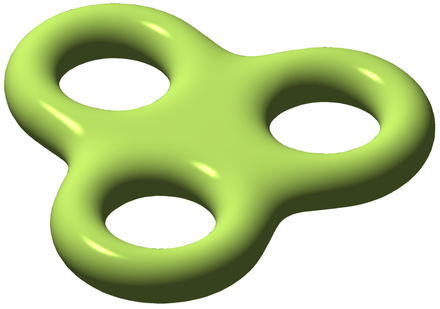
\includegraphics[scale = 1]{RiemannSurface}
**** Riemann Surface of genus 3, from Wikimedia ****

Of course this definition does not apply to curves over fields other than $\CC$, and doesn't relate the genus to the algebra of the curve. However, we can relate the topological genus of a curve directly to its topological Euler characteristic
$
\chi_{top}(C) = 2-2g.
$
By the Hopf index theorem, the topological Euler characteristic is the degree of the tangent sheaf, or equivalently, minus the degree of the cotangent sheaf $\omega_{C}$; that is, $\deg K_{C} = 2g-2$, and thus

$$
g(C) = \frac{\deg(K_C)}{2} + 1.
$$
(This formula serves to define the genus of a smooth projective curve over any field).

Other characterizations of the genus require more machinery to establish. We will give some here, and use  tools from the following section to prove equivalence.

\begin{enumerate}

\item\label{genus 1forms} $g(C)$ is the dimension of the vector space of regular 1-forms (that is, global sections of the
cotangent sheaf) on $C$.

\item The (Zariski) Euler characteristic of the structure sheaf of $C$ is $\chi(\cO_C) = h^0(\cO_C) - h^1(\cO_C)$. Since $h^0(\cO_C) = 1$, 
$$
g(C) = 1 - \chi(\cO_C).
$$

Recall that if $X\subset \PP^{r} = \PP(V)$ is any projective scheme, the \emph{homogeneous coordinate ring} of $X$
is the ring $S/I(X)$ where $S = \Sym V \cong \CC[x_{0}, \dots, x_{r}]$ and $I(V)\subset S$ is the ideal of homogeneous
forms that vanish on $X$.

\item\label{genus Hilbert} Suppose that $C \subset \PP^r = \PP(V)$ is a smooth curve of degree $d$  with homogeneous coordinate ring
$S_C$, then the function $d \mapsto \dim_\CC (S_C)_d$ is equal to a polynomial function $p_C(m)$ for large $d$. We have:
$$
p_C(m) =  dm - g + 1,
$$
so $g(C) = 1 - p_C(0)$. 
\end{enumerate}

\subsection{The Riemann-Roch Theorem}

To prove that these formulas for the genus are correct, we use \trr and Serre duality (sometimes called Kodaira-Serre duality, since Kodaira was responsible for the analytic version.)

\begin{theorem}[Riemann-Roch Theorem]\label{RR}
 If $C$ is a smooth, connected projective curve of genus $g$, and $D$ a divisor of degree $d$ on $C$ then
$$
h^0(D) = d - g + 1 + h^0(K_C - D).
$$
\end{theorem}

For example, if we take $D=0$, this tells us that $h^0(K) = g$, proving the characterization~(\ref{genus 1forms}) above. Also, since $h^0(D) = 0$ for any divisor $D$ of negative degree, the formula gives the dimension of $h^{0}(D)$ when $\deg D$ is large:

\begin{corollary}\label{nonspecial RR}
For any divisor of degree $d \geq 2g-1$, we have
$$
h^0(D) = d - g + 1.
$$
\end{corollary}

Using this, we can apply Proposition~\ref{very ample} to show that all high degree divisors come from embeddings:

\begin{corollary}\label{degree 2g+1 embedding}
Let $D$ be a divisor of degree $d$ on a smooth, connected projective curve of genus $g$. If $d \geq 2g$, the complete linear series $|D|$ is base point free; and if $d \geq 2g+1$ the associated morphism $\phi_D : C \to \PP^{d-g}$ is an embedding, so that
$D$ is the preimage of the intersection of $C$ with a hyperplane in $ \PP^{d-g}$.
\end{corollary}

Since the complement of a hyperplane in projective space is an affine space, we get an affine embedding result too:

\begin{corollary}
 If $C$ is any smooth, connected projective curve and $\emptyset \neq \Gamma \subset C$ a finite subset then $C \setminus \Gamma$ is affine.
\end{corollary}
\begin{proof}
Let $D$ be the divisor defined by $\Gamma$ By Corollary~\ref{degree 2g+1 embedding} a high multiple of $D$ is very ample,
and gives an embedding $\phi: C\to \PP^n$ such that the preimage of the intersection of $C$ with some hyperplane $H$
is a multiple of $D$. It follows that $C\setminus \Gamma$ is embedded in $\PP^n\setminus H$.
\end{proof}


We can  use \TRR in the simple case of Corollary~\ref{nonspecial RR} to determine the Hilbert polynomial of a projective curve. To do this, let $C \subset \PP^r$ be a smooth curve of degree $d$ and genus $g$, and consider the exact sequence of sheaves
$$
0 \rTo \cI_{C/\PP^r}(m) \rTo \cO_{\PP^r}(m) \rTo \cO_C(m) \rTo 0
$$
and the corresponding exact sequence
$$
 H^0(\cO_{\PP^r}(m)) \rTo^{\rho_m} H^0(\cO_C(m)) \rTo H^1(\cI_{C/\PP^r}(m)) \rTo 0.
$$

The \emph{Hilbert function} $h_C$ of $C$  is defined by
$$
h_C(m) = \dim_{\CC} (S_{C})_{m} = \rank(\rho_m).
$$
By Theorem~\ref{Serre vanishing} we have $H^1(\cI_{C/\PP^r}(m)) = 0$ for large $m$, so $h_{C}(m) = h^0(\cO_C(m))$, for large $m$, which, by \trr, equals $md-g+1$, again for large $m$. Thus, the Hilbert polynomial of $C \subset \PP^r$ is $p_C(m) = dm-g+1$, establishing the characterization~(\ref{genus Hilbert}).
 
The Riemann-Roch formula does \emph{not} give us a formula for the dimension $h^0(D)$ when $h^0(K_C - D)>0$; such divisors $D$ are called \emph{special divisors}, or \emph{special divisor classes}. The existence or non-existence of divisors $D$ with given $h^{0}(D)$ and $h^{1}(D)$ often serves to distinguish one curve from another, and will be an important part of our study.
 
 
\begin{fact}
 Classically, the dimension $h^0(K_C-D) = h^1(D)$ was called the \emph{superabundance} of $D$: the idea was that a divisor of degree $d$ had, at a minimum, $d-g+1$ sections and $h^1(D)$ represented the number of ``extra" sections. Even though the introduction of cohomology was still almost a century away, the ranks of cohomology groups $h^1$ had classical names, often involving the term superabundance---a premonition of the Riemann-Roch theorem in general.
\end{fact}
 
\begin{fact}
If $k$ is a field that is not algebraically closed there may be genus 0 curves that are not isomorphic to $\PP^1$. However, they must be``forms'' of $\PP^1$ in the sense that they become isomorphic to $\PP^1$ after extension of scalars to 
the algebraic closure $\overline k$ of $k$. The unique example with $k = \RR$ is the conic $x^2+y^2+z^2 = 0$. Indeed, any form of $\PP^1$ over any field $k$ can all be embedded in $\PP_{k}^2$ (by using the anti-canonical linear system.

The curve $\PP_k^1$ itself may be described as the scheme of left ideals of $k$-vector-space dimension 1 in the ring of
$2\times 2$ matrices over $k$ (such an ideal can be embedded in the matrix ring as a linear combination of the 2 columns in an appropriate sense). More generally, any scheme that is a form of $\PP^1$ over $k$
may be described as the scheme of 1-dimensional left ideals in a central simple ($=$ Azumaya) algebra over $k$---though as a set this scheme has no $k$-rational points unless the algebra is the algebra of $2\times 2$ matrices!
\end{fact}
\subsection{Serre duality}

In general, if $\cF$ and $\cG$ are coherent sheaves on a scheme $X$, we have for every $i$ and $j$ a cup product map
$$
H^i(\cF) \otimes H^j(\cG) \to H^{i+j}(\cF \otimes \cG).
$$

\begin{theorem}[Serre Duality]\label{sd} Let $C$ be a smooth connected projective curves with canonical divisor $K$. We have
 $$
h^1(K) = 1
$$
and the cup product map
$$
H^1(D) \otimes H^0(K-D) \to H^1(K)
$$
is a perfect pairing; that is, it induces a natural isomorphism
$$
H^1(D) = H^0(K-D)^*.
$$
\end{theorem}

\subsection{A partial proof}

Combining \TRR and Serre Duality we get:
\begin{corollary}
 If $C$ is a smooth, connected projective curve and $D$ is a divisor on $C$ then
\end{corollary}
$$
\chi(\sO_C(C)) := h^0(D) - h^1(D) = d-g+1
$$
or in other words, for any invertible sheaf $\cL$ of degree $d$ on $C$,
$$
\chi(\cL) = d-g+1
$$
which is pretty easy to prove. To see this, observe that for any invertible sheaf $\cL$ on $C$ and any point $p \in C$ we have an exact sequence of sheaves
$$
0 \to \cL(-p) \to \cL \to \cL_p \to 0.
$$
It follows that $\chi(\cL(-p)) = \chi(\cL) - 1$, so that Riemann-Roch for $\cL$ is equivalent to Riemann-Roch for $\cL(-p)$. Since any divisor can be obtained from 0 by adding and subtracting points, the Riemann-Roch formula for an arbitrary $\cL$ follows from the special case $\cL = \cO_C$.

\subsection{Clifford's theorem}

\begin{theorem}\label{Clifford}
Let $C$ be a curve of genus $g$ and $\cL$ a line bundle of degree $d \leq 2g-2$. Then
$$
r(\cL) \leq \frac{d}{2}.
$$
Moreover, if  equality holds then we must have either
\begin{enumerate}
\item $d=0$ and $\cL = \cO_C$;
\item $d = 2g-2$ and $\cL = K_C$; or
\item $C$ is hyperelliptic, and $|\cL|$ is a multiple of the $g^1_2$ on $C$.
\end{enumerate}
\end{theorem}

\begin{proof}
The proof of Clifford rests on a very basic construction and observation. 

To start, let $\cD = (\cL,V)$ and $\cE = (\cM, W)$ be two linear series on a curve $C$. By the \emph{sum} $\cD + \cE$ of $\cD$ and $\cE$, we will mean the pair 
$$
\cD + \cE = (\cL \otimes \cM, U) 
$$
where $U \subset H^0(\cL \otimes \cM)$ is the subspace generated by the image of $V \otimes W$, under the multiplication/cup product map $H^0(\cL) \otimes H^0(\cM) \to H^0(\cL \otimes \cM)$---in other words, it's the subspace of the complete linear series $|\cL\otimes \cM|$ spanned by divisors of the form $D+E$, with $D \in \cD$ and $E \in \cE$.

The observation is a simple one:
\begin{lemma}
If $\cD$ and $\cE$ are two nonempty linear series on a curve $C$, then
$$
\dim(\cD + \cE) \geq \dim \cD + \dim \cE.
$$
\end{lemma}
(To see this, we observe that to say $\dim \cD \geq m$ means exactly that we can find a divisor $D \in \cD$ containing any given $m$ points of $C$; since $\cD + \cE$ contains all pairwise sums $D + E$ with $D \in \cD$ and $E \in \cE$, we can certainly find a divisor $F \in cD + \cE$ containing any given $\dim \cD + \dim \cE$ points of $C$.)

Given this lemma, the proof of Clifford follows simply by applying it to the pair $|\cL|$ and $|K_C\otimes \cL^{-1}|$: by Riemann-Roch, we have
$$
r(K_C\otimes \cL^{-1}) = r(\cL) +g - d - 1
$$
and so we deduce that
$$
g = r(K_C) + 1 \geq r(\cL) + r(K_C\otimes \cL^{-1}) + 1 \geq 2r(\cL) +g - d;
$$
hence $r(\cL) \leq d/2$.

Our proof of the second half of Clifford rests on a basic fact about the geometry of hyperplane sections of a curve in projective space (Proposition~\ref{monodromy of hyperplane section}); we'll defer it until we've established that fact.
\end{proof}



\section{The canonical morphism}

Given the central role played by the canonical divisor class, it is natural to look at the geometry of the morphism $\phi_K : C \to \PP^{g-1}$ associated to the complete canonical series $|K|$.  By the Riemann-Roch theorem, 
$h^{0}(K) = g(C)$, so $|K|$ cannot define a non-constant morphism unless $g(C)\geq 2$, and cannot define an embedding unless $g(C)\geq 3$.

\begin{definition}
A curve $C$ of genus $g \geq 2$ is said to be \emph{hyperelliptic} if there exists a morphism $f: C \to \PP^1$ of degree 2. \end{definition}

%equivalently, if there exists a invertible sheaf $\cL$ on $C$ of degree 2 with $h^0(\cL) = 2$.

\begin{proposition}
The canonical morphism $\phi_K : C \to \PP^{g-1}$ is an embedding if and only if $C$ is not hyperelliptic.
\end{proposition}

\begin{proof}
By Corollary~\ref{degree 2g+1 embedding} we have to show that for any pair of points $p, q \in C$ we have
$$
h^0(K_C(-p-q)) = h^0(K_C)-2 = g-2.
$$
Applying \trr we see that this would fail if and only if $h^0(\cO_C(p+q)) \geq 2$ for some $p,q \in C$, and by Lemma~\ref{deg 2 morphism} $|p+q|$ would define a degree 2 morphism to $\PP^{1}$. 
\end{proof}

\begin{lemma}\label{deg 2 morphism}
Let $C$ be a smooth, projective curve of genus $g\geq 2$. Any invertible sheaf of degree 2 on $C$ defines a morphism to $\PP^{1}$. In particular, if $g(C) = 2$ then the canonical series $|K_{C}|$ defines a 2 to 1 morphism to $\PP^{1}$.
\end{lemma}

\begin{proof}
 If this happens,
we claim that $\cO_C(p+q)$ is basepoint free, so that $C$ is hyperelliptic. To finish the proof, by Corollary~\ref{degree 2g+1 embedding} it suffices to show that
 an invertible sheaf $\sL$ of degree 1 on $C$ must have $h^{0}(\sL)\leq 1$.
 
Suppose that $\sigma_{0}, \sigma_{1}$ were two linearly independent sections of $\sL$. Each $\sigma_{i}$ vanishes at a unique point $p_{i}$. If $p_{0}= p_{1}$ then a linear combination of $\sigma_{0}, \sigma_{1}$ would be a section vanishing to order $\geq 2$, which is impossible, so $\sL$ is basepoint free, and defines a degree 1 morphism $C\to \PP^{1}$. Such a morphism must be an isomorphism (because $\PP^{1}$ is normal), contradicting $g(C) \geq 2$.
\end{proof}

\fix{the following argument is only set-theoretic. Admit this or make it precise}
Note that if $C$ is hyperelliptic, the morphism $\phi_K$ factors through the degree 2 morphism $\pi : C \to \PP^1$: if $\{p,q\} \subset C$ is a fiber of this morphism, we have $h^0(\cO_C(p+q)) = 2$ and hence $\phi_K(p) = \phi_K(q)$. The image of the morphism $\phi_K$ is a nondegenerate curve of degree $g-1$ in $\PP^{g-1}$, which we will see is a \emph{rational normal curve}. This observation implies in particular that if $C$ is hyperelliptic of genus $g \geq 2$, then the invertible sheaf $\cL$ of degree 2 with $h^0(\cL) = 2$ is in fact unique.

Among curves with $g \geq 3$ the hyperelliptic curves are very special: in the family of all curves, as we'll see, they comprise a closed subvariety. Also, the behavior of linear series and morphisms on a hyperelliptic curve is very different from that of series on a general curve; when we discuss the geometry of curves of low genus in the Chapter~\ref{}, we will exclude  the hyperelliptic case, and deal with this case in a separate chapter.

For non-hyperelliptic curves, however, the geometry of the canonical morphism, and its image, the canonical curve, are the keys to understanding the curve. We'll see this in detail in many cases in the following chapter; for now, we mention one highly useful result along these lines.

\fix{add here: canonical series on plane curves cut by $|\cO_{\PP^2}(d-3)|$; consequence that no smooth plane curve can be hyperelliptic}

\fix{maybe move initial discussion of hyperelliptic curves from Ch. 6 to a section here}

\fix{maybe add to this chapter: differentials on plane curves $C$, possibly with nodes or more general singularities; adjoint conditions; algorithm for determining the complete linear system associated to a divisor $D$ on $C$}

\subsection{The geometric Riemann-Roch theorem}

Let's state this first in a relatively simple case: let $C$ be a nonhyperelliptic curve, embedded in $\PP^{g-1}$ by its canonical series and let $D = p_1+\dots + p_d$ be a divisor consisting of $d$ distinct points; let $\overline D$ be the span of the points $p_i \in C \subset \PP^{g-1}$. Since the hyperplanes in $\PP^{g-1}$ containing $\{p_1,\dots,p_d\}$ correspond (up to scalars) to sections of $K_C$ vanishing at all the points $p_i$, we see that
$$
h^0(K_C-D) = g - 1 - \dim \overline D.
$$
Plugging this into the Riemann-Roch formula, we arrive at the statement
$$
r(D) = d - 1 - \dim \overline D;
$$
or in other words, \emph{the dimension of the linear series $|D|$ in which the divisor $D$ moves is equal to the number of linear relations on the points $p_i$ on the canonical curve}. Thus, for example, if $D = p_1+p_2+p_3$, we see that $D$ moves in a pencil if and only if the points $p_i$ are collinear.

We can extend this statement to the case of arbitrary effective divisors $D$ (and even hyperelliptic curves) if we define our terms correctly. To do this, suppose $f : C \to \PP^d$ is any morphism, and $D \subset C$ any divisor. We define the \emph{span} of  $f(D)$ to be the intersection
$$
\overline{f(D)} = \bigcap_{H \mid f^{-1}(H)\supset D} H 
$$
of all hyperplanes in $\PP^d$ whose preimage in $C$ contains $D$. 

\begin{theorem}[Geometric Riemann-Roch Theorem]\label{geometric RR}
If $C$ is any curve of genus $g \geq 2$,  $\phi : C \to \PP^{g-1}$ its canonical morphism and $D \subset C$ any effective divisor of degree $d$, then
$$
r(D) = d - 1 - \dim \overline{\phi(D)}.
$$
\end{theorem}
 

\input footer.tex
%header and footer for separate chapter files

\ifx\whole\undefined
\documentclass[12pt, leqno]{book}
\usepackage{graphicx}
\input style-for-curves.sty
\usepackage{hyperref}
\usepackage{showkeys} %This shows the labels.
%\usepackage{SLAG,msribib,local}
%\usepackage{amsmath,amscd,amsthm,amssymb,amsxtra,latexsym,epsfig,epic,graphics}
%\usepackage[matrix,arrow,curve]{xy}
%\usepackage{graphicx}
%\usepackage{diagrams}
%
%%\usepackage{amsrefs}
%%%%%%%%%%%%%%%%%%%%%%%%%%%%%%%%%%%%%%%%%%
%%\textwidth16cm
%%\textheight20cm
%%\topmargin-2cm
%\oddsidemargin.8cm
%\evensidemargin1cm
%
%%%%%%Definitions
%\input preamble.tex
%\input style-for-curves.sty
%\def\TU{{\bf U}}
%\def\AA{{\mathbb A}}
%\def\BB{{\mathbb B}}
%\def\CC{{\mathbb C}}
%\def\QQ{{\mathbb Q}}
%\def\RR{{\mathbb R}}
%\def\facet{{\bf facet}}
%\def\image{{\rm image}}
%\def\cE{{\cal E}}
%\def\cF{{\cal F}}
%\def\cG{{\cal G}}
%\def\cH{{\cal H}}
%\def\cHom{{{\cal H}om}}
%\def\h{{\rm h}}
% \def\bs{{Boij-S\"oderberg{} }}
%
%\makeatletter
%\def\Ddots{\mathinner{\mkern1mu\raise\p@
%\vbox{\kern7\p@\hbox{.}}\mkern2mu
%\raise4\p@\hbox{.}\mkern2mu\raise7\p@\hbox{.}\mkern1mu}}
%\makeatother

%%
%\pagestyle{myheadings}

%\input style-for-curves.tex
%\documentclass{cambridge7A}
%\usepackage{hatcher_revised} 
%\usepackage{3264}
   
\errorcontextlines=1000
%\usepackage{makeidx}
\let\see\relax
\usepackage{makeidx}
\makeindex
% \index{word} in the doc; \index{variety!algebraic} gives variety, algebraic
% PUT a % after each \index{***}

\overfullrule=5pt
\catcode`\@\active
\def@{\mskip1.5mu} %produce a small space in math with an @

\title{Personalities of Curves}
\author{\copyright David Eisenbud and Joe Harris}
%%\includeonly{%
%0-intro,01-ChowRingDogma,02-FirstExamples,03-Grassmannians,04-GeneralGrassmannians
%,05-VectorBundlesAndChernClasses,06-LinesOnHypersurfaces,07-SingularElementsOfLinearSeries,
%08-ParameterSpaces,
%bib
%}

\date{\today}
%%\date{}
%\title{Curves}
%%{\normalsize ***Preliminary Version***}} 
%\author{David Eisenbud and Joe Harris }
%
%\begin{document}

\begin{document}
\maketitle

\pagenumbering{roman}
\setcounter{page}{5}
%\begin{5}
%\end{5}
\pagenumbering{arabic}
\tableofcontents
\fi

%\documentclass[12pt, leqno]{book}
%\usepackage{amsmath,amscd,amsthm,amssymb,amsxtra,latexsym,epsfig,epic,graphics}
%\usepackage[matrix,arrow,curve]{xy}
%\usepackage{graphicx}
%\usepackage{diagrams}
%%\usepackage{amsrefs}
%%%%%%%%%%%%%%%%%%%%%%%%%%%%%%%%%%%%%%%%%%
%%\textwidth16cm
%%\textheight20cm
%%\topmargin-2cm
%\oddsidemargin.8cm
%\evensidemargin1cm
%
%%%%%%Definitions
%\input preamble.tex
%\def\TU{{\bf U}}
%\def\AA{{\mathbb A}}
%\def\BB{{\mathbb B}}
%\def\CC{{\mathbb C}}
%\def\QQ{{\mathbb Q}}
%\def\RR{{\mathbb R}}
%\def\facet{{\bf facet}}
%\def\image{{\rm image}}
%\def\cE{{\cal E}}
%\def\cF{{\cal F}}
%\def\cG{{\cal G}}
%\def\cH{{\cal H}}
%\def\cHom{{{\cal H}om}}
%\def\h{{\rm h}}
% \def\bs{{Boij-S\"oderberg{} }}
%
%\makeatletter
%\def\Ddots{\mathinner{\mkern1mu\raise\p@
%\vbox{\kern7\p@\hbox{.}}\mkern2mu
%\raise4\p@\hbox{.}\mkern2mu\raise7\p@\hbox{.}\mkern1mu}}
%\makeatother
%
%%%
%%\pagestyle{myheadings}
%\date{April 30, 2018}
%%\date{}
%\title{Curves}
%%{\normalsize ***Preliminary Version***}} 
%\author{David Eisenbud and Joe Harris }
%
%\begin{document}

\chapter{Brill-Noether Theory}



\section{What linear series exist?}

In the last chapter, we established a basic correspondence between maps of curves to projective space and linear systems. The next question to ask, naturally, is ``What linear systems exist?"

There are various ways to interpret this question. Let's start by taking the question in its plain, unvarnished form---for which $g, r$ and $d$ does there exist a curve $C$ of genus $g$ and a linear system $(\cL,V)$ on $C$ of degree $d$ and dimension $r$? In this form, the answer is given for line bundles of large degree $d \geq 2g-1$ by the Riemann-Roch theorem: on any curve, there exists a linear series of degree $d \geq 2g-1$ and dimension $r$ iff $r \leq d-g$. 

\subsection{Clifford's theorem} 

Riemann-Roch still leaves open the question of what linear systems of degree $d \leq 2g-2$ may exist on a curve of genus $g$. The answer is given by the classical theorem of Clifford:

\begin{theorem}\label{Clifford}
Let $C$ be a curve of genus $g$ and $\cL$ a line bundle of degree $d \leq 2g-2$. Then
$$
r(\cL) \leq \frac{d}{2}.
$$
Moreover, if  equality holds then we must have either
\begin{enumerate}
\item $d=0$ and $\cL = \cO_C$;
\item $d = 2g-2$ and $\cL = K_C$; or
\item $C$ is hyperelliptic, and $|\cL|$ is a multiple of the $g^1_2$ on $C$.
\end{enumerate}
\end{theorem}

\begin{proof}

\end{proof}

Combining this with Riemann-Roch, we arrive at the

\begin{theorem}\label{arbitrary linear series}
There exists a curve $C$ of genus $g$ and line bundle $\cL$ of degree $d$ on $C$ with $h^0(\cL) \geq r+1$ if and only if
$$
r \leq
\begin{cases}
d-g, \quad \text{if } d \geq 2g-1; \text{ and} \\
d/2,  \quad \text{if } 0 \leq d \leq 2g-2.
\end{cases}
$$
\end{theorem}

\subsection{Castelnuovo's theorem}

Theorem~\ref{arbitrary linear series} gives a complete and sharp answer to the question originally posed: for which $d,r$ and $g$ does there exists a triple $(C,\cL,V)$ with $C$ a curve of genus $g$, $\cL$ a line bundle of degree $d$ on $C$ and $V \subset H^0(\cL)$ of dimension $r+1$. 

But maybe that wasn't the question we meant to ask! After all, we're interested in describing curves in projective space as images of abstract curves $C$ under maps given by linear systems on $C$. Observing that the linear series that achieve equality in Clifford's theorem give maps to $\PP^r$ that are 2 to 1 onto a rational curve, we might hope that we would have a different---and more meaningful---answer if we  restrict our attention to linear series $\cD = (\cL,V)$ for which the associated map $\phi_\cD$ is at least a birational embedding.  With this restriction, the question is tantamount to the

\begin{question}
What is the largest possible genus of an irreducible, nondegenerate curve $C \subset \PP^r$ of degree $d$?
\end{question}

The answer to this question is indeed quite different from the inequality provided by Theorem~\ref{arbitrary linear series}. It is the content of \emph{Castelnuovo's theorem}, which gives a sharp answer to this question. We'll sketch the derivation of the inequality here; we'll prove that it is in fact sharp and describe in detail  the curves that achieve it in Chapter~\ref{}.

To start, Castelnuovo's bound follows from a very straightforward approach: if $C$ is a curve of degree $d$ and genus $g$ in $\PP^r$, the idea is to prove successive lower bounds for the dimensions $h^0(\cO_C(m))$ of multiples of the $g^r_d$ cut on $C$ by hyperplanes. For large values of $m$, of course, the line bundle $\cO_C(m)$ is non-special, and so a lower bound on the dimension of its space of sections translates, via Riemann-Roch, into an upper bound on the genus $g$.

\begin{definition}
Let $\cL$ be any line bundle on a smooth projective variety $X$, and $D = \{p_1,\dots,p_d\}$ a collection of points of $X$. By the \emph{number of conditions imposed by $D$ on sections of $\cL$} we will mean simply the difference
$$
h^0(\cL) - h^0(\cL \otimes \cI_{D/X});
$$
that is, the codimension in $H^0(\cL)$ of the subspace of sections vanishing on $D$. More generally, if $V \subset H^0(\cL)$ is any linear system, by the number of conditions imposed by $D$ on $V$ we will mean the difference
$$
\dim(V) - \dim \left(V \cap H^0(\cL\otimes \cI_{D/X}) \right).
$$
\end{definition}
Thus, for example, if $X = \PP^r$, the number of conditions imposed by $D$ on $H^0(\cO_{\PP^r}(m))$ is the value $h_D(m)$ of the Hilbert function of $D$.
Note that the number of conditions imposed by $D$ on a linear system $V$ is necessarily less than or equal to the degree $d$ of $D$; if it is equal we say that $D$ \emph{imposes independent conditions on $V$}.

To apply this notion, suppose $C \subset \PP^r$ is an irreducible, nondegenerate curve. Let $\Gamma = C \cap H$ be a general hyperplane section of $C$. Let $V_m \subset H^0(\cO_C(m))$ be the linear series cut on $C$ by hypersurfaces of degree $m$ in $\PP^r$, that is, the image of the restriction map
$$
H^0(\cO_{\PP^r}(m)) \to H^0(\cO_C(m)).
$$
We have then a series of more or less trivial inequalities:
\begin{align*}
h^0(\cO_C(m)) - h^0(\cO_C(m-1)) & \geq \text{\# of conditions imposed by $\Gamma$ on $H^0(\cO_C(m))$} \\
&\geq \text{\# of conditions imposed by $\Gamma$ on $V_m$} \\
&\geq \text{\# of conditions imposed by $\Gamma$ on $H^0(\cO_{\PP^r}(m))$} ;
\end{align*}
in other words, the dimension $h^0(\cO_C(m))$ is bounded below by the sum
$$
h^0(\cO_C(m)) \geq \sum_{k=0}^m h_\Gamma(k).
$$

We need, in other words, a lower bound on the Hilbert function of a general hyperplane section $\Gamma$ of our curve $C$. This is turn requires that we have some knowledge of the geometry of $\Gamma$, but not in fact all that much: all we need is the basic

\begin{lemma}[general position lemma]
If $C \subset \PP^r$ is an irreducible, nondegenerate curve and $\Gamma = C \cap H$ a general hyperplane section of $C$, then the points of $\Gamma$ are in linear general position in $H \cong \PP^{r-1}$, meaning no $r$ points of $\Gamma$ lie in a hyperplane $\PP^{r-2} \subset H$.
\end{lemma}
Thus, for example, if $C \subset \PP^3$ is a space curve, no three points of $\Gamma = H \cap C$ will be colinear.

\begin{exercise}
Prove this directly.
\end{exercise}

The general position lemma was originally asserted by Castelnuovo. In more modern treatments, it is usually deduced as a special case of the more general

\begin{lemma}[uniform position lemma]
With $C \subset \PP^r$ and $\Gamma = C \cap H$ as above, any two subsets $\Gamma', \Gamma'' \subset \Gamma$ of the same cardinality have the same Hilbert function, i.e., impose the same number of conditions on $\cO_{\PP^{r-1}}(m)$ for all $m$.
\end{lemma}

The general position lemma is just the special case $m=1$ of the uniform position lemma. This may not seem like much information about $\Gamma$, but in fact it's all we need to prove a sharp bound! The basic (and completely elementary) statement is

\begin{proposition}
If $\Gamma \subset \PP^n$ is a collection of $d$ points in linear general position and spanning $\PP^n$, then 
$$
h_\Gamma(m) \geq \min\{d, mn+1\}
$$
\end{proposition}

\begin{proof}
Suppose first that $d \geq mn+1$, and let $p_1,\dots,p_{mn+1} \in \Gamma$ be any subset of $mn+1$ points. We want to show that $\Gamma' = \{p_1,\dots,p_{mn+1}\}$ imposes independent conditions of $H^0(\cO_{\PP^n}(m))$, that is, for any $p_i \in \Gamma'$ we can find a hypersurface $X \subset \PP^n$ of degree $m$ containing all the points $p_1,\dots, \hat{p_i},\dots,p_{mn+1}$ but not containing $p_i$.

This is easy: simply group the $mn$ points of $\Gamma' \setminus \{p_i\}$ into $m$ subsets $\Gamma_k$ of cardinality $n$; each set $\Gamma_k$ will span a hyperplane $H_k \subset \PP^n$, and we can take $X = H_1 \cup \dots \cup H_m$. 
\end{proof}

This may seem like a crude argument, but the bound derived is sharp: any collection of point $\Gamma \subset \PP^n$ lying on a rational normal curve $D \subset \PP^n$ has exactly this Hilbert function.

At this point, all that remains is to add up the lower bounds in the proposition. To this end, let $C \subset \PP^r$ be as above an irreducible, nondegenerate curve of degree $d$, and set $M = \lfloor{\frac{d-1}{r-1}}\rfloor$, so that we can write
$$
d = M(r-1) + 1 + \epsilon \quad \text{ with } \quad 0 \leq \epsilon \leq r-2.
$$
We have then
\begin{align*}
h^0(\cO_C(M)) &\geq \sum_{k=0}^M h^0(\cO_C(k)) - h^0(\cO_C(k-1)) \\
&\geq  \sum_{k=0}^M k(r-1)+1 \\
&= \frac{M(M+1)}{2}(r-1) + M + 1
\end{align*}
and similarly
$$
h^0(\cO_C(M+m)) \geq \frac{M(M+1)}{2}(r-1) + M + 1 + md.
$$
For sufficiently large $m$, the line bundle $\cO_C(M+m)$ will be nonspecial, so we can plug this in to Riemann-Roch to arrive at
\begin{align*}
g &= (M+m)d - h^0(\cO_C(M+m)) + 1 \\
&\leq (M+m)d - \bigl(  \frac{M(M+1)}{2}(r-1) + M + 1 + md \bigr) \\
& = M\bigl( M(r-1) + 1 + \epsilon \bigr) - \bigl(  \frac{M(M+1)}{2}(r-1) + M + 1 \bigr) \\
&= \frac{M(M-1)}{2}(r-1) + M\epsilon.
\end{align*}

To summarize our discussion: for positive integers $d$ and $r$, we write
$$
 d = M(r-1) + 1 + \epsilon \quad \text{ with } \quad 0 \leq \epsilon \leq r-2
$$
and set
$$
\pi(d,r) = \frac{M(M-1)}{2}(r-1) + M\epsilon.
$$
In these terms, we have proved the

\begin{theorem}[Castelnuovo's bound]
If $C \subset \PP^r$ is an irreducible, nondegenerate curve of degree $d$ and genus $g$, then
$$
g \leq \pi(d,r).
$$
\end{theorem}

We will see in Chapter~\ref{} that this is in fact sharp: for every $r$ and $d \geq r$, there do exist such curves with genus exactly $\pi(d,r)$. For now, we make a few observations:

\begin{enumerate}
\item In case $r=2$, all the inequalities used in the derivation of Castenuovo's bound are in fact equalities, and indeed we see that in this case $\pi(d,2) = \binom{d-1}{2}$ is the genus of a smooth plane curve of degree $d$.

\item In case $r=3$, we have
$$
\pi(d,3) =
\begin{cases}
\left( k - 1 \right)^2 &\text{ if $d=2k$ is even; and} \\
k(k-1) &\text{ if $d=2k+1$ is odd.}
\end{cases}
$$
In this case again, it's not hard to see the bound is sharp: these are exactly the genera of curves of bidegree $(k,k)$ and $(k+1,k)$ on a quadric surface $Q \cong \PP^1 \times \PP^1 \subset \PP^3$.
\item In general, we see that for fixed $r$ asymptotically
$$
\pi(d,r) \sim \frac{d^2}{2(r-1)}.
$$
\end{enumerate}


\begin{exercise}
Show that with $C$ as above, the line bundle $\cO_C(M)$ is nonspecial. (We will see in Section~\ref{} that this is sharp; that is, there exist such curves $C$ with $\cO_C(M-1)$ special).
\end{exercise}

\section{Brill-Noether theory}

\subsection{Basic questions addressed by Brill-Noether theory}

\subsection{Heuristic argument leading to the statement of BN}

The Brill-Noether theorem, as we'll see, is a far-reaching description of the linear series to be found on a general curve. It starts, though, with a relatively simple dimension count---one that was first carried out almost a century and a half ago.

To set this up, let $C$ be a smooth projective curve of genus $g$, and $D = p_1 + \dots + p_d$ a divisor on $C$. We'll assume here the points $p_i$ are distinct; the same argument (albeit with much more complicated notation) can be carried out in general.

When does the divisor $D$ move in an $r$-dimensional linear series? Riemann-Roch gives an answer: it says that $h^0(D) \geq r+1$ if and only if the vector space $H^0(K-D)$ of 1-forms vanishing on $D$ has dimension at least $g-d+r$---that is, if and only if the rank of the evaluation map
$$
H^0(K) \to H^0(K|_D) = \oplus K_{p_i}
$$
has rank at most $d-r$. 

We can represent this map by a $g \times d$ matrix. Choose a basis $\omega_1,\dots,\omega_g$ for the space $H^0(K)$ of 1-forms on $C$; choose an analytic open neighborhood $U_j$ of each point $p_j \in D$ and choose a local coordinate $z_j$ in $U_j$ around each point $p_j$, and write
$$
\omega_i = f_{i,j}(z_j)dz_j
$$
in $U_j$. We will have $r(D) \geq r$ if and only if the  matrix-valued function
$$
A(z_1,\dots,z_d) = 
\begin{pmatrix}
f_{1,1}(z_1) & f_{2,1}(z_1) & \dots & f_{g,1}(z_1) \\
f_{1,2}(z_2) & f_{2,2}(z_2) & \dots & f_{g,2}(z_2) \\
\vdots & \vdots &  & \vdots \\
f_{1,d}(z_d) & f_{2,d}(z_d) & \dots & f_{g,d} (z_d)
\end{pmatrix}
$$
has rank $d-r$ or less at $(z_1,\dots,z_d) = (0,\dots,0)$.

The point is, we can think of $A$ as a matrix valued function in the open set $U = U_1 \times U_2 \times \dots \times U_d \subset C_d$; and for divisors $D \in U$, we have $r(D) \geq r$ if and only if $\rank(A(D)) \leq d-r$. Now, in the space $M_d,g$ of $d \times g$ matrices, the subset of matrices of rank $d-r$ or less has codimension $r(g-d+r)$, and so we might naively expect that the locus of divisors with $r(D) \geq r$ would have dimension $d - r(g-d+r)$

\section{Statement of BN and add-ons}

 (very ampleness if $r \geq 3$, irreducibility of $W^r_d$ when $\rho > 0$, etc.)

\section{Special cases and consequences}


\input footer.tex
%header and footer for separate chapter files

\ifx\whole\undefined
\documentclass[12pt, leqno]{book}
\usepackage{graphicx}
\input style-for-curves.sty
\usepackage{hyperref}
\usepackage{showkeys} %This shows the labels.
%\usepackage{SLAG,msribib,local}
%\usepackage{amsmath,amscd,amsthm,amssymb,amsxtra,latexsym,epsfig,epic,graphics}
%\usepackage[matrix,arrow,curve]{xy}
%\usepackage{graphicx}
%\usepackage{diagrams}
%
%%\usepackage{amsrefs}
%%%%%%%%%%%%%%%%%%%%%%%%%%%%%%%%%%%%%%%%%%
%%\textwidth16cm
%%\textheight20cm
%%\topmargin-2cm
%\oddsidemargin.8cm
%\evensidemargin1cm
%
%%%%%%Definitions
%\input preamble.tex
%\input style-for-curves.sty
%\def\TU{{\bf U}}
%\def\AA{{\mathbb A}}
%\def\BB{{\mathbb B}}
%\def\CC{{\mathbb C}}
%\def\QQ{{\mathbb Q}}
%\def\RR{{\mathbb R}}
%\def\facet{{\bf facet}}
%\def\image{{\rm image}}
%\def\cE{{\cal E}}
%\def\cF{{\cal F}}
%\def\cG{{\cal G}}
%\def\cH{{\cal H}}
%\def\cHom{{{\cal H}om}}
%\def\h{{\rm h}}
% \def\bs{{Boij-S\"oderberg{} }}
%
%\makeatletter
%\def\Ddots{\mathinner{\mkern1mu\raise\p@
%\vbox{\kern7\p@\hbox{.}}\mkern2mu
%\raise4\p@\hbox{.}\mkern2mu\raise7\p@\hbox{.}\mkern1mu}}
%\makeatother

%%
%\pagestyle{myheadings}

%\input style-for-curves.tex
%\documentclass{cambridge7A}
%\usepackage{hatcher_revised} 
%\usepackage{3264}
   
\errorcontextlines=1000
%\usepackage{makeidx}
\let\see\relax
\usepackage{makeidx}
\makeindex
% \index{word} in the doc; \index{variety!algebraic} gives variety, algebraic
% PUT a % after each \index{***}

\overfullrule=5pt
\catcode`\@\active
\def@{\mskip1.5mu} %produce a small space in math with an @

\title{Personalities of Curves}
\author{\copyright David Eisenbud and Joe Harris}
%%\includeonly{%
%0-intro,01-ChowRingDogma,02-FirstExamples,03-Grassmannians,04-GeneralGrassmannians
%,05-VectorBundlesAndChernClasses,06-LinesOnHypersurfaces,07-SingularElementsOfLinearSeries,
%08-ParameterSpaces,
%bib
%}

\date{\today}
%%\date{}
%\title{Curves}
%%{\normalsize ***Preliminary Version***}} 
%\author{David Eisenbud and Joe Harris }
%
%\begin{document}

\begin{document}
\maketitle

\pagenumbering{roman}
\setcounter{page}{5}
%\begin{5}
%\end{5}
\pagenumbering{arabic}
\tableofcontents
\fi


\chapter{Personalities of Curves of low Genus}

\section{pre-requisites and conventions}


Basic results used in this section: B\'ezout, Riemann-Roch, Lasker (aka AF+BG), Clifford, Adjunction.
To write: an appendix on cohomology covering RR, exact sequences.
Section on Families: define family, define Hilbert Scheme and Chow variety;  but say we're not going to treat them formally very much. Flatness referred to ``Geom Schemes''; our families are smooth.


Let's explicitly allow things like $\HH^0(D)$ where $D$ is a divisor, as well as $\HH^0(\cO(D))$, but be careful not to mix the two too much.

Would it be more confusing or less to use the same letter for a polynomial vanishing on $C$ and the surface it defines?

\

\section{Personalities}

The subject of algebraic curves abounds with examples amenable to explicit construction and analysis. In this chapter, we will survey the basic geometry and embeddings of the curves of genus 0 to  6. Our knowledge of the geometry of curves becomes increasingly less complete as the genus increases, and 6, as we shall see, is a natural turning point. 
%At the end of this chapter, the reader will be able to say with some confidence that he or she has seen every curve of genus $g \leq 6$, and understands its geometry.

\subsection{Curves of genus 0} 

rational curves as projections of rational normal curves. Rational quartic in $\PP^3$ as curve of type 1,3 on quadric do dimension count. Branch points can be chosen. $g^3_4$ is sum of $g^1_1$ and a $g^1_3$. Cheerful fact: Set theor comp int problem.. Maximal rank for forms of degree d. Open questions: Hilbert functions? generators of the ideal? mention "secant conjecture"?

\subsubsection{Rational normal curves}

The first thing to observe about curves of genus 0 is that \emph{there is only one}: any curve $C$ of genus 0 is isomorphic to $\PP^1$. This follows immediately from the statement (\ref{**}) that any line bundle of degree $2g+1$ or greater on a curve of genus $g$ is very ample: if $p \in C$ is any point, by Riemann-Roch we have $h^0(\cO_C(p)) = 2$, and so the linear series $|\cO_C(p)|$ gives an ``embedding" of $C$ in $\PP^1$. Note that this works only because we are working over an algebraically closed field $K$: without that assumption, $C$ may not have any $K$-rational points at all, and indeed the classification of curves of genus 0 over non-algebraically closed fields is a subject that goes back to Gauss.

Another key fact about $\PP^1$ is that \emph{there is only one line bundle of degree $d$ on $\PP^1$} for any $d$; this is the bundle $\cO_{\PP^1}(d)$. This follows from the fact that the Jacobian of $\PP^1$ is a single point; or it can be seen directly: if $D = z_1+z_2+\dots+z_d$ and $E = w_1+\dots+w_d$ are two divisors of degree $d$, the rational function
$$
f(z) \; = \; \frac{(z-z_1)(z-z_2)\cdots(z-z_d)}{(z-w_1)(z-w_2)\cdots(z-w_d)}
$$
gives a rational equivalence between $D$ and $E$. Note that $h^0(\cO_{\PP^1}(d)) = d+1$; this follows from Riemann-Roch, or we can see it directly either by writing out explicitly the vector space of rational functions with poles along a divisor $D = z_1+z_2+\dots+z_d$:
$$
L(D) \; = \; \left\{ \frac{g(z)}{(z-z_1)(z-z_2)\cdots(z-z_d)} \mid \deg(g) \leq d \right\}
$$

The image $C \subset \PP^d$ of $\PP^1$ under the map $\phi_d : \PP^1 \to \PP^d$ associated to the complete linear series $|\cO_{\PP^1}(d)|$ is called the \emph{rational normal curve} of degree $d$. In case $d=2$, this is simply a plane conic (as we'll see, it is the zero locus of a single quadratic polynomial on $\PP^2$); in case $d=3$ it's called the \emph{twisted cubic}.

It's easy to write down the equations that define a rational normal curve. First, in coordinates, we can realize the map $\phi_d$ as
$$
\phi_d : z \mapsto [1, z, z^2,\dots,z^d],
$$
from which we see that $C$ lies in the zero locus of the homogeneous quadratic polynomial $W_iW_j - W_kW_l$ for every $i+j=k+l$. As a convenient way to package these, we can realize their span as the span of the $2\times 2$ minors of the matrix
$$
M \; = \; \begin{pmatrix}
W_0 & W_1 & \dots & W_{d-1} \\
W_1 & W_2 & \dots & W_d
\end{pmatrix}.
$$

In fact, these are all the quadratic polynomials on $\PP^d$ vanishing on $C$. To see this, consider the restriction map
$$
H^0(\cO_{\PP^d}(2)) \; \to \; H^0(\cO_{C}(2)) = H^0(\cO_{\PP^1}(2d)).
$$
This map is surjective (every monomial of degree $2d$ on $\PP^1$ is a product of two monomials of degree $d$); comparing dimensions, we see that the dimension of the kernel---that is, the space of quadratic polynomials on $\PP^d$ vanishing on $C$---has dimension
$$
\binom{d+2}{2} - (2d+1) \; = \; \binom{d}{2},
$$
which is exactly the dimension of the span of the minors of $M$. It's also easy to see that $C$ is exactly the zero locus of these quadratic polynomials \fix{do this out explicitly?} and in fact they generate the homogeneous ideal of the curve $C \subset \PP^d$.

The rational normal curve of degree $d$ can also be characterized as the unique irreducible, nondegenerate curve of minimal degree $d$ in $\PP^d$. To see this, suppose that $C \subset \PP^d$ is any irreducible, nondegenerate curve. If $p_1,p_2,\dots,p_{d}$ are any $d-1$ points of $C$, they lie in a hyperplane which meets $C$ in at least those points, whence $\deg(C) \geq d$; and if we have equality then the projection $\pi_\Lambda : C \to \PP^1$ from the plane $\Lambda = \overline{p_1,p_2,\dots,p_{d-1}}$ has degree 1, from which we see that $C \cong \PP^1$.  Note that by degree considerations, \emph{any $m \leq d+1$ points on a rational normal curve $C \subset \PP^d$ are linearly independent}---in case $m=d+1$, Bezout tells us that the points cannot lie in a hyperplane, and the case $m < d+1$ follows. More generally, by the same argument \emph{any subscheme $\Gamma \subset C$ of degree $m \leq d+1$ spans an $(m-1)$-plane in $\PP^d$}.

(We will see how to describe all irreducible, nondegenerate varieties $X \subset \PP^d$ of minimal degree in Section~\ref{**}.)

MCF: the rational normal curve $C \subset \PP^d$ can also be characterized as the unique \emph{homogeneous} curve in $\PP^d$: that is, such that the automorphisms of $\PP^d$ carrying $C$ to itself act transitively on $C$.

\subsubsection{Other rational curves}

What about other rational curves in projective space? Since any linear series $\cD$ of degree $d$ on $\PP^1$ is a subseries of the complete series $|\cO_{\PP^1}(d)|$, we see that \emph{any rational curve $C \subset \PP^r$ of degree $d$ is a projection of a rational normal curve in $\PP^d$}. Slightly more generally, any map $\phi : \PP^1 \to \PP^r$ of degree $d$ is given as
$$
z \; \mapsto \; [f_0(z), \dots, f_r(z)]
$$
for some $(r+1)$-tuple of polynomials $f_\alpha$ of degree $d$ on $\PP^1$, which is to say it's the composition of the embedding $\phi_d : \PP^1 \to \PP^d$ of $\PP^1$ as a rational normal curve with a linear projection $\pi : \PP^d \to \PP^r$. To give a sense of what we can say about such curves, we'll consider one of the first and simplest cases: smooth rational curves of degree $4$ in $\PP^3$.

So: let $C \subset \PP^3$ be a smooth, nondegenerate curve of degree 4 and genus 0 in $\PP^3$. To describe the geometry of $C$, the first thing to determine is what surfaces it lies on---that is, what degree polynomials on $\PP^3$ vanish on $C$. To start with, we can ask: does $C$ lie on a quadric surface? To answer this, we consider again the restriction map
$$
H^0(\cO_{\PP^3}(2)) \; \to \; H^0(\cO_{C}(2)) = H^0(\cO_{\PP^1}(8)).
$$
Here the vector space on the left---homogeneous quadratic polynomials on $\PP^3$---has dimension 10, while the one on the right, either by Riemann-Roch or by direct examination, has dimension 9. We conclude that \emph{the curve $C$ must lie on at least one quadric surface $Q \subset \PP^3$}.

Since $C$ is irreducible and nondegenerate, it can't lie on a union of planes, so the quadric $Q$ must either be smooth or a cone over a conic curve. We'll see in a moment that the latter case can't occur, so let's assume for now that $Q$ is smooth. 

The natural follow-up question is, what is the class of $C$ in the Picard group of $Q$? We know that $Q \cong \PP^1 \times \PP^1$, with the fibers of the two projections appearing as lines of the two rulings of $Q$. Lines $L$ and $M$ of the two rulings generate the Picard group, so that we must have $C \sim aL + bM$ for some $a, b$ (in other words, in terms of the isomorphism $Q \cong \PP^1 \times \PP^1$, $C$ is the zero locus of a bihomogeneous polynomial of bidegree $(a,b)$), and we ask what $a$ and $b$ are. The choices are limited: since $C$ is a quartic curve, we must have $a+b = 4$. Adjunction tells us which must be the case: the genus formula for curves on $Q$ tells us that the genus of a smooth curve of class $(a,b)$ on $Q$ has genus $(a-1)(b-1)$, whence the class of our curve $C$ must be $(1,3)$ (for a suitable ordering of the two rulings).

It follows in particular that \emph{$Q$ is the unique quadric containing $C$}. One way to see this is that since $C$ has class $(1,3)$ it meets the lines of the first ruling three times; if $Q'$ is any quadric containing $C$, then, it must contain all these lines and hence must equal $Q$. Alternatively, we may consider the exact sequence
$$
0 \to \cI_{C/Q}(2) \to \cO_Q(2)  \to \cO_C(2) \to 0.
$$
If $C$ has class $L+3M$, we have $\cI_{C/Q}(2) = \cO_{Q}(L-M)$. Since this bundle has negative degree of every line of the first ruling, it has no sections; hence the restriction map $H^0(\cO_Q(2))  \to H^0(\cO_C(2))$ is injective and so there are no  quadrics in $\PP^3$ containing $C$ other than $Q$.

(It is interesting to compare the two arguments above: they are exactly the same argument, expressed first in 19th century language and then in the language of the 20th century.)

We can also describe the rest of the ideal of $C$ similarly. For example, to find the cubic polynomials vanishing on $C$ we consider the restriction map
$$
H^0(\cO_{\PP^3}(3)) \; \to \; H^0(\cO_{C}(3)) = H^0(\cO_{\PP^1}(12)).
$$
The dimensions of these two vector spaces being 20 and 13 respectively, we see that $C$ must lie on at least 7 cubics; four of these are simply products of $Q$ with linear forms, and so we see that $C$ must lie on at least three cubics modulo those containing $Q$. Indeed, these are easy to spot: if $L$ and $L'$ are any two lines of the first ruling, the divisor $C + L + L'$ has class $(3,3)$ on $Q$ and hence is the intersection of $Q$ with a cubic surface. As $L+L'$ varies in a two-dimensional linear series, we get three cubics containing $C$ modulo those containing $Q$. Conversely, any cubic containing $C$ (but not containing $Q$) will intersect $Q$ in the union of $C$ with a curve of type $(2,0)$ on $Q$, which is to say the sum of two lines of the first ruling, so these are all the cubics containing $C$.

Finally, we have to show that the quadric containing the curve $C$ cannot be a cone over a conic plane curve. The key question here is whether or not $C$ contains the vertex $p$ of the cone: if not, the same adjunction-based calculation shows that $C$ must have genus 1; while a parity argument (how many times does $C$ meet a line of the ruling of $Q$?) shows that if a curve $C \subset Q$ of even degree contains $p$ it must be singular there.

Before moving on, we should remark that this one example of a non-linearly normal rational curve in projective space is misleading in that we can give such a complete description. For general $d$ and $r$, we have no idea what may be the Hilbert function of a rational curve of degree $d$ in $\PP^r$, let alone what its resolution might look like.

\underbar{Exercises}:

Find all possible Hilbert functions of smooth rational quintic  curves $C \subset \PP^3$. (There are only two, depending on whether or not $C$ lies on a quadric, so this isn't so bad.)

Every $g^3_4$ on $\PP^1$ is uniquely expressible as a sum of the $g_1^1$ and a $g^1_3$

There is a 1-parameter family of rational quartic curves in $\PP^3$ up to projective equivalence. (Finding the invariants is a nice problem, which we should talk about.)

The quadrics containing a rational normal curve $C \subset \PP^d$ generate the homogeneous ideal.

The homogeneous ideal of a smooth rational quartic curve $C \subset \PP^3$ is generated by the one quadric and the three cubics found above.


\subsection{Curves of genus 1}

Wonderful subject; refer to somewhere else. Double cover of $\PP^1$, leading to $y^2 - f(x)$. Plane cubic, quartic in $\PP^3$. Cheerful fact:  elliptic quintic is Pfaffian. Cheerful fact: any $g^5_6$ is the product of two $g^2_3$s. Get a $3\times 3$ matrix of linear forms. The image of the matrix and its transpose are $g^2_3$'s. Prove this by going to the Segre embedding $\PP^2\times \PP^2 \subset\PP^8$.

The subject of curves of genus 1, a.k.a. elliptic curves\footnote{Technically, an elliptic curve is a smooth curve of genus 1 with a distinguished point, called the \emph{origin}.} is a wonderful one. They appeared, in the second half of the 19th century, as key objects in the developing subjects of geometry, number theory and complex analysis, and the literature is correspondingly rich. Here we'll focus on the geometric side, and try to describe maps of genus 1 curves to projective space.

Two remarks are in order before we get underway. To begin with, unlike the case of genus 0 there are many different isomorphism classes of curves of genus 1; as we remarked in Section~\ref{**} and as we'll see shortly, there is a one-parameter family of them. Secondly, while there are many different line bundles of a given degree $d$ on a curve $E$ of genus 1---they are parametrized by the Jacobian, which is one-dimensional in this case---if $d \neq 0$ \emph{the automorphism group of $E$ acts transitively on them}. In other words, if $\phi, \phi' : E \to \PP^r$ are two maps given by complete linear series $|L|$ and $|L'|$ of degree $d$ on $E$, then there exists  automorphisms $\alpha : \PP^r \to \PP^r$ and $\beta : E \to E$ such that $\phi' \circ \beta= \alpha \circ \phi$. In particular, if $\phi$ and $\phi'$ are embeddings---as will be the case when $d \geq 3$---then their images are projectively equivalent.

\subsubsection{Double covers of $\PP^1$}

Let $E$ be a smooth projective curve of genus 1. If $L$ is any line bundle of degree 1 on $E$, Riemann-Roch says that $h^0(L) = 1$, so if we're looking for nonconstant maps to projective space we have to go to degree 2 and higher.

To start with, suppose $L$ is a line bundle of degree 2 on $E$. By Riemann-Roch, $h^0(L) = 2$ and the linear series $|L|$ is base point free, so we get a map $\phi : E \to \PP^1$ of degree 2. By Riemann-Hurwitz, the map $\phi$ will have 4 branch points; by the remark above, these four points are determined, up to automorphisms of $\PP^1$ by the curve $E$, and are independent of the choice of $L$.
After composing with an automorphism of $\PP^1$ we can take these four points to be $0, 1, \infty$ and $\lambda$ for some $\lambda \neq 0, 1 \in \CC$. Since there is a unique double cover of $\PP^1$ with given branch divisor \fix{do we need to justify this? we probably should} it follows that $E \cong E_\lambda$, where $E_\lambda$ is the curve given by the affine equation
$$
y^2 = x(x-1)(x-\lambda).
$$

When are two curves $E_\lambda$ and $E_{\lambda'}$ isomorphic? By what we've said, this will be the case if and only if there is an automorphism of $\PP^1$ carrying the points $\{0,1,\infty,\lambda\}$ to $\{0,1,\infty,\lambda\}$, in any order

\subsubsection{Plane cubics}

\subsubsection{Quartics in $\PP^3$} 

Now let $L$ be any line bundle of degree 4 on our curve $E$. The map $\phi_L : E \to \PP^3$ embeds $E$ as a smooth, nondegenerate curve if degree 4 in $\PP^3$; we'll denote the embedded curve by $E$ as well. 

As before, we start by asking what degree surfaces contain $E$. For quadrics, we look at the restriction map
$$
r : H^0(\cO_{\PP^3}(2)) \to H^0(\cO_C(2)) = H^0(L^2).
$$
The space on the right has dimension 8 by Riemann-Roch, from which we conclude that $E$ lies on at least a 2-dimensional vector space of quadrics. But now suppose $Q$ and $Q'$ are any two independent quadrics containing $E$. As before, they must be irreducible, and so can't have a component in common; by Bezout, then, their intersection must consist of exactly $E$. In other words, $E$ is the intersection of two quadrics (or, equivalently, of a pencil $\{Q_\lambda \}$ of quadrics).

\subsection{Curves of genus 2}

Canonical map to $\PP^1$. Embedding in $\PP^3$ as $(2,3)$ on a quadric, via any degree 5 line bundle. Ideal is 1 quadric, 2 cubics.
Plane model of degree 4 with node or cusp.

\subsubsection{Representations as double covers of $\PP^1$}

As with curves of genus 1, there are no nontrivial linear series of degree 0 or 1 on a curve of genus 2; the first positive-dimensional linear series occurs in degree 2. Unlike the case of genus 1, however, this series is unique: by Riemann-Roch, if $D$ is any divisor of degree 2 on a curve $C$ of genus 2, we have
$$
h^0(D) = 1 + h^1(D) = 1 + h^0(K-D);
$$
since $K-D$ has degree 0, this says that $h^0(D) > 1$ if and only if $D=K$, in which case $|D| = |K|$ is the canonical $g^1_2$ on $C$.

The canonical series gives a map $\phi_K : C \to \PP^1$ expressing $C$ as a double cover of $\PP^1$; as in the case of genus 1, this means we can realize $C$ as the smooth projective compactification of the affine curve given by
$$
y^2 = x(x-1)(x - \alpha)(x - \beta)(x - \gamma)
$$
for some triple $\alpha,\beta,\gamma \in \CC$ distinct from each other and from 0 and 1. This representation shows us that the moduli space $M_2$ is the space of 6-tuples of distinct points in $\PP^1$ modulo the action of $PGL_2$. This tells us immediately that $M_2$ is irreducible of dimension 3; with a fair amount of additional work, we can also use this to describe the coordinate ring of $M_2$ (\ref{**}).

Curves of genus 2 can also be expressed as three-sheeted covers of $\PP^1$: if $L$ is any line bundle of degree 3 not of the form $L \cong K(p)$ for some $p \in C$, then $|L|$ is base-point-free, and gives a map $\phi_L : C \to \PP^1$ of degree 3.

\subsubsection{Maps to $\PP^2$}

What about plane models of $C$? Riemann-Roch says that $h^0(L) = \deg(L) - 1$ for any line bundle $L$ of degree 3 or more; this means there are no $g^2_3$s on $C$ and that if $L$ is any line bundle of degree $4$ then $|L|$ is a base-point-free $g^2_4$. What does the map associated to such a linear system $|L|$ look like? There are three cases:

\begin{enumerate}

\item $L=2K$: in this case we claim that the map $\phi_L$ is two-to-one onto a conic curve $Q_0 \subset \PP^2$. To see this, observe that if $D, D' \in |K|$ are any two canonical divisors, then $D+D' \in |L|$; since $|L|$ is only two-dimensional, this says that \emph{every divisor in $|L|$ is a sum of two divisors in $|K|$}, and hence $\phi_L$ factors through $\phi_K$: we have $\phi_L = \nu_2 \circ \phi_K$, where $\phi_K : C \to \PP^1$ is the canonical map and $\nu_2 : \PP^1 \to \PP^2$ is the Veronese map.

\item $L \neq 2K$: in this case, we see that $L = K+D$ for a unique effective divisor $D = p+q$ of degree 2. This splits in turn into two cases:

\begin{enumerate}

\item $p \neq q$. Here, we see that $h^0(L(-p-q)) = h^0(L)-1$, while $h^0(L-E) = h^0(L) - 2$ for any effective divisor $E \neq p+q$; it follows that the map $\phi_L$ is birational onto its image; it maps the two points $p, q \in C$ to a node of the image curve and is otherwise an embedding.

\item $p=q$. This is much the same as the preceding case, except now $\phi_L$ maps $C$ birationally onto a plane curve with a single cusp, that being the image of $p$.

\end{enumerate}
\end{enumerate}

Need: no $g^2_3$s; a two-dimensional family of $g^2_4$s, all of which are birationally very ample except for $2K$ (image has a node if $L = K+p+q$ for some $p \neq q \in C$: a cusp if $L= K+2p$).

\subsubsection{Embeddings in $\PP^3$}

For line bundles $L$ of degree $d \geq 3$ on $C$, Riemann-Roch tells us simply that $h^0(D) = d - 1$; if we want to embed our curve $C$ in projective space, accordingly, we had better take $d \geq 5$. Conversely, the general lemma above ($\deg \geq 2g+1$ implies very ample; \cite{**}) tells us that any line bundle of degree 5 on $C$ is very ample, so we'll consider first the embeddings of $C$ given by those.

So: for the following, let $L$ be any line bundle of degree 5 on our curve $C$, and $\phi_L : C \to \PP^3$ the embedding given by the complete linear system $|L|$. by a mild abuse of language, we'll also denote the image $\phi_L(C) \subset \PP^3$ by $C$.

The first question to ask is once more, what degree surfaces in $\PP^3$ contain the curve $C$? We start with degree 2, where we consider the restriction map
$$
H^0(\cO_{\PP^3}(2)) \to H^0(\cO_C(2)) = H^0(L^2).
$$
The space on the left has dimension 10 as always; on the right, Riemann-Roch tells us that $h^0(L^2) = 2\cdot5 - 2 + 1 = 9$. It follows that $C$ must lie on a quadric surface $Q$; and by Bezout that $Q$ is unique (since $C$ can't lie on a union of planes, any quadric containing $C$ must be irreducible; if there were more than one such, Bezout would imply that $\deg(C) \leq 4$).

We might ask at this point: is $Q$ smooth or a quadric cone? The answer depends on the choice of line bundle $L$:

\begin{proposition}
Let $C \subset \PP^3$ be a smooth curve of degree 5 and genus 2 and $Q \subset \PP^3$ the unique quadric containing $C$. If $L = \cO_C(1) \in \pic^5(C)$, then $Q$ is singular if any only if we have
$$
L \cong K^2(p)
$$
for some point $p \in C$.
\end{proposition}

(Note that there is a 2-parameter family of line bundles of degree 5 on $C$, of which a one-dimensional subfamily are of the form $K^2(p)$, conforming to our naive expectation that ``in general" $Q$ should be smooth, and that it should become singular in codimension 1.)

\begin{proof}
Let's start with the "if" direction: assume that $L \cong K^2(p)$ for some $p \in C$. According to Riemann-Roch, we have $h^0(\cO_C(K^2)) = 3$, so in this case the linear series $|L| = |K^2(p)|$ contains as a subseries of codimension 1 the linear system $|K^2|+p$; in other words, the composition $\pi_p \circ \phi_L$ of the embedding $C \subset \PP^3$ with the projection $\pi_p$ from the point $p$ is the map $\phi_{K^2} : C \to \PP^2$ given by the linear series $|K^2|$.

We will consider the two cases in turn. In each case, we will actually construct the quadric $Q$ geometrically, corroborating the argument above that $C$ must lie on a quadric!

Suppose first that $L \cong 2K+p$ for some $p \in C$. That means that $L$ contains the linear series $|2K| + p$ as a subseries of codimension 1---the subseries corresponding to the point $p_0=\phi_L(p)$. In other words, the composition of the map $\phi_L : C \to \PP^3$ with the projection $\pi_{p_0} : \PP^3 \to \PP^2$ is the map $\phi_{2K} : C \to \PP^2$ associated to the double of the canonical series.

But we have seen that the map $\phi_{2K}$ maps $C$ 2-1 onto a plane conic $Q_0 \subset \PP^2$. Thus $C$ lies on the quadric cone $Q = \overline{p, Q_0}$.

Now suppose that $L$ is not of the form $2K+p$. In that case, as we've seen the series $|L-K|$ is a base-point-free $g^1_3$, and gives a map $\phi_{L-K} : C \to \PP^1$. Consider then the product map
$$
\phi_K \times \phi_{L-K} : C \to \PP^1 \times \PP^1 \to \PP^3,
$$
composed with the Segre inclusion of $\PP^1 \times \PP^1$ in $\PP^3$ as a quadric $Q$. We note that $C$ meets the lines of one ruling of $Q$ in divisors belonging to the canonical series $|K|$, and meets the lines of the other ruling in divisors of the series $|L-K|$. The hyperplane class in $\PP^3$ accordingly pulls back to the class $L$ on $C$, and we see that the image of $C$ in $\PP^3$ under the embedding $\phi_L$ lies on a smooth quadric.
\end{proof}

Whether the quadric $Q$ is smooth or not, we can describe a minimal set of generators of the homogeneous ideal $I(C) \subset \CC[x_0, x_1, x_2, x_3]$ similarly. First, we look at the restriction map
$$
H^0(\cO_{\PP^3}(3)) \to H^0(\cO_C(3));
$$
since the dimensions of these spaces are 20 and $15-2+1 = 14$ respectively, we see that  vector space of cubics vanishing on $C$ has dimension at least 6. Four of these are already accounted for: we can take the defining equation of $Q$ and multiply it by any of the linear forms on $\PP^3$; we conclude, accordingly, that \emph{there are at least two cubics vanishing on $C$ linearly independent modulo those vanishing on $Q$}.

In fact, we can prove the existence of these cubics geometrically, and show that there are no more than 2 linearly independent modulo the ideal of $Q$. Suppose first that $Q$ is smooth, so that $C$ is a curve of type $(2,3)$ on $Q$. In that case, if $L \subset Q$ is any line of the first ruling, the sum $C+L$ is the complete intersection of $Q$ with a cubic $S_L$, unique modulo the ideal of $Q$; conversely, if $S$ is any cubic containing $C$ but not containing $S$, the intersection $S \cap Q$ will be the union of $C$ and a line $L$ of the first ruling; thus, mod $I(Q)$, $S = S_L$. A similar argument applies in case $Q$ is a cone, and $L$ is any line of the (unique) ruling of $Q$.

\begin{exercise}
Show that for any pair of lines $L, L'$ of the appropriate ruling of $Q$, the three polynomials $Q$, $S_L$ and $S_{L'}$ generate the homogeneous ideal $I(C)$. Find relations among them. Write out the minimal resolution of $I(C)$.
\end{exercise}

\subsection{Curves of genus 3}

This will be, perhaps somewhat counter-intuitively, the shortest of the sections in this chapter. The reason is simple: for a non-hyperelliptic curve of genus 3, the canonical model is virtually the only one we will deal with. For curves $C$ of other genera, different representations of $C$---as a branched cover of $\PP^1$, as the normalization of a plane curve $C_0 \subset \PP^2$, as embedded in $\PP^3$ and higher-dimensional projective spaces---display different aspects of the geometry of the curve; and it's correspondingly valuable to understand all these different models of $C$ and their relation to one another. For a non-hyperelliptic curve of genus 3, by contrast, the canonical embedding is  the only one we deal with; virtually all the aspects of the geometry of $C$ are best seen in this model.

So: let $C$ be a smooth projective curve of genus 3. The is an immediate bifurcation into two cases, hyperelliptic and non-hyperelliptic curves; we will discuss hyperelliptic curves of any genus in Section~\ref{**}, and so for the following we'll assume $C$ is nonhyperellitic. By our general theorem~\ref{**}, this means that the canonical map $\phi_K : C \to \PP^2$ embeds $C$ as a smooth plane quartic curve; and conversely, by adjunction any smooth plane of degree 4 has genus 3 and is canonical (that is, $\cO_C(1) \cong K_C$).

Note that this gives us a way to determine the dimension of the moduli space $M_3$ of smooth curves of genus $3$: if $\PP^{14}$ is the space of all plane quartic curves, and $U \subset \PP^{14}$ the open subset corresponding to smooth curves, we have a dominant map $U \to M_3$ whose fibers are isomorphic to the 8-dimensional affine group $PGL_3$. (Actually, the fiber over a point $[C] \in M_3$ is isomorphic to the quotient of $PGL_3$ by the automorphism group of $C$; but since $Aut(C)$ is finite this is still 8-dimensional.) We conclude, therefore, that
$$
\dim M_3 = 14 - 8 = 6.
$$

What about other linear series on $C$, and the corresponding models of $C$? To start with, by hypothesis $C$ has no $g^1_2$s; that is, it is not expressible as a 2-sheeted cover of $\PP^1$. On the other hand, it is expressible as a 3-sheeted cover: if $L \in \pic^3(C)$ is a line bundle of degree 3, by Riemann-Roch we have
$$
h^0(L) = 
\begin{cases}
2, &\text{if $L \cong K-p$ for some point $p \in C$; and} \\
1 &\text{otherwise.}
\end{cases}
$$
There are thus a 1-dimensional family of representations of $C$ as a 3-sheeted cover of $\PP^1$. In fact, these are plainly visible from the canonical model: the degree 3 map $\phi_{K-p} : C \to \PP^1$ is just the composition of the canonical embedding $\phi_K : C \to \PP^2$ with the projection from the point $p$.

There are of course other representations of $C$ as the normalization of a plane curve. By Riemann-Roch, $C$ will have no $g^2_3$s and the canonical series is the only $g^2_4$, but there are plenty of models as plane quintic curves: by Proposition~\ref{**}, if $L$ is any line bundle of degree 5, the linear series $|L|$ will be a base-point-free $g^2_5$ as long as $L$ is not of the form $K+p$, so that $\phi_L$ maps $C$ birationally onto a plane quintic curve $C_0 \subset \PP^2$. But these can also be described geometrically in terms of the canonical model: any such line bundle $L$ is of the form $2K-p-q-r$ for some trio of  points $p, q, r \in C$ that are not colinear in the canonical model, and we see correspondingly that $C_0$ is obtained from the canonical model of $C$ by applying a Cremona transform with respect to the points $p, q$ and $r$. 

We can also embed $C$ in $\PP^3$ as a smooth sextic curve by Proposition~\ref{**}; in fact, a line bundle $L \in \pic^6(C)$ of degree 6 will be very ample if and only if it is not of the form $K+p+q$ for any $p, q \in C$. One cheerful fact in this connection is that these curves are determinantal:

\begin{exercise}
Let $C \subset \PP^3$ be a smooth non-hyperelliptic curve of degree 3 and genus 6. Show that there exists a $3 \times 4$ matrix $M$ of linear forms on $\PP^3$ such that 
$$
C = \{ p \in \PP^3 \mid \rank(M(p)) \leq 2 \}.
$$
\end{exercise}

\subsection{Curves of genus 4}

As in the case of curves of genus 3, the study of curves of genus 4 bifurcates immediately into two cases: hyperelliptic and non-hyperelliptic; again, we will study the geometry of hyperelliptic curves in Chapter~\ref{****} and focus here on the nonhyperelliptic case.

In genus 4 we have a question that the elementary theory based on the Riemann-Roch formula cannot answer: are nonhyperelliptic curves of genus 4 expressible as three-sheeted covers of $\PP^1$? The answer will emerge from our analysis in Proposition~\ref{genus 4 trigonal} below.

Let $C$ be a non-hyperelliptic curve of genus 4. We start by considering the canonical map $\phi_K : C \hookrightarrow \PP^3$, which embeds $C$ as a curve of degree 6 in $\PP^3$. We identify $C$ with its image, and investigate the homogeneous ideal $I = I_C$ of equations it satisfies. As in previous cases we may try to answer this by considering the restriction maps
\fix{replaced $K_C^m$ with $mK_C$.}
$$
r_m : \HH^0(\cO_{\PP^3}(m)) \; \to \; \HH^0(\cO_{C}(m)) = \HH^0(mK_C).
$$

For $m=1$, this is by construction an isomorphism; that is, the image of $C$ is non-degenerate (not contained in any plane).

For $m=2$ we know that $\h^0(\cO_{\PP^3}(2)) = \binom{5}{3} = 10$, while by the Riemann-Roch
Theorem we have
$$
\h^0(\cO_C(2)) = 12 - 4 + 1 = 9.
$$
This shows that the curve $C \subset \PP^3$ must lie on at least one quadric surface $Q$. The quadric $Q$ must be irreducible, since any any reducible and/or non-reduced quadric must be a union of planes, and thus cannot contain an irreducible non-degenerate curve.
If $Q'\neq Q$ is any other quadric then, by B\'ezout's Theorem, $Q\cap Q'$ is a curve of degree 4 and thus could not contain $C$. From this we see that $Q$ is unique, and it follows that $r_2$ is surjective.

What about cubics? Again we consider the restriction map
$$
r_3 : \HH^0(\cO_{\PP^3}(3)) \; \to \; \HH^0(\cO_{C}(3)) = \HH^0(3K_C).
$$
The space $\HH^0(\cO_{\PP^3}(3))$ has dimension $\binom{6}{3} = 20$, while  the Riemann-Roch Theorem shows that
$$
\h^0(\cO_C(3)) = 18 - 4 + 1 = 15.
$$
It follows that the ideal of $C$ contains at least a 5-dimensional vector space of cubic polynomials. We can get a 4-dimensional subspace as products of the unique quadratic polynomial $F$ vanishing on $C$ with linear forms---these define the cubic surfaces containing $Q$. Since $5 > 4$ we  conclude that the curve $C$ lies on at least one cubic surface $S$  not containing $Q$. 
B\'ezout's Theorem shows that the curve $Q \cap S$ has degree 6; thus it must be equal to $C$. 

Let $G=0$ be the cubic form defining the surface $S$. By Lasker's Theorem the ideal $(F,G)$ is unmixed, and thus is equal to the homogeneous ideal of $C$. Putting this together, we have proven the first statement of the following result:

\begin{theorem}
The canonical model of any nonhyperelliptic curve of genus 4 is a complete intersection of a quadric $Q = V(F)$ and a cubic surface $S = V(G)$ meeting along nonsingular points of each. Conversely, any smooth curve that is the intersection of a quadric and a cubic surface in $\PP^3$ is the canonical model of a nonhyperelliptic curve of genus 4.
\end{theorem}
 
\begin{proof}
Let $C = Q\cap S$ with $Q$ a quadric and $S$ a cubic. Because $C$ is nonsingular and a complete intersection, both $S$ and $Q$ must be nonsingular at every point of their intersection Applying the Adjunction Formula to $Q\subset \PP^3$ we get
$$
\omega_Q = (\omega_{\PP^3} \otimes \cO_{\PP^3}(2))|_Q = \cO_Q(-4+2) = \cO_Q(-2).
$$
Applying it again to $C$ on $Q$, and noting that $\O_Q(C) = \O_Q(3)$, we get
$$
\omega_C = ((\omega_{Q} \otimes \cO_{3}(3))|_C = \cO_C(-2+3) = \cO_C(1)
$$
as required. 
\end{proof}

We can now answer the question we asked at the outset, whether a nonhyperelliptic curve of genus 4 can be expressed as a three-sheeted cover of $\PP^1$. This amounts to asking if there are any divisors $D$ on $C$ of degree 3 with $r(D) \geq 1$; since we can take $D$ to be a general fiber of a map $\pi : C \to \PP^1$, we can for simplicity assume $D = p+q+r$ is the sum of three distinct points.

By the geometric Riemann-Roch theorem, a divisor $D = p+q+r$ on a canonical curve $C \subset \PP^{g-1}$ has $r(D) \geq 1$ if and only if the three points $p,q,r \in C$ are colinear. If three points $p,q,r \in C$ lie on a line $L \subset \PP^3$ then the quadric $Q$ would meet $L$ in at least three points, and hence would contain $L$. Conversely,  if $L$ is a line contained in $Q$, then the divisor $D = C \cap L = S \cap L$ on $C$ has degree  3. Thus we can answer our question in terms of the family of lines contained in $Q$.

Any smooth quadric is isomorphic to $\PP^1\times \PP^1$, and contains two families of lines, or \emph{rulings}. On the other hand, any singular quadric is a cone over a plane conic, and thus has just one ruling. By the argument above, the pencils of divisors on $C$ cut out by the lines of these rulings are the $g^1_3$s on $C$. This proves:

\begin{proposition}\label{genus 4 trigonal}
A nonhyperelliptic curve of genus 4 may be expressed as a 3-sheeted cover of $\PP^1$ in either one or two ways, depending on whether the unique quadric containing the canonical model of the curve is singular or smooth.
\end{proposition}

\fix{include this?} (One might ask why the non-singularity of the cubic surface $S$ plays no role. However, $G$ is determined only up to a multiple of $F$, and it follows that the linear series of cubics in the ideal
$I_C$ has only base points along $C$. Bertini's Theorem says that a general element of this series will be nonsingular away from $C$; and since any every irreducible cubic in the family must be nonsingular along $C$, it follows that the general such cubic is nonsingular.)

A curve expressible as a 3-sheeted cover of $\PP^1$ is called \emph{trigonal}; by the analyses of the preceding sections, we have shown that \emph{every curve of genus $g \leq 4$ is either hyperelliptic or trigonal}. 

We can also describe the lowest degree plane models of nonhyperelliptic curves $C$ of genus 4. 
We can always get a plane model of degree 5 by projecting $C$ from a point $p$ of the canonical model of $C$. Moreover, the Riemann-Roch Theorem shows that if $D$ is a divisor of degree 5 with $r(D)=2$ then,  $\h^0(K-D) = 1$. Thus $D$ is of the form $K-p$ for some point $p \in C$, and the map to $\PP^2$ corresponding to $D$ is $\pi_p$. These  maps $\pi_p: C\to \PP^2$ have the lowest possible degree (except for those whose image is  contained in a line) because, by Clifford's Theorem a nonhyperelliptic curve of genus 4 cannot have a $g^2_4$.

We now consider the singularities of the plane quintic $\pi_p(C)$. Suppose as above that $C = Q\cap S$, with $Q$ a quadric. If a line $L$ through $p$ meets $C$ in $p$ plus a divisor of degree $\geq 2$ then, as we have seen, $L$ must lie in $Q$.  All other lines through $p$ meet $C$ in at most a single points, so $\pi_p$ whose images are thus nonsingular points of $\pi(C)$, and $\pi_C$ is one-to-one there. Moreover, a line that met $C$ in $>3$ points would have to lie in both the quadric and the cubic containing $C$, and therefore would be contained in $C$. Since $C$ is irreducible there can be no such line.

We distinguish two cases:

\begin{enumerate}
\item $Q$ is nonsingular:
In this case there are two lines $L_1, L_2$ on $Q$ that pass through $p$; they meet $C$ in $p$ plus divisors $E_1$ and $E_2$ of degree 2. If $E_i$ consists of distinct points, then, since the tangent planes to the quadric along $L_i$ are all distinct $\pi(C)$ will have a node at their common image. 

\fix{do we expect the reader to know this about quadrics, or should we prove it? or should we argue that since there are two distinct branches and a plane quintic of genus 2 can have only the equivalent of two double points, these must be simple?? The first option is probably better.}

On the other hand, if $E_i$ consists of a double point $2q$ (that is, $L_i$ is tangent to $C$ at $q\neq p$, or meets $C$ 3 times at $q = p$), then $\pi(C)$ will have a cusp at the corresponding image point. 
In either case, $\pi(C)$ has two distinct singular points, each either a node or a cusp. The two $g^1_3$s on $C$ correspond to the projections from these singular points.

\item $Q$ is a cone:
In this case, since the curve cannot pass through the singular point of $Q$ there is a unique line $L\subset Q$ that passes through $p$. Let $p+E$ be the divisor on $C$ in which this line meets $C$. The tangent planes to $Q$ along $L$ are all the same. Thus if $E = q_1+q_2$ consists of two distinct points, the image $\pi_p(C)$ will have two smooth branches sharing a common tangent line at
$\pi_p(q_1) = \pi_p(q_2)$. Such a point is called a \emph{tacnode} of $\pi_p(C)$. On the other hand, if $E= 2q$, that is, if $L$ meets $C$ tangentially at one point $q\neq p$ (or meets $C$ 3 times at $p$) then the image curve will have a higher order cusp, called a \emph{ramphoid cusp}. In either case, the one $g^1_3$ on $C$ is the projection from the unique singular point of $\pi(C)$.
\end{enumerate}

\fix{add pictures illustrating some of the possibilities above.}


\subsection{Curves of genus 5}

We consider now nonhyperelliptic curves of genus 5. There are now two questions that cannot be answered by simple application of the Riemann-Roch Theorem:

\begin{enumerate}
\item Is $C$ expressible as a 3-sheeted cover of $\PP^1$? In other words, does $C$ have a $g^1_3$?
\item Is $C$ expressible as a 4-sheeted cover of $\PP^1$? In other words, does $C$ have a $g^1_4$?
\end{enumerate}

As we'll see, all other questions about the existence or nonexistence of linear series on $C$ can be answered by the Riemann-Roch Theorem.

As in the preceding case, the answers can be found through an investigation of the geometry of the canonical model $C \subset \PP^4$ of $C$. This is an octic curve in $\PP^4$, and as before the first question to ask is what sort of polynomial equations define $C$. We start with quadrics, by considering the restriction map
$$
r_2 : \HH^0(\cO_{\PP^4}(2)) \; \to \; \HH^0(\cO_{C}(2)).
$$
On the left, we have the space of homogeneous quadratic polynomials on $\PP^4$, which has dimension $\binom{6}{4} = 15$, while by the Riemann-Roch Theorem the target is a vector space of dimension
$$
2\cdot8 - 5 + 1 = 12.
$$
We deduce that $C$ lies on at least 3 independent quadrics. We will see in the course of the following analysis that it is exactly 3; that is, $r_2$ is surjective.) Since $C$ is irreducible and, by construction, does not lie on a hyperplane, each of the quadrics containing $C$ is irreducible, and thus the intersection of any two is a surface of degree 4. There are now two possibilities:  The intersection of (some) three quadrics $Q_1 \cap Q_2 \cap Q_3$ containing the curve is 1-dimensional; or every such intersection is two dimensional. 

We first consider the case where $Q_1 \cap Q_2 \cap Q_3$ is 1-dimensional. By the principal ideal theorem the intersection has no 0-dimensional components. By B\'ezout's Theorem the intersection is a curve of degree 8, and since $C$ also has degree 8 we must have $C=Q_1 \cap Q_2 \cap Q_3$. Lasker's Theorem then shows that the three quadrics $Q_i$ generate the whole homogeneous ideal of $C$.

We can now answer the first of our two questions for curves of this type. As in the genus 4 case the geometric Riemann-Roch Theorem implies that $C$ has a $g^1_3$ if and only if the canonical model of $C$ contains 3 colinear points or, more generally, meets a line $L$ in a divisor of 3 points. When $C$ is the intersection of quadrics, this cannot happen, since the line $L$ would have to be contained in all the quadrics that contain $C$ and $L\subset C$, which is absurd. Thus, in this case, 
$C$ has no $g^1_3$.

What about $g^1_4$s? Again invoking the geometric Riemann-Roch Theorem, a divisor of degree 4 moving in a pencil lies in a 2-plane; so the question is, does $C \subset \PP^4$ contain a divisor of degree 4, say $D = p_1+\dots +p_4 \subset C$, that lies in a plane $\Lambda$? Supposing this is so, we consider the restriction map
$$
\HH^0(\cI_{C/\PP^4}(2)) \; \to \; \HH^0(\cI_{D/\Lambda}(2)).
$$
By hypothesis, the left hand space is 3-dimensional; but any four noncolinear points in the plane  impose independent conditions on quadrics, \fix{this is a scheme of length 4; how is the reader supposed to cope with this if we don't assume the notion of a scheme, at least a finite one? And does the reader really know this fact about schemes of length 4 in the plane?} so that the right hand space is 2-dimensional. It follows that \emph{$\Lambda$ must be contained in one of the quadrics $Q$ containing $C$}. 

The quadrics in $\P^4$ that contain 2-planes are exactly the singular quadrics: such a quadric is a cone over a quadric in $\P^3$, and it is ruled by the (one or two) families of 2-planes it contains, which are the cones over the (one or two) rulings of the quadric in $\P^3$. The argument above shows that the existence of a $g_4^1$s on $C$ in this case implies the existence of a singular quadric containing $C$.

Conversely, suppose that $Q \subset \PP^4$ is a singular quadric containing $C = Q_1 \cap Q_2 \cap Q_3$. Now say $\Lambda \subset Q$ is  a 2-plane. If $Q'$ and $Q''$ are ``the other two quadrics" containing $C$, we can write
$$
\Lambda \cap C = \Lambda \cap Q' \cap Q'', 
$$ 
from which we see that $D = \Lambda \cap C$ is a divisor of degree 4 on $C$, and so has $r(D) = 1$ by the geometric Riemann-Roch Theorem. Thus, the rulings of  singular quadrics containing $C$ cut out on $C$ pencils of degree 4; and every pencil of degree 4 on $C$ arises in this way.

Does $C$ lie on singular quadrics? There is a $\PP^2$ of quadrics containing $C$---a 2-plane in the space $\PP^{14}$ of quadrics in $\PP^4$---and the family of singular quadrics  consists of a  hypersurface of degree 5 in $\PP^{14}$--called the \emph{discriminant} hypersurface. By Bertini's Theorem, not every quadric containing $C$ is singular. Thus the set of singular quadrics containing $C$ is a plane curve $B$ cut out by a quintic equation. So $C$ does indeed have a $g^1_4$, and is expressible as a 4-sheeted cover of $\PP^1$. In sum, we have proven:

\begin{proposition}
Let $C \subset \PP^4$ be a canonical curve, and assume $C$ is the complete intersection of three quadrics in $\PP^4$. Then $C$ may be expressed as a 4-sheeted cover of $\PP^1$ in a one-dimensional family of ways, and there is a map from the set of $g^1_4$s on $C$ to a plane quintic curve $B$, whose fibers have cardinality 1 or 2.
\end{proposition}

\fix{could the "quintic curve" be reducible/multiple? Just a line?}
Of course, we can go further and ask about the geometry of the plane curve $B$ and how it relates to the geometry of $C$; a fairly exhaustive list of possibilities is given in \cite{****} [ACGH]. But that's enough for now.

In the second possibility above, that the canonical curve $C \subset \PP^4$ is not a complete intersection; we will see in *** that the
 the intersection of the quadrics containing $C$ is two-dimensional: a rational normalscroll;  and  $C$ is trigonal, that is, a 3-sheeted cover of $\PP^1$. 

\subsection{Curves of genus 6}
Canonical model lies on at least 6 quadrics. 

To prove projective quadratic normality,  use general position: the general hyperplane section is 10 points in $\PP^4$ 8 of them lie on the union of two hyperplanes -- which won't contain the rest -- so they impose exactly 9 conditions. 

Prove monodromy of hyperplane sections is the symmetric group. Do this carefully. Explain the correspondence between monodromy and Galois theory. 

Deduce projective normality from quadratic normality.

At this point, we're stuck: we still don't know what linear series exist on our curve, or much about the geometry of the canonical model. But if we invoke Brill-Noether, we have both: the curve has a $g^2_6$, which gives us a plane model as a sextic (with only double points, since no $g^1_3$s); the canonical series on the curve is cut out by cubics passing through the double points, which embeds the (blow-up of the) plane as a del Pezzo surface in $\P^5$, of which the canonical curve is a quadric section. Also, use the count of $g^2_6$s on $C$ to deduce the uniqueness of the del Pezzo.

\input footer.tex



\input header.tex

\chapter{Jacobians}\label{Jacobians chapter}\label{new Jacobians chapter}\label{JacobianChapter}

We have seen that the points of an elliptic curve naturally form an algebraic group. This is not true for curves of higher genus, but there is a substitute: the Jacobian. 
An essential construction in studying a curve $C$ is the association of an invertible sheaf to a divisor---in other words, the map
$$
\big\{ \text{effective divisors of degree $d$ on C}\big\} \rTo^\mu \big\{ \text{invertible sheaves of degree $d$ on C} \big\}.
$$
sending $D$ to $\cO_C(D)$.

A priori, this is a map of sets. But it is a fundamental fact that each set may  be given the structure of an algebraic variety in a natural way, and that in terms of this structure the map between them is a morphism. In many ways the geometry of the map governs the geometry of the curve.
In this chapter we will describe the source and target of $\mu$, and give references to proofs of their properties. 

We start with the effective divisors. Since $C$ is smooth, an effective divisor of degree $d$ on $C$ is the same thing as a subscheme $D \subset C$ of dimension 0 and degree $d$, and thus
the family $C_d$ of effective divisors of degree $d$ on $C$ is a Hilbert scheme; see Section~\ref{hilbert scheme section}. This Hilbert scheme may be identified with
the $d$-th \emph{symmetric power} $C_d$  of $C$, described in Section~\ref{symmetric section}. 

The parametrization of the set of invertible sheaves on $C$ of a given degree $d$ by the variety $\Pic_d(C)$, called the \emph{Picard variety} of $C$, requires different techniques. We will define it by a universal property in the category of schemes, and exhibit its construction as an analytic variety, actually a complex torus $\Jac(C)$, whose group structure reflects the tensor product of
sheaves in $\Pic_0(C)$.
Historically, the algebraic construction was a major milestone, first reached in the work of Andre Weil in the middle of
the 20th century, and then reshaped by Grothendieck and his school. The interested reader will find a beautiful, detailed account both of the history and the 
modern theory of the scheme of divisors and the Picard scheme in the exposition~\cite{Kleiman-PicardScheme},
which has extensive references to the original literature. 
\fix{In any case a natural place to discuss this further
(and perhaps a place for the Mazur quote above) would be just after Corollary~\ref{Jacobi inversion theorem}.}

A consequence of the modern theory is that we can extend the construction of the Picard scheme to singular curves as well as smooth ones. Also, given a family $\pi : \cC \to B$ of curves there is a corresponding family of Picard schemes $\pic_d(\cC/B) \to B$, whose fiber over a closed point $b\in B$ is the Picard scheme $\pic_d(C_b)$ of the corresponding curve $C_b$ in our family.
In Chapter~\ref{Brill Noether proof chapter}, we'll have occasion to describe the Picard schemes of $g$-nodal and $g$-cuspidal curves, and to see how these fit into families with Picard schemes of smooth curves.

As an application of the existence of the spaces $C_d$ and $\Pic_d$, we show in Section~\ref{g+3 section} that a general divisor of degree $g+3$ on any curve of genus $g$ gives rise to an embedding in $\PP^3$ as a curve of degree $g+3$, and there are related results for general divisors of degree $g+2$ and $g+1$. 

\section{Symmetric products and the universal divisor}\label{symmetric section}

Let $C$ be a smooth curve. The space of effective divisors on $C$ can be characterized by a universal property:

\begin{definition}
Let $B$ be any scheme. A \emph{family} of effective divisors of degree $d$ on $C$, parametrized by the scheme $B$, is a Cartier divisor $X\subset B\times C$ whose intersections with fibers $\{b\} \times C \cong C$ over points of $B$ are divisors of degree $d$ on $C$.
\end{definition}

Given this, we have a contravariant functor 
$$
F : (schemes) \to (sets),
$$
taking a scheme $B$ to the set of families of divisors of degree $d$ on $C$ over $B$; if $\pi : B' \to B$ is any morphism, the induced map $F(B) \to F(B')$ is defined by taking a family $\cD \subset B \times C$ to the fiber product $\cD' :=  B' \times_B \cD \subset B' \times C$. We say that a scheme $C_d$ is a fine moduli space for divisors of degree $d$ on $C$ if there is an isomorphism of functors
$$
F \cong \Hom_{\rm{Schemes}}( -, C_d).
$$
By Yoneda's lemma (Exercise~\ref{Yoneda}), this is equivalent to the existence of a \emph{universal family} $\cD \subset C_d \times C$, with the property that for any family $X \subset B \times C$ of divisors on $C$ over any scheme $B$, there is a unique map $\phi : B \to C_d$ such that $X = (\phi \times id_{C})^{-1}(\cD)$.

From the universal property it is clear that a fine moduli space for divisors of degree $d$ on $C$ is unique if it exists. Indeed, it does exist, and we'll sketch the construction, using symmetric products. This construction relies on the existence of quotients of schemes by finite groups, and we pause to discuss such quotients.

\subsection{Finite group quotients}


If $G$ is a finite group acting by automorphisms on an affine scheme $X:=\Spec A$ then $X/G$ is by definition $\Spec(A^G)$, the spectrum of the ring $A^G$ of invariant elements of $A$. Since the functions in $A^{G}$
are constant on orbits, every fiber is a union of orbits, but something much better is true:

\begin{theorem}\label{finite invariant theory}
 The map $\pi: X\to X/G$ induced by the inclusion of rings is finite. If $X$ is a normal variety, then each fiber of $\pi$  is a single orbit of $G$.
 \end{theorem}

For a proof, see for example \cite[Proposition 13.10]{Eisenbud1995}).  

Since the map $X\to X/G$ is finite, we have $\dim X/G = \dim X$. 

The construction commutes with the passage to $G$-invariant open affine sets, and thus passes to quasi projective schemes as well (Exercise~\ref{quotient of projective}), though not to arbitrary schemes (see~\cite[Example 5.3.2]{Olsson}).

When the group $G$ is positive-dimensional, the situation becomes much more complex, and is the subject
of Geometric Invariant Theory---see Chapter~\ref{CurvesModuliChapter} for some  idea of what can and cannot be done
in a special case.

If $X$ is any  quasi-projective scheme we define the \emph{$d$-th symmetric power $X^{(d)}$ of $X$} to be the quotient of the Cartesian product $X^d$ of $d$ copies of $X$ by the action of the symmetric group of all permutations of the factors, and let $\pi_d: X^d\to X^{(d)}$ be the projection. There is a natural
subvariety 
$$
\cD = \{(x,y) \in X^{(d)} \times X\mid \hbox{ $y$ is in the projection of $\pi_d^{-1}(x)$ to the first factor}\};
$$
in other words, if we think of a point $x \in X^{(d)}$ as an unordered $d$-tuple of points on $X$, the fiber of $\cD$ over $x$ is the collection of points in $x$.


%Since an effective divisor of degree $d$ on a curve $C$ is an unordered $d$-tuple of points on $C$, with repetitions allowed, it corresponds to a point in the \emph{$d$th symmetric power} $C^{(d)}$. For this reason we will write the points of $\Cd$ as $d$-tuples.

If $X=\AA^{1}$ then $X^{d} = \AA^{d} = \Spec \CC[x_{1}, \dots, x_{d}]$. The ring of invariants of the symmetric group acting on
$\CC[x_{1}, \dots, x_{d}]$ by permuting the variables is generated by the $d$ elementary symmetric functions, which generate a polynomial subring, and $X^{(d)}$ is isomorphic to $\AA^{d}$. Since the symmetric functions of the roots of a polynomial in one variable are the coefficients of
that polynomial, we may identify $X^{(d)}$ with the affine space of monic polynomials of degree $d$ in $\CC[z]$. (\cite[Exercises 1.6, 13.2-13.4]{Eisenbud1995})

Next consider $X = \PP^1$ and the product $(\PP^1)^d$. Taking the homogeneous coordinates of the
$i$-th copy of $\PP^1$ to be $(s_i,t_i)$, the $d+1$ multilinear symmetric functions of degree $d$,
$$
t_1t_2\cdots t_d,\ \sum_i s_it_1\cdots\hat t_i\cdots t_d,\ \dots,\ s_1\cdots s_d
$$
are the coefficients of the polynomial
$$
(s_1\lambda + t_1\mu)(s_2\lambda + t_2\mu)\cdots(s_d\lambda + t_d\mu)
$$
defining a general subcheme of $\PP^1$ of degree $d$. These forms  define
an isomorphism $(\PP^1)^{(d)} \to \PP^d$. 
Again, we may think of this map as taking a $d$-tuple of points to the unique-up-to-scalars
homogeneous form of degree $d$ vanishing on it.
Identifying $(\PP^1)^{(d)}$ with the space of forms
$F$ of degree $d$, the fiber of the subscheme $\cD\subset \PP^1 \times \PP^d \to \PP^d$
over a form $F$ is the subscheme defined by $F$.

We shall see that when $C$ is a smooth curve of higher genus, the global geometry of $C^{(d)}$ is nontrivial, but at least the local geometry is simple:

\begin{proposition}
If $C$ is a smooth curve then each symmetric power $C^{(d)}$ is smooth, and the subscheme
$\cD \subset C\times C^{(d)}$ is a family of divisors.
\end{proposition}

\begin{proof}
It suffices to
 show that the quotient of an invariant formal neighborhood of the preimage $\{p_1,\dots, p_s\}$ of a point
 $\overline p\in C^{(d)}$ in $C^d$  is smooth. After completing the local rings, we get an action of the symmetric group
 $G$ on the product of the completions of $X$ at the $p_i$, and this depends only on the orbit
 structure of $G$ acting on $\{p_1,\dots, p_s\}$. Thus it would be the same for some orbit of
 points on $\AA^1$, so the general case follows from the smoothness of $(\AA^{1})^{(d)}$.
 \end{proof}

By contrast, if $\dim X \geq 2$, the symmetric powers $X^{(d)}$ are singular for all $d \geq 2$.
See Exercise~\ref{sym2A2} for the case of $(\AA^2)^{(2)}$ and Exercise~\ref{free actions} for a well-behaved case.

It is clear from Theorem~\ref{finite invariant theory} that the points of $C^{(d)}$ are in one-to-one correspondence with the effective divisors of
degree $d$ on $C$, but much more is true. 

\begin{fact}
\begin{theorem}
If $C$ is a smooth projective curve, then the $d$th symmetric power $C^{(d)}$ of $C$ is the fine moduli space $C_d$ of effective divisors of degree $d$ on $C$ with universal family $\cD\subset C\times C_d \to C_d$.
\end{theorem}
For a proof in the analytic category, see \cite[p. 164]{ACGH}; for the algebraic fact, see \cite[Remark 9.3.9]{Kleiman-PicardScheme}. The result remains true for families of curves, that is, smooth curves in the category of schemes over
a base scheme $B$.
\end{fact}

Henceforward we will write $C_d$ in place of $C^{(d)}$.


%\fix{seems a pity not to prove this -- we prove so little in this Chapter Kleiman's reference are to Deligne and the book by Bosch et al on Neron-Severi.}

\section{The Picard varieties}\label{Picard section}

As with $C_d$, we may define $\Pic_d(C)$ by a universal property. We start by saying what we mean by a family of invertible sheaves on a smooth curve $C$:

\begin{definition}
 For any scheme $B$, a \emph{family of invertible sheaves on $C$ over $B$} is an equivalence class of invertible sheaves $\sL$ on $B\times C$, where two such
 families $\sL$ and $\sL'$ are equivalent if they differ by an invertible sheaf pulled back along the projection $\pi_1: B\times C \to B$, that is, if
 $$
 \sL' \cong \sL \otimes \pi_1^*\cF
 $$
for some invertible sheaf $\cF$ on $B$.
The family $\sL$  is a \emph{family of invertible sheaves of degree $d$} if, moreover, the restriction of $\sL$
 to $\{b\}\times C$ has degree $d$ for each point $b\in B$. 
 \end{definition}

If $p \in C$ and $\cF$ is a sheaf on $B$ then $\pi_1^*(\cF)\mid_{B\times p} = \cF$, so we could have eliminated the
equivalence relation at the expense of choosing a point by insisting that the restriction of $\sL$ to $B \times \{p\}$ be trivial.
 
% Thus, given a point $p\in C$, and family of invertible sheaves
% is equivalent to a unique one whose restriction to $\{p\}\times B$ is trivial. 
 

 
% \fix{define the relative pic here too; also for families containing singular curves. Make a forward ref to BrillNoetherProof ch where we describe invertible sheaves on
%curves with nodes and cusps.}

We define the functor
 $$
 Pic_d : (schemes) \to (sets)
 $$
 by associating to any scheme $B$ the set of invertible sheaves of degree $d$ on $B \times C$, modulo tensoring with pullbacks of invertible sheaves on $B$. Since the tensor product and inverse of an invertible sheaf of degree 0 again has degree 0, 
 $Pic_0$ factors through the category of abelian groups. These functors too are representable by schemes:
  
 \begin{fact}\cite[Theorem 9.4.8]{Kleiman-PicardScheme}
 There exists a fine moduli space $\Pic_d(C)$ for invertible sheaves of degree $d$ on $C$; that is, a scheme $\Pic_d(C)$ and an invertible sheaf $\cP$ of degree $d$ on $\Pic_d(C) \times C$, such that for any scheme $B$ there is a natural bijection between families of invertible sheaves of degree $d$ over $B$, modulo invertible sheaves on $B$, and morphisms $B \to \Pic_d(C)$, defined by pulling back $\cP$. The tensor product of invertible sheaves makes $\Pic_0(C)$ an algebraic group, which acts on each $\Pic_d(C)$. The sheaf $\cP$ is called a \emph{Poincar\'e sheaf} for $C$.

The choice of $\cP$ makes the variety $\Pic_0(C)$ into a projective algebraic group with group law given by tensor product of invertible sheaves of degree 0, and origin the point of $\Pic_0(C)$ that is the
 image of $\Spec \CC$ under the map corresponding to the structure sheaf of $C$ regarded
 as family of sheaves over $\Spec \CC$; and for each $d$, $\Pic_d(C)$ is a principal homogeneous space for $\Pic_0(C)$. 

The construction works for families of curves as long as there is a section (the Poincar\'e sheaf on $\pic_d(C) \times C$ relies on the existence of a point on $C$, so that it does not apply to families of curves unless the family has a section.) That is, given a family of curves $\sC \to S$ with a section $\sigma: S\to \sC$
 there is a scheme $\Pic_{d}(\sC/S) \to S$ that represents the functor of families of invertible sheaves of
 degree $d$ over $S$-schemes $B\to S$. We will use this important refinement in the proof of the Brill-Noether theorem given in Chapter~\ref{BrillNoetherproofChapter}.
  \end{fact}
  
If $\sL$ is any invertible sheaf of degree $e$ on $C$, we can define a bijection between families of invertible sheaves of degree $d$ over $B$ and families of invertible sheaves of degree $d+e$ over $B$, uniformly for all $B$, by tensoring with the pullback $\pi_2^*\sL$. Thus $\Pic_d(C) \cong \Pic_{d+e}(C)$ (but not canonically, since the isomorphism depends on the choice of $\sL$).
 
 
The description of the functors represented by the symmetric product $C_d$ and the Picard scheme $\Pic_d$ implies that the 
set-theoretic map
$$
C_d \to \Pic_d \quad D \mapsto \sO_c(D)
$$
is the underlying set map of a morphism of schemes: on the level of functors the map takes a family of divisors $\cD\subset B\times C$
to the family of sheaves $\cO_{B\times C}(\cD)$.

The characterization of $\Pic_d(C)$ above does not shed much light on the geometry of $\Pic_d(C)$: whether it's irreducible, for example, or what its dimension is. But we can get a  good picture from the classical construction of the Jacobian, $\Jac(C)$, which has roots in the 19th century.
 
\section{Jacobians}

The history leading to the analytic construction of the Jacobian starts from a calculus problem. A goal of the 19th century mathematicians was  to make sense of integrals of algebraic functions. In the early development of calculus, mathematicians figured out how to evaluate  integrals such as
$$
\int_{t_0}^t \frac{dx}{\sqrt{x^2+1}}.
$$
From a modern point of view such integrals can be thought of as path integrals of meromorphic differentials on the Riemann surface associated to the equation $y^2 = x^2+1$. This surface is isomorphic to $\PP^1$, meaning that $x$ and $y$ can be expressed as rational functions of a single variable $z$; making the corresponding change of variables transformed the integral into one of the form
$$
\int_{s_0}^s R(z)dz,
$$
with $R$ a rational function, and such integrals can be evaluated by the technique of partial fractions.

When they tried to extend this to similar-looking integrals, such as
$$
\int_{t_0}^t \frac{dx}{\sqrt{x^3+1}},
$$
which arises when one studies the length of an arc of an ellipse, they were stymied. The reason gradually emerged: the problem is that the Riemann surface associated to the equation $y^2 = x^3+1$ is not $\PP^1$, but rather a curve of genus 1, and so has nontrivial homology group $H_1(C, \ZZ) \cong \ZZ^2$. In particular, if one expresses this ``function'' of $t$  as a path integral, then the value depends on a choice of path; it is defined only modulo a lattice $\ZZ^2 \subset \CC$ (Figure~\ref{dependence on path}). This implies that the inverse function is a doubly periodic meromorphic function on $\CC$, and not an elementary function. Many new special functions, such as the Weierstrass $\sP$-function, were studied as a result. The name ``elliptic curve'' arose from these considerations.

Once this case was understood, the next step was to extend the theory to path integrals of holomorphic differentials on curves of arbitrary genus. One problem is that the dependence of the integral on the choice of path is much worse; the set of homology classes of paths between two points $p_0, p \in C$ is identified with $H_1(C,\ZZ) \cong \ZZ^{2g}$ rather than $\ZZ^2$, rendering the expression $\int_p^q \omega$ for a given 1-form $\omega$ virtually meaningless.

\begin{figure}[htbp]
 \centerline{\includegraphics[height=1in]{"main/Fig04-1"}}
\caption{Two paths from $p$ to $q$ might give different values of a path integral.}
\label{dependence on path}
\end{figure}

To express the solution to this problems in relatively modern terms, let $C$ be a smooth projective curve of genus $g$ over $\CC$, and let $\omega_{C}$ be the sheaf of differential forms on $C$. We will consider $C$ as a complex manifold. Every meromorphic differential form is in fact algebraic
\cite{SerreGAGA}, and we consider $\omega_{C}$ as a sheaf in the analytic topology.

Integration over a closed loop in $C$ defines a linear function on 1-forms, so that we have a map
$$
\iota: \ZZ^{2g} = H_1(C,\ZZ) \; \to \;  H^0(\omega_C)^* \cong H^1(\sO_C) = \CC^{g}.
$$
By Hodge theory, 
$$
H^1(C, \CC) \cong H^1(C, \cO_C) \oplus \overline{H^1(C, \cO_C)}
$$
where the bar denotes complex conjugation in $H^1(C, \CC)$, and the map $\iota$ is the composition of 
 the natural inclusion with the projection to the first summand.
 Now
$H_1(C,\CC) = \CC\otimes_\ZZ H_1(C,\ZZ)$, so any basis of $H_1(C,\ZZ)$ maps to a basis of 
 $H^1(C, \CC)$ invariant under conjugation in $H^1(C, \CC)$---See~\cite{Voisin} or~\cite[p. 116]{Griffiths-Harris1978}. 

One can show that the image of $\iota$ is a lattice in $H^0(\omega_C)^*$, and thus the quotient
is a torus of real dimension $2g$ (Figure~\ref{a lattice}). Moreover, the
complex structure on $H^0(\omega_C)^*$ yields a complex analytic structure on the quotient $\CC^{g}/\iota(\ZZ^{2g})$, which is thus a complex torus of  dimension $g$.  

\begin{definition}
 The complex torus $J(C) := \CC^{g}/\iota(\ZZ^{2g})$ is called the \emph{Jacobian} of $C$.
\end{definition}

\begin{figure}
\centerline{\includegraphics[height=1.15in,trim=0 40 0 12,clip]{"main/Fig04-2"}}
\caption{An elliptic curve is the quotient of $\CC$ by a lattice $\ZZ\oplus \ZZ\tau$.}
\label{a lattice}
\end{figure}



The point of this construction is that for any pair of points $p, q \in C$, the expression $\int_q^p$ describes a linear functional on $H^0(\omega_C)$, defined up to functionals obtained by integration over closed loops, and thus a point of $J(C)$. We can think of $p-q$ as a divisor of
degree 0, and the map $p-q \mapsto \int_q^p$ extends to a well defined map $\mu_0$ from divisors of degree 0 to $J(C)$ because if $p',q'$ are two more points, then
$$
\int_q^p +\int_{q'}^{p'} - (\int_q^{p'} +\int_{q'}^p) 
$$
is the integral around a closed path $q\to p\to q'\to p' \to q$.

Further, if we choose a basepoint  $p\in C$, we can define the holomorphic map (Figure \ref{abeljacobi})
$$
\mu \; : \; C \; \to \; J(C); \quad q\mapsto \int_{p}^{q}
$$
and more generally maps
$$
\mu_d \; : \; C_d \; \to \; J(C): \quad  \quad (q_1,\dots, q_d) \mapsto \sum_i \int_{p}^{q_i}.
$$

These maps are called the \emph{Abel-Jacobi} maps. When there is no ambiguity about $d$, we will denote all these maps  by $\mu$,  and  
we extend the definition by defining $\mu(-D)$ to be $-\mu(D)$.
The map $\mu$ is a group homomorphism in the sense that if $D, E$ are divisors, then
$\mu (D+E) = \mu(D) + \mu(E)$; this is immediate when the divisors are effective, and 
follows in general because the group of divisors is a free abelian group.

\section{Abel's theorem}

 The connection between the discussion above and the geometry of linear series is made by one of the landmark theorems of the 19th century:

\begin{theorem}[Abel's theorem]\label{abel}
Two effective divisors $D, D'$ on $C$ of degree $d$ are linearly equivalent if and only if their images under the Abel-Jacobi map are equal, $\mu(D) = \mu(D')$; in other words, the fibers of $\mu_d$ are the complete linear systems of degree $d$ on $C$. Thus $\mu_0$ factors through a canonical isomorphism
$\Pic_0(C) \to J(C)$ and, after choosing a basepoint $p$, an isomorphism $\Pic_d(C) \to Jac(C)$, factoring through the isomorphism
$$
\Pic_d(C) \rTo^{-\otimes \sO_C(-dp)} \Pic_0(C) \to J(C).
$$
\end{theorem}

We will prove only one implication; see \cite[Section 2.2]{Griffiths-Harris1978}  for a complete proof.

\begin{proof}[Proof of ``only if'']
This was the part proved by Abel; the converse, which is substantially more subtle, was proved by Clebsch. Suppose that $D$ and $D'$ are linearly equivalent; that is, $\cO_C(D) \cong \cO_C(D')$. Call this invertible sheaf $\cL$, and suppose that $D$ and $D'$ are the zero divisors of sections $\sigma, \sigma' \in H^0(\cL)$.
Taking linear combinations of $\sigma$ and $\sigma'$, we get a pencil $\{D_\lambda\}_{\lambda \in \PP^1}$ of divisors on $C$, with
$$
D_\lambda \; = \; V(\lambda_0\sigma + \lambda_1\sigma'),
$$
and by the universal property of the symmetric product, this corresponds to a regular map $\alpha : \PP^1 \to C_d$. 

Consider the composition
$$
\phi = \mu \circ \alpha \; : \; \PP^1 \; \to \; J(C).
$$
 If $z$ is any linear functional on $V = H^0(\omega_C)^*$ then the differential $dz$  on $V$ descends to a global holomorphic 1-form on
 $J(C)$, since this is the quotient of $V$ by a discrete lattice. Thus the regular one-forms on $J(C)$ generate the cotangent space to $J(C)$ at every point. But for any 1-form $\omega$ on $J(C)$, the pullback $\phi^*\omega$ is a global holomorphic 1-form on $\PP^1$, and hence identically zero. It follows that the differential $d\phi$ vanishes identically, and hence that $\phi$ is constant, proving that $\mu(D) = \mu(D')$.
\end{proof}

\begin{corollary}\label{torsion points}
Let $C$ be a curve of genus $g$. The number of isomorphism classes of invertible sheaves whose $n$-th power is $\sO_C$ is $n^{2g}$.
\end{corollary}
\begin{proof}
 This is the number of $n$-torsion points in the group $\CC^g/\ZZ^{2g} \cong (S^1)^{2g}$.
\end{proof}

Andr\'e Weil applied Abel's theorem to describe the structure of the Jacobian algebraically, using the following fact (often called the Jacobi inversion theorem):

\begin{corollary}\label{Jacobi inversion theorem}
If $C$ is a smooth curve of genus $g$ then the Abel-Jacobi map $\mu_g: C_d \to J(C)$ is  surjective for $d\geq g$ and generically injective for $d\leq g$. In particular, $\mu_g:C_g \to J(C)$ is birational. \end{corollary}

\begin{proof}
For $d\leq g = \dim H^{0}(\omega_{C})$,  a divisor $D$ that is the sum of $d$ general points $p_{1}, \dots,  p_{d} \in C$ will impose independent vanishing conditions on the sections of $\omega_{C}$, and thus
$$
h^0(\omega_C(-D)) = g-d.
$$
 Using this, the Riemann-Roch formula gives $h^{0}(\cO_{C}(D)) = 1$, so the fiber of 
$\mu_{d}$ consists of a single point, proving generic injectivity.

If $d \geq g$ then $h^0(\omega_C(-D)) = 0$ and hence $r(D) = d-g= \dim C_{d} - \dim J(C)$, and it follows that the image of $C_d$ has dimension $g$. Since $C_d$ is compact and $J(C)$ is irreducible, $\mu_{d}$ is surjective.
\end{proof}

Here we are using the fact that the analytic construction can be made algebraic, one of the "miracles"
mentioned by Barry Mazur:

\begin{quote}
The useful generalization [of the group structure on the points of an elliptic curve]
...has the advantage that by its
very definition it is seen to be intrinsic (it depends only on the birational
equivalence class of the curve and not upon its imbedding in the projective
plane) and, moreover, three felicitous miracles occur (analytic, algebraic, and
arithmetic) which make it an extraordinarily powerful tool. --- \cite{MazurBulletin}
\end{quote}


%The image of $C_d$ in $J(C)\cong \Pic_d(C)$ can be identified with the set of invertible sheaves 
%A priori, these constructions take place in the analytic category; but in fact they are all algebraic:
%
%\begin{fact}
%$J(C)$ has the structure of an algebraic group of finite type over $\CC$ and the Abel-Jacobi maps are
%maps of algebraic varieties~\cite[Theorem 9.4.8]{Kleiman-PicardScheme}.
%\end{fact}

\begin{figure}[htbp]
\centerline {\includegraphics[height=1.3in]{"main/Fig04-3"}}
%\marginparhere{\vskip-100pt Dear David - $w_1$ and $w_2$ is what we had before, and you asked me to change it to 1 and $\tau$, perhaps to avoid confusion with omega. I'd forgotten to change the caption, but have done so now. Is this ok now, or do you want to go back to $w_1$ and $w_2$?}
%}
 \caption{The map $\mu$ maps a curve of genus 1 to the quotient of the plane by the lattice $\Lambda = \ZZ\langle 1,\tau\rangle$.}
\label{abeljacobi}
\end{figure}

\subsubsection{The differential of the Abel-Jacobi map}\label{Abel-Jacobi differential}


\begin{theorem}
The Abel-Jacobi map $\mu_{1}: C\to \Pic_{1}(C)$ is a closed embedding. Moreover, if $p\in C$ is a point on a smooth projective curve of genus $g>0$ then the cotangent space of $C$
at $p$ is $\kappa(p) \otimes \omega_{C}$ and the cotangent space to $Pic_{1}$ at $\mu_{1}(p)$ is
$H^{0}(\omega_{C})$ where $\kappa(p) \cong \CC$ is the residue class field at $p$. With these identifications the cotangent map
$$
T^{*}(\mu_{1}): H^{0}(\omega_{C})  \to \kappa(p) \otimes \omega_{C}
$$
is evaluation at $p$, which is surjective, with kernel 
$H^{0}(\omega_{C}(-p))$. 
\end{theorem}


\begin{proof}
Since $g(C)>0$ distinct points $p, q \in C$ cannot be linearly equivalent, so the Abel-Jacobi map $\mu_1$ is set-theoretically one-to-one. To prove that it is an embedding, we must show that its differential is
everywhere nonzero.

To compute the differential of $\mu_1$ at a point $p\in C$ we choose a local parameter $z$ at $p$, so that  any differential form on a neighborhood of $p$ has the form $f(z)dz$. We may thus write the cotangent space to $C$ at $p$ as 
$\kappa(p) \otimes \omega_{C} \cong \CC dz$. The tangent space to $J(C) =  H^0(\omega_C)^*/H_1(C, \ZZ)$ at any point is $H^0(\omega_C)^*$, so the cotangent space is $H^0(\omega_C)$.

The map $\mu_{1}$ sends each point $q$ to
$$
\begin{aligned}
\mu_1 : \; &C \to J(C) := H^0(\omega_C)^*/H_1(C, \ZZ) \\
&q \mapsto \int_p^q .
\end{aligned}
$$
The fundamental theorem of calculus tells us the derivative of an integral: for any $q\in C$ close to $p$ we have
$$
\frac{\partial}{\partial q} \int_p^q f(z)dz = f(q).
$$
Thus the co-differential 
$T^*(\mu_1)$ of $\mu_1$, is the natural restriction map $H^0(\omega_{C}) \to \kappa(p) \otimes \omega_{C}$ sending
a differential form to its value at $p$. Thus the kernel of $T^*(\mu_1)$ evaluated at $p$ is the space of differential forms vanishing
at $p$, that is
$H^{0}(\omega_{C}(-p))$. Since $\omega_{C}$ is basepoint free, there is a differential form not vanishing at $p$,
so  $T^*(\mu_1)$ is surjective, proving that
the differential of $\mu_{1}$ is injective as required.
\end{proof}

\begin{corollary}
The composition of the map $\mu_{1}: C \to Pic_{1}(C)$ with the Gauss map that sends a point $\mu_{1}(p)$
to the tangent line to $\mu_{1}(C)$ at $p$ is the canonical embedding.
\end{corollary}

\begin{proof}
Since 
the kernel of $T^*(\mu_1)(p)$ is  the hyperplane $H^{0}\omega_{C}(-p))\subset H^{0}(\omega_{C})$, the differential 
of $\mu_{1}$ carries the tangent space to $C$ at $p$ to the line
in $H^0(\omega_C)^*$ corresponding to the hyperplane $H^0(\omega_C(-p))\subset H^0(\omega_C)$.
This is the image of $p$ in $\PP(H^{0}(\omega_{C})) = \PP^{g-1}$ under the
canonical map.
\end{proof}




\section{The $g+3$ theorem}\label{g+3 section}


The Picard varieties are mysterious objects.  But even the facts that there exists a  moduli space for invertible sheaves of degree $d$ on $C$, and that this space is an irreducible algebraic variety of dimension $g$, suffice to prove non-trivial results. 

We proved in Corollary~\ref{degree 2g+1 embedding} that every divisor of degree $\geq 2g+1$ is very ample, and this is sharp as stated: on any curve $C$ there exist divisors of every degree $d \leq 2g$ that are not very ample. But if we look at a \emph{general} divisor $D$ of degree $d$ on  $C$, we can do much better: we have the

\begin{theorem}[$g+3$ theorem]\label{g+3 theorem}
Let $C$ be a smooth projective curve of genus $g$. If $D \in C_{g+3}$ is a general effective divisor of degree $g+3$ on $C$, then 
$D$ is very ample. In particular, every curve of genus $g$ may be embedded in $\PP^{3}$ as a curve of degree $g+3$. 

Moreover, this is sharp: if $g\geq 2$ and $C$ is hyperelliptic, then no invertible sheaf of degree $\leq g+2$ is very ample on $C$.
\end{theorem}

This is not the final word on low-degree embeddings of curves: if we look at a general curve $C$, Theorem~\ref{grd omnibus} says that $C$ can in fact be embedded in $\PP^{3}$ as a curve of degree $d = \lceil 3g/4 \rceil + 3$, and can be birationally embedded in $\PP^2$ as a nodal curve of degree $d = \lceil 2g/3 \rceil + 2$.

\begin{proof}
If $D$ is general of degree $g+3$ then $D$ is nonspecial, so $h^0(\cO_C(D)) = 4$. By Proposition~\ref{very ample} the divisor
$D$ is very ample iff and only if $h^0(\cO_C(D-F)) = 2$
for every effective divisor $F = p+q$ of degree 2 on $C$.

If, on the contrary, $h^0(\cO_C(D-F)) \geq 3$ then by the Riemann-Roch theorem $h^0(\omega_C(-D + F)) \geq 1$
so $K_C - D + F$ is  linearly equivalent to 
an effective divisor $E$ of degree $g-3$.

Now, consider the map 
$$
\nu : C_{g-3} \times C_{2} \; \to \; J(C)
$$
given by
$$
\nu : (E,F) \; \mapsto \; \mu_{g-3}(K_C - E + F) = \mu_{2g-2}(K_C) - \mu_{g-3}(E) + \mu_{2}(F), 
$$
where the $+$ and $-$ on the right refer to the group law on $J(C)$. 

By what we have just said and Abel's theorem, the divisor $D$ is very ample if and only if
$\mu(D) \notin {\rm Im}(\nu)$. However the source of $\nu$ has dimension $g-3+2 = g-1$, so its image in $J(C)$ is a proper subvariety. Since $\mu_{g+3}$ is surjective, the image of a general divisor $D \in C_{g-3}$ is a general point of $J(C)$ and thus will not lie in ${\rm Im}(\nu)$. 

To prove that $g+3$ is sharp for hyperelliptic curves, recall that a smooth plane curve $C$ of genus $\geq 2$
has degree $d\geq 4$ and canonical class $\omega_{C} = \sO_{C}(d-3)$, which is very ample. Thus
no hyperelliptic curve  can
be embedded in the plane.

Thus every very ample divisor $D$ on a hyperelliptic curve  has $h^0(D) \geq 3$. If also $\deg D \leq g+2$
then $D$ is a special divisor. By Corollary \ref{special on hyperelliptic}, $D$ would have the form
$rD_0$, where $D_0$ is the $g^1_2$, the unique divisor of degree 2 with 2 independent sections,
and $r \leq (g+2)/2$. But the smallest multiple of the $D_0$ that is very ample is $(g+1)D_0$, and
since $g\geq 2$ we have $(g+2)/2 < g+1$ so $D$ is not very ample.
\end{proof}

It would be natural to speculate that a general divisor of degree $g+2$ defines a map to $\PP^2$ whose
image has only nodes as singularities, but this is not quite true. Here is the correct result,
whose proof we postpone until Section~\ref{g+2 section} because it depends on a general position result that 
we will prove in Section~\ref{linearly general position section}.

\begin{theorem}[$g+2$ theorem]\label{g+2 theorem}
Let $C$ be any smooth projective curve of genus $g$, and let $D$ be a general divisor of degree $g+2$ on $C$. 
\begin{enumerate}
\item If $C$ is non-hyperelliptic, the map $\phi_D : C \to \PP^2$ is birational onto its image $C_0$, and $C_0$ is a plane curve of degree $g+2$ with exactly $\binom{g}{2}$ nodes and no other singularities; and
\item If $C$ is hyperelliptic, the map $\phi_D : C \to \PP^2$ is birational onto its image $C_0$, and $C_0$ is a plane curve of degree $g+2$ with one ordinary $g$-fold point and no other singularities.
\end{enumerate}
\end{theorem}



\section{The schemes $W^r_d(C)$}

Now that we have a parameter space $\Pic_d(C)$ for invertible sheaves of degree $d$, we can ask about the geometry of the set of invertible sheaves defining linear series of dimension $\geq r$, that is,
$$
W^r_d(C) := \{ \cL \in \Pic_d(C) \mid h^0(\cL) \geq r+1 \}.
$$
Thus, for example, $W^0_d(C)$ is the locus of effective divisor classes, the image of the map $\mu : C_d \to \Pic_d(C)$. We often omit the ``0" in this case and write this simply as $W_d(C)$.

$W^r_d(C)$ can also be characterized as the locus
$$
W^r_d(C) = \left\{ \cL \in \Pic_d(C) \mid \dim(\mu^{-1}(\cL)) \geq r \right\}.
$$
where $\mu : C_d \to \pic_d(C)$ is the Abel-Jacobi map. By the upper-semicontinuity of fiber dimension, $W^r_d(C)$ is a Zariski-closed subset.
Thus $W^r_d(C)$ is an algebraic variety, so we can talk about its dimension, irreducibility, smoothness or singularity and so on. The preimage $\mu^{-1}(W^r_d) \subset C_d$ parametrizes effective divisors $D$ with $r(D) \geq r$, and is denoted $C^r_d$.

The set $W^r_d(C)$ can be given the structure of a scheme, with which it is a fine moduli space representing the functor of families of invertible sheaves with $r+1$ or more sections (that is, the functor that associates to a scheme $B$ the set of invertible sheaves $\cL$ on $B \times C$ such that the pushforward $(\pi_2)_*\cL$ has a locally free subsheaf of rank $r+1$ over every curvilinear subscheme of $B$, as always modulo tensoring with pullbacks of invertible sheaves on $B$). In Chapter~\ref{genus 4, 5 Chapter} we will see examples of curves $C$ of genus 4 for which the scheme $W^1_3(C)$ is reducible, and in Chapter~\ref{BNChapter} we will see curves $C$ of genus 6 for which the scheme $W^1_4(C)$ is non-reduced (in fact, in one case  isomorphic to $\Spec \CC[\epsilon]/(\epsilon^5)$). For a definition of the scheme structure, see~\cite[Section IV.3]{ACGH}. 

\section{Examples in low genus}

\subsection{Genus 1} 

If $C$ is a curve of genus 1, then since the Abel-Jacobi map $\mu : C \to \Pic_1(C)$ is always an embedding, it is an isomorphism, and also $\Pic_d(C) \cong C$ for all $d$. If we fix any point $p \in C$, we get a map $C \to \Pic_0(C)$ sending $q \in C$ to the invertible sheaf $\cO_C(q-p)$, which is again an isomorphism.

The fact that a curve of genus 1 over $\CC$ is the quotient of the complex plane by a lattice $\Lambda \subset \CC$ has an immediate consequence:

\begin{corollary}\label{finite automorphism genus 1}
If $E$ is a smooth projective curve of genus 1 and $p \in E$ any point, there are only finitely many automorphisms $\phi : E \to E$ with $\phi(p) = p$.
\end{corollary}

\begin{proof} The choice of $p$ allows us to identify $C$ with $\CC/\Lambda$ for some lattice $\Lambda.$
Any automorphism $\phi$ lifts to a linear map $\tilde \phi : \CC \to \CC$ carrying $\Lambda$ to itself.
\end{proof} 


\subsection{Genus 2}

The map $\mu_2 : C_{2} \to J(C)$ is an isomorphism except along the locus $\Gamma \subset  C_{2} $ of divisors of the unique $g^1_2$ on $C$. In fact, the symmetric square $ C_{2} $ of $C$ is the blow-up of $J(C)$ at the point corresponding to the invertible sheaf corresponding to the
$g^1_2$; see Exercise~\ref{blow-up of $J(C)$ at a point}.


\subsection{Genus 3}
\begin{fact}
 Let $C$ be a curve of genus 3. The geometry of the map $\mu_2$ depends on whether or not $C$ is hyperelliptic. If it is, $\mu_2$ will collapse the locus in $C_2$ of divisors of the hyperelliptic $g^1_2$ to a point, but is otherwise one-to-one, and $W_2(C)$ is singular.  If $C$ is not hyperelliptic, by contrast, $\mu_2$ is an embedding, and $W_2(C)$ is smooth. 

 %\fix{Can we find a reference with a proof? Mumford just states this.}

Furthermore, the birational surjection $\mu_3 = \mu_g$ is the blow-up of $J(C) \cong \Pic_3(C)$ along the locus $W^1_3(C)$. At the same time, we know that
$$
W^1_3(C) = K - W_1(C),
$$
in the sense that any invertible sheaf $\sL$ defining a $g^1_3$ has, by the Riemann-Roch theorem, the form $\omega_C\otimes \sL'$,
where $\sL'$ has degree 1 and $h^0(\sL') = 1$,
so $W^1_3$ is isomorphic to $C$. Thus $C_{3}$ is the blow-up of $J(C)$ along the curve $C$.
(see~\cite[pp. 53--4]{MumfordCJ} for a discussion).
\end{fact}

\section{Martens' theorem}

If $C$ is a smooth projective curve of genus $g$ and $r\leq d-g$, then by the Riemann-Roch theorem
 $W^{r}_{d} = Pic_{d}$. On the other hand
Clifford's theorem says that, if $C$ is a smooth projective curve of genus $g$,  and $d\leq 2g-2$ then the set
 $W^r_d(C)$ is empty when $d-2r<0$. Martens' theorem extends Clifford's theorem to the statement
 $\dim W^r_{d} \leq d-2r$ whenever $r>d-g$.

 
\begin{theorem}[Martens' theorem]\cite{Martens}\label{Martens' inequality}
Let $C$ be a smooth projective curve of genus $g$. If $r > d-g$, then 
$$
\dim(W^r_d(C)) \leq d-2r;
$$
moreover, equality holds for some $r$ in this range if and only if $d=2g-2$ and $r= g-1$ (in which case $W^r_d = \{\omega_C\}$) or
$d=r=0$ (in which case $W^r_d = \{\sO_C\}$) or $C$ is hyperelliptic. In the last case, equality holds for all $d$ and $r$ with $d\geq 2r > 2(d-g)$.
\end{theorem}

Given 
a smooth projective curve $C \subset \PP^r$, we write $\Sigma^r_d \subset C_d$ for the locus of effective divisors $D$ of degree $d$ on $C$ with $\dim \overline D \leq d-r-1$. This is a closed condition, so
$\Sigma^r_d$ is an algebraic subset. Using the Geometric Riemann-Roch theorem
we will reduce the inequality in Martens' theorem to the following.

\begin{lemma}[elementary secant plane lemma]\label{elementary secant plane lemma}
Let $C \subset \PP^r$ be a smooth, nondegenerate curve. If $d \leq r$ and $r \geq 0$ then
$$
\dim \Sigma^r_d \leq d-r.
$$
\end{lemma}

\begin{proof}
Since $\Sigma^0_d = C^d$, the conclusion is immediate for $r=0$.

Suppose that  $D\in \Sigma^r_d$ with $r>0$. Since $\dim \overline D\leq d-r-1\leq d-2$ the plane
$\Lambda$ spanned by $D$ is already spanned by some divisor  $D' := D -p$ of degree $d-1$, 
obtained by subtracting one point  in the support of $D$.
It follows that for points $q\notin \Lambda \cap C$, the divisor $q+D'$ spans a plane of dimension $\leq d-r$, 
so $q+D'\in \Sigma^{r-1}_{d}.$
Furthermore,  $D$ is in the closure of the set of divisors
$$
\{q+D' \mid q\notin \Lambda \cap C \}.
$$
From this we see that $\Sigma^r_d\setminus \Sigma^{r-1}_d$ is in the closure of  $\Sigma^{r-1}_d$. It follows that 
$$
\dim \Sigma^0_d >  \dim \Sigma^1_d > \dots > \dim \Sigma^r_d,
$$ 
and thus $\dim \Sigma^r_d \leq d-r$ as claimed.
\end{proof}


\begin{proof}[Proof of Martens' inequality] 
 The listed cases of equality are easy to verify: for example on a hyperelliptic curve Corollary~\ref{special on hyperelliptic} shows that a special invertible sheaf with  $r(\sL) = s$ can be written $\sL_0^{\otimes s}(p_1+\cdots + p_{d-2s})$, where
$\sL_0$ is the unique $\g^1_2$ on $C$ and the $p_i$ are basepoints---a family of dimension $d-2s$.
We postpone the proof that these are the only cases of equality to Theorem~\ref{full Martens}, which we prove
using a stronger version of Lemma~\ref{elementary secant plane lemma} that is a corollary of Theorem~\ref{uniform position lemma}. 

Since we have assumed $r>d-g$, the set $W^r_d$ contains only  sheaves
 $\sL$ with $h^1(\sL)\neq 0$. For such sheaves there is a one-to-one 
correspondence $\sL \to \omega_C\otimes \sL^{-1}$ inducing an isomorphism
$$
\{\sL \in W^r_d(C) \mid h^1(\sL) \neq 0 \}= \{\sL \in W^{g-1-d+r}_{2g-2-d} \mid h^1(\sL) \neq 0 \}%W^{g-1-d+r}_{2g-2-d}.
$$
Since
$$
2g-2-d - 2(g-1-d+r) = d-2r,
$$
it will suffice to prove the theorem in case $d \leq g-1$.

Let $C^r_d\subset C_d$ be the preimage of $W^r_d(C)$. Since the fibers of $C^r_d$ over points of
$W^r_d$ have dimension at least $r$, Marten's inequality will follow from the inequality
$$
\dim C^r_d \; \leq \; d-r.
$$
Let $\phi_K: C\to \PP^g-1$ be the canonical map. By the Geometric Riemann-Roch theorem~\ref{geometric RR}, $r(D) = \deg D -1 -\dim\overline{\phi_K(D)}$, 
so $D\in C^r_d$ if and only if
$\dim \overline{\phi_K(D)}\leq d-r-1$. Since $d\leq g-1$ we may apply  Lemma~\ref{elementary secant plane lemma}, showing that the set of such $D$ has dimension $\leq d-r$, as required.
\end{proof}


If $C$ is hyperelliptic with $g^1_2 = |D|$ then for $r\leq g-1$ we have $\mu(rD) \in W^r_{2r}$ and
$$
W^r_d(C) \supset W_{d-2r}(C) + \mu(rD).
$$
In fact this is an equality by~\ref{special on hyperelliptic}. Since $W_{d-2r}(C)$ has dimension $d-2r$, we see that Martens' theorem is sharp. 

There are extensions of Martens' theorem showing that $\dim(W^r_d(C)) < d-2r$ in certain cases; see for example \cite{Mumford-Prym1} \cite{Keem},
and \cite{Coppens}.

\section{Exercises}

\begin{exercise}\label{quotient of projective}
 Let $G$ be a finite group acting on a quasi-projective scheme $X$. Show that there is a finite covering of $X$ by invariant open affine sets.
 
 Hint: use the fact that the intersection of two affine open subsets of a quasi-projective scheme is again affine.
  \end{exercise}


\begin{exercise}\label{free actions}
We say that a group $G$ acts freely on $X$ if $gx = gy$ only when $g$ is the identity or $x=y$. Show that
 if $G$ is a finite group acting freely on a smooth affine variety $X$ then the quotient $X/G$ is smooth.
\end{exercise}


\begin{exercise}
 \label{sym2A2} 
 Let $X = (\AA^{2})^{2}$ and let $G := \ZZ/2$ act on $X$ by permuting the two copies of  $\AA^{2}$; algebraically,
$(\AA^{2})^{2} = \Spec S$, with $S = k[x_{1},x_{2}, y_{1}, y_{2}]$ and the nontrivial element $\sigma\in G$ acts by
$\sigma(x_{i}) = y_{i}$. 
 \begin{enumerate}
\item Show that $G$ acts freely on the complement of the diagonal, but fixes the diagonal pointwise.
\item Supposing that the ground field has characteristic $\neq 2$,
show that the algebra $S^{G}$ is the affine coordinate ring of the product
of $A^2$ with the affine cone over a conic in the projective plane. 
(Hint: change coordinates to $z_i := x_i+y_i, w_i := x_i - y_i$.)
\item Conclude that the symmetric square has singular locus equal to the image of the diagonal in 
$(\AA^{2})^{2}$.
\end{enumerate}
\end{exercise}

\begin{exercise}\label{Yoneda}
It is not an accident that we can characterize a fine moduli space $M$ in terms of the maps into it. 
 Let $X$ be a category, and $F,G$ two functors from $X$ to the category of sets.
 A morphism $\eta: F\to G$ in the category of functors is called a \emph{natural transformation}:
 for every object $a\in X$ there is a morphism $\eta_a:F(a) \to G(a)$ such that for every
 morphism $f: a\to b$ in $X$ the compositions $G(f)\circ \eta_a$ and $\eta_b\circ F(f)$
 are equal. 
\begin{enumerate}
 \item Prove Yoneda's lemma: If $X$ is any category, and $F$ is a contravariant functor from $X$ to the category of sets, then 
 $$
 \Hom_{\hbox{\scriptsize Functors on $X$}}(\Hom_X( -, Z), F) = F(Z)
 $$
 \item Conclude that if the functors $\Hom_X( -, Z)$ and $\Hom_X( -, Z')$ are isomorphic in the functor category, 
 then $Z \cong Z'$ in $X$; that is, the functor $\Hom_X( -, Z)$ determines the object $Z$ up to isomorphism.
 \end{enumerate}
\end{exercise}

\begin{exercise}
Show that if $r \geq d-g$, then $W^r_d(C) \setminus W^{r+1}_d(C)$ is dense in $W^r_d(C)$ (that is, $W^{r+1}_d(C)$ does not contain any irreducible component of $W^r_d(C)$).

Hint: if $\cL$ is an invertible sheaf of degree $d$ with $h^0(\cL) > d-g+1$, show that for general $p, q \in C$ we have $h^0(\cL(p-q))  = h^0(\cL) - 1$.
\end{exercise}

\begin{exercise}
Let $C$ be a curve of genus 2, and let $C \subset J(C)$ be the image of the Abel-Jacobi map $\mu_1$. Show that the self-intersection of the curve $C$ is 2,
\begin{enumerate}
\item by applying the adjunction formula to $C \subset J(C)$; and
\item by calculating the self-intersection of its preimage $C + p \subset C_2$ and using the geometry of the map $\mu_2$.
\end{enumerate}

Hint: for the second part, use the fact that the Abel-Jacobi map $\mu_2 : C_2 \to J(C)$ is the blow-up of $J(C)$ at a point.
\end{exercise}

\begin{exercise}
Let $C$ be a curve of genus 2, and consider the map $\nu : C \times C \to \Pic_0(C)$ defined by sending $(p, q)\in C \times C$ to the invertible sheaf $\cO_C(p-q)$. Show that this map is generically finite, and compute its degree.

Hint: show that for general points $p, q \in C$, there exists a unique pair $(p',q') \neq (p,q)$ with $p - q \sim p'-q'$.
\end{exercise}

\begin{exercise} \label{comparison with geometric RR}
Let $C^{r}_{d}$ be the preimage of $W^{r}_{d}$, the set of divisors moving in at least an $r$-dimensional linear series.
Show that the image of the differential of the Abel-Jacobi map $C_{d} \to J(C)$ at a point of $C_{d} \setminus C^1_d$  corresponding to a reduced divisor is  the plane in $\PP^{g-1}$ spanned by the divisor $D$ on the canonical curve.

%\fix{it seems that the argument needed shows more: as long as $D$ is reduced, the image of
%the tangent map at D is the span of $D$ in canonical space, and thus the differential drops rank
%exactly on $C^1_d$. Worth adding?}
\end{exercise}

\begin{exercise}[$g+1$ theorem]\label{g+1 theorem} 
Let $C$ be a smooth projective curve of genus $g$. If $D \in C_{g+1}$ is a general effective divisor of degree $g+1$ on $C$, then 
$D$ is base-point free and defines a  map to $\PP^1$ that has only simple ramification, with $2g+2$ distinct  branch points.

Hint: 
A general divisor of degree $\geq g+1$ is nonspecial, so $h^0(\sO_C(D)) = (g+1)-g+1 = 2$. To say that the linear series $|D|$ has no basepoints means that $D$ is not equivalent to a divisor of the form
$D'+p$, where $h^0(D')$ has degree $g$ and two independent sections. By the Riemann-Roch theorem, $h^0(D') = 1+h^0(K-D')$, so the condition on $D'$ means that $K-D'$ is effective. But $K-D'$ is a general divisor of degree $g-2$, and
the set of classes of effective divisors, the image of $C_{g-2}$, has dimension only $g-2$. 
Thus the set of divisors of the form $D'+p$ with $h^0(D') \geq 2$ has dimension only $g -2 +1$
so a general divisor $D$ of degree $g+1$ is base-point-free and defines a map $C\to \PP^1$. 

By Hurwitz's theorem the total ramification of such a map is $2g+2$. The divisors with points of ramification
index 2 or more are linearly equivalent to divisors of the form $D'+3p$, and the divisors that have two ramification
points mapping to the same point are equivalent to divisors of the form $D''+2p+2q$. Each of these sets
of divisors fills only a $g-1$-dimensional family of equivalence classes, the images of 
$C_{g-2}\times C$ or $C_{g-3}\times C_2$ respectively; so not every divisor $D$ is of this form.
\end{exercise}


\begin{exercise}\label{blow-up of $J(C)$ at a point}
Let $C$ be a curve of genus 2. The canonical map $\phi_K : C \to \PP^1$ expresses $C$ as a 2-sheeted cover of $\PP^1$, and we have correspondingly an involution $\tau : C \to C$ exchanging points in the fibers of $\phi_K$ (equivalently, for any $p \in C$, we have $h^0(K_C(-p)) = 1$; $\tau$ will send $p$ to the unique zero of the unique section $\sigma \in H^0(K_C(-p))$). Let $\Gamma \subset C \times C$ be the graph of $\tau$.
\begin{enumerate}
\item Using the fact that a birational morphism of smooth surfaces must be the inverse of a sequence of blow-ups of reduced points (\cite[V.5.5]{Hartshorne1977}) show the self-intersection of the image $C^1_2$ of $\Gamma$ in $C_2$ is $-1$.
\item Find the self-intersection of $\Gamma$ in $C \times C$.
\end{enumerate}
\end{exercise}

\input footer.tex


%header and footer for separate chapter files

\ifx\whole\undefined
\documentclass[12pt, leqno]{book}
\usepackage{graphicx}
\input style-for-curves.sty
\usepackage{hyperref}
\usepackage{showkeys} %This shows the labels.
%\usepackage{SLAG,msribib,local}
%\usepackage{amsmath,amscd,amsthm,amssymb,amsxtra,latexsym,epsfig,epic,graphics}
%\usepackage[matrix,arrow,curve]{xy}
%\usepackage{graphicx}
%\usepackage{diagrams}
%
%%\usepackage{amsrefs}
%%%%%%%%%%%%%%%%%%%%%%%%%%%%%%%%%%%%%%%%%%
%%\textwidth16cm
%%\textheight20cm
%%\topmargin-2cm
%\oddsidemargin.8cm
%\evensidemargin1cm
%
%%%%%%Definitions
%\input preamble.tex
%\input style-for-curves.sty
%\def\TU{{\bf U}}
%\def\AA{{\mathbb A}}
%\def\BB{{\mathbb B}}
%\def\CC{{\mathbb C}}
%\def\QQ{{\mathbb Q}}
%\def\RR{{\mathbb R}}
%\def\facet{{\bf facet}}
%\def\image{{\rm image}}
%\def\cE{{\cal E}}
%\def\cF{{\cal F}}
%\def\cG{{\cal G}}
%\def\cH{{\cal H}}
%\def\cHom{{{\cal H}om}}
%\def\h{{\rm h}}
% \def\bs{{Boij-S\"oderberg{} }}
%
%\makeatletter
%\def\Ddots{\mathinner{\mkern1mu\raise\p@
%\vbox{\kern7\p@\hbox{.}}\mkern2mu
%\raise4\p@\hbox{.}\mkern2mu\raise7\p@\hbox{.}\mkern1mu}}
%\makeatother

%%
%\pagestyle{myheadings}

%\input style-for-curves.tex
%\documentclass{cambridge7A}
%\usepackage{hatcher_revised} 
%\usepackage{3264}
   
\errorcontextlines=1000
%\usepackage{makeidx}
\let\see\relax
\usepackage{makeidx}
\makeindex
% \index{word} in the doc; \index{variety!algebraic} gives variety, algebraic
% PUT a % after each \index{***}

\overfullrule=5pt
\catcode`\@\active
\def@{\mskip1.5mu} %produce a small space in math with an @

\title{Personalities of Curves}
\author{\copyright David Eisenbud and Joe Harris}
%%\includeonly{%
%0-intro,01-ChowRingDogma,02-FirstExamples,03-Grassmannians,04-GeneralGrassmannians
%,05-VectorBundlesAndChernClasses,06-LinesOnHypersurfaces,07-SingularElementsOfLinearSeries,
%08-ParameterSpaces,
%bib
%}

\date{\today}
%%\date{}
%\title{Curves}
%%{\normalsize ***Preliminary Version***}} 
%\author{David Eisenbud and Joe Harris }
%
%\begin{document}

\begin{document}
\maketitle

\pagenumbering{roman}
\setcounter{page}{5}
%\begin{5}
%\end{5}
\pagenumbering{arabic}
\tableofcontents
\fi


\chapter{Scrolls and the curves on them}
\label{ScrollsChapter}

\fix{put the following here or in the $g=3, d=3$
Hilbert scheme of curves in $\PP^{3}$.}

\begin{verbatim}
 The naming of cats is a difficult matter,
 It isn't just one of your everyday games.
 You may think that I am as mad as a hatter,
 When I tell you each cat must have three different 	names.
 --T.S.Eliot, Practical Cats
\end{verbatim}

Some of the simplest subvarieties in projective space are the \emph{rational normal scrolls}. They appear in many contexts in algebraic geometry, and are useful, in particular, for describing the embeddings of curves of low degree and genus. 

We begin in this chapter by giving three different characterizations of these varieties, each useful in a different context: First a classical geometric construction that gives a good picture, then an algebraic description that allows one to ``find" the scrolls containing a given variety, and then a more modern geometric definition that makes it easy to understand the divisors on a scroll. Finally, we turn to some of the applications to the embeddings of curves.

In each section we will focus on the 2-dimensional case, both because this is the case that occurs in our applications, and to simplify the discussion. We will also indicate the surprisingly simple extensions to higher dimensions.

In this chapter we will refer to rational normal scrolls simply as scrolls. The third characterization we will give lends itself to a natural generalization to families of irrational ruled varieties, which we'll briefly mention, and the reader should be aware that in the literature the word ``scroll'' is used for this wider class.

\section{Some classical geometry}

Recall that the image of the map 
$$
\PP^1\to\PP^a: (s,t) \mapsto (s^a, s^{a-1}t, \dots, t^a),
$$
corresponding to the complete linear series
$|\cO_{\PP^1}(a)|$, is called a \emph{rational normal curve}; it is, up to linear transformations, the unique nondegenerate curve of degree $a$ in $\PP^a$.

Scrolls are one answer to the question: ``What is the higher-dimensional analogue of rational normal curves?'' To construct a scroll of dimension 2, we choose integers $0<a_1, a_2$ and consider  a projective space 
$$
\PP^{a_1+a_2+1} = \PP(\CC^{a_1+1}\oplus \CC^{a_2+1})
$$
with its two subspaces $\PP^{a_i} = \PP(\CC^{a_i+1})$. We choose a rational normal curve $C_i\subset \PP^{a_i}$, and we choose an isomorphism $\phi: C_1\to C_2$. We define the scroll $S(a_1, a_2)$ to be the union of the lines
$$
S(a_1,a_2) := \bigcup_{p\in C_1} \overline{p, \phi(p)}.
$$
It is not hard to prove directly that this is an algebraic variety, but as we shall soon write down its defining equations we will not bother to do so. The main point to note is:

\begin{proposition}\label{deg and codim}
Let $S(a_1,a_2)\subset \PP^{a_1+a_2+1}$ be a scroll as defined above.
\begin{enumerate}
 \item The variety $S(a_1,a_2)$ is nondegenerate, and independent of the choices made in its
 definition up to a linear automorphism of $\PP^{a_1+a_2+1}$. 
 \item $S(a_1,a_2)$ has degree $a_1+a_2$, and codimension $a_1+a_2-1.$
\end{enumerate}
\end{proposition}
\begin{proof} 
To simplify the notation, set $S := S(a_{1}, a_{2})$ and $\PP := \PP^{a_1+a_2+1}$.

\noindent{\bf 1)} The rational normal curves separately span the spaces $\PP^{a_i}$, so a hyperplane containing both of them would contain $\overline{\PP^{a_1}, \PP^{a_{2}+1}} = \PP$, proving nondegeneracy. 

\noindent{\bf 2)}  To construct $S$ we chose 
\begin{enumerate}
 \item disjoint subspaces $\PP^{a_i}\subset \PP$;
 \item a rational normal curve in each subspace; and
 \item an isomorphism between these curves.
\end{enumerate}
Elementary linear algebra shows that there are automorphisms of $\PP$ carrying any choice of disjoint subspaces to any other choice. Further since the rational normal curve of degree $a$ is unique up to an automorphism of $\PP^{a}$ the choice in (2) can be undone by a linear automorphism. Finally, any automorphism of $C_{a_{2}}$ extends to an automorphism of $\PP^{a_{2}}$, and this extends to an automorphism of $\PP$ fixing $\PP^{a_{1}}$ pointwise,
showing that $S(a_{1}, a_{2})$ is independent, up to an automorphism of the ambient space, of the choice in (3)  as well.

\noindent{\bf 3)} It is clear from our description that $S$ is 2-dimensional, and thus of
codimension $a_{1}+a_{2}+1 -2 = a_{1}+a_{2}-1$. To compute the degree, we choose a general hyperplane $H$ containing $\PP^{a_{1}}$. The intersection $H\cap C_{2}$ consists of $a_{2}$ distinct points. Thus the intersection $H\cap S$ consists of $C_{1}$ and the $a_{2}$ lines connecting 
the points of $H\cap C_{2}$ with their corresponding points on $C_{1}$; this union obviously has degree $a_{1}+a_{2}$.
\end{proof}

A completely parallel construction creates rational normal scrolls of dimension $r$. Set $N = \sum_{i=1}^{r}(a_{i}+1)$, where each $a_{i}>0$ and
decompose $\CC^{N}$ as
$$
\CC^{\sum_{i=1}^{r}(a_{i}+1)} = \oplus_{i=1}^{r}\CC^{a_{i}+1}.
$$
Let $\PP^{a_{i}}\subset \PP^{N}$ be the subspaces corresponding to the summands,  choose
rational normal curves $C_{i}\subset \PP^{a_{i}}$ and choose isomorphisms $C_{1}\to C_{i}$. 
Set
$$
S:=S(a_{1}, \dots, a_{r}) = \bigcup_{p\in C_{1}}\overline{p, \phi_{2}(p), \dots, \phi_{r}(p)}.
$$
The variety $S$ is nondegenerate of codimension $N-r$ and degree $\sum_{i}a_{i} = N-r+1$. The proof follows exactly the same line as the one we gave for $r=2$, but with more notation.
Note the case $r=1$, in which $S(a)$ is simply the rational normal curve of degree $a$. 

To put this result in context, we recall an elementary fact of projective geometry:
 
\begin{proposition}\label{minimal degree}
 Any nondegenerate variety of codimension $c$ in $\PP^{N}$ has degree $\geq c +1$.
\end{proposition}

\begin{proof} We do induction on $c$, the case $c=0$ being trivial.
 Otherwise, assume that $c\geq1$. A general plane $L\subset \PP^{N}$ meets $X$ in $\deg X$
 distinct general points, which must be nonsingular points of $X$.
 
Let $p\in L\cap X$ be a point. If every secant to $X$ through $p$ lies entirely in $X$, then $X$ is a cone over $p$; but since $p$ was a general point, this would imply that $X$ is a plane, contradicting non-degeneracy. 

It follows that $\pi_{p}$ is a generically finite (rational) map from $X$ to $X' := \pi_{p}(X)$. The plane 
$\pi_{p}(L)$ meets $X'$ in the images of the points of $L\cap X$ other than $p$, so
$\deg X>\deg X'$. But 
$\dim X' = \dim X$, so by induction, $\deg X' \geq \codim X'+1 = \codim X$. 
\end{proof}

Thus we see that scrolls are \emph{varieties of minimal degree}. The reader already knows that the rational normal curve of degree $a$ in $\PP^{a}$ is the only curves of degree $a$ and codimension $a-1$. A celebrated Theorem of Del Pezzo (for surfaces) and Bertini (in general) generalizes this statement:

\begin{theorem}\label{classification of scrolls}
 Any nondegenerate variety of minmal degree in $\PP_{k}^{N}$, for any algebraically closed field $k$, is either a scroll or the Veronese surface in $\PP^{5}$ or a cone over one of these.
\end{theorem}

A proof will be given in an appendix to this chapter.

One interesting way to view the construction above is that we chose subvarieties $C_{i}\subset \PP^{a_{i}}$ and a one-to-one correspondence between them, that is, a subscheme
$\Gamma\subset \prod_{i}C_{i}$ that projects isomorphically onto each $C_{i}$; the scroll is then the
union of the planes spanned by sets of points $p_{i}\in C_{i}$ that are ``in correspondence''. There are other interesting varieties constructed starting with other choices of subvarieties $C_{i}$ and other subschemes---not necessarily reduced---of $\prod_{i}C_{i}$. See \cite{Eisenbud-Sammartano} for an exploration of this idea.

\section{1-generic matrices and the equations of scrolls}
From the definition above it is easy to find the equations of a rational normal scroll. To warm up, we look at the case of the rational normal curve, $S(a)\subset \PP^{a}$. For $a=1$ there is of course no problem, so we assume $a>1$. The idea, to be generalized later in this section, is to use the decomposition
$$
 \cO_{\PP^{1}}(1)\otimes_{\PP^{1}} \cO_{\PP^{1}}(a-1) = \cO_{\PP^{1}}(a) 
$$
which leads to the map of vector spaces
$$
 \mu: H^{0} \cO_{\PP^{1}}(1)\otimes_{\CC} H^{0}\cO_{\PP^{1}}(a-1) \to H^{0}\cO_{\PP^{1}}(a),
$$
which, in coordinates $s,t$ on $\PP^{1}$, is just the multiplication map
$$
<s,t> \otimes_{\CC}<s^{a-1}, s^{a-2}t,\dots,t^{a-1}.
$$
We may represent this map as a multiplication table, with matrix
$$
\bordermatrix{
& s^{a-1}&s^{a-2}t&\dots&t^{a-1}\cr
s&  s^{a}& s^{a-1}t&\dots&st^{a-1}\cr
t&  s^{a-1}t& s^{a-2}t^{2}&\dots&t^{a}\cr
}$$
More abstractly, what we have done is to use the equivalence between maps of vector spaces $U\otimes_{\CC}V\to W$ and maps
$W^{*}\to Hom_{\CC}(V, U^{*})$.
Because this is a multiplication table, the $2\times 2$ minors of any of the $2\times 2$ submatrices
$$
\begin{pmatrix}
s^{a-i}t^{i}& s^{a-j}t^{j}\\
s^{a-i-1}t^{i+1}& s^{a-j-1}t^{j+1}
\end{pmatrix}
$$
vanish on $\PP^{1}$. Thus, if we give the parametrization $\PP^{1}\to \PP^{a}$ of the rational normal curve  by
$$
x_{i} = s^{a-i}t^{i}
$$
we see that $2\times 2$ minors of the 
matrix
$$
M_{a} = 
\begin{pmatrix}
 x_{0}&x_{1}&\dots&x_{a-1}\\
  x_{1}&x_{2}&\dots&x_{a}\\
\end{pmatrix}
$$
vanish on  the  curve. In fact:
\begin{proposition}\label{RNC generators}
 The ideal of $2\times 2$ minors $I_{2}(M_{a})$ generate the ideal of the rational normal curve in $\PP^{a}$ given parametrically by
 $x_{i} = s^{a-i}t^{i}$.
\end{proposition}
\begin{proof}
The ideal of forms vanishing on the rational normal curve is the kernel of the map of graded rings
$$
\CC[x_{0},\dots, x_{a}] \twoheadrightarrow \CC[s^{a}, s^{a-1}t, \dots,t^{a}],
$$
and the map is homogeneous of degree 0 if we take the monomials $s^{a-i}t^{i}$ in the target to have 
degree 1. by what we have seen above, this map factors through 
$\CC[x_{0},\dots, x_{a}]/I_{2}(M_{a})$. But,
modulo the $2\times 2$ minors, any monomial in the $x_{i}$ of degree $d$ can be reduced to the form 
$$
x_{0}^{m} x_{i}^{\epsilon} x_{a}^{m-d-\epsilon}
$$
for some $i$, with $\epsilon\in \{0,1\}$ and $0\leq m\leq d+\epsilon$. Thus the dimension of the $d$-th graded
component of $\CC[x_{0},\dots, x_{a}]/I_{2}(M_{a})$ is at most $ad+1$. Since the dimension of the
$d$-graded component of $\CC[s^{a}, s^{a-1}t, \dots,t^{a}]$ is $ad+1$, the induced map is an isomorphism
$$
\CC[x_{0},\dots, x_{a}]/I_{2}(M_{a})\cong \CC[s^{a}, s^{a-1}t, \dots,t^{a}]
$$ 
as required.
\end{proof}

\fix{revised to here}
\begin{definition}
 A matrix of linear forms is said to be \emph{1-generic} if, even after arbitrary row and column transformations, it's entries are all non-zero. Note that if a $2\times n$ matrix
 $M$ of linear forms has rank 2 and is not 1-generic, then the ideal $I_2(M)$ generated by the $2\times 2$ minors of $M$ contains the product of 2 linear forms, and thus is not prime.
\end{definition}

\begin{definition}
A \emph{rational normal scroll} (over an algebraically closed field) is a variety defined by the ideal of $2\times 2$ minors
of a 1-generic matrix. 
\end{definition}
For example, the matrix 
$$
M = \begin{pmatrix}
 x &y\\
 z&x
\end{pmatrix}
$$
over $\CC[x,y,z]$ is  1-generic, since
$\det M = x^2-yz$ is irreducible. The corresponding variety, the conic in $\PP^2$,
is a rational normal curve.

On the other hand, the matrix
$$
M' = \begin{pmatrix}
 x &y\\
 -y&x
\end{pmatrix}
$$
over $\CC[x,y]$ is not, since
$$
\begin{pmatrix}
1&0\\
-i&1 
\end{pmatrix}
M'
\begin{pmatrix}
 1&0\\
 i&1
\end{pmatrix}
= 
\begin{pmatrix}
 x+iy&0\\
 0&x-iy
\end{pmatrix}
$$
(but note that it would be 1-generic if we restricted scalars to $\RR$---thus the definition depends on the field).

In practice, 1-generic matrices arise in the following way. Let $X$ be
an irreducible, reduced variety, and suppose that $(\cL, V)$ is a linear series. Suppose that we there are two linear series $(\cL_1,V_1),  (\cL_2,V_2)$ on $X$
such that $\cL = \cL_1\otimes\cL_1$ and $V_1\otimes V_2 \subset V$. If we
choose
bases $\{u_i\}$ of $V_1$ and $\{v_j\}$ of $V_2$ then we may regard $\ell_{i,j}:=u_iv_j\in V$
as a linear form on $\PP(V)$.

\begin{proposition}\label{some generators}
 With notation above, the $\dim V_1 \times \dim V_2$ matrix 
$M :=  (\ell_{i,j})$ is 1-generic. Moreover, its $2\times 2$ minors are contained in 
the image of $X$ under the linear series $(cL, V)$.
\end{proposition}

\begin{proof}
The entries of $M$, after any row and column operations, have the form $uv$, where
$u$ and $v$ are nonzero sections of $\cL_1$ and $\cL_2$, respectively. Since $X$ is irreducible and reduced, $u$ and $v$ can vanish only on nowhere dense subsets of $X$, so $uv$ is a nozero.

We may regard all the sections of the line bundles as elements of the 
field of rational functions on $X$, so a $2\times 2$ minor 
$$
\det
\begin{pmatrix}
 \ell_{i,j}&\ell_{i,j'} \\
 \ell_{i',j}&\ell_{i',j'}
\end{pmatrix}
= (u_iv_j)(u_{i'}v_{j'}) - (u_{i}v_{j'}) (u_{i'}v_{j})
$$
vanishes on $X$ by the associativity of multiplication.
\end{proof}

Consider, for example, a rational normal curve $C$ of degree $a$ in $\PP^a$, with $a\geq 2$, 
the image of the complete linear series $|\cL|$ with $\cL = \cO_{\PP^1}(a).$ 
We can  write $\cL = \cL_1\otimes \cL_2$ in many ways, for example with
$\cL_1 = \cO_{\PP^1}(1), \cL_2 = \cO_{\PP^1}(a-1)$, and taking
$V_i = \HH^0(\cL_i)$ we have $V_1V_2 = \HH^0(\cL)$. Choosing bases
\begin{align*}
\{s,t\} &\subset   \HH^0(\cL_1)\\
\{s^{a-1}, s^{a-2}t, \dots, t^{a-1}\} &\subset \HH^0(\cL_i)\\
\end{align*}
writing $z_i = s^{a-i}t^i$, we see that the corresponding 1-generic matrix is
$$
M_a:= \begin{pmatrix}
 z_0&z_1&\dots&z_{a-1}\\
 z_1&z_2&\dots&z_{a}\\
\end{pmatrix}.
$$


\begin{theorem}Let $M$ be a 1-generic $2\times a$ matrix of linear forms on $\PP^n$, and
let $I = I_2(M)$  be the ideal generated by the $2\times 2$ minors of $M$. 
\begin{enumerate}
\item If $n=a$, and 
$$
M = M_a:= \begin{pmatrix}
 z_0&z_1&\dots&z_{a-1}\\
 z_1&z_2&\dots&z_{a}\\
\end{pmatrix},
$$
then
$I$ is the homogeneous ideal of the rational
normal curve.

\item If $n = a$ then the 1-generic matrix
$M$ is equivalent up to row and column transformations to the matrix $M_{a}$;
in particular, $I$ is prime and $V(I)$ is a rational normal
curve of degree $a$.

\item Independently of $n$, the ideal $I$ is
prime, and the variety $V = V(I) \subset \PP^n$ has degree $a$ and codimension $a-1$.
\end{enumerate}

\end{theorem}

\begin{proof} (1) The homogeneous ideal $J$ of $C$ is the kernel of the ring homomorphism
$$
\psi: S:= \CC[z_0,\dots,z_a] \to \CC[s,t]; \quad z_i \mapsto s^{a-i}t^i.
$$
 and
the coordinate ring $S_C = S/J$ is isomorphic to the ring spanned by
monomials in $s,t$ that have degree a multiple of $a$. Such
a monomial may be written uniquely as a power of
$s^a$
times a power of $t^a$ times a monomial $s^{a-i}t^i$ with $1\leq i\leq a-1$.

Let $I$ be the ideal $I_2(M_a)$ of $2\times 2$ minors of $M_a$. By Proposition~\ref{some generators} we have $I\subset J$. Thus to prove $I=J$ it suffices to show that
every monomial m in the $z_i$ can be written, modulo $I$, in the form
$z_0^pz_iz_a^q$ for some $p,q$ and $1\leq i\leq a-1$; that is, we never need to
use more than the first power of a single variable in the set $\{z_1,\dots, z_{a-1}\}$.

Suppose that $m$ is a monomial that cannot be so expressed, so that $m$contains $z_iz_j$ as a factor, with $1\leq i\leq j\leq a-1$. We do induction on $i$. Since
$M_a$ contains the submatrix
$$
\begin{pmatrix}
 z_{i-1} & z_{j}\\
 z_i & z_{j+1}
\end{pmatrix}
$$
we see that $z_iz_j \equiv z_{i-1}z_{j+1} \mod I$, completing the argument.

(2)use Lemma~\ref{size of 1-generic} prove that the (s,t)-generalized row
defines a point on a nondegenerate curve of degree $a$, thus a RNC; wlog \emph{the} RNC. First row: independent
forms van at (1,0), so $s^{a}\dots,st^{a-1}$. Now second row proportional to $s^{a-1}\dots,t^{a}$.

3) induct on number of vars. Mod a general lin form get a prime of correct. Show this is enough.

\end{proof}




\begin{lemma} \label{size of 1-generic}
There exist 1-generic $p\times q$ matrices of linear forms in $n+1$ variables over $\CC$ (or any algebraically closed field) if and only if $n\geq p+q$;
In particular, the dimension of the space of linear forms spanned by the $1\times 1$ minors of a  1-generic matrix $M$ of size $p\times q$ is at least $p+q-1$. Moreover, if this space of linear forms has dimension $>p+q-1$, then the restriction of $M$ to a general hyperplane is still 1-generic.
\end{lemma}

\begin{proof}
If we think of a polynomial ring $\CC[z_0,\dots,z_n]$ as the symmetric algebra
of a vector space $V$ of rank $n+1$, then we may regard a $p\times q$ matrix of
linear forms $M$ as coming from a map $m: \CC^{p}\otimes \CC^{q}\to V$. The matrix is 1-generic
if and only if no ``pure'' tensor $r\otimes s$ goes to zero, that is, iff the kernel $K$ of $m$ intersects the cone of
pure tensors only in 0. The cone of pure tensors is the cone over the Segre embedding of $\PP^{p-1}\times \PP^{q-1}$, 
an thus has dimension $(p-1)+(q-1)+1$. Thus a general subspace $K$ of codimension $\geq p+q-1$ will intersect the cone
only in 0, but any larger subspace $K$ will intersect the cone non-trivially,  and the first two statements follow.

Moreover, if $K$ is any space of codimension $>p+q-1$ that intersects the cone only in 0, then the general subspace $K'\supset K$
of dimension one larger still intersects the cone only in 0, proving the last statement.
\end{proof}

Note that the argument given is the the same as the proof of the bound in Clifford's Theorem: if $\cL$ is a special
line bundle on a curve $C$ then the map 
$$
\HH^0(\cL) \otimes \HH^0(\cL^{-1}\otimes \omega_C) \to \HH^0 (\omega_C)
$$
is 1-generic by Proposition~\ref{some generators}, and thus
$$
h^0(\cL)+h^1(\cL)-1 \leq g.
$$
By Riemann-Roch,  $h^1(\cL) = h^0(\cL) -d+g-1$, so this last relation becomes
$h^0(\cL)+(h^0(\cL) -d+g-1) -1 \leq g$, or $2(h^0(\cL)-1) \leq d$.


\section{Other descriptions and classification}

\fix{Need: the scroll as image of a PE bundle; cor: Pic of PE , which divisor classes move, etc.
also $K = -2H+(n-3)F$ -- do this by adjunction. Talk about the singular case too.}
wr
The $s$-dim scroll is 1 param union of 
$s-1$-dim spaces -- in fact spanned by
corresponding points on $s$ rational normal curves.
\begin{fact}
 With a little more effort one can show that any
 1-generic matrix is equivalent to a matrix of the 
 form
 $$
 M_{a_{1}, \dots, a_{s}} := 
\begin{pmatrix}
 z_{1,0}& \dots z_{1,a_{1}-1}&&
 z_{2,0}& \dots z_{2,a_{2}-1}&&\dots&&
 z_{s,0}& \dots z_{s,a_{s}-1}\\
 %
  z_{1,1}& \dots z_{1,a_{1}}&&
 z_{2,1}& \dots z_{2,a_{2}}&&\dots&&
 z_{s,1}& \dots z_{s,a_{s}}\\
\end{pmatrix}\,.
$$
\end{fact}

In general, if $a_1,\dots, a_m$ is a sequence of non-negative integers, we define the  \emph{rational normal scroll $S(a_1,\dots, a_m)$} 
to be the subvariety of dimension $m$ in $\PP^{\sum_i a_i+m-1}$ constructed as follows:

\begin{enumerate}
 \item Write $\CC^{\sum_i a_i+m} = \oplus_{i=1}^m\CC^{a_i+1}$ 
$$
\PP^n \supset \coprod_{i= 1}^m V_i; \quad \hbox{where} \quad V = \oplus_{i= 1}^m V_i.
$$
\item For each $i = 1...m$, choose an isomorphism 
$$
\phi_{a_i}:\PP^1\rOnto C_{a_i}\subset \PP^{a_i}\subset \PP^m
$$ 
onto a rational normal curve of degree $a_i$.
\item Let 
$$
S(a_1,\dots,a_m) := \bigcup_{p\in \PP^1} L_p
$$
 be the union of the linear spaces 
$$
L_p := \overline{\phi_{a_1}(p), \dots, \phi_{a_m}(p)}; \quad p\in \PP^1
$$
spanned by sets of corresponding point on the curves $C_{a_i}$.
\end{enumerate}


\begin{fact} 
 Classification of minimal degree varieties.
 
 Minimal degree varieties; as the varieties of given degree lying on the maximal number of quadrics.

\end{fact}
 
description as projectivized VB emb by $\cO(1)$.

  Map to $\PP^1$ is the line bundle defined by the cokernel. Get the VB as the pushforward of $\cO(1)$.
  
  
\section{Degrees and genera of curves on scrolls.} Condition for the existence of integral curves in each class iff the int number with the directrix is >0 and the curve is not a multiple of the fiber. 


\section{Hyperelliptic curves}

In our early encounters with curves, we frequently assumed that the curve we were consider was non-hyperelliptic, since the behavior of hyperelliptic curves is so atypical. In this section, we'll describe the geometry of hyperelliptic curves.

\subsection{Basic models of hyperelliptic curves}\fix{move this section to ch 2; add discussion of adjoints--- perhaps as exercises?}

We start by establishing some basic facts about hyperelliptic curves. Many of these follow from general theorems like Riemann-Roch; but since they can be established by direct examination we will carry that out here.

Suppose $C$ is a smooth, projective hyperelliptic curve of genus $g \geq 2$. By definition, $C$ admits a degree 2 map $\pi : C \to \PP^1$; and as we've observed (\ref{**}) this map is unique.

By Riemann-Hurwitz, \fix{attibution?} the map $\pi : C \to \PP^1$ will have $2g+2$ distinct simple branch points, say $\lambda_1,\dots,\lambda_{2g-2} \in \PP^1$. An open subsect $C^\circ$ of $C$ can then be realized as the smooth projective completion of the affine curve given as
$$
C^\circ = \big\{ (x,y) \in \AA^2 \; \mid \; y^2 = \prod_{i=1}^{2g+2} (x - \lambda_i) \big\}.
$$ 
\fix{if two of the $\lambda_i$ coinncide, then the curve develops a singular point. Much of what we will do carries over to the singular case.} \fix{say the smooth model has 2 points at $\infty$.} Note that if we simply take the closure of this locus in $\PP^2$, the resulting curve will be highly singular at the point $[1,0,0]$, as can be seen either  directly by making an appropriate change of variables, or by invoking the genus formula for plane curves: if the closure were smooth, it would have genus $\binom{2g+1}{2}$. We can, however, complete the curve simply in $\PP^1 \times \PP^1$, for example by setting \fix{this is a rabbit from a hat. Consider either saying that by the previous section, if there's an emb in P3 then its on P1 x P1 as a divisor of type
2,g+1; and then "finding" this embedding as below; or moving this page to the early place where hyperelliptic curves are first mentioned.}
$$
y' = \frac{y}{\prod_{i=1}^{g+1} (x - \lambda_i)};
$$
we can then write the equation of a still smaller open subset of $C$ as
$$
{y'}^2 \cdot \prod_{i=1}^{g+1} (x - \lambda_i) \; = \; \prod_{i=g+2}^{2g+2} (x - \lambda_i).
$$
If we now take the closure of this locus in $\PP^1 \times \PP^1$, we get a curve of type $(2,g+1)$ on $\PP^1 \times \PP^1$; this curve is smooth, as can be seen again either directly in coordinates or by invoking the genus formula for curves on $\PP^1 \times \PP^1$. In other words,
$$
C \; = \; V\Big(Y_0^2\cdot \prod_{i=1}^{g+1} (X_1 - \lambda_iX_0) - Y_1^2 \cdot \prod_{i=g+2}^{2g+2} (X_1 - \lambda_iX_0) \Big)
$$

Next, let's describe the space of regular differentials on $C$. For this, it's convenient to work with the affine model $C^\circ = V(f) \subset \AA^2$, where
$$
f(x,y) = y^2 - \prod_{i=1}^{2g-2} (x - \lambda_i).
$$

We'll denote the two points at infinity---that is, the two points of $C \setminus C^\circ$---as $p$ and $q$.

To start, consider the simple differential $dx\in \Omega_{C^\circ/k}$. This is clearly regular on $C^\circ$, with zeros at the ramification points $r_i = (\lambda_i, 0)$. But it does not extend to a regular differential on all of $C$: it will have double poles at $p$ and $q$, as can be seen either directly or by degree considerations: as we said, $dx$ has $2g+2$ zeros, while the degree of $K_C$ is $2g-2$, meaning that there must be poles at the points $p$ and $q$.

To kill these poles, we can of course divide by $x^2$ (or any quadratic polynomial in $x$). But that just introduces new poles in the finite part $C^\circ$ of $C$. Instead, we want to multiply $dx$ by a rational function with zeros at $p$ and $q$, but \emph{whose poles occur only at the points where $dx$ has zeroes}---that is, the points $r_i$.  A natural choice is simply the reciprocal of the partial derivative $f_y = \partial f/ \partial y = 2y$, which vanishes exactly at the points $r_i$, and has correspondingly a pole of order $g+1$ at each of the points $p$ and $q$ (reason: the involution $y\to -y$ fixes $C^\circ$ and $x$), and exchanges the points $p,q$. In other words, the differential
$$
\omega = \frac{dx}{f_y}
$$
is regular, with divisor
$$
(\omega) = (g-1)p + (g-1)q.
$$
The remaining regular differentials on $C$ are now easy to find: Since $x$ has only a simple pole
at the two points at infinity \fix{say why}. we can  multiply $\omega$ by any $x^k$ with $k = 0, 1, \dots, g-1$. Since this gives us $g$ independent differentials, these  form a basis for $H^0(K_C)$.


 1) special linear series are mult $g^1_2$+basepoints. 2) Given an embedding, there's a union of lines. If the embedding is complete, we get a matrix...that defines the union of lines. Scrolls in all dimensions as unions of spans of divisors.
 
 
\subsection{General embeddings of degree
genus$+3$} 

It's a divisor on a quadric in $\PP^{3}$ of type $(2,g+1)$


\section{Trigonal curves}

\subsection{Special linear series on trigonal curves}

In analyzing special linear series on a hyperelliptic curve, we made crucial use of the facts that the canonical image of a hyperelliptic curve is a rational normal curve, and that any collection of points on a rational normal curve $C \subset \PP^n$ either are linearly independent or span $\PP^n$. In a similar (though necessarily less complete) way, we can use the fact that the canonical image of a trigonal curve lies on a rational normal surface scroll to describe special linear series on it.

 

\begin{lemma}
Let $S = S_{a,b} \subset \PP^n$ be a rational normal surface scroll. Any hyperplane section $H \cap S$ consists of the union of a rational normal curve $E$, which is a section of the scroll, and a union of lines of the ruling of the scroll.
\end{lemma}

Note that the curve $E$ must be a reduced component of $S \cap H$, but the lines $L_i$ may coincide, i.e., may be non-reduced components of the intersection. In the following proof, we'll assume for clarity that the lines $L_i$ are distinct (that is, $S \cap H$ is reduced); we leave it as an exercise to rewrite the proof to accommodate the remaining cases.

\begin{proof}
Let $F \in \Pic(S)$ be the class of a line of the ruling. Since $F^2 = 0$ and $H\cdot F = 1$, exactly one of the components of $S \cap H$ must have intersection number 1 with $F$; all other components must have intersection number 0 with $F$ and so must be lines of the ruling.

It remains to show that the unique component $E$ of $H \cap S$ having intersection number 1 with $F$ is a rational normal curve. This can be seen directly, but there's a shortcut. Suppose that we have
$$
S \cap H = E \cup L_1 + \dots + L_k,
$$
so that in particular $\deg(E) = n-1-k$. Since each of the lines $L_i$ of the ruling must meet $C$, we have that
\begin{align*}
n-1 &= \dim(\overline{S \cap H}) \\
&\leq \dim(\overline {E}) + k\\
&\leq (n-1-k) + k \\
&= n-1.
\end{align*}
We conclude that $\dim(\overline E) = n-k-1$, and hence that $E$ is a rational normal curve.
\end{proof}

Note that if $S = S_{a,b}$ with $a \leq b$, we must have either $0 \leq k \leq a$ or $k = b$: as soon as $k > a$, the span of the lines $L_i$ will contain the directrix of the scroll, and so must consist of the union of the directrix with $n-1-a = b$ lines.

Now let $C$ be a trigonal curve of genus $g \geq 5$, embedded in $\\P^{g-1}$ as a canonical curve, and let $S$ be the scroll containing $C$. We want to describe special linear series $\cD = |D|$. If our linear series has base points, we can delete them; so we'll assume that $|D|$ and $|K-D|$ are base point free. Note that this implies that   both  $r(D) \geq 1$ and $r(K-D) \geq 1$. In addition, it follows by Bertini that a general divisor $D \in \cD$ is reduced, that is, consists of distinct points $p_1,\dots,p_d$.

Now, the first hypothesis, that $r(D) \geq 1$, says that the points $p_1,\dots,p_d$ are linearly dependent. The second hypothesis, that $r(K-D) \geq 1$, says that the points $p_i$ span a subspace of codimension at least 2 in $\PP^{g-1}$ They therefore lie on at least a pencil of hyperplanes; let $H$ be a general hyperplane containing $D$.




. is effective, says that the divisor $D$ lies in a hyperplane section $C \cap H$; let $H$ be a general such hyperplane. At the same time 

canonical image lies on a 2-dim scroll (non -subcanonical embedding only on 3-dim scrolls).  embedding of a trigonal curve lies on the same scroll.Stratification of trigonal curves by Maroni invariants. Dimensions via automorphism groups of scrolls.

\section{Castelnuovo's Theorem}
(Statement only) \fix{we'll need the existence of smooth curves in given classes --- base point freeness of certain divisor classes on the scroll. Theorem: bpf iff they meet both a,b rational normal curves positively. reference to Montreal? better to make a tex file of the essential bit and put it in, as appendix. or ACGH?}

\section{Appendix: Centennial Account}
Our paper as appendix.
%footer for separate chapter files

\ifx\whole\undefined
%\makeatletter\def\@biblabel#1{#1]}\makeatother
\makeatletter \def\@biblabel#1{\ignorespaces} \makeatother
\bibliographystyle{msribib}
\bibliography{slag}

%%%% EXPLANATIONS:

% f and n
% some authors have all works collected at the end

\begingroup
%\catcode`\^\active
%if ^ is followed by 
% 1:  print f, gobble the following ^ and the next character
% 0:  print n, gobble the following ^
% any other letter: normal subscript
%\makeatletter
%\def^#1{\ifx1#1f\expandafter\@gobbletwo\else
%        \ifx0#1n\expandafter\expandafter\expandafter\@gobble
%        \else\sp{#1}\fi\fi}
%\makeatother
\let\moreadhoc\relax
\def\indexintro{%An author's cited works appear at the end of the
%author's entry; for conventions
%see the List of Citations on page~\pageref{loc}.  
%\smallbreak\noindent
%The letter `f' after a page number indicates a figure, `n' a footnote.
}
\printindex[gen]
\endgroup % end of \catcode
%requires makeindex
\end{document}
\else
\fi

%header and footer for separate chapter files

\ifx\whole\undefined
\documentclass[12pt, leqno]{book}
\usepackage{graphicx}
\input style-for-curves.sty
\usepackage{hyperref}
\usepackage{showkeys} %This shows the labels.
%\usepackage{SLAG,msribib,local}
%\usepackage{amsmath,amscd,amsthm,amssymb,amsxtra,latexsym,epsfig,epic,graphics}
%\usepackage[matrix,arrow,curve]{xy}
%\usepackage{graphicx}
%\usepackage{diagrams}
%
%%\usepackage{amsrefs}
%%%%%%%%%%%%%%%%%%%%%%%%%%%%%%%%%%%%%%%%%%
%%\textwidth16cm
%%\textheight20cm
%%\topmargin-2cm
%\oddsidemargin.8cm
%\evensidemargin1cm
%
%%%%%%Definitions
%\input preamble.tex
%\input style-for-curves.sty
%\def\TU{{\bf U}}
%\def\AA{{\mathbb A}}
%\def\BB{{\mathbb B}}
%\def\CC{{\mathbb C}}
%\def\QQ{{\mathbb Q}}
%\def\RR{{\mathbb R}}
%\def\facet{{\bf facet}}
%\def\image{{\rm image}}
%\def\cE{{\cal E}}
%\def\cF{{\cal F}}
%\def\cG{{\cal G}}
%\def\cH{{\cal H}}
%\def\cHom{{{\cal H}om}}
%\def\h{{\rm h}}
% \def\bs{{Boij-S\"oderberg{} }}
%
%\makeatletter
%\def\Ddots{\mathinner{\mkern1mu\raise\p@
%\vbox{\kern7\p@\hbox{.}}\mkern2mu
%\raise4\p@\hbox{.}\mkern2mu\raise7\p@\hbox{.}\mkern1mu}}
%\makeatother

%%
%\pagestyle{myheadings}

%\input style-for-curves.tex
%\documentclass{cambridge7A}
%\usepackage{hatcher_revised} 
%\usepackage{3264}
   
\errorcontextlines=1000
%\usepackage{makeidx}
\let\see\relax
\usepackage{makeidx}
\makeindex
% \index{word} in the doc; \index{variety!algebraic} gives variety, algebraic
% PUT a % after each \index{***}

\overfullrule=5pt
\catcode`\@\active
\def@{\mskip1.5mu} %produce a small space in math with an @

\title{Personalities of Curves}
\author{\copyright David Eisenbud and Joe Harris}
%%\includeonly{%
%0-intro,01-ChowRingDogma,02-FirstExamples,03-Grassmannians,04-GeneralGrassmannians
%,05-VectorBundlesAndChernClasses,06-LinesOnHypersurfaces,07-SingularElementsOfLinearSeries,
%08-ParameterSpaces,
%bib
%}

\date{\today}
%%\date{}
%\title{Curves}
%%{\normalsize ***Preliminary Version***}} 
%\author{David Eisenbud and Joe Harris }
%
%\begin{document}

\begin{document}
\maketitle

\pagenumbering{roman}
\setcounter{page}{5}
%\begin{5}
%\end{5}
\pagenumbering{arabic}
\tableofcontents
\fi


\chapter{Embeddings of Hyperelliptic and Trigonal curves}
\label{ScrollsChapter}
\section{Hyperelliptic curves}
\fix{maybe start a new Chapter?}

In our early encounters with curves, we frequently assumed that the curve we were considering was non-hyperelliptic, since the behavior of hyperelliptic curves is so atypical. In this section, we'll describe the geometry of hyperelliptic curves.

\subsection{Basic models of hyperelliptic curves}\fix{move this section to ch 2; add discussion of adjoints--- perhaps as exercises?}

We start by establishing some basic facts about hyperelliptic curves. Many of these follow from general theorems like Riemann-Roch; but since they can be established by direct examination we will carry that out here.

Suppose $C$ is a smooth, projective hyperelliptic curve of genus $g \geq 2$. By definition, $C$ admits a degree 2 map $\pi : C \to \PP^1$; and as we've observed (\ref{**}) this map is unique.

By Riemann-Hurwitz, \fix{attibution?} the map $\pi : C \to \PP^1$ will have $2g+2$ distinct simple branch points, say $\lambda_1,\dots,\lambda_{2g-2} \in \PP^1$. An open subsect $C^\circ$ of $C$ can then be realized as the smooth projective completion of the affine curve given as
$$
C^\circ = \big\{ (x,y) \in \AA^2 \; \mid \; y^2 = \prod_{i=1}^{2g+2} (x - \lambda_i) \big\}.
$$ 
\fix{if two of the $\lambda_i$ coinncide, then the curve develops a singular point. Much of what we will do carries over to the singular case.} \fix{say the smooth model has 2 points at $\infty$.} Note that if we simply take the closure of this locus in $\PP^2$, the resulting curve will be highly singular at the point $[1,0,0]$, as can be seen either  directly by making an appropriate change of variables, or by invoking the genus formula for plane curves: if the closure were smooth, it would have genus $\binom{2g+1}{2}$. We can, however, complete the curve simply in $\PP^1 \times \PP^1$, for example by setting \fix{this is a rabbit from a hat. Consider either saying that by the previous section, if there's an emb in P3 then its on P1 x P1 as a divisor of type
2,g+1; and then "finding" this embedding as below; or moving this page to the early place where hyperelliptic curves are first mentioned.}
$$
y' = \frac{y}{\prod_{i=1}^{g+1} (x - \lambda_i)};
$$
we can then write the equation of a still smaller open subset of $C$ as
$$
{y'}^2 \cdot \prod_{i=1}^{g+1} (x - \lambda_i) \; = \; \prod_{i=g+2}^{2g+2} (x - \lambda_i).
$$
If we now take the closure of this locus in $\PP^1 \times \PP^1$, we get a curve of type $(2,g+1)$ on $\PP^1 \times \PP^1$; this curve is smooth, as can be seen again either directly in coordinates or by invoking the genus formula for curves on $\PP^1 \times \PP^1$. In other words,
$$
C \; = \; V\Big(Y_0^2\cdot \prod_{i=1}^{g+1} (X_1 - \lambda_iX_0) - Y_1^2 \cdot \prod_{i=g+2}^{2g+2} (X_1 - \lambda_iX_0) \Big)
$$

Next, let's describe the space of regular differentials on $C$. For this, it's convenient to work with the affine model $C^\circ = V(f) \subset \AA^2$, where
$$
f(x,y) = y^2 - \prod_{i=1}^{2g-2} (x - \lambda_i).
$$

We'll denote the two points at infinity---that is, the two points of $C \setminus C^\circ$---as $p$ and $q$.

To start, consider the simple differential $dx\in \Omega_{C^\circ/k}$. This is clearly regular on $C^\circ$, with zeros at the ramification points $r_i = (\lambda_i, 0)$. But it does not extend to a regular differential on all of $C$: it will have double poles at $p$ and $q$, as can be seen either directly or by degree considerations: as we said, $dx$ has $2g+2$ zeros, while the degree of $K_C$ is $2g-2$, meaning that there must be poles at the points $p$ and $q$.

To kill these poles, we can of course divide by $x^2$ (or any quadratic polynomial in $x$). But that just introduces new poles in the finite part $C^\circ$ of $C$. Instead, we want to multiply $dx$ by a rational function with zeros at $p$ and $q$, but \emph{whose poles occur only at the points where $dx$ has zeroes}---that is, the points $r_i$.  A natural choice is simply the reciprocal of the partial derivative $f_y = \partial f/ \partial y = 2y$, which vanishes exactly at the points $r_i$, and has correspondingly a pole of order $g+1$ at each of the points $p$ and $q$ (reason: the involution $y\to -y$ fixes $C^\circ$ and $x$), and exchanges the points $p,q$. In other words, the differential
$$
\omega = \frac{dx}{f_y}
$$
is regular, with divisor
$$
(\omega) = (g-1)p + (g-1)q.
$$
The remaining regular differentials on $C$ are now easy to find: Since $x$ has only a simple pole
at the two points at infinity \fix{say why}. we can  multiply $\omega$ by any $x^k$ with $k = 0, 1, \dots, g-1$. Since this gives us $g$ independent differentials, these  form a basis for $H^0(K_C)$.


 1) special linear series are mult $g^1_2$+basepoints. 2) Given an embedding, there's a union of lines. If the embedding is complete, we get a matrix...that defines the union of lines. Scrolls in all dimensions as unions of spans of divisors.
 
 
\subsection{General embeddings of degree
genus$+3$} 

It's a divisor on a quadric in $\PP^{3}$ of type $(2,g+1)$


\section{Trigonal curves}

\subsection{Special linear series on trigonal curves}

In analyzing special linear series on a hyperelliptic curve, we made crucial use of the facts that the canonical image of a hyperelliptic curve is a rational normal curve, and that any collection of points on a rational normal curve $C \subset \PP^n$ either are linearly independent or span $\PP^n$. In a similar (though necessarily less complete) way, we can use the fact that the canonical image of a trigonal curve lies on a rational normal surface scroll to describe special linear series on it.

 

\begin{lemma}
Let $S = S_{a,b} \subset \PP^n$ be a rational normal surface scroll. Any hyperplane section $H \cap S$ consists of the union of a rational normal curve $E$, which is a section of the scroll, and a union of lines of the ruling of the scroll.
\end{lemma}

Note that the curve $E$ must be a reduced component of $S \cap H$, but the lines $L_i$ may coincide, i.e., may be non-reduced components of the intersection. In the following proof, we'll assume for clarity that the lines $L_i$ are distinct (that is, $S \cap H$ is reduced); we leave it as an exercise to rewrite the proof to accommodate the remaining cases.

\begin{proof}
Let $F \in \Pic(S)$ be the class of a line of the ruling. Since $F^2 = 0$ and $H\cdot F = 1$, exactly one of the components of $S \cap H$ must have intersection number 1 with $F$; all other components must have intersection number 0 with $F$ and so must be lines of the ruling.

It remains to show that the unique component $E$ of $H \cap S$ having intersection number 1 with $F$ is a rational normal curve. This can be seen directly, but there's a shortcut. Suppose that we have
$$
S \cap H = E \cup L_1 + \dots + L_k,
$$
so that in particular $\deg(E) = n-1-k$. Since each of the lines $L_i$ of the ruling must meet $C$, we have that
\begin{align*}
n-1 &= \dim(\overline{S \cap H}) \\
&\leq \dim(\overline {E}) + k\\
&\leq (n-1-k) + k \\
&= n-1.
\end{align*}
We conclude that $\dim(\overline E) = n-k-1$, and hence that $E$ is a rational normal curve.
\end{proof}

Note that if $S = S_{a,b}$ with $a \leq b$, we must have either $0 \leq k \leq a$ or $k = b$: as soon as $k > a$, the span of the lines $L_i$ will contain the directrix of the scroll, and so must consist of the union of the directrix with $n-1-a = b$ lines.

Now let $C$ be a trigonal curve of genus $g \geq 5$, embedded in $\\P^{g-1}$ as a canonical curve, and let $S$ be the scroll containing $C$. We want to describe special linear series $\cD = |D|$. If our linear series has base points, we can delete them; so we'll assume that $|D|$ and $|K-D|$ are base point free. Note that this implies that   both  $r(D) \geq 1$ and $r(K-D) \geq 1$. In addition, it follows by Bertini that a general divisor $D \in \cD$ is reduced, that is, consists of distinct points $p_1,\dots,p_d$.

Now, the first hypothesis, that $r(D) \geq 1$, says that the points $p_1,\dots,p_d$ are linearly dependent. The second hypothesis, that $r(K-D) \geq 1$, says that the points $p_i$ span a subspace of codimension at least 2 in $\PP^{g-1}$ They therefore lie on at least a pencil of hyperplanes; let $H$ be a general hyperplane containing $D$.




. is effective, says that the divisor $D$ lies in a hyperplane section $C \cap H$; let $H$ be a general such hyperplane. At the same time 

canonical image lies on a 2-dim scroll (non -subcanonical embedding only on 3-dim scrolls).  embedding of a trigonal curve lies on the same scroll.Stratification of trigonal curves by Maroni invariants. Dimensions via automorphism groups of scrolls.

\section{Castelnuovo's Theorem}
(Statement only) \fix{we'll need the existence of smooth curves in given classes --- base point freeness of certain divisor classes on the scroll. Theorem: bpf iff they meet both a,b rational normal curves positively. reference to Montreal? better to make a tex file of the essential bit and put it in, as appendix. or ACGH?}

%footer for separate chapter files

\ifx\whole\undefined
%\makeatletter\def\@biblabel#1{#1]}\makeatother
\makeatletter \def\@biblabel#1{\ignorespaces} \makeatother
\bibliographystyle{msribib}
\bibliography{slag}

%%%% EXPLANATIONS:

% f and n
% some authors have all works collected at the end

\begingroup
%\catcode`\^\active
%if ^ is followed by 
% 1:  print f, gobble the following ^ and the next character
% 0:  print n, gobble the following ^
% any other letter: normal subscript
%\makeatletter
%\def^#1{\ifx1#1f\expandafter\@gobbletwo\else
%        \ifx0#1n\expandafter\expandafter\expandafter\@gobble
%        \else\sp{#1}\fi\fi}
%\makeatother
\let\moreadhoc\relax
\def\indexintro{%An author's cited works appear at the end of the
%author's entry; for conventions
%see the List of Citations on page~\pageref{loc}.  
%\smallbreak\noindent
%The letter `f' after a page number indicates a figure, `n' a footnote.
}
\printindex[gen]
\endgroup % end of \catcode
%requires makeindex
\end{document}
\else
\fi

%header and footer for separate chapter files

\ifx\whole\undefined
\documentclass[12pt, leqno]{book}
\usepackage{graphicx}
\input style-for-curves.sty
\usepackage{hyperref}
\usepackage{showkeys} %This shows the labels.
%\usepackage{SLAG,msribib,local}
%\usepackage{amsmath,amscd,amsthm,amssymb,amsxtra,latexsym,epsfig,epic,graphics}
%\usepackage[matrix,arrow,curve]{xy}
%\usepackage{graphicx}
%\usepackage{diagrams}
%
%%\usepackage{amsrefs}
%%%%%%%%%%%%%%%%%%%%%%%%%%%%%%%%%%%%%%%%%%
%%\textwidth16cm
%%\textheight20cm
%%\topmargin-2cm
%\oddsidemargin.8cm
%\evensidemargin1cm
%
%%%%%%Definitions
%\input preamble.tex
%\input style-for-curves.sty
%\def\TU{{\bf U}}
%\def\AA{{\mathbb A}}
%\def\BB{{\mathbb B}}
%\def\CC{{\mathbb C}}
%\def\QQ{{\mathbb Q}}
%\def\RR{{\mathbb R}}
%\def\facet{{\bf facet}}
%\def\image{{\rm image}}
%\def\cE{{\cal E}}
%\def\cF{{\cal F}}
%\def\cG{{\cal G}}
%\def\cH{{\cal H}}
%\def\cHom{{{\cal H}om}}
%\def\h{{\rm h}}
% \def\bs{{Boij-S\"oderberg{} }}
%
%\makeatletter
%\def\Ddots{\mathinner{\mkern1mu\raise\p@
%\vbox{\kern7\p@\hbox{.}}\mkern2mu
%\raise4\p@\hbox{.}\mkern2mu\raise7\p@\hbox{.}\mkern1mu}}
%\makeatother

%%
%\pagestyle{myheadings}

%\input style-for-curves.tex
%\documentclass{cambridge7A}
%\usepackage{hatcher_revised} 
%\usepackage{3264}
   
\errorcontextlines=1000
%\usepackage{makeidx}
\let\see\relax
\usepackage{makeidx}
\makeindex
% \index{word} in the doc; \index{variety!algebraic} gives variety, algebraic
% PUT a % after each \index{***}

\overfullrule=5pt
\catcode`\@\active
\def@{\mskip1.5mu} %produce a small space in math with an @

\title{Personalities of Curves}
\author{\copyright David Eisenbud and Joe Harris}
%%\includeonly{%
%0-intro,01-ChowRingDogma,02-FirstExamples,03-Grassmannians,04-GeneralGrassmannians
%,05-VectorBundlesAndChernClasses,06-LinesOnHypersurfaces,07-SingularElementsOfLinearSeries,
%08-ParameterSpaces,
%bib
%}

\date{\today}
%%\date{}
%\title{Curves}
%%{\normalsize ***Preliminary Version***}} 
%\author{David Eisenbud and Joe Harris }
%
%\begin{document}

\begin{document}
\maketitle

\pagenumbering{roman}
\setcounter{page}{5}
%\begin{5}
%\end{5}
\pagenumbering{arabic}
\tableofcontents
\fi


\chapter{Hilbert Schemes}
\label{HilbertSchemesChapter}

In Chapter~\ref{}, we looked at curves of low genus and described the linear systems on them; that is, their maps to (and in particular their embeddings in) projective space. We'd now like to revisit this topic, but now with a different question: can we describe the family of all such curves in projective space?

To set this up, let's start with some notation and conventions. To start with, we'll limit ourselves to looking at curves in $\PP^3$. We'll denote by $\cH = \cH_{dm-g+1}(\PP^3)$ the Hilbert scheme parametrizing subschemes of $\PP^3$ with Hilbert polynomial $p(m) = dm-g+1$ (which includes
curves of degree $d$ and genus $g$ in $\PP^3$), and by $\cH^\circ \subset \cH$ the open subset parametrizing smooth, irreducible, nondegenerate curves $C \subset \PP^3$. 

We're going to ask two basic questions about the schemes $\cH^\circ$:

\begin{enumerate}
\item[$\bullet$] Is $\cH^\circ$ irreducible? and
\item[$\bullet$]  What is its dimension or dimensions?
\end{enumerate}

Of course, there are many more questions we can ask about the geometry of $\cH^\circ$: for example, can we say where it is smooth or singular? Can we characterize the closure $\overline{\cH^\circ} \subset \cH$ in the whole Hilbert scheme? (In other words, can we say when a subscheme $X \subset \PP^3$ with Hilbert polynomial $dm-g+1$ is \emph{smoothable}, that is, the flat limit of a family of smooth curves?) And can we determine the Picard groups of $\cH^\circ$ and its closure? We will for the most part not address these, though we will indicate the answers in special cases.

We will proceed systematically, starting with curves of the lowest possible degree and going on to successively higher degrees.

\section{Degree 3}

The smallest possible degree of an irreducible, nondegenerate curve $C \subset \PP^3$ is 3, so we'll start there. We also know that any irreducible, nondegenerate curve $C \subset \PP^3$ is a twisted cubic, so that in this case $\cH^\circ$ is simply the parameter space for twisted cubics.

\begin{proposition}\label{hilb of twisted cubics}
The open subset $\cH^\circ$ of the Hilbert scheme $\cH_{3m+1}$ parametrizing twisted cubics is irreducible of dimension 12.
\end{proposition}

\begin{proof}  There are in fact several ways of establishing this statement. To start with the simplest, let $C_0 \subset \PP^3$ be any given twisted cubic, and consider the family of translates of $C_0$ by automorphisms $A \in \PGL_4$ of $\PP^3$: that is, the family
$$
\cC = \{ (A, p) \in \PGL_4 \times \PP^3 \; \mid \; p \in A(C_0) \}.
$$
Via the projection $\pi : \cC \to \PGL_4$, this is a family of twisted cubics, and so it induces a map
$$
\phi : \PGL_4 \to \cH^\circ.
$$
Since every twisted cubic is a translate of $C_0$, this is surjective, with fibers isomorphic to the stabilizer of $C_0$, that is, the subgroup of $\PGL_4$ of automorphisms of $\PP^3$ carrying $C_0$ to itself. Since this group is isomorphic to $\PGL_2$ and has dimension 3, and since $\PGL_4$ is irreducible of dimension 15, we conclude that \emph{$\cH^\circ$ is irreducible of dimension 12}.
\end{proof}


This argument is based on a rather special fact, that all irreducible nondegenerate cubic curves $C \subset \PP^3$ are translates of one another. There is another, less ad-hoc way of arriving at the conclusion above which we'll now describe. While it seem much more involved, as we'll see in the next couple of sections it's a broadly applicable technique in general.

\begin{proof}[Second Proof] The idea behind this approach is the fact the intersection of any two distinct quadrics $Q, Q' \supset C$ containing a twisted cubic curve $C$ is the union of $C$ and a line $L \subset \PP^3$, which follows from B\' ezout's theorem. 
Conversely, suppose that $L \subset \PP^3$ is any line and  $Q, Q'$ two general quadrics containing $L$; write the intersection $Q \cap Q'$ as a union $L \cup C$. By Bertini, $Q$ is smooth, and the quadric $Q'$ will intersect it in a curve of type $(2,2)$, and so the curve $C$ will have class $(2,1)$ or $(1,2)$. Since the quadrics $Q'$ containing $L$ cut out on $Q$ the complete linear system of curves of type $(2,1)$, which has no base locus, Bertini's theorem tells us that $C$ will be smooth, so that the intersection $Q \cap Q' = L \cup C$ will be the union of $L$ and a twisted cubic. This suggests that we set up an incidence correspondence: let $\PP^9$ denote the projective space of quadrics in $\PP^3$, and consider
$$
\Phi = \{ (C, L, Q, Q') \in \cH^\circ \times \GG(1,3) \times \PP^9 \times \PP^9 \; \mid \; Q \cap Q' = C \cup L \}.
$$

We'll analyze $\Phi$ by considering the projection maps to $\cH^\circ$ and $\GG(1,3)$; that is, by looking at the diagram

\begin{diagram}
& &  \Phi & & \\
& \ldTo^{\pi_1} & & \rdTo^{\pi_2} & \\
\cH^\circ & & & & \GG(1,3)
\end{diagram}

Consider first the projection map $\pi_2 : \Phi \to \GG(1,3)$ on the second factor. By what we just said, the fiber over any point $L \in \GG(1,3)$ is an open subset of $\PP^6 \times \PP^6$, where $\PP^6$ is the space of quadrics containing $L$; it follows that $\Phi$ is irreducible of dimension $4 + 2\times 6 = 16$. Going down the other side, we see that the map $\pi_1 : \Phi \to \cH^\circ$ is surjective, with fibers open subsets of $\PP^2 \times \PP^2$; we conclude again that \emph{$\cH^\circ$ is irreducible of dimension 12}.
\end{proof}

Yet another proof of Proposition~\ref{hilb of twisted cubics} is based on a remarkable fact about twisted cubics, described in the next exercise; the application to $\cH^\circ$ is carried out in the following one.

\begin{exercise}
Show that if $p_1,\dots, p_6 \in \PP^3$ are any six points in $\PP^3$ in \emph{linear general position}, that is, with no four lying in a plane, then there exists a unique twisted cubic curve $C \subset \PP^3$ containing them.
\end{exercise}

\begin{exercise}
Consider the incidence correspondence
$$
\Phi = \{ (p_1,\dots,p_6, C) \in (\PP^3)^6 \times \cH^\circ \; \mid p_1,\dots,p_6 \in C  \}.
$$
Use the result of the preceding problem to show that $\cH^\circ$ is irreducible of dimension 12.
\end{exercise}


Note that $\cH^\circ$ is open in the Hilbert scheme $\cH = \cH_{3m+1}(\PP^3)$, but its closure is not all of $\cH$! There is a second irreducible component of $\cH$, of dimension 15. To see this, observe that any plane cubic $C \subset \PP^2 \subset \PP^3$ has Hilbert polynomial $p(m) = 3m$. If $p \in \PP^3 \setminus C$ is any point not on $C$, then, the union $C \cup \{p\}$ is a subscheme of $\PP^3$ with Hilbert polynomial $3m+1$, and so corresponds to a point of $\cH$. But the family of such subschemes has dimension 15: we have to specify a plane in $\PP^3$ (3 parameters), a cubic curve $C$ in that plane (9 parameters) and a point $p \in \PP^4$ (3 parameters). In fact, these schemes are dense in a second irreducible component $\cH'$ of $\cH$.

In general, the Hilbert scheme $\cH_{dm-g+1}(\PP^3)$ will have many components (we don't know in general how many, or what their dimensions are), few of which actually parametrize reduced, irreducible and nondegenerate curves in $\PP^3$. This is why, for the most part, we'll be restricting our attention to the closure of $\cH^\circ$. 

\begin{exercise}
Describe the intersection of the closure  of $\cH^\circ$ in $\cH_{3m+1}$ with the second component described above. In particular, show that the locus $\Sigma$ of schemes $X$ consisting of a nodal plane cubic curve $C$ with a spatial embedded point of multiplicity 1 at the node is dense in the intersection $\overline{\cH^\circ} \cap \cH'$.
\end{exercise}

\section{Linkage} 

As the second proof of Proposition~\ref{hilb of twisted cubics} suggests, when the union of two curves $C$ and $D$ forms a complete intersection we can use this fact to relate the geometry of their respective Hilbert schemes. This is a technique we'll use repeatedly in this chapter. One thing we need in order to apply it in general is a formula relating the genera of the curves $C$ and $D$, which we'll derive in this section. This is one aspect of the general theory of \emph{liaison}, or \emph{linkage}, of curves in $\PP^3$; we'll discuss this theory in detail in Chapter~\ref{}.

In our present situation, we assume $C$ and $D \subset \PP^3$ are curves of degrees $d$ and $e$ and genera $g$ and $h$ respectively, with no common components. We assume also that the union $C \cup D$ is a complete intersection $S \cap T$ of surfaces of degrees $s$ and $t$, with $S$ smooth. In this situation, B\'ezout tells us that $d+e = st$; we want a formula similarly relating the genera $g$ and $h$ of $C$ and $D$.

To do this, we work in the Chow ring of $S$. (This is why we assume $S$ is smooth, although the treatment in Section~\ref{} will show that this hypothesis is unnecessary.) We know that the canonical bundle $K_S = \cO_S(s-4)$, so that by adjunction 
$$
2g-2 = (C\cdot C) + (K_S\cdot C) = C\cdot C + (s-4)d, 
$$
or in other words,
$$
(C \cdot C) = 2g-2 - (s-4)d.
$$
Next, since $C \cup D$ is a complete intersection of $S$ with a surface of degree $t$, we have $C + D\sim tH$, where $H$ denotes the hyperplane class on $S$; thus we have
$$
(C \cdot D) = (C \cdot (tH - C)) = td - (C \cdot C) = td - 2g + 2 + (s-4)d
$$
and similarly
$$
(D \cdot D) = (D \cdot (tH - C)) = te - td + 2g - 2 - (s-4)d.
$$
Finally, we can apply the adjunction formula to $D$ to arrive at
$$
2h - 2 = (D \cdot D) + (K_S \cdot D) = (s-4)e  + te - td + 2g - 2 - (s-4)d.
$$
Collecting terms, we can write this in the convenient form
\begin{equation}\label{linked genus formula}
h - g = (e-d)\frac{s+t-4}{2};
\end{equation}
in words, \emph{the difference between the genera of $C$ and $D$ is proportional to the difference in their degrees, with constant of proportionality $(s+t-4)/2$}. 

We will see this formula used repeatedly in this chapter, and as we indicated it will be discussed as part of the larger theory of liaison for space curves in Chapter~\ref{}. For now, you should just take a moment and reassure yourself that the right hand side of~(\ref{linked genus formula}) is indeed an integer!

%We will generalize the technique used in second proof of Proposition~\ref{hilb of twisted cubics}. Will do first for $C, D$ smooth; at the end, have discussion of full definition and theorem.
%
%To be done: First, derive formula for genus of linked curves via intersection theory of a (presumably smooth) surface containing the curves. Similarly introduce the Rao module and show that Rao modules of linked curves are dual (with a twist) via cohomology groups of line bundles on this surface and Serre duality. Unirationality of one Hilbert scheme equiv. to unirationality of the other; discussion of historical significance and ref. to result that general curves are not linked to anything simpler.
%
%References to Chapter 10, where the 
%
%Question: Is the Hilbert scheme of twisted cubics rational?
%
%\subsection{formulas for degree and genus of linked curves}
%
%\subsection{Cheerful facts: Hartshorne-Rao; smoothness of residual curve when $I_C$ generated in degree $d$ (Prop. 5.6 in 3264)}
%
%\subsection{Unirationality of Hilbert schemes}

\section{Degree 4}

Let's move on to curves $C \subset \PP^3$ of degree 4 (always assumed smooth, irreducible and nondegenerate). The first thing to observe here is that by Clifford such a curve must have genus 0 or 1; we consider these cases in turn.

\subsection{Genus 0}\label{degree 4 genus 0}

We can deal with rational quartics by a slight variant of the first method we used to deal with twisted cubics; in fact, this method will answer our question for rational curves of any degree. Specifically, a rational curve of degree 4 is the image of a map $\phi_F : \PP^1 \to \PP^3$ given by a four-tuple $F = (F_0,F_1,F_2,F_3)$ with $F_i \in H^0(\cO_{\PP^1}(4))$. The space of all such four-tuples up to scalars is a projective space of dimension $4 \times 5 - 1 = 19$; let $U \subset \PP^{19}$ be the open subset of four-tuples such that the map $\phi$ is a nondegenerate embedding. We then have a surjective map $\pi : U \to \cH^\circ$, whose fiber over a point $C$ is the space of maps with image $C$. Since any two such maps differ by an automorphism of $\PP^1$---that is, an element of $\PGL_2$---the fibers of $\pi$ are three-dimensional; we conclude that \emph{$\cH^\circ_{4m+1}$ is irreducible of dimension 16}.

As we said, the same analysis can be used on rational curves of any degree $d$: the space $U$ of nondegenerate embeddings $\PP^1 \to \PP^3$ of degree $d$ is an open subset of the projective space $\PP^{4(d+1)-1}$ of four-tuples of homogeneous polynomials of degree $d$ on $\PP^1$ modulo scalars; and the fibers of the corresponding map $U \to \cH^\circ_{dm+1}$ are copies of $\PGL_2$. This yields the

\begin{proposition}\label{dimension of rational curves}
The open set $\cH^0 \subset \cH_{dm+1}$ parametrizing smooth, irreducible nondegenerate rational curves $C \subset \PP^3$ is irreducible of dimension $4d$.
\end{proposition}

\begin{exercise}
Just to get some practice with the method of linkage, give an argument for Proposition~\ref{dimension of rational curves} in case $d=4$ along the lines of the second argument for twisted cubics.
\end{exercise}

\subsection{Genus 1}

What about genus 1? In fact, this is relatively simple: as we saw in Section~\ref{}, a quartic curve $C \subset \PP^3$ of genus 1 is the intersection of two quadric surfaces, and by the Noether-Lasker theorem every quadric containing $C$ is a linear combination of those two. Conversely, the intersection of two general quadrics in $\PP^3$ is a quartic curve of genus 1. The space of such curves is thus an open subset of the Grassmannian $G(2,10) = \GG(1,9)$, and we conclude that \emph{$\cH^\circ_{4m}$ is irreducible of dimension 16}.

\section{Degree 5}

Let $C \subset \PP^3$ be a smooth, irreducible, nondegenerate quintic curve of genus $g$. To start with, we can use Clifford plus Riemann-Roch to bound the genus of $C$: by Clifford, the bundle $\cO_C(1)$ must be nonspecial, and then by Riemann-Roch we must have $g \leq 2$.

Now, we have already seen that the space $\cH^\circ_{5m+1}$ of rational quintic curves is irreducible of dimension 20. We'll consider, accordingly, the two remaining cases, $g=1$ and $g=2$.

\subsection{Genus 2}

We start with genus 2, since this is a case we've considered already in Section~\ref{}.  To recap the analysis, let $C \subset \PP^3$ be a smooth, irreducible, nondegenerate curve of degree 5 and genus 2. Since $h^0(\cO_C(2)) = 10-2+1 = 9$ by Riemann-Roch, the restriction map
$$
H^0(\cO_{\PP^3}(2)) \to H^0(\cO_C(2))
$$
must have a kernel; by B\'ezout, this kernel must be one-dimensional, that is, $C$ lies on a unique quadric surface $Q$. Similarly, the restriction map
$$
H^0(\cO_{\PP^3}(3)) \to H^0(\cO_C(3))
$$
must have at least a 6-dimensional kernel; since at most 4 of these are of the form $LQ$ for $L$ a linear form, we see that $C$ lies on a cubic surface not containing $Q$. Thus we can say that $C$ is residual to a line in the complete intersection of a quadric and a cubic surface, or, if $Q$ is smooth, in terms of the isomorphism $Q \cong \PP^1 \times \PP^1$ we can say $C$ is a curve of type $(2,3)$ on the quadric $Q$. Note that conversely if $L \subset \PP^3$ is a line and $Q$ and $S \subset \PP^3$ are general quadric and cubic surfaces containing $L$, and if we write
$$
Q \cap S = L \cup C
$$ 
then the curve $C$ is a curve of type $(2,3)$ on the quadric $Q$ and hence a quintic of genus 2.

This suggests two ways of describing the family $\cH^\circ$ of all such curves. First, we can use the fact that $C$ is linked to a line in much the same way we did in the case of twisted cubics: we set up an incidence correspondence
$$
\Psi = \{ (C, L, Q, S) \in \cH^\circ \times \GG(1,3) \times \PP^9 \times \PP^{19} \; \mid \; Q \cap S = C \cup L \},
$$
where the $\PP^9$ (respectively, $\PP^{19}$) is the space of quadric (respectively, cubic) surfaces in $\PP^3$. Given a line $L \in \GG(1,3)$, the space of quadrics containing $L$ is a $\PP^6$, and the space of cubics containing $L$ is a $\PP^{15}$; thus the fiber of the projection $\pi_2 : \Psi \to \GG(1,3)$ over $L$ is an open subset of $\PP^6 \times \PP^{15}$, and we see that \emph{$\Psi$ is irreducible of dimension $4 + 6 + 15 = 25$}.

Going back down the other way, the fiber of $\Psi$ over a point $C \in \cH^\circ$ is an open subset of the $\PP^5$ of cubics containing $C$; and we conclude that \emph{$\cH^\circ$ is irreducible of dimension $20$}.

Another, in some ways more direct, approach would be to use the fact that the quadric surface $Q$ containing a quintic curve $C \subset \PP^3$ of genus 2 is unique. We thus have a map
$$
\cH^\circ \to \PP^9,
$$
whose fiber over a point $Q \in \PP^9$ is the space of quintic curves of genus 2 on $Q$. 

The problem is, the space of quintic curves of genus 2 on a given quadric $Q$ is not in general irreducible: if $Q$ is smooth, it consists of the disjoint union of two $\PP^{11}$s (or rather open subsets of these $\PP^{11}$s), corresponding to the families of curves of type $(2,3)$ and $(3,2)$. Thus we can conclude immediately that $\cH^\circ$ is of pure dimension 20; but to conclude that it's irreducible we need to verify that, in the family of all smooth quadric surfaces, the monodromy exchanges the two rulings. This is not hard: it amounts to the assertion that the family
$$
\Gamma = \{ (Q,L) \in \PP^9 \times \GG(1,3) \; \mid \; L \subset Q \}
$$
is irreducible, which can be seen readily via projection on the second factor.

There is another approach to the problem of describing $\cH^\circ$, which is to describe such curves parametrically rather than via the equations defining them as subsets of $\PP^3$, which is a direct generalization of the approach we took to the proof of Proposition~\ref{dimension of rational curves} above. We'll describe this in general in Section~\ref{estimating dim hilb}. It covers the case of quintics of genus 1, so we won't deal with that case separately, except in the form of an exercise:

\begin{exercise}
Show that a smooth, irreducible, nondegenerate curve $C \subset \PP^3$ of degree 5 and genus 1 is residual to a rational quartic in the complete intersection of two cubics, and use the result of subsection~\ref{degree 4 genus 0} to deduce that the space of genus 1 quintics is irreducible of dimension 20.
\end{exercise}

\section{Degree 6}

Moving on to curves of degree 6, the first question to ask would be: what are the possible genera of smooth, irreducible, nondegenerate curves $C \subset \PP^3$ of degree 6? Once more (and for the last time, we're afraid) Clifford and Riemann-Roch suffice to answer this: if the line bundle $\cO_C(1)$ is nonspecial, then by Riemann-Roch we have $g \leq 3$; and if $\cO_C(1)$ is special, $d \leq 2g-2$ and hence $g \leq 4$.

The cases of general 0, 1 and 2 are covered under Proposition~\ref{nonspecial Hilbert}, leaving us the cases $g = 3$ and 4. Both are well-handled by the Cartesian approach of describing their ideals; we'll start with the relatively simple case of $g=4$.

\subsection{Genus 4}

This is easy: by Riemann-Roch, a curve of degree 6 and genus 4 in $\PP^3$ is necessarily a canonical curve, and as we've seen a canonical curve of genus 4 is the complete intersection of a (unique) quadric $Q$ and a cubic surface $S$. We thus have a map
$$
\alpha : \cH^\circ \rTo \PP^9
$$
sending a curve $C$ to the quadric $Q$ containing it. Moreover, the fibers of this map are open subsets of the projective space $\PP V$, where $V$ is the quotient
$$
V = \frac{H^0(\cO_{\PP^3}(3))}{H^0(\cI_{Q/\PP^3}(3))}
$$
of the space of all cubic polynomials modulo cubics vanishing on $Q$. Since this vector space has dimension 16, the fibers of $\alpha$ are irreducible of dimension 15, and we deduce that \emph{the space $\cH^\circ_{6m-3}$ is irreducible of dimension 24}.

\subsection{Genus 3}

\begin{exercise}
Let $C$ be a curve of degree 6 and genus 3, and assume that $C$ does not lie on any quadric surface. Show that $C$ is residual to a twisted cubic in the complete intersection of two cubic surfaces, and use this to deduce that the space of such curves is irreducible of dimension 24.
\end{exercise}


\begin{exercise}
Now let $C$ again be a curve of degree 6 and genus 3, but now assume that $C$ \emph{does} lie on a quadric surface $Q$. Show that such a curve is a specialization/flat limit of curves of the type described in the last exercise, and conclude that $\cH^\circ_{6m-2}(\PP^3)$ is irreducible of dimension 24.
\end{exercise}


\begin{exercise}
For another approach, try tweaking the argument for Proposition~\ref{nonspecial Hilbert} to cover the case $d=2g$, and use this to deduce again that $\cH^\circ_{6m-2}(\PP^3)$ is irreducible of dimension 24.
\end{exercise}

\section{Why  $4d$?}\label{estimating dim hilb}

The sharp-eyed reader will have noticed that, in every case analyzed so far, the dimension of the Hilbert scheme parametrizing smooth curves of degree $d$ and genus $g$ in $\PP^3$ is $4d$. While this is not the case in general (we will see shortly an example where it fails), the persistence of $4d$ suggests that there may be a way of estimating the dimension of the Hilbert scheme that yields, in the case of curves in $\PP^3$, the ``expected" dimension $4d$.

In fact, there are two, and in the following subsections we'll describe both approaches. For the remainder of this section, we will step outside $\PP^3$ and consider the restricted Hilbert scheme $\cH^\circ$ of smooth, irreducible, nondegenerate curves in $\PP^r$.

\subsection{Estimating $\dim \cH^\circ$ by Brill-Noether}

Our first approach to the problem of estimating the dimension of $\cH^\circ$ is a direct generalization of the approach we took to the proof of Proposition~\ref{dimension of rational curves} above, with two additional wrinkles, which involve invoking the existence of  spaces $M_g$ parametrizing abstract curves of genus $g$ and $\Pic_d(C)$ parametrizing line bundles of degree $d$ on a given curve $C$.

To set this up, again let $\cH^\circ$ be the space of smooth, irreducible, nondegenerate curves $C \subset \PP^3$ of degree 5 and genus 2. By forgetting the information of the particular embedding of $C$ in $\PP^3$ and remembering only the isomorphism class of $C$, we have a map
$$
\mu : \cH^\circ \rTo M_2.
$$
What does the fiber $\Sigma_C =\mu^{-1}(C)$ of the map $\mu$ over a point $C \in M_2$ look like? To start, we have a map
$$
\nu : \Sigma_C \rTo \Pic_5(C),
$$
obtained by sending a point in $\Sigma_C$ to the line bundle $\cO_C(1)$. Moreover, by Proposition~\ref{**}, which says that any line bundle of degree 5 on a curve of genus 2 is very ample, this map is surjective. Finally, the fiber of $\nu$ over a point $\cL \in \Pic_5(C)$ is simple to describe: once we've specified the abstract curve $C$, and the line bundle $\cL \in \Pic_5(C)$ giving the embedding, since $h^0(\cL) = 4$ all we have to do is to choose a basis for $H^0(\cL)$ up to scalars. In other words, the fiber of $\nu$ are isomorphic to $\PGL_4$. We can now work our way up from $M_2$:

\begin{enumerate}

\item[$\bullet$] We know (or at least have asserted) that $M_2$ is irreducible of dimension 3.

\item[$\bullet$] It follows that the space of pairs $(C,\cL)$ with $C \in M_2$ a smooth curve of genus 2 and $\cL \in \Pic_5(C)$ is irreducible of dimension 3 + 2 = 5; and finally

\item[$\bullet$] It follows that $\cH^\circ$ is irreducible of dimension $5 + 15 = 20$.

\end{enumerate}

In fact, this approach applies to a much wider range of examples: whenever $d \geq 2g+1$ and $r \leq d-g$, we can look at the tower of spaces

\begin{diagram}
\cH^\circ = \cH^\circ_{dm-g+1}(\PP^r) \\
\dTo \\
\cP_{d,g} = \{(C,\cL) \mid \cL \in \Pic_d(C) \} \\
\dTo \\
M_g.
\end{diagram}

Exactly as in the special case $(d,g,r) = (5,2,3)$ above, we can work our way up the tower:


\begin{enumerate}

\item[$\bullet$]  $M_g$ is irreducible of dimension $3g-3$;

\item[$\bullet$] it follows that $\cP_{d,g}$ is irreducible of dimension $3g-3+g = 4g-3$; and finally

\item[$\bullet$] since the fibers of $\cH^\circ \to \cP_{d,g}$ consist of $(r+1)$-tuples of linearly independent sections of $\cL$ (mod scalars), it follows that $\cH^\circ$ is irreducible of dimension $4g-3 + (r+1)(d-g+1) - 1$.

\end{enumerate}

In sum, we have the

\begin{proposition}\label{nonspecial Hilbert}
Whenever $d \geq 2g+1$, the space $\cH^\circ$ of smooth, irreducible, nondegenerate curves $C \subset \PP^r$ is either empty (if $d-g < r$) or irreducible of dimension $4g-3 + (r+1)(d-g+1) - 1$.
\end{proposition}

Note that in case $r=3$, this reduces to $4d$. Note also that we can modify this analysis to extend this beyond the range $d \geq 2g+1$: as long as the Brill-Noether number $\rho(d,g,r) \geq 0$, the Brill-Noether theorem tells us that for a general curve $C$, the variety $W^r_d(C)$ has dimension $\rho$, and (assuming $r \geq 3$) the general point of $W^r_d(C)$ corresponds to a very ample line bundle wirth exactly $r+1$ sections. In this situation, there is a unique component of $\cH_0 \subset \cH^\circ$ dominating $M_g$, and the map $\cH^\circ \to \cP_{d,g}$ carries this component to a subvariety $\cW^r_d \subset \cP_{d,g}$ of dimension $3g-3 + \rho$; we have then
$$
\dim \cH_0 = 3g-3+\rho + (r+1)^2 - 1 = 4g-3 + (r+1)(d-g+1) - 1,
$$
extending the calculation of Proposition~\ref{nonspecial Hilbert}. The component $\cH_0$ is called the \emph{principal component} of the Hilbert scheme; there may be others as well, of possibly different dimension, and we do not know precisely for which $d,g$ and $r$ these occur.

\subsection{Estimating $\dim \cH^\circ$ by Euler characteristic of the normal bundle}

It's interesting to compare the estimate of  $\dim \cH^\circ$ above with what we get via a completely different approach. To set this up, let $\cH$ be a component of the scheme $\cH^\circ$, with $C \subset \PP^r$ a curve corresponding to a general point $[C]$ of $\cH$.

We start with the idea that the dimension of the scheme $\cH$ is approximated by the dimension of its Zariski tangent space $T_{[C]}\cH$ at a general point $[C]$. But we've seen that the tangent space to $\cH$ at $[C]$ is the space $H^0(\cN_{C/\PP^r})$ of global sections of the normal bundle $\cN = \cN_{C/\PP^r}$. And we can think of the dimension $h^0(\cN)$ as approximated by the Euler characteristic $\chi(\cN)$, with ``error term" $h^1(\cN)$ coming from its first cohomology group.

Given these two approximations, we arrive at a number we can actually compute! From the exact sequence
$$
0 \to T_C \to T_{\PP^r}|_C \to \cN \to 0
$$
we deduce that
\begin{align*}
c_1(\cN) &= c_1(T_{\PP^r}|_C) - c_1(T_C) \\
&= (r+1)d - (2-2g).
\end{align*}

Now we can apply the Riemann-Roch formula for vector bundles on curves (\cite{3264}) to conclude that
\begin{align*}
\chi(\cN) &= c_1(\cN) - \rank(\cN)(g-1) \\
&= (r+1)d - (r-3)(g-1).
\end{align*}

Note that our two ``estimates" are actually inequalities. But, unfortunately, they go in opposite directions: we have
$$
\dim \cH \leq \dim T_{[C]}\cH,
$$
but 
$$
\dim T_{[C]}\cH \geq \chi(\cN).
$$


\subsection{They're the same!} Proposition~\ref{nonspecial Hilbert} suggests that the ``expected dimension" of the restricted Hilbert scheme $\cH^\circ$ of curves of degree $d$ and genus $g$ in $\PP^r$ should be 
$$
h(g,r,d) = 4g-3 + (r+1)(d-g+1) - 1.
$$
But the calculation immediately above suggests it should be $(r+1)d - (r-3)(g-1)$. Which is it? The answer is both: they're the same number!

\section{Degree 8}

At this point, the reader may be growing impatient: in every case dealt with so far, the space $\cH^\circ_{dm-g+1}$ is irreducible of dimension $4d$. Is that the case in general?

The answer is very much no: in general, neither the number of irreducible components of $\cH^\circ_{dm-g+1}$, nor their dimensions, are known. In this section and the next we'll give the first two examples where $\cH^\circ_{dm-g+1}$ is either reducible, or of dimension $>4d$.

The first example occurs in degree 8: specifically, we consider the space $\cH^\circ = \cH^\circ_{8m-8}(\PP^3)$ of smooth, irreducible, nondegenerate curves of degree 8 and genus 9. To describe such curves $C \subset \PP^3$, we look first at the restriction map
$$
\rho_2 : H^0(\cO_{\PP^3}(2)) \rTo H^0(\cO_C(2)).
$$
The space on the left has dimension 10, as always. As for the space on the right, Riemann-Roch is ambivalent: it says that
\begin{align*}
h^0(\cO_C(2)) =
\begin{cases}
9, \quad &\text{if } \cO_C(2) \cong K_C; \\
8,  \quad &\text{if } \cO_C(2) \not\cong K_C.
\end{cases}
\end{align*}

In the latter case, $C$ would have to lie on two distinct quadrics, which would violate B\'ezout; we deduce that we must have $\cO_C(2) \cong K_C$, and hence $C$ lies on a unique quadric surface $Q$.

What about cubics and higher degree surfaces? For cubics, there is no question: since $C$ lies on a (necessarily irreducible) quadric $Q$, by B\'ezout it cannot lie on any cubic not containing $Q$. Moving on to quartics, we look again at the restriction map
$$
\rho_4 : H^0(\cO_{\PP^3}(4)) \rTo H^0(\cO_C(4)).
$$
The dimensions here are, respectively, 35 and $4\cdot 8 - 9 + 1 = 24$; and we deduce that $C$ lies on at least an 11-dimensional vector space of quartic surfaces. On the other hand, only a 10-dimensional vector subspace of these consist of quartics vanishing on Q; and so we conclude that \emph{$C$ lies on a quartic surface not containing $Q$}. Next, B\'ezout tells us that we must have $C = Q \cap S$, and the Noether-Lasker theorem tells us that the equations of $Q$ and $S$ generate the homogeneous ideal of $C$; that is, $\ker(\rho_4)$ has dimension exactly 11, and so $S$ is unique modulo quartics vanishing on $Q$.

What can we say about the space $\cH^\circ$ parametrizing such curves? Well, we have a natural map $\cH^\circ \to \PP^9$ with dense image; and the fibers, by what we've just said, is an open subset of the projective space $\PP V$, where $V$ is the 25-dimensional vector space
$$
V = \frac{H^0(\cO_{\PP^3}(4))}{H^0(\cI_{Q/\PP^3}(4))}.
$$
It follows that \emph{the space $\cH^\circ_{8m-8}(\PP^3)$ is irreducible of dimension 33}---one larger than the expected $4d$.


\section{Degree 9}

For the next example, consider the space $\cH^\circ = \cH^\circ_{9m-9}(\PP^3)$ of curves of degree 9 and genus 10. Once more, to describe such curves we look to the restriction maps $\rho_m$; and again, we have an ambiguity coming from Riemann-Roch, which tells us that
\begin{align*}
h^0(\cO_C(2)) =
\begin{cases}
10, \quad &\text{if } \cO_C(2) \cong K_C \; \text{(``the first case,") and } \\
9,  \quad &\text{if } \cO_C(2) \not\cong K_C  \; \text{(``the second case.")}
\end{cases}
\end{align*}
Unlike the last case, however, both are possible; we'll analyze each of these cases in turn.

1. Suppose first that $C$ does not lie on any quadric surface (so that we are necessarily in the first case above). We consider next the map $\rho_3 : H^0(\cO_{\PP^3}(3)) \to H^0(\cO_C(3))$. By Riemann-Roch, the dimension of the target is $3\cdot 9 - 10 + 1 = 18$, from which we conclude that $C$ lies on at least a pencil of cubic surfaces. Since $C$ lies on no quadrics, all of these cubic surfaces must be irreducible, and it follows by B\'ezout that the intersection of two such surfaces is exactly $C$. At this point, Noether-Lasker assures us that $C$ lies on exactly two cubics.

The space of curves of this type is thus an open subset of the Grassmannian $G(2,20)$ of pencils of cubic surfaces, which is irreducible of dimension 36.

2. Next, suppose that $C$ does lie on a quadric surface. In this case, we claim that $C$ must be a curve of type $(3,6)$, or equivalently $C$ is residual to three skew lines in the complete intersection of a quadric $Q$ and a sextic surface $S$.

In sum, there are two types of smooth, irreducible, nondegenerate curves $C \subset \PP^3$ of degree 9 and genus 10: type 1, which are complete intersections of two cubics; and type 2, which are curves of type $(3,6)$ on a quadric surface. Moreover, the family of curves of each type is irreducible of dimension 36; and we conclude that \emph{the space $\cH^\circ_{9m-9}(\PP^3)$ is reducible, with two components of dimension 36}.


\begin{exercise}
In the preceding argument, we used a dimension count to conclude that a general curve of type 1 could not be a specialization of a curve of type 2, and vice versa. Prove these assertions directly: specifically, argue that
\begin{enumerate}
\item by upper-semicontinuity of $h^0(\cI_{C/\PP^3}(2))$, argue that a curve $C$ not lying on a quadric cannot be the specialization of curves $C_t$ lying on quadrics; and
\item show that for a general curve of type $(3,6)$ on a quadric, $K_C \not\cong \cO_C(2)$, and deduce that a general curve of type 2 is not a specialization of curves of type 1.
\end{enumerate}
\end{exercise}

\begin{exercise}
Let $\Sigma_1$ and $\Sigma_2 \subset \cH^\circ_{9m-9}(\PP^3)$ be the loci of curves of types 1 and 2 respectively. 
\begin{enumerate}
\item What is the intersection of the closures of $\Sigma_1$ and $\Sigma_2$ in $\cH_{9m-9}(\PP^3)$?
\item What is the intersection of the closures of $\Sigma_1$ and $\Sigma_2$ in the whole Hilbert scheme $\cH_{9m-9}(\PP^3)$?
\end{enumerate}
\end{exercise}

\section{Degree 14: the training wheels come off}

We have seen, in the last two sections, examples of Hilbert schemes of smooth curves that are reducible or of greater than the expected dimension. In this final section, we'll see an example of yet another phenomenon: a component of the Hilbert scheme that is everywhere nonreduced. 

We should say at the outset that this analysis, while not requiring ideas or techniques beyond those introduced above, does involve a substantial amount of verification and case-checking. In the interests of maintaining a reasonable flow, we have relegated many of these verifications to the exercises.

To fix the numerical invariants: we are going to be analyzing here the open subscheme $\cH^\circ$ of the Hilbert scheme parametrizing smooth, irreducible curves of degree 14 and genus 24 in $\PP^3$. As we'll see, there are three irreducible components of this locus. 

We start our analysis in the by now familiar way: we ask, given a smooth, irreducible curve $C \subset \PP^3$ of degree 14 and genus 24, what sort of surfaces may contain it? By applying the genus formula for plane curves and curves on quadrics we see right off the bat that $C$ cannot lie on a quadric, so we start our usual chart in degree 3:

\begin{center}
\begin{tabular}{ c | c | c }\label{postulation table}
 $m$ & $h^0(\cO_C(m))$ & $h^0(\cO_{\PP^3}(m))$ \\
 \hline
 3 & 19, 20 or 21 & 20 \\
 4 & 33 & 35 \\
 5 & 47 & 56 \\
 6 & 61 & 84
\end{tabular}
\end{center}

Here we see from degree considerations that $\cO_C(m)$ is nonspecial for $m \geq 4$, so Riemann-Roch gives an exact value of $h^0(\cO_C(m))$ in those cases. For $m=3$, on the other hand, the degree of $K_C(-3)$ is 4, and so 
$$
h^1(\cO_C(3)) = h^0(K_C(-3)) = 0, 1 \text{ or } 2.
$$
(The curve $C$ cannot be hyperelliptic, since it's embedded in $\PP^3$ by a special linear series, and as we saw in Chapter~\ref{} a special linear series on a hyperelliptic curve can never be very ample; thus by Clifford $h^0(K_C(-3))$ cannot be 3 or more.) Riemann-Roch thus gives three a priori possible values for $h^0(\cO_C(3))$. In particular, as far as the table is concerned $C$ may or may not lie on a cubic surface; we'll consider these cases in turn.

\subsection{Case 1: $C$ does not lie on a cubic surface}

In this case, the table says that $C$ lies on at least two linearly independent quartic surfaces $S$ and $S'$; and since $C$ does not lie on any surface of smaller degree, neither can be reducible. It follows that the intersection $S \cap S'$ must consist of the union of the curve $C$ and a curve $D$ of degree 2; and the linkage formula~(\ref{linked genus formula}) says that
$$
g(C) - g(D) = (14 - 2)\frac{4+4-4}{2} = 24,
$$
so $D$ has arithmetic genus 0. It follows that $D$ must be a plane conic curve (****); so we see that in this case $C$ is residual to a plane conic curve $D$ in the complete intersection of two quartics. Conversely, if $C$ is any curve residual to a conic curve $D$ in the complete intersection of two quartics, it must have degree 14 and genus 24, and by B\'ezout it cannot lie on a cubic surface, so it must be of this type. We can thus describe the family of all smooth curves of degree 14 and genus 24 not lying on a cubic surface via the incidence correspondence
$$
\Phi = \{ (C, D, S, S') \in \cH^\circ \times \cH_D \times \PP^{34} \times \PP^{34} \mid S \cap S' = C \cup D\}.
$$
where $\cH_D$ denotes the Hilbert scheme of plane conics. The Hilbert scheme $\cH_D$ is irreducible of dimension 8; and for any conic $D$ the space of quartic surfaces containing it is a linear subspace of $\PP^{34}$ of codimension 9. The fibers of $\Phi$ over $\cH_D$ are thus open subsets of $\PP^{25} \times \PP^{25}$, and we deduce that \emph{$\Phi$ is irreducible of dimension 58}. 

Finally, if $C$ is a curve of degree 14 and genus 24 residual to a conic $D$ in the intersection of two quartic surfaces, we see from the derivation of the linkage formula that $(C\cdot D) = 10$. It follows that any quartic surface containing $C$ must contain $D$ as well, and so by Lasker-Noether must be a linear combination of $S$ and $S'$. The fibers of $\Phi$ over its image in $\cH_C$ are thus open subsets of $\PP^1 \times \PP^1$, and we have established the

\begin{proposition}
The locus in $\cH^\circ$ of curves not lying on a cubic surface is irreducible of dimension 56.
\end{proposition} 

Since the condition of not lying on a cubic surface is open, this locus forms an irreducible component of $\cH^\circ$, which we'll call $\cH_1$.

Before we go on to Case 2, let's establish one more fact about the geometry of $\cH_1$: that it is generically smooth. To do this, we have to find the dimension of its Zariski tangent space at a general point $[C]$; that is, the dimension $h^0(\cN_{C/\PP^3})$ of the space of global sections of the normal bundle of $C$ in $\PP^3$.

To do this, we choose a quartic surface $S$ containing $C$, and consider the standard exact sequence for the normal bundle $\cN_{C/\PP^3}$:
$$
0 \to \cN_{C/S} \to \cN_{C/\PP^3} \to \cN_{S/\PP^3}|_C \to 0
$$
The bundle $\cN_{S/\PP^3}|_C \cong \cO_C(4)$, which as we've seen is nonspecial; we have $h^0(\cO_C(4)) = 33$ and $h^1(\cO_C(4)) = 0$. As for the bundle $\cN_{C/S}$,  since $S$ has trivial canonical bundle adjunction tells us that $\cN_{C/S} \cong K_C$, so we have $h^0(\cN_{C/S}) = 24$ and $h^1(\cN_{C/S}) = 1$.

This leaves two possibilities for the dimension $h^0(\cN_{C/\PP^3})$: 56 and 57. To say which occurs, we have to observe a key fact: \emph{a general quartic surface does not contain any conic curves}. In fact, there is an infinitesimal version of this: if $S$ is a smooth quartic surface containing a conic curve $C$, there exist first-order deformations of $S$ containing no first-order deformations of $C$. What this says is that the map
$H^0(\cN_{C/\PP^3}) \to H^0(\cN_{S/\PP^3}|_C)$ cannot be surjective; it follows that the coboundary map $H^0(\cN_{S/\PP^3}|_C) \to H^1(\cN_{C/S})$ must be surjective and we have
$$
h^1(\cN_{C/\PP^3}) = 0 \quad \text{and} \quad h^0(\cN_{C/\PP^3}) = 56,
$$
showing that $\cH_1$ is smooth at $[C]$.

\begin{exercise}
Let $\PP^{34}$ be the space of quartic surfaces in $\PP^3$ and $\cH = \cH^\circ_{2m+1}$ the space of conic plane curves in $\PP^3$, and consider the standard incidence correspondence
$$
\Phi = \{(S,D) \in \PP^{34} \times \cH \mid D \subset S \}.
$$
\begin{enumerate}
\item Show that $\dim \Phi = 33$, so that the map $\Phi \to \PP^{34}$ cannot be dominant.
\item Use Lemma 6.23 of \cite{3264} to show that if $S$ is any smooth quartic surface, a general first-order deformation of $S$ contains no conics.
\end{enumerate}
\end{exercise}


\subsection{Case 2: $C$ lies on a cubic surface $S$}

Having shown that the open subset of $\cH^\circ$ corresponding to curves that do not lie on any cubic surface is dense in one irreducible component  $\cH_1 \subset \cH^\circ$, we turn now to the case of curves $C$ that do, that is, to the complement of $\cH_1$ in $\cH^\circ$. In this case, B\'ezout tells us that the cubic surface $S$ containing $C$ is unique, and we will restrict ourselves to the open subset $\cH_2 \subset \cH^\circ \setminus \cH_1$ where the surface $S$ is smooth. (The question of whether there are irreducible components of $\cH^\circ$ whose general members lie on singular cubic surfaces is a side issue that requires an insane amount of case-checking to resolve, and we choose to ignore it.) \fix{find the correct statement}

As always, the first question to ask about a smooth curve $C \subset \PP^3$ of degree $14$ and genus $24$ lying on a smooth cubic surface $S$ is, ``what other surfaces contain $C$?" B\'ezout immediately tells us that $C$ cannot lie on a quartic surface not containing $S$, and with a little more work we can see that it cannot lie on a quintic surface not containing $S$, either: if $C$ were residual to a line in a complete intersection of a cubic and a quintic, the liaison formula~\ref{} would tell us that 
$$
g(C) = (14-1)\frac{3+5-4}{2} = 26.
$$
On the other hand, Table~\ref{postulation table} tells us that there is at least a $84-61 = 23$-dimensional vector space of sextic polynomials vanishing on  $C$, only a 20-dimensional subspace of which can vanish on $S$. Thus there is a sextic surface $T$ containing $C$ but not containing $S$, and we can write
$$
S \cap T = C \cup D
$$
with $D$ a curve of degree 4. We can again apply the liaison formula, which says that
$$
g(C) - g(D) = (14 - 4)\frac{3+6-4}{2} = 25,
$$
so the arithmetic genus of $D$ is $-1$. Note also that $D$ moves in at least a 2-dimensional linear series on $S$: as we observed, the space of sextics vanishing on $S$ has codimension at least 3 in the space of sextics vanishing on $C$, so that $h^0(\cO_S(D)) \geq 3$. We will henceforth take $T$ to be general among sextics containing $C$, so that $D$ will be a general member of the (at least) 2-dimensional linear system cut by sextics containing $C$.

With this said, we have the

\begin{proposition}
$D$ must either be (a) the disjoint union of a line and a twisted cubic on $S$; or (b) a union of two disjoint conics on $S$.
\end{proposition}

\begin{exercise}
(Guided exercise to prove this proposition: first, $D$ cannot have multiple components; then, must be disconnected.)
\end{exercise}

Since neither of these cases can be a specialization of the other, we conclude that the locus $\cH_2$ is the union of two loci $\cH_{2a}$ and $\cH_{2b}$ corresponding to these two cases. We consider these in turn.


\begin{exercise}
(Guided exercise to prove this that $\cH_{2a}$ and $\cH_{2b}$ are irreducible, either by the incidence correspondences or by monodromy.)
\end{exercise}


\subsubsection{Case 2a: $D$ is the disjoint union of a twisted cubic and a line}

To describe the locus in $\cH_2$ corresponding to curves $C$ of this type, let $\cH$ be the locus in the Hilbert scheme $\cH_{4m+2}$ corresponding to disjoint unions of twisted cubics and lines, and set up the usual liaison correspondence
$$
\Phi = \{(C,D,S,T) \in \cH_{2a} \times \cH \times \PP^{19} \times \PP^{83} \mid S \cap T = C \cup D \}.
$$
We have $\dim \cH = 16$, and the fiber of $\Phi$ over a point $[D] \in \cH$ is an open subset of the product $\PP^5 \times \PP^{37}$; so we see that $\Phi$ is irreducible of dimension 58. As for the fibers of $\Phi$ over $ \cH_{2a}$, these are 2-dimensional, and we may ultimately conclude that $\cH_{2a}$ is irreducible of dimension 56.

Finally, we calculate the dimension of the Zariski tangent space $H^0(\cN_{C/\PP^3})$ to $\cH_{2a}$ at a general point $[C]$. We do this, as before, by considering the exact sequence associated to the inclusion of $C$ in $S$:
$$
0 \to \cN_{C/S} \to \cN_{C/\PP^3} \to \cN_{S/\PP^3}|_C \to 0
$$ 
Here there is no ambiguity about the first term: by adjunction, the degree of the normal bundle of $C$ in $S$---that is, the self-intersection of $C$ in $S$---is 60, which is greater than $2g(C) - 2 = 46$; so $h^1(\cN_{C/S}) = 0$ and $h^0(\cN_{C/S}) = 37$.

The issue here is the cohomology of the third term, $\cN_{S/\PP^3}|_C \cong \cO_C(3)$; as we observed in Table~\ref{postulation table}, this can a priori have either 19, 20 or 21 global sections. But given the explicit description of $C$ in this case, we can determine which it is. To start with, some notation: we let $L$ and $T$ denote the line component and the twisted cubic component of $D$ respectively; and let $H$ denote the hyperplane class on $S$. By adjunction, the self-intersection of $L$ and $T$ on $S$ are given by $(L \cdot L) = -1$ and $(T \cdot T) = 1$. Since $C \sim 6H - D$ on $S$, we have
$$
(C\cdot L) = (6H - L - T \cdot L) = 7; \quad \text{and} \quad (C\cdot T) = (6H - L - T \cdot L) = 17
$$
In other words, the curves $L$ and $T$ intersect $C$ in divisors $E_L$ and $E_T$ of degrees $7$ and $17$ respectively. To determine $h^1(\cO_C(3))$, we can write
$$
h^1(\cO_C(3)) = h^0(K_C(-3)) 
$$
and by adjunction,
$$
K_C(-3) = K_S(C)(-3)|_C = \cO_S(-H + 6H - D - 3H)|_C = \cO_C(2)(-E_L-E_T).
$$
Now, the quadrics in $\PP^3$ cut out on $C$ the complete linear series $|\cO_C(2)|$ (****), so we may finally conclude that \emph{$h^1(\cO_C(3))$ is the dimension of the space of quadratic polynomials vanishing on $E_L$ and $E_T$}. But $E_L$ consists of seven points on the line $L$, so any quadric containing $E_L$ contains $L$; and likewise since $E_T$ has degree $17 > 2\cdot 3$, any quadric containing $E_T$ contains $T$. Finally, we simply observe that \emph{no quadric contains the disjoint union of a line and a twisted cubic}; we conclude that $h^1(\cO_C(3))=0$ and $h^0(\cO_C(3)) = 19$.

Putting this all together, we conclude that $h^0(\cN_{C/\PP^3}) = 56$; so the component $\cH_{2a}$ of the Hilbert scheme $\cH^\circ$ is generically smooth of dimension 56.

\subsubsection{Case 2b: $D$ is the disjoint union of two conics}

The analysis of the remaining case---the locus in $\cH^\circ$ of curves $C$ residual to a union of two disjoint conics in the intersection of a smooth cubic and a sextic---follows precisely the same path as the preceding, right up until the very last step. To start with, we let $\cH$ now be the locus in the Hilbert scheme $\cH_{4m+2}$ corresponding to disjoint unions of two conics, and consider the correspondence
$$
\Phi = \{(C,D,S,T) \in \cH_{2a} \times \cH \times \PP^{19} \times \PP^{83} \mid S \cap T = C \cup D \}.
$$
Once more we have $\dim \cH = 16$, and the fiber of $\Phi$ over a point $[D] \in \cH$ is again an open subset of the product $\PP^5 \times \PP^{37}$ (unions of two disjoint conics imposes the same number of conditions on cubics and sextics as the disjoint union of a line and a twisted cubic); so we see that $\Phi$ is as before irreducible of dimension 58. The fibers of $\Phi$ over $ \cH_{2a}$ are likewise 2-dimensional, and we may ultimately conclude that $\cH_{2b}$ is irreducible of dimension 56.

Similarly, the calculation of the dimension of the Zariski tangent space $H^0(\cN_{C/\PP^3})$ to $\cH_{2a}$ at a general point $[C]$ proceeds exactly as in the last case: we start with the exact sequence
$$
0 \to \cN_{C/S} \to \cN_{C/\PP^3} \to \cN_{S/\PP^3}|_C \to 0.
$$ 
Just as before, there is no ambiguity about the first term: the line bundle $\cN_{C/S}$ has degree 60 and so is nonspecial; thus $h^1(\cN_{C/S}) = 0$ and $h^0(\cN_{C/S}) = 37$.

It's only when we come to the last part of the calculation---the determination of the cohomology of the third term, $\cN_{S/\PP^3}|_C \cong \cO_C(3)$---that things are different. We set up in the same way: we let $Q$ and $Q'$ be the  two conics comprising the residual curve $D$; and let $H$ denote the hyperplane class on $S$. (Note that $Q$ and $Q'$ are linearly equivalent: each is residual to a line in the intersection of $S$ with a plane, and if $Q$ and $Q'$ are disjoint these  must be the same line $L$. Thus we can write the class of $C$ on $S$ as either $6H-2Q$ or, equivalently, $4H+2L$.)
By adjunction, we have $Q \cdot Q = 0$; and since $C \sim 6H - 2Q$ on $S$, we have
$$
(C\cdot Q) = (6H - 2Q \cdot Q) = 12.
$$
In other words, the curves $Q$ and $Q'$ intersect $C$ in divisors $E_Q$ and $E_{Q'}$ of degree $12$. As before, we can write
$$
h^1(\cO_C(3)) = h^0(K_C(-3)) = h^0(\cO_C(2)(-E_Q-E_{Q'})
$$
so we may finally conclude that \emph{$h^1(\cO_C(3))$ is the dimension of the space of quadratic polynomials vanishing on $E_Q$ and $E_{Q'}$}; again, since $12 > 2\cdot 2$, this is the same as the space of quadrics containing the two curves $Q$ and $Q'$. And here, finally, is where the stories diverge: whereas there is no quadric containing the disjoint union of a line and a twisted cubic, there is indeed a quadric containing the union of two given disjoint conics, namely, the sum of the planes of the conics. Conversely, any quadric containing $Q$ and $Q'$ must intersect the plane $\overline Q$ in $Q$ plus the two points of $Q' \cap \overline Q$ and so must contain $\overline Q$; thus $\overline Q \cup \overline {Q'}$ is the unique quadric containing $Q \cup Q'$.  
 We may conclude in this case that $h^1(\cO_C(3))=1$,  $h^0(\cO_C(3)) = 20$ and correspondingly $h^0(\cN_{C/\PP^3}) = 57$.
 
 In sum, we see that the irreducible component $\cH_{2b} \subset \cH^\circ$ has dimension 56, but its tangent space at a general point has dimension 57; in other words, \emph{the closure of $\cH_{2b}$ is an everywhere nonreduced component of the Hilbert scheme}.

\subsubsection{What's going on here?}

What accounts for the different behaviors of curves in cases 2a and 2b? Here is one explanation:

To start, let $C$ be a curve corresponding to a general point of $\cH_{2a}$. As we've seen, we have
$$
h^1(\cO_C(3)) = 0 \quad \text{and} \quad h^0(\cO_C(3)) = 19,
$$
and so $C$ is \emph{forced} to lie on a cubic surface. Moreover, by upper-semicontinuity, the same is true of any deformation of $C$, and so in an \'etale neighborhood of $[C]$ the Hilbert scheme looks like a projective bundle over the space of cubic surfaces.

By contrast, if $C$ is the curve corresponding to a general point of $\cH_{2b}$, we have
$$
h^1(\cO_C(3)) = 1 \quad \text{and} \quad h^0(\cO_C(3)) = 20.
$$
In other words, $C$ is not forced to lie on a cubic surface, it just chooses to! And, correspondingly, it turns out that \emph{there are finite-order deformations of $C$ that are not contained in any deformation of $S$}. If we could extend these deformations to arbitrary order, we would arrive at a family of curves whose general member lay in the first component $\cH_1$; but we know that a general point of $\cH_{2b}$ is not in the closure of $\cH_1$, and so \emph{these deformations of $C$ must be obstructed}.



%footer for separate chapter files

\ifx\whole\undefined
%\makeatletter\def\@biblabel#1{#1]}\makeatother
\makeatletter \def\@biblabel#1{\ignorespaces} \makeatother
\bibliographystyle{msribib}
\bibliography{slag}

%%%% EXPLANATIONS:

% f and n
% some authors have all works collected at the end

\begingroup
%\catcode`\^\active
%if ^ is followed by 
% 1:  print f, gobble the following ^ and the next character
% 0:  print n, gobble the following ^
% any other letter: normal subscript
%\makeatletter
%\def^#1{\ifx1#1f\expandafter\@gobbletwo\else
%        \ifx0#1n\expandafter\expandafter\expandafter\@gobble
%        \else\sp{#1}\fi\fi}
%\makeatother
\let\moreadhoc\relax
\def\indexintro{%An author's cited works appear at the end of the
%author's entry; for conventions
%see the List of Citations on page~\pageref{loc}.  
%\smallbreak\noindent
%The letter `f' after a page number indicates a figure, `n' a footnote.
}
\printindex[gen]
\endgroup % end of \catcode
%requires makeindex
\end{document}
\else
\fi

%header and footer for separate chapter files

\ifx\whole\undefined
\documentclass[12pt, leqno]{book}
\usepackage{graphicx}
\input style-for-curves.sty
\usepackage{hyperref}
\usepackage{showkeys} %This shows the labels.
%\usepackage{SLAG,msribib,local}
%\usepackage{amsmath,amscd,amsthm,amssymb,amsxtra,latexsym,epsfig,epic,graphics}
%\usepackage[matrix,arrow,curve]{xy}
%\usepackage{graphicx}
%\usepackage{diagrams}
%
%%\usepackage{amsrefs}
%%%%%%%%%%%%%%%%%%%%%%%%%%%%%%%%%%%%%%%%%%
%%\textwidth16cm
%%\textheight20cm
%%\topmargin-2cm
%\oddsidemargin.8cm
%\evensidemargin1cm
%
%%%%%%Definitions
%\input preamble.tex
%\input style-for-curves.sty
%\def\TU{{\bf U}}
%\def\AA{{\mathbb A}}
%\def\BB{{\mathbb B}}
%\def\CC{{\mathbb C}}
%\def\QQ{{\mathbb Q}}
%\def\RR{{\mathbb R}}
%\def\facet{{\bf facet}}
%\def\image{{\rm image}}
%\def\cE{{\cal E}}
%\def\cF{{\cal F}}
%\def\cG{{\cal G}}
%\def\cH{{\cal H}}
%\def\cHom{{{\cal H}om}}
%\def\h{{\rm h}}
% \def\bs{{Boij-S\"oderberg{} }}
%
%\makeatletter
%\def\Ddots{\mathinner{\mkern1mu\raise\p@
%\vbox{\kern7\p@\hbox{.}}\mkern2mu
%\raise4\p@\hbox{.}\mkern2mu\raise7\p@\hbox{.}\mkern1mu}}
%\makeatother

%%
%\pagestyle{myheadings}

%\input style-for-curves.tex
%\documentclass{cambridge7A}
%\usepackage{hatcher_revised} 
%\usepackage{3264}
   
\errorcontextlines=1000
%\usepackage{makeidx}
\let\see\relax
\usepackage{makeidx}
\makeindex
% \index{word} in the doc; \index{variety!algebraic} gives variety, algebraic
% PUT a % after each \index{***}

\overfullrule=5pt
\catcode`\@\active
\def@{\mskip1.5mu} %produce a small space in math with an @

\title{Personalities of Curves}
\author{\copyright David Eisenbud and Joe Harris}
%%\includeonly{%
%0-intro,01-ChowRingDogma,02-FirstExamples,03-Grassmannians,04-GeneralGrassmannians
%,05-VectorBundlesAndChernClasses,06-LinesOnHypersurfaces,07-SingularElementsOfLinearSeries,
%08-ParameterSpaces,
%bib
%}

\date{\today}
%%\date{}
%\title{Curves}
%%{\normalsize ***Preliminary Version***}} 
%\author{David Eisenbud and Joe Harris }
%
%\begin{document}

\begin{document}
\maketitle

\pagenumbering{roman}
\setcounter{page}{5}
%\begin{5}
%\end{5}
\pagenumbering{arabic}
\tableofcontents
\fi


\chapter{Plane Curves}
\label{PlaneCurvesChapter}

**** David: This started out as a chapter in which we extend the constructions/theorems of the rest of the book to the case of singular curves. We since abandoned that goal as too difficult and open-ended, and my understanding is that we were going to replace it with a chapter on plane curves. So here's the chapter on plane curves, but I haven't changed the name of the file (and I commented out, rather than deleted, the stuff that was already written). ****

\

As anyone who has read the last chapter knows, describing curves in projective space $\PP^3$  is difficult: the ideal of such a curve typically has three or more generators, which in turn have to satisfy certain syzygies; in consequence, even basic facts about them---for example, the dimension of the family of all curves of given degree and genus---remain very unclear.

The case of plane curves makes a striking contrast: a curve $C \subset \PP^2$ is necessarily the zero locus of a single homogeneous polynomial, and conversely any homogeneous polynomial $F(X,Y,Z)$ defines a plane curve. There is a downside, however: while any smooth projective curve can be embedded in $\PP^r$ for any $r \geq 3$, most curves cannot be embedded in the plane. 

On the other hand, it is true that every curve can be birationally embedded in $\PP^2$: we can embed $C$ as a curve $\tilde C \subset \PP^r$ in a higher-dimensional projective space and find a projection $\PP^r \to \PP^2$ that carries $\tilde C$ birationally onto its image. This is indeed how 19th century geometers typically described a curve, in the days before abstract varieties: as the normalization of a plane curve. (The points on the normalization were realized as valuations on the function field of $C$, essentially taking advantage of the fact that for smooth curves birational and biregular isomorphism are the same thing.) Much of the analysis of the geometry of the curve---for example, the description of the linear systems on the curve---was carried out in this setting.

Plane curves, in other words, occupied a central role in the development of the theory of algebraic curves; and there are still many aspects of the geometry of a curve that are best approached in this way. In this chapter, we'll describe some of the tools used to study plane curves.

To describe our approach at the outset: we will start, in Section~\ref{smooth plane curves}, with the case of smooth plane curves. As noted, this covers only a small fraction of all curves, but it will allow us to establish our basic constructions in a relatively simple setting. Then, in Section~\ref{nodal plane curves}, we'll extend this analysis to nodal plane curves; this is a significant expansion by virtue of Theorem~\ref{****}, which says that every smooth projective curve is the normalization of a nodal plane curve. Finally, in Section~\ref{arbitrary plane curve} we'll describe the most general form of this analysis, applicable to any reduced  and irreducible plane curve.

\section{Smooth plane curves}\label{smooth plane curves}

Let's start by posing two ``keynote" problems, which we'll solve in this section for smooth plane curves. In both, we'll be given the equation $F(X,Y,Z)$ of a smooth plane curve $C$; in the second, we'll be given in addition a divisor $D = \sum m_ip_i$ on $C$. We ask:
\begin{enumerate}
\item Find all regular differentials/sections of $K_C$; that is, write down a basis for $H^0(K_C)$; and
\item Describe the complete linear system $|D|$; that is, find all effective divisors $E$ on $C$ with $E \sim D$.
\end{enumerate}

Note that this subsumes questions like, are two given divisors $D$ and $E$ linearly equivalent? And, is a given divisor $D$ linearly equivalent to an effective divisor? As we said above, in this section we'll solve these problems for a smooth plane curve; in the following section we'll do it for (the normalization of) a plane curve with nodes; this will allow us to answer these questions algorithmically for an arbitrary smooth curve.

 So: let's say $C \subset \PP^2$ is the plane curve given as the zero locus of a homogeneous polynomial $F(X,Y,Z)$ of degree $d$. We'll introduce affine coordinates $x = X/Z$ and $y = Y/Z$ on the affine open subset $U \cong \AA^2$ given by $Z \neq 0$, and let $f(x,y) = F(X,Y,1)$ be the inhomogeneous form of $F$, so that $\tilde C = C \cap U$ is given as the zero locus $V(f) \subset U$. Finally, just for simplicity, we'll assume that $C$ is transverse to the line $L = V(Z)$ at infinity, meeting it at $d$ points $p_1,\dots,p_d$, none of which is the point $[0,1,0]$ (equivalently, $\tilde C$ has no vertical asymptotes).
 
 We start by drastically scaling back our ambitions: instead of asking for a basis of $H^0(K)$, let's just see if we can write down a single rational 1-form on $C$. This is manageable: we can just take a regular 1-form on $\AA^2$, such as $dx$, and restrict/pull back to $C$. In fact, this will be regular on the open subset $\tilde C$, but a change of coordinate calculation shows that it will have double poles at the points $p_1,\dots,p_d$ of $C \cap L$.
 
 How do we get rid of the poles of $dx$? The natural thing to do would be simply to divide $dx$ by a polynomial $h(x,y)$ of degree 2 or more, but there's a problem: $h(x,y)$ will vanish at points of $C \cap U$, potentially creating poles of the quotient $dx/h$. There is a solution to this: \emph{choose a polynomial $h$ that vanishes only at those points of $C \cap U$ where $dx$ already has a zero}; hopefully, the zeroes of $h$ will just cancel the zeroes of $dx$ rather than creating new poles.
 
 In fact, we have just the polynomial: we take
 $$
 h(x,y) = \frac{\partial f}{\partial y}(x,y).
 $$
 To see that this works, note that on $C$,
 $$
 df = \frac{\partial f}{\partial x}dx + \frac{\partial f}{\partial y}dy \equiv 0.
 $$
Since $\frac{\partial f}{\partial x}$ and $\frac{\partial f}{\partial y}$ have no common zeroes on $\tilde C$ by the hypothesis of smoothness, we see that at any point $p \in \tilde C$,
$$
\ord_p(dx) = \ord_p(\frac{\partial f}{\partial y})
$$ 
so in fact the quotient 
$$
\omega_0 = \frac{dx}{\partial f/\partial y}
$$
is everywhere regular and nowhere 0 in $\tilde C$.

What about the points $p_i$? Well, the differential $dx$ had poles of order $2$ at the points $p_i$; and $\partial f/\partial y$, being a polynomial of degree $d-1$, will have poles of order $d-1$. We conclude that $\omega_0$ has zeroes of order $d-3$ at the points $p_i$; in other words, the divisor
$$
(\omega_0) = (d-3)D.
$$
In particular, if $d \geq 3$ then $\omega_0$ is a global regular differential on $C$.

This also says that we can afford to multiply $\omega_0$ by any polynomial $g(x,y)$ of degree $d-3$ or less without introducing poles, so that 
$$
g\omega_0 = \frac{g(x,y)dx}{\partial f/\partial y}
$$ 
is likewise a global regular differential, for $g$  any polynomial of degree $\leq d-3$.

We have thus found a vector space of regular differentials, of dimension $\binom{d-1}{2}$. But at the same time, the degree of a differential like $\omega_0$ is
$$
\deg((\omega_0)) = (d-3)\deg(D) = d(d-3),
$$
so that the genus of $C$ is 
$$
\frac{d(d-3)}{2} + 1 = \binom{d-1}{2}.
$$
In other words, we have found all the global regular differentials on $C$! We have
$$
H^0(K_C) = \left\{ \frac{g(x,y)dx}{\partial f/\partial y} \mid \deg g \leq d-3\right\};
$$
or, equivalently, the space of regular differentials on $C$ has basis $\{\omega_{i,j} \}_{i+j \leq d-3}$, where
$$
\omega_{i,j} =  \frac{x^iy^jdx}{\partial f/\partial y}
$$

In fact, we could have done this all abstractly, without coordinates: by adjunction, we have
$$
K_C = (K_{\PP^2} \otimes \cO_{\PP^2}(d))|_C = \cO_C(d-3),
$$
and from the exact sequence
$$
0 \to \cO_{\PP^2}(-3) \to \cO_{\PP^2}(d-3) \to \cO_C(d-3)=K_C \to 0
$$
and the vanishing of $H^1(\cO_{\PP^2}(-3))$, we see that the map on global sections
$$
H^0(\cO_{\PP^2}(d-3)) \to H^0(K_C)
$$
is surjective. 

\begin{exercise}\label{gonality of smooth plane curve}
Let $C$ be a smooth plane curve of degree $d$. Show that $C$ admits a map $C \to \PP^1$ of degree $d-1$, but does not admit a map $C \to \PP^1$ of degree $d-2$ or less.
\end{exercise}


\subsection{Finding complete linear systems on smooth plane curves}

What about our second problem, finding all effective divisors linearly equivalent to a given divisor $D$? To answer this, start by expressing $D$ as the difference 
$$
D = E - F
$$
of two effective divisors on $C$. Next, let $G(X,Y,Z)$ be a polynomial in the plane of any degree $m$ vanishing on the divisor $E$, but not vanishing identically on $C$ (taking $m$ sufficiently large ensures the existence of such a polynomial), and let $A$ be the divisor cut on $C$ residually; that is, we write
$$
(G) = E + A
$$
as divisors on $C$. Now, let $H$ be another polynomial of the same degree $m$ as $G$, vanishing on $A + F$ but again not vanishing identically on $C$. Let $D'$ be the divisor cut on $C$ by $H$ residual to $A+F$; that is, write
$$
(H) = A + F + D'.
$$
Now, the divisor of the rational function $H/G$ is principal, so we have
$$
0 \sim (H) - (G) = D' + F - E
$$
or in other words, \emph{$D'$ is an effective divisor linearly equivalent to $D$.}

Note that in the simplest nontrivial case $d=3$, we have reproduced the classic description of the group law on a plane cubic curve $C$. If we choose as origin on the curve $C$ a point $o$, then to add two points $p$ and $q \in C$ means to find the (unique) effective divisor of degree 1 linearly equivalent to $p + q - o$. In this situation, we can carry out the process described above with $m=1$: draw the line $L$ through the points $p$ and $q$, and let $r \in C$ be the remaining point of intersection of $L$ with $C$; then draw the line $M$ though the points $r$ and $o$, and let $s \in C$ be the remaining point of intersection of $L$ with $C$. This is the classical construction of the group law.

We claim now that in fact we have found in this way \emph{all} effective divisors $D' \sim D$. To see this, suppose $D'$ is any effective divisor with $D' \sim D$. Carrying out the first step of the process as before, we arrive at a divisor $A$ with 
$$
\cO_C(A+F+D') = \cO_C(A+F+D)  = \cO_C(m).
$$
But from the exact sequence 
$$
0 \to \cO_{\PP^2}(m-d) \to \cO_{\PP^2}(m)  \to \cO_C(m) ]\to 0
$$
and the vanishing of $H^1(\cO_{\PP^2}(m-d))$, we have that every global section of $ \cO_C(m)$ is the restriction to $C$ of a homogeneous polynomial of degree $m$ on $\PP^2$. Thus there is a polynomial $H$ cutting out the divisor $A+F+D'$ on $C$, as claimed.

Note that if, in the process described, it turns out there is no polynomial $H$ vanishing on  $A + F + D$ but not vanishing identically on $C$, that simply means that $|D| = \emptyset$; that is, \emph{$D$ is not linearly equivalent to any effective divisor}. (It may not be obvious that the existence of such an $H$ is independent of the choice of $m$ or $G$, but the argument here shows it is.)

\section{Nodal plane curves}\label{nodal plane curves}

As noted, smooth plane curves are very special among all curves. We now want to carry out the analyses above for a larger class of plane curves, curves with at most nodes as singularities. These are still special among all plane curves, but as we'll see in Section~\ref{projection section} below, every smooth curve is the normalization of a nodal plane curve, so that this will in theory allow us to answer the ``keynote" questions above for an arbitrary smooth curve. (In the final section of this chapter, we'll indicate how the constructions here may be extended to an arbitrary plane curve.)

The set-up, in any event, is as follows: we have a nodal plane curve $C_0 \subset \PP^2$, with normalization $\nu : C \to C_0$; or, equivalently, a smooth projective curve $C$ and a birational embedding of $C$ in $\PP^2$ with image a nodal curve $C_0$. Our goals will be as before: 
\begin{enumerate}
\item to write out explicitly all global regular 1-forms on $C$; and
\item given a divisor $D$ on $C$, to  determine $|D|$; that is, find all effective divisors linearly equivalent to $D$.
\end{enumerate}

As before, we'll choose homogeneous coordinates  $[X,Y,Z]$ on $\PP^2$ so that the curve $C_0$ intersects the line $L = V(Z)$ at infinity transversely at points $p_1,\dots,p_d$ other than $[0,1,0]$; in addition, we can assume that all the nodes of $C_0$ lie in the affine plane $U = \PP^2 \setminus L$, and that neither branch of $C_0$ at a node has vertical tangent. (As before, these conditions are not logically necessary; they serve only to keep the notation reasonably simple, and in any case are satisfied by a general choice of coordinates.) Let the nodes of $C_0$ be $q_1,\dots,q_\delta$, with $r_i, s_i \in C$ lying over $q_i$; we'll denote by $\Delta$ the divisor $\sum r_i + \sum s_i$ on $C$.

Let $F(X,Y,Z)$ be the homogeneous polynomial of degree $d$ defining the curve $C_0$, and let $f(x,y) = F(x,y,1)$ be the defining equation of the affine part $C_0 \cap U$ of $C_0$. We start by considering the rational differential $\nu^*(dx)$ on $C$. In the smooth case, we saw that this differential was regular and nonzero in the finite plane, but had poles of order 2 at the point of $C \cap L$; this followed from the equation
$$
 df = \frac{\partial f}{\partial x}dx + \frac{\partial f}{\partial y}dy \equiv 0.
 $$
and the fact that $\frac{\partial f}{\partial x}$ and $\frac{\partial f}{\partial y}$ have no common zeroes on $C_0$. But now $\frac{\partial f}{\partial x}$ and $\frac{\partial f}{\partial y}$ \emph{do} have common zeroes; specifically, the pullbacks $\nu^*(\frac{\partial f}{\partial x})$ and $\nu^*(\frac{\partial f}{\partial y})$ have simple zeroes at the points $r_i$ and $s_i$. We conclude, accordingly, that the differential $\nu^*dx$ has double poles at the points $p_i$, and simple poles at the points $r_i$ and $s_i$; proceeding as before, we see that for a polynomial $g(x,y)$ of degree $\leq d-3$, the differential
$$
\nu^*( \frac{g(x,y)dx}{\partial f/\partial y})
$$
will be regular except for simple poles at the points $r_i$ and $s_i$.

So, how do we get rid of these poles? There is one simple way: we require that $g$ vanishes at the points $q_i$. We say in this case that $g$ (and the curve defined by $g$) \emph{satisfies the adjoint conditions}. In any event, we see that
$$
 \left\{ \nu^* \frac{g(x,y)dx}{\partial f/\partial y} \mid \deg g \leq d-3 \text{ and } g(q_i) = 0 \; \forall i \right\} \subset H^0(K_C).
$$
Now, in the smooth case, we were able to compare dimensions to conclude that this inclusion was indeed an equality. We can do the same thing here: to begin with, we have seen that the  rational 1-form $\omega = \nu^*(\frac{dx}{\partial f/\partial y})$ has zeroes of order $d-3$ at the points $p_1,\dots,p_d$ and simple poles at the points $r_i$ and $s_i$ and is otherwise regular and nonzero; in other words, if we set $H = p_1+\dots + p_d$, the divisor
$$
(\omega) = (d-3)H - \Delta.
$$
In particular, we see that
$$
\deg((\omega)) = d(d-3) - 2\delta
$$
and correspondingly
$$
g(C) = \binom{d-1}{2} - \delta;
$$
this is called the genus formula for plane curves.

On the other hand, the space of polynomials $g$ of degree $\leq d-3$ vanishing at the points $q_i$ has dimension at least $ \binom{d-1}{2} - \delta$; we conclude from this that indeed
$$
H^0(K_C) =  \left\{ \nu^* \frac{g(x,y)dx}{\partial f/\partial y} \mid \deg g \leq d-3 \text{ and } g(q_i) = 0 \; \forall i \right\},
$$
and as lagniappe we see also that \emph{the nodes $q_i$ of an irreducible nodal plane curve of degree $d$ impose independent conditions on curves of degree $d-3$}.

In Exercise~\ref{gonality of smooth plane curve}, we saw how to use the description of the canonical series on a smooth plane curve to determine its gonality. Now that we have an analogous description of the canonical series on (the normalization of) a nodal plane curve, we can deduce a similar statement about the gonality of such a curve. Here are the first two cases  

\begin{exercise}
Let $C_0$ be a plane curve of degree $d$ with one node and no other singularities, and let $C$ be its normalization. Show that $C$ admits a unique map $C \to \PP^1$ of degree $d-2$, but does not admit a map $C \to \PP^1$ of degree $d-3$ or less.
\end{exercise}

\begin{exercise}
Let $C_0$ be a plane curve of degree $d$ with two nodes and no other singularities, and let $C$ be its normalization. Show that $C$ admits two maps $C \to \PP^1$ of degree $d-2$, but does not admit a map $C \to \PP^1$ of degree $d-3$ or less.
\end{exercise}


\subsection{Linear series on a nodal curve}

Next, we take up the second of our keynote problems in this setting: with $C \to C_0 \subset \PP^2$ as above, given a divisor $D$ on $C$, can we find the complete linear series $|D|$?

In fact we can, by a process analogous to what we did in the smooth case. We'll do this first in the case where $D = E-F$ is the difference of two effective divisors whose support is disjoint from the support $\{r_i, s_i\}$ of $\Delta$; the general case is only notationally more complicated. To start, we find an integer $m$ and a polynomial $G$ vanishing on the divisor $E$ \emph{and at the nodes $r_1,\dots,r_\delta$ of $C_0$}, but not vanishing identically on $C_0$. We can then write the zero locus of $G$ pulled back to $C$ as
$$
(\nu^*G) = E + \Delta + A,
$$
as before. Once more, just for simplicity, let's assume that the support of $A$ is disjoint from the support of $\Delta$; this means just that the curve $V(G)$ is smooth at the points $q_i$ and is not tangent to either of the branches of $C_0$ there.

Next, we find polynomials $H$ of the same degree $m$, vanishing at $A+F$ and at the points $q_i$ but not on all of $C_0$. Let $D'$ be the divisor cut on $C$ by $H$ residual to $E + \Delta + A$; that is, we write
$$
(\nu^*H) = E + \Delta + A + D'.
$$
Finally, since $\nu^*(G/H)$ is a rational function on $C$, we see that 
$$
E + \Delta + A = (\nu^*H) \sim (\nu^*G) = E + \Delta + A + D',
$$
and we conclude that $D'$ is an effective divisor linearly equivalent to $D$ on $C$.

But, do we get in this way \emph{all} effective divisors linearly equivalent to $D$ on $C$? The answer is yes, but it's not immediate; it follows from the following proposition, known classically as \emph{completeness of the adjoint series}.

\begin{proposition}\label{adjoint completeness}
If $C_0 \subset \PP^2$ is a nodal plane curve and $\nu : C \to C_0$ its normalization, then the linear series cut on $C$ by plane curves of degree $m$ passing through the nodes is complete.
\end{proposition}

Note  that the solution to our problem follows from this proposition exactly as in the smooth case; that is, \emph{every} effective divisor $D' \sim D$ on $C$ is obtained in this way.

\begin{proof}
To prove Proposition~\ref{adjoint completeness}, it will be helpful to introduce another surface: the blow-up $\pi : S \to \PP^2$ of $\PP^2$ at the points $r_i$. The proper transform on $C_0 \subset \PP^2$ in $S$ is the normalization of $C_0$, which we will again call $C$.

There are two divisor classes on $S$ that will come up in our analysis: the pullback of the class of line in $\PP^2$, which we'll denote $H$; and the sum of the exceptional divisors, which we'll call $E$. In these terms, we have
$$
C \sim dH - 2E \quad \text{and} \quad K_S \sim -3H + E
$$
(the first follows from the fact that $C_0$ has multiplicity 2 at each of the points $q_i$, the second from considering the pullback to $S$ of a rational 2-form on $\PP^2$). If $A$ is a curve in $\PP^2$ of degree $m$ passing through the points $q_i$, we can associate to it the effective divisor $\pi^*A - E$; this gives us an isomorphism
$$
H^0(\cI_{\{q_1,\dots,q_\delta\}/\PP^2}(m)) \cong H^0(\cO_S(mH-E)).
$$
In these terms we can describe the linear series cut on $C$ by plane curves of degree $m$ passing through the nodes of $C_0$ as the image of the map
$$
H^0(\cO_S(mH-E)) \to H^0(\cO_C(mH-E)),
$$
and the proposition amounts to the assertion that this map is surjective.

The obvious way to prove this is to view this map as part of the long exact cohomology sequence associated to the exact sequence of sheaves
$$
0 \to \cO_S(mH-E-C) = \cO_S((m-d)H + E)  \to \cO_S(mH-E) \to \cO_C(mH-E) \to 0,
$$
from which we see that it will suffice to establish that $H^1(\cO_S((m-d)H + E)) = 0$. To do this, we apply Serre duality, which says that $H^1(\cL) \cong H^1(K_S\otimes \cL^{-1})^*$; in this instance it 
tells us that
$$
H^1(\cO_S((m-d)H + E)) \cong H^1(\cO_S((d-m-3)H))^*
$$
Now, the line bundle $\cO_S((d-m-3)H)$ is just the pullback to $S$ of the bundle $\cO_{\PP^2}(d-m-3)$, which has vanishing $H^1$; thus the Proposition will follow from the 
\begin{lemma}
Let $X$ be a smooth projective surface, and $\pi : Y \to X$ a blow-up. If $\cL$ is any line bundle on $X$, then
$$
H^1(Y, \pi^*\cL) = H^1(X, \cL).
$$
\end{lemma}
The lemma follows by applying the Leray spectral sequence, which relates the cohomology of $\cL$ on $Y$ to the cohomology of the direct image $\pi_*\pi^*\cL$ (Leray is particularly simple in this setting, since all higher direct images are 0), and the observation that $\pi_*\pi^*\cL \cong \cL$.
\end{proof}


\subsection{Existence of good projections}\label{projection section}

In this section, we want to verify the assertion made above that every smooth curve is birational to a nodal plane curve. In characteristic 0, this is straightforward, and we will give the argument here.

\begin{proposition}\label{nodal projection}
If $C \subset \PP^n$ is a smooth curve in projective space, and $\Lambda \cong \PP^{n-3} \subset \PP^n$ a general $(n-3)$-plane, then the projection $\pi_\Lambda : C \to \PP^2$ is birational onto its image, which will be a nodal curve.
\end{proposition}

\begin{proof}
To start with, we can reduce to the case $n=3$: a general $(n-4)$-plane $\Gamma \subset \PP^n$ will be disjoint from the secant variety to $C$, so that the projection $\pi_\Gamma : C \to \PP^3$ will embed $C$ as a smooth curve in $\PP^3$; since the composition of $\pi_\Gamma$ with projection from a general point in $\PP^3$ is the projection $\pi_\Lambda : C \to \PP^2$ from a general $(n-3)$-plane, we need only prove the proposition for the projection of a smooth space curve $C \subset \PP^3$ from a general point.

Now, when we project $C \subset \PP^3$ from a general point, we do expect to introduce singularities: a general $p \in \PP^3$ will lie on a finite number of secant lines, which will correspond to singular points of the image $C_0$. (Note that since a general $p$ cannot lie on infinitely many secants, the projection will be birational onto its image; thus we just have to make sure the singularities introduced are just nodes. This requires that we verify three things: that if $p \in \PP^3$ is a general point, then
\begin{enumerate}
\item $p$ does not lie on any tangent line to $C$;
\item $p$ does not lie on any trisecant line; and
\item for each of the secant lines $\overline{q,r}$ to $C$ containing $p$, the tangent lines $\TT_qC$ and $\TT_rC$ are skew.
\end{enumerate}
These three conditions ensure that the image $C_0 = \pi_p(C)$ does not have any cusps, triple points or tacnodes, respectively.

The first is immediate: there is only a 1-dimensional family of tangent lines to $C$, which sweep out a surface in $\PP^3$; a general $p \in \PP^3$ will not lie on that surface. Similarly, we claim that there is at most a 1-dimensional family of trisecant lines to $C$; this follows from the Castelnuovo Lemma (\ref{}), which says that a general plane in $\PP^3$ cannot contain a trisecant line to $C$. Finally, it can't be the case that for a general pair of points $q, r \in C$ we have $\TT_qC \cap \TT_rC \neq \emptyset$; otherwise the projection $\pi_{\TT_qC} : C \to \PP^1$ would have derivative everywhere 0, but be nonconstant. Thus the space of what were classically called \emph{stationary secants}---secant lines $\overline{p,q}$ with $\TT_pC \cap \TT_qC \neq \emptyset$---is at most 1-dimensional, and a general $p \in \PP^3$ will not lie on one.
\end{proof}

Note that the the second and third cases in this argument rely on the hypothesis of characteristic 0. Indeed, in characteristic $p > 0$ it may not be the case that a general projection of a smooth curve to $\PP^2$ is nodal---but it's still true that every curve is the normalization of a nodal plane curve: we have the slightly weaker

\begin{proposition}[Proposition~\ref{nodal projection} in characteristic $p$]\label{positive characteristic nodes}
Let $C\subset \PP^n$ be a smooth curve. If we re-embed $C$ by a Veronese map of sufficiently high degree---that is, we let $\nu_m : \PP^n \to \PP^N$ be the $m$th Veronese map, and let $\tilde C = \nu_m(C)$ be image of $C$---then the projection of $\tilde C$ from a general $\PP^{N-3}$ will be nodal.
\end{proposition}

\begin{exercise}
In the setting of Proposition~\ref{positive characteristic nodes}, for a general $\Lambda \cong \PP^{N-3}$ show that
\begin{enumerate}
\item there do not exist three points $p,q,r \in \tilde C$ such that $p, q, r$ and $\Lambda$ are all contained in a $\PP^{N-2}$; and
\item there does not exist a pair of points $p, q \in \tilde C$ such that 
$p, q$ and $\Lambda$ are contained in a $\PP^{N-2}$ and $\TT_p(\tilde C), \TT_q(\tilde C)$ and $\Lambda$ are contained in a $\PP^{N-1}$.
\end{enumerate}
\end{exercise}

From this one can deduce Proposition~\ref{positive characteristic nodes}.

\begin{exercise}
Let $C_0$ be a plane quartic curve with two nodes $q_1, q_2$; let $\nu : C \to C_0$ be its normalization, and let $o \in C$ be any point not lying over a node of $C_0$.
By the genus formula, $C$ has genus 1. Using the construction above, describe the group law on $C$ with $o$ as origin.
\end{exercise}

\section{Arbitrary plane curves}

Well, not exactly arbitrary: in this section, we'll deal with a plane curve $C_0$ that is assumed to be reduced and irreducible, with normalization $\nu : C \to C_0$. 

The geometry of singular curves is a fascinating topic, from the local analysis of the singularities to the global questions involving linear series on singular curves. Indeed, it's remarkable how many of the constructions and theorems we've discussed in the realm of smooth curves can be extended to the world of singular curves, given the right definitions (and some restrictions on the type of singularities, such as the Gorenstein condition). But this is a topic beyond our ken, at least in this book; for us, the questions are about smooth curves, with singular curves appearing as a useful adjunct. The description, in the last section, of complete linear series on a smooth curve $C$, using a nodal plane model $C_0$ of $C$, is a perfect example.

There is, however, one fundamental invariant of a singular curve $C$ that is both readily calculated and highly relevant in relating it to smooth curves: the \emph{arithmetic genus} of $C$. This will come up in what we're going to do next, which is to describe linear series on a smooth curve $C$ via a birational model as a plane curve with general singularities, and so we'll take a moment out here and introduce this notion.

\subsection{Arithmetic genus and geometric genus}

To start with, the arithmetic genus is a very broadly applicable: it is defined for an arbitrary one-dimensional scheme over a field. Recall that among the characterizations of the genus $g$ of a smooth projective curve $C$ there was one in terms of the Euler characteristic of the structure sheaf: we have $g = 1 - \chi(\cO_C)$. This is directly equivalent to the characterization in terms of the constant term of the Hilbert polynomial of any projective embedding.

And that is how we extend the notion of genus to arbitrary singular curves $C_0$: for any 1-dimensional scheme $C_0$ over a field, we define the \emph{arithmetic genus} of $C_0$ to be $1-\chi(\cO_{C_0})$. Very often (as, for example, right now!) we want also to deal at the same time with the genus of the normalization $\nu : C \to C_0$; to distinguish between these two notions of the genus of a singular curve, we call $1-\chi(\cO_{C_0})$ the arithmetic genus of $C_0$ and denote it $p_a(C_0)$; the genus of the normalization is called the \emph{geometric genus} and often denoted $g(C_0)$ or $p_g(C_0)$.

What's the difference? Well, we can relate the two notions via the map of sheaves
$$
\cO_{C_0} \to \nu_*\cO_C.
$$
This is injective; the cokernel sheaf will be a skyscraper sheaf supported exactly on the singular points of $C_0$. Denoting this sheaf by $\cF$, we have an exact sequence
$$
0 \to \cO_{C_0} \to \nu_*\cO_C \to \cF \to 0.
$$

Now, the normalization map $\nu: C \to C_0$ is finite, so that the higher direct images $R^i\nu_*\cO_C = 0$ for $i > 0$; it follows from the Leray spectral sequence that $\chi(\nu_*\cO_C) = \chi(\cO_C)$. We have, accordingly,
$$
p_a(C_0) - g(C) =  \chi(\cO_{C}) -   \chi(\cO_{C_0}) = \chi(\cF) = h^0(\cF);
$$ 
in other words, the difference between the arithmetic and geometric genera of $C_0$ is the sum of the vector space dimensions of the stalks on $\cF$; colloquially, it's the number of linear conditions a function $f$ on $C$ has to satisfy to be the pullback of a function from $C_0$. The length of the stalk of $\cF$ at a particular singular point $p \in C_0$ is called the \emph{$\delta$-invariant of the singularity}; to rephrase the statement above in these terms, we have
$$
p_a(C_0) - g(C) = \sum_{p \in (C_0)_{sing}} \delta_p
$$ 

Happily, the $\delta$ invariant of a singularity is readily calculated. Here are some examples:
\begin{enumerate}

\item (nodes) If $p \in C_0$ is a node, with points $r,s \in C$ lying over it, the condition for a function $f$ on $C$ to descend is simply that $f(r)=f(s)$; this is one linear condition and accordingly $\delta_p = 1$.

\item (cusps) If $p \in C_0$ is a cusp, with  $r \in C$ lying over it, the condition for a function $f$ on $C$ to descend is simply that the derivative $f'(r)=0$; again, this is one linear condition and accordingly $\delta_p = 1$.

\item (tacnodes) Suppose now that $p \in C_0$ is a \emph{tacnode}, that is, $C_0$ has two smooth branches at $p$ simply tangent to one another. There will be two points $r, s \in C$ lying over it, and the condition for a function $f$ on $C$ to descend is that in terms of suitable local coordinates both $f(r)=f(s)$ and $f'(r)=f'(s)$.  This represents two linear conditions and accordingly $\delta_p = 2$.

\item (planar triple points) Next up, consider an ordinary triple point $p \in C_0$ of a plane curve: that is, a singularity consisting of three smooth branches meeting pairwise transversely, such as the zero locus of $y^3-x^3$. There will be three points $r,s,t \in C$ lying over $p$, and certainly a necessary condition for a function $f$ on $C$ to descend is that $f(r)=f(s)=f(t)$---two linear conditions. But there's a third, less obvious linear condition: in order for $f$ to descend, the derivatives $f'(r), f'(s), f'(t)$ have to satisfy a linear condition---a reflection of the fact that a function on $C_0$ cannot vanish to order 2 on each of two branches without vanishing to order 2 along the third as well. Thus $\delta_p = 3$

\item (spatial triple points) We will be concerned in what follows only with planar singularities, but spatial triple points provide a useful contrast to the last example. A spatial triple point is a singularity consisting of three smooth branches, with linearly independent tangent lines, so that its Zariski tangent space is 3-dimensional. An example would be the union of the three coordinate axes in $\AA^3$.

In this case, in contrast to the last one, the condition that $f(r)=f(s)=f(t)$ is both necessary and sufficient for $f$ to descend, and accordingly we have $\delta_p=2$.

\end{enumerate}

\begin{exercise}
Let $p \in C$ be a singular point of a reduced curve $C$. Show that if $\delta_p = 1$, then $p$ must be either a node or a cusp.
\end{exercise}



\subsection{Linear series on (the normalization of) a plane curve} 

We return now to our basic setting: we have a reduced and irreducible curve $C_0 \subset \PP^2$ with normalization $\nu : C \to C_0$, and we want to extend our solution to the keynote problems---finding all regular differentials on $C$, and finding all divisors on $C$ linearly equivalent to a given $D \in \Div(C)$---to this more general setting.

In this setting, if we simply try to mimic the analysis above in the nodal case we're led to introduce the \emph{adjoint ideal} of each singularity (which is simply the maximal ideal of the point in the case of a node), in terms of which we have theorems analogous to the results obtained above in the nodal case.

So: let $C_0 \subset \PP^2$ be a reduced and irreducible plane curve, with normalization $\nu : C \to C_0$. We focus for now on one singular point $q \in C_0$, with points $r_1,\dots,r_k \in C$ lying over $q$. If our goal is to describe the canonical series on $C$, we can start as we did in the previous two sections: by considering differentials of  the form $g(x,y)\omega_0$, where
$$
\omega_0 = \nu^* \frac{dx}{\partial f/\partial y},
$$
and $f$ is the defining equation of $C_0$ in an affine open containing $q$. As we saw in the nodal case, $\omega_0$ will have poles at the points $r_i$; let $m_i$ be the order of the pole of $\omega_0$ at $r_i$. We can define the \emph{adjoint ideal} of $C_0$ at $q$ to be the ideal
$$
A_q = \left\{ g \in \cO_{\PP^2, q} \mid \ord_{r_i}(\nu^*g) \geq m_i \; \forall i \right\}
$$

In other words, $A$ is the ideal of functions $g$ such that $\nu^* \frac{gdx}{\partial f/\partial y}$ is regular at all the points $r_i$. We accordingly define the \emph{adjoint ideal $\cI_A$ of $C_0$} to be the product of $A_q$ over all singular points  $q \in C_0$; the \emph{adjoint series of degree $m$} is then the linear series $H^0(\cI_A(m))$. 

In these terms, we can give the solution to our keynote problems much as we did in the case of plane curves with nodes. Specifically:

First, we can say that every global regular 1-form on the curve $C$ is of the form 
$$
\frac{g(x,y) dx}{\partial f/\partial y},
$$
with $g$ in the adjoint ideal $A$, and of degree $d-3$ or less.

Second, if we are given a divisor $D = E - F$ on the curve $C$, we can find all effective divisors $D'$ on $C$ linearly equivalent to $D$ exactly as we did in the previous case. We start by choosing a polynomial $G$ of any degree $m$ in the adjoint ideal and vanishing on $E$ but not vanishing identically on $C_0$; we write
$$
(G) = E + \Delta + A.
$$
We then find all polynomials $H$ of degree $m$ in the adjoint ideal, vanishing on $A + F$ but not vanishing identically on $C_0$; writing
$$
(H) = F + A + \Delta + D'
$$
we arrive at an effective divisor $D'$ on $C$ linearly equivalent to $D$. Indeed,  the analog of the theorem of completeness of the adjoint series tells us that we arrive at \emph{every} effective divisor $D'$ on $C$ linearly equivalent to $D$ in this way.



At this point it may seem that without an explicit description of the adjoint ideal we have merely slapped a label on our ignorance. But in fact, the adjoint ideal is relatively straightforward to find. To begin with, let's do some simple examples:

\begin{example}[nodes and cusps]
We have already seen that in case $q$ is a node of $C_0$, there are two points of $C$ lying over it, and $m_1=m_2=1$; the adjoint ideal is thus just the maximal ideal $\cI_q$ at $q$. In the case of a cusp, for example the zero locus of $y^2-x^3$, there is only one point $r=r_1$ of $C$ lying over $q$, and the differential $\omega_0$ vanishes to order $m_1=2$; since the pullback to $C$ of any polynomial $g$ vanishing at $q$ will vanish to order at least two at $r$, and so again the adjoint ideal is again just the maximal ideal at $q$.
\end{example}


\begin{example}[tacnodes]
Next, consider the case of a \emph{tacnode}; that is, a singularity with two smooth branches simply tangent to one another, such as the zero locus of $y^2-x^4$. In this case there are again two points of $C$ lying over $q$, and a simple calculation shows that $m_1=m_2=2$. The adjoint ideal is thus the ideal of functions vanishing at $q$ and having derivative 0 in the direction of the common tangent line to the branches.
\end{example}


\begin{example}[ordinary triple points]
In the case of an ordinary triple point---three smooth branches simply tangent to one another pairwise---there are three points of $C$ lying over $q$, and we have $m_1=m_2=m_3= 2$; the adjoint ideal is correspondingly just the square of the maximal ideal at $q$
\end{example}

\begin{exercise}
Find the adjoint ideals of the following plane curve singularities:
\begin{enumerate}
\item a \emph{triple tacnode}: three smooth branches, pairwise simply tangent
\item a triple point with an infinitely near double point: three smooth branches, two of which are simply tangent, with the third transverse to both
\item a unibranch triple point, such as the zero locus of $y^3-x^4$
\end{enumerate}
\end{exercise}

In general, the adjoint ideal of an isolated plane curve singularity is something we can determine in practice; for example, here is a simply general description in case the individual branches of $C_0$ at $p$ are each smooth:

\begin{proposition}
Let $\nu : C \to C_0$ be the normalization of a plane curve $C_0$ and $p \in C_0$ a singular point. Denote the branches of $C_0$ at $p$ by $B_1,\dots,B_k$, and let $r_i$ be the point in $B_i$ lying over $p$. If the individual branches $B_i$ of $C_0$ at $p$ are each smooth, and we set
$$
m_i = \sum_{j \neq i} mult_p(B_i \cdot B_j
$$
then the adjoint ideal of $C_0$ at $p$ is simply the ideal of functions $g$ such that $ord_{r_i}(\nu*g) \geq m_i$.
\end{proposition}

\subsection{The conductor ideal}

There is another ideal we can associate to an isolated curve singularity, called the \emph{conductor ideal}. It's simple to define: if $C_0$ is a reduced curve and $\nu : C \to C_0$ its normalization, we can think of the direct image $\nu_*\cO_C$ as a module over the structure sheaf $\cO_{C_0}$; the conductor ideal is simply the annihilator of the quotient $\nu_*\cO_C/\cO_{C_0}$. In concrete terms, on any affine open $U \subset C_0$ this is the ideal of functions $g \in \cO_{C_0}(U)$ such that for any function $h \in \cO_C(\nu^{-1}(U))$ the product $hg$ will be the pullback of a function on $C_0$.

For example, in the case of a node $q \in C_0$, with $r_1,r_2$ the points of $C$ lying over $q$, we see that any function on $C$ vanishing at both $r_1$ and $r_2$ is the pullback of a function on $C_0$; thus the conductor is simply the maximal ideal at $q$. Similarly, if $q \in C_0$ is a cusp, with $r \in C$ lying over it, a function $f$ on $C$ will descend to $C_0$---that is, be the pullback of a function on $C_0$---if it vanishes to order 2 at $r$; since the pullback to $C$ of any function on $C_0$ vanishing at $q$ vanishes to order at least 2 at $r$, the conductor ideal is just the maximal ideal at $q$.

The sharp-eyed reader will have noticed a coincidence here, and will not be completely surprised by the

\begin{theorem}
For any plane curve singularity, the adjoint ideal and the conductor ideal coincide!
\end{theorem}

This is a reflection of the fact that plane curve singularities are necessarily local complete intersections, and hence \emph{Gorenstein}, about which we will hear more in the following chapter.

%Throughout this book thus far, we have developed techniques for dealing with smooth, projective curves; to the extent that we have considered singular curves we have studied them by applying the ideas and constructions we've developed to their normalizations. But singular curves have a fascinating geometry in their own right, not only for the singularities themselves but the effect singularities have on associated objects such as the Jacobian. In this chapter, we will undertake a brief survey of the geometry of singular curves and what we can say about linear series on them.
%
%To say what classes of curves we'll be dealing with here: for the most part, we will confine ourselves to working with reduced, projective curves. Many of the results we will derive will in fact will be applicable to a larger class of curves, namely those that are \emph{Cohen-Macaulay}; these may well be non-reduced, but cannot have embedded points. In Section~\ref{} below, we'll mention some examples of nonreduced curves to which we can apply our ideas (such as, for example, \emph{ribbons}), and we'll develop these ideas further in the following chapter, where we introduce more algebraic techniques. But for the rest of this chapter, we will take the objects of our study to be reduced, projective curves over $\CC$.
%
%
%\section{The arithmetic genus and singularities}
%
%To start at the beginning, when we first defined the notion of the \emph{genus} of a smooth projective curve, we gave several different but equivalent characterizations of the genus. As you might expect, these diverge in the presence of singularities, so we adopt the following universal definition.
%
%\begin{definition}
%Let $C$ be an arbitrary one-dimensional projective scheme over a field $\CC$. By the \emph{arithmetic genus} $p_a(C)$ of $C$ we mean 1 minus the Euler characteristic of the structure sheaf of $C$:
%$$
%p_a(C) \; = \; 1 - \chi(\cO_{C}).
%$$
%In contrast, if $C$ is reduced, we define the \emph{geometric genus} to be the genus of the normalization $C^\nu$ of $C$.
%\end{definition}
%
%Note that the arithmetic genus satisfies many of the formulas derived above in the smooth case: for example, if $C \subset S$ is a divisor on a smooth surface, the adjunction formula holds:
%$$
%p_a(C) \; = \; \frac{C\cdot C + K_S\cdot C}{2} + 1.
%$$
%Thus, for example, a double conic curve $C = V((XY-Z^2)^2) \subset \PP^2$, like every other plane quartic curve, has arithmetic genus 3. (If you're curious, we'll see what the Jacobian of $C$ looks like in Section\ref{} below.)
%
%\subsection{Relation between the arithmetic and geometric genus}
%
%Our first order of business is to understand the relationship between the arithmetic and geometric genera of a reduced projective curve $C$. To this end, let $\nu : C^\nu \to C$ be the normalization of $C$, and consider the exact sequence of sheaves on $C$:
%$$
%0 \to \cO_C \to \nu_*\cO_{C^\nu} \to \cF \to 0
%$$
%where $\cF$ is simply defined to be the quotient $\nu_*\cO_{C^\nu}/\cO_C$; note that $\cF$ is supported exactly at the singular points of $C$.
%
%The point here is that, because the map $\nu$ is finite, there are no higher direct images of $\nu_*\cO_{C^\nu}$; so the Leray-Serre spectral sequence tells us that
%$$
%\chi(\nu_*\cO_{C^\nu}) \; = \chi(\cO_C).
%$$
%Thus, the difference between the arithmetic and geometric genera of $C$ is
%$$
%g(C) \; = \; p_a(C) - h^0(\cF).
%$$
%We can refine this a little: for each singular point $p \in C$, denote by $\delta_p$ the dimension (as vector space over $\CC$) of the stalk $\cF_p$ of $\cF$ at $p$. This is called the \emph{delta-invariant} of $p$, and is the most fundamental numerical invariant of a curve singularity. In these terms, we can write
%$$
%g(C) \; = \; p_a(C) - \sum_{p \in C} \delta_p.
%$$
%
%\subsection{The delta invariant}
%
%To see how this works in practice, let's calculate the delta invariant of some relatively simple singularities.
%
%\subsubsection{the $\delta$-invariant of a node}
%
%To start with the simplest singularity, suppose that $p$ is a node of $C$: that is, a neighborhood of $p \in C$\footnote{we can take this to be either a complex analytic neighborhood or an \'etale neighborhood} is the union of two smooth curves intersecting transversely at $p$. In this case, there will be two points $q, r \in C^\nu$ in the normalization lying over $p$, and we see that if $U$ is a suitably small neighborhood of $p \in C$ then a function $\tilde f \in \cO_{C^\nu}(\nu^{-1}(U)$ on the preimage of $U$ in $C^\nu$  is the pullback of a function $f \in \cO_C(U)$ if and only if the values $\tilde f(q) = \tilde f(r)$ agree. It follows that the stalk of the sheaf $\cF$ at $p$ is one-dimensional, so $\delta_p = 1$.
%
%\subsubsection{the $\delta$-invariant of a cusp}
%
%By definition, a \emph{cusp} of a curve $C$ is a point $p \in C$ such that the normalization map is given in terms of suitable local coordinates in a neighborhood $U$ of $p$ as
%$$
%\nu : t \mapsto (t^2, t^3).
%$$
%We see from this that a function  is the pullback of a function $f \in \cO_C(U)$ if and only if the derivative $f'(0) = 0$; this being again one linear condition, we see that $\delta_p = 1$.
%
%\subsubsection{the $\delta$-invariant of a tacnode}
%$\tilde f \in \cO_{C^\nu}(\nu^{-1}(U))$
%As with a node, a suitably small neighborhood $U$ of a tacnode $p \in C$ is a union of two smooth curves; but this time the two branches are simply tangent to one another rather than transverse. It is no longer the case, accordingly, that a function $\tilde f \in \cO_{C^\nu}(\nu^{-1}(U))$ is a pullback if and only if the values of $\tilde f$ at the points  $q, r \in C^\nu$ lying over $p$ agree: for example, a function that has a simple zero at $q$ but vanishes to order 2 or more at $r$ cannot be a pullback. The correct statement is that $\tilde f$ will descend to $C$ if and only if $f(q) = f(r)$ and the derivatives $f'(q)$ and $f'(r)$ (with respect to suitably chosen local coordinates) agree. Thus we see that $\delta_p = 2$.
%
%\subsubsection{the $\delta$-invariant of an ordinary triple point}
%
%An ordinary triple point is again a \emph{planar} singularity, meaning its Zariski tangent space is 2-dimensional, or, equivalently, it is embeddable in a smooth surface. A small neighborhood of such a point $p \in C$ consists of a union of three smooth branches, intersecting pairwise transversely at $p$. In order for a function on the preimage of $U$ to be a pullback, naturally, its values at the three points $q,r,s \in \nu^{-1}(p)$ lying over $p$ have to agree, so that $\delta_p \geq 2$. But this is not a sufficient condition: a function  $\tilde f$ with a simple zero at $q$ but vanishing to order at least 2 at $r$ and $s$ cannot be a pullback. Rather, the fact that the tangent lines to the three branches are linearly dependent means that in order for $\tilde f$ to descend its derivatives at $q, r$ and $s$ must satisfy a linear relation as well, and so we have $\delta_p = 3$. 
%
%\subsubsection{the $\delta$-invariant of a spatial triple point}
%
%By way of contrast with the last example, suppose now that $p$ is a \emph{spatial triple point}: in other words, a neighborhood of $p \in C$ is a union of three smooth branches with linearly independent tangent lines (so that $\dim T_p(C) = 3$). In this case, it is a necessary and sufficient condition for a function $\tilde f$ to descend is simply that its values at the points lying over $p$ agree, from which we see that $\delta_p = 2$.
%
%\begin{exercise}
%Consider the following curves $C \subset \PP^3$ of degree 3 in $\PP^3$. In each case, determine the arithmetic genus; and, in those cases where $p_a(C) = 0$ show that the curve $C$ is indeed the flat limit of a family of twisted cubics.
%\begin{enumerate}
%\item the union of a line and a conic curve meeting transversely at one point;
%\item the union of a conic and a tangent line;
%\item the union of three concurrent, coplanar lines;
%\item the union of three concurrent but not coplanar lines.
%\end{enumerate}
%\end{exercise}
%
%\section{The dualizing sheaf and Riemann-Roch for singular curves}
%
%Without question, the most fundamental object we deal with in analyzing the geometry of a smooth curve $C$ is its canonical bundle/divisor class $K_C$, defined simply to be the cotangent bundle of $C$ or equivalently the sheaf of regular 1-forms. Is there an analog of this in the case of singular curves?
%
%The answer is an emphatic ``yes:" if $C$ is Cohen-Macaulay (and in particular, if $C$ is reduced), we can introduce the \emph{dualizing sheaf} $\omega_C$, which is a more than adequate understudy for the role of canonical bundle. (Indeed, in a large range of cases, those of \emph{Gorenstein} curves, it is locally free, as we'll see in the subsection below.) We will give a relatively concrete description of the dualizing sheaf here, and a more abstract, algebraic definition in the next chapter.
%
%To understand the definition of the dualizing sheaf, it is useful (and amusing) to recall a bogus proof of the Riemann-Roch formula, which highlights the key property of the canonical bundle. To set this up, suppose now that $C$ is a smooth projective curve of genus $g$, and imagine we have a divisor $D = p_1 + \dots + p_d$ consisting of $d$ distinct points on $C$. We choose a local coordinate $z_i$ on $C$ around $p_i$, and ask: given a $d$-tuple of scalars $a_1,\dots,a_d$, when is there a rational function on $C$, regular away from the points $p_i$, with polar part $a_i/z_i$ at $p_i$? 
%
%Since any rational function regular away from the $p_i$ is determined, up to the addition of a scalar, by its polar parts at the $p_i$, this is tantamount to asking for the dimension of the vector space $\cL(D)$ of rational functions with at most simple poles along $D$. In particular, we see that the dimension
%$$
%\dim \c(D) \; \leq \; d + 1,
%$$
%with equality holding iff every $d$-tuple of scalars $a_1,\dots,a_d$ represents the polar part of some function $f \in \cL(D)$. But there is an obstruction to this being the case: if $\phi$ is any global regular 1-form on $C$, then for any $f \in \cL(D)$ we have
%$$
%\sum_i Res_{p_i} (f \cdot \phi) \; = \; 0,
%$$
%which (potentially) imposes a linear condition on the polar parts of $f$. Of course, if $\omega$ vanishes at all the points $p_i$ of $D$, this condition is vacuous; the actual number of conditions imposed is the difference $g - h^0(K_C -D)$. Altogether, then, we have established the inequality
%$$
%h^0(D) \; \leq \; d + 1 - g + h^0(K_C - D).
%$$
%
%Now we apply this inequality to the divisor $K-D$, which has degree $2g-2-d$; we arrive at
%$$
%h^0(K-D) \; \leq \; 2g - 2 + 1 - g + h^0(D).
%$$
%Finally, we add the last two inequalities, and almost all the terms cancel, leaving us with
%$$
%h^0(D) + h^0(K-D) \; \leq \; h^0(K-D) + h^0(D);
%$$
%since equality holds here, it most hold in both the inequalities above, and we deduce the statement of the Riemann-Roch formula.
%
%The point of this derivation of Riemann-Roch is that is emphasizes the crucial fact underlying the formula: that \emph{the sum of the residues of a rational 1-form on a smooth projective curve is zero}. Now, suppose that $C$ is a possibly singular projective curve, and $D = p_1+\dots + p_d$ a divisor $D$ (whose support we will for simplicity assume is disjoint from the singular locus of $C$). Say we want to derive an analogous formula for the dimension $h^0(D)$ of the space of rational functions on $C$ with at most poles along a divisor $D$, with the role of a global regular 1-form $\phi \in H^0(K)$ played by a global section of the dualizing sheaf $\omega_C$. We need to define the dualizing sheaf $\omega_C$ so that its sections may be viewed as rational differentials on $C$, with three properties:
%
%\begin{enumerate}
%\item we should have $\deg(\omega_C) = 2p_a(C)-2$;
%\item we should have $h^0(\omega_C) = p_a(C)$; and, crucially,
%\item for any rational function $f \in h^0(D)$ and every section $\phi \in H^0(\omega_C)$, the sum of the residues of the rational differential $f\phi$ at the points of $D$ is 0.
%\end{enumerate}
%
%
%
%\subsection{the Gorenstein condition}
%
%\section{Picard groups of singular curves}
%
%Let's start with the simplest case: suppose $C$ is an irreducible curve with a node $r$ and no other singularities. We'll denote by $\nu : C^\nu \to C$ the normalization of $C$, and let $p, q \in C^\nu$ be the two points of $C^\nu$ lying over $r$.
%
%Let $\Pic^0(C)$ denote the group of line bundles of degree 0 on $C$, and $\Pic^d(C)$ the set of line bundles of degree $d$ (which is again a principal homogeneous space for $\Pic^0(C)$). To describe these, consider the map
%$$
%\nu^* : \Pic^0(C) \to \Pic^0(C^\nu)
%$$
%given simply by associating to a line bundle $\cL \in \Pic^0(C)$ its pullback $\nu^*\cL$ to $C^\nu$. If $\cL \in \Pic^0(C)$ is any line bundle on $C$, the fibers $(\nu^*\cL)_p$ and $(\nu^*\cL)_q$ of the pullback are each identified with the fiber $\cL_r$, and so with each other; conversely, if $\cM$ is any line bundle on $C^\nu$ and $\phi : \cM_p \cong \cM_q$ any isomorphism between the fibers of $\cM$ at $p$ and $q$, we can identify the fibers to arrive at a line bundle $\cL$ on $C$ whose pullback to $C^\nu$ is $\cM$ with the specified identification of fibers.
%
%We see thus that the map $\nu^*$ above is surjective, with fibers isomorphic to $\CC^*$; that is, we have an exact sequence
%$$
%0 \to \CC^* \to \Pic^0(C) \to \Pic^0(C^\nu) \to 0.
%$$
%In other words, $\Pic^0(C)$ is a $\CC^*$-bundle over $\Pic^0(C^\nu)$ (though not a product). \fix{to describe the extension, we need the Poincar\'e bundle of $C^\nu$---is this something we're planning to introduce?}
%
%A similar description applies to an irreducible curve $C$ with an ordinary cusp $r$ and no other singularities. Again,  denote by $\nu : C^\nu \to C$ the normalization map, with $p \in C^\nu$ the point lying over the cusp of $C$. Just as in the nodal case, the pullback $\nu^*\cL$ of a line bundle $\cL$ on $C$ comes equipped with a trivialization over the scheme-theoretic preimage $\nu^{-1}(p)$; the difference is that now $\nu^{-1}(p) = 2r$ is a double point. The space of such trivializations is now a copy of $\CC$ rather than $\CC^*$, so we have instead a sequence
%$$
%0 \to \CC \to \Pic^0(C) \to \Pic^0(C^\nu) \to 0.
%$$
%
%We note in passing that these descriptions of the Picard variety $\Pic^0(C)$ can also be arrived at via a variant of Abel's theorem. For example, in the nodal case, if we let $H^0(\omega_C)^*$ be the space of linear functions on the space of sections of the dualizing sheaf $\omega_C$, we can define an inclusion of the first homology group $H_1(C,\ZZ)$ (the condition that a section of $\omega$ correspond to a rational differential on $C^\nu$ with opposite residues at $p$ and $q$ allows us to define the integral of such a form along a loop passing through the node).  \fix{need a picture here}
%We can then define the Jacobian to be the quotient $H^0(\omega_C)^*/H_1(C,\ZZ)$, and a variant of the Abel-Clebsch theorem tells us that this is naturally identified with $\Pic^0(C)$.
%
%The difference here is that, while $H^0(\omega_C)^*$ is still a complex vector space of dimension $g$, the lattice $H_1(C,\ZZ)$ has rank only $2g-1$: it contains the homology of $C^\nu$, with one additional generator corresponding to a loop on $C$ passing through the node. The quotient is therefore not compact, and we arrive at the same picture of $\Pic^0(C)$ as a $\CC^*$-bundle over $\Pic^0(C^\nu)$. 
%
%We conclude this discussion with some terminology and one important fact. To start with, the object $\Pic^0(C)$ described here may be called simply the Jacobian of $C$; in some sources, however, it is called a \emph{generalized Jacobian}; the term ``Jacobian" is reserved for Jacobians of smooth curves, which are abelian varieties. Similarly, the sort of algebraic group arising here---an extension of an abelian variety by a product of $\CC^*$s and $\CC$s---is often called a \emph{semi-abelian variety}, to distinguish it from abelian varieties.
%
%\begin{fact}
%Picard varieties fit in families: if $\pi : \cC \to B$ is a flat, projective morphism whose fibers  are irreducible  curves having at worst nodes and cusps, the Picard varieties $\{\Pic^0(C_b)\}_{b \in B}$ likewise form a flat family: that is, there exists an associated morphism $\cP \to B$ whose fiber over each point $b \in B$ is the Picard variety of the corresponding curve $C_b$.
%\end{fact}
%
%\subsection{Compactifying the Jacobian}  
%
%Many of the applications of the Jacobian we gave in Chapter~\ref{} depended only on the fact that the Jacobian of a smooth curve is irreducible of dimension $g$, and those continue to hold in the case of nodal and/or cuspidal curves. For example, we have the
%
%\begin{exercise}
%Let $C$ be a projective curve of genus $g$ having only nodes and cusps as singularities. Show that a general line bundle of degree $g+3$ on $C$ is very ample.
%\end{exercise}
%
%On the other hand, many of the deeper applications of the Jacobian rely essentially on the fact that it is a complete variety, and here we need to modify our construction if we are to port over these results. We need, in other words, to \emph{compactify} the Jacobians of singular curves, if we can, and this is what we'll describe below.

%footer for separate chapter files

\ifx\whole\undefined
%\makeatletter\def\@biblabel#1{#1]}\makeatother
\makeatletter \def\@biblabel#1{\ignorespaces} \makeatother
\bibliographystyle{msribib}
\bibliography{slag}

%%%% EXPLANATIONS:

% f and n
% some authors have all works collected at the end

\begingroup
%\catcode`\^\active
%if ^ is followed by 
% 1:  print f, gobble the following ^ and the next character
% 0:  print n, gobble the following ^
% any other letter: normal subscript
%\makeatletter
%\def^#1{\ifx1#1f\expandafter\@gobbletwo\else
%        \ifx0#1n\expandafter\expandafter\expandafter\@gobble
%        \else\sp{#1}\fi\fi}
%\makeatother
\let\moreadhoc\relax
\def\indexintro{%An author's cited works appear at the end of the
%author's entry; for conventions
%see the List of Citations on page~\pageref{loc}.  
%\smallbreak\noindent
%The letter `f' after a page number indicates a figure, `n' a footnote.
}
\printindex[gen]
\endgroup % end of \catcode
%requires makeindex
\end{document}
\else
\fi

              %header and footer for separate chapter files

\ifx\whole\undefined
\documentclass[12pt, leqno]{book}
\usepackage{graphicx}
\input style-for-curves.sty
\usepackage{hyperref}
\usepackage{showkeys} %This shows the labels.
%\usepackage{SLAG,msribib,local}
%\usepackage{amsmath,amscd,amsthm,amssymb,amsxtra,latexsym,epsfig,epic,graphics}
%\usepackage[matrix,arrow,curve]{xy}
%\usepackage{graphicx}
%\usepackage{diagrams}
%
%%\usepackage{amsrefs}
%%%%%%%%%%%%%%%%%%%%%%%%%%%%%%%%%%%%%%%%%%
%%\textwidth16cm
%%\textheight20cm
%%\topmargin-2cm
%\oddsidemargin.8cm
%\evensidemargin1cm
%
%%%%%%Definitions
%\input preamble.tex
%\input style-for-curves.sty
%\def\TU{{\bf U}}
%\def\AA{{\mathbb A}}
%\def\BB{{\mathbb B}}
%\def\CC{{\mathbb C}}
%\def\QQ{{\mathbb Q}}
%\def\RR{{\mathbb R}}
%\def\facet{{\bf facet}}
%\def\image{{\rm image}}
%\def\cE{{\cal E}}
%\def\cF{{\cal F}}
%\def\cG{{\cal G}}
%\def\cH{{\cal H}}
%\def\cHom{{{\cal H}om}}
%\def\h{{\rm h}}
% \def\bs{{Boij-S\"oderberg{} }}
%
%\makeatletter
%\def\Ddots{\mathinner{\mkern1mu\raise\p@
%\vbox{\kern7\p@\hbox{.}}\mkern2mu
%\raise4\p@\hbox{.}\mkern2mu\raise7\p@\hbox{.}\mkern1mu}}
%\makeatother

%%
%\pagestyle{myheadings}

%\input style-for-curves.tex
%\documentclass{cambridge7A}
%\usepackage{hatcher_revised} 
%\usepackage{3264}
   
\errorcontextlines=1000
%\usepackage{makeidx}
\let\see\relax
\usepackage{makeidx}
\makeindex
% \index{word} in the doc; \index{variety!algebraic} gives variety, algebraic
% PUT a % after each \index{***}

\overfullrule=5pt
\catcode`\@\active
\def@{\mskip1.5mu} %produce a small space in math with an @

\title{Personalities of Curves}
\author{\copyright David Eisenbud and Joe Harris}
%%\includeonly{%
%0-intro,01-ChowRingDogma,02-FirstExamples,03-Grassmannians,04-GeneralGrassmannians
%,05-VectorBundlesAndChernClasses,06-LinesOnHypersurfaces,07-SingularElementsOfLinearSeries,
%08-ParameterSpaces,
%bib
%}

\date{\today}
%%\date{}
%\title{Curves}
%%{\normalsize ***Preliminary Version***}} 
%\author{David Eisenbud and Joe Harris }
%
%\begin{document}

\begin{document}
\maketitle

\pagenumbering{roman}
\setcounter{page}{5}
%\begin{5}
%\end{5}
\pagenumbering{arabic}
\tableofcontents
\fi


\chapter{Duality and Linkage}
\label{DualityChapter}


%$$
%\vbox{\offinterlineskip %\baselineskip=15pt
%\halign{\strut\hfil# \ \vrule\quad&# \ &# \ &# \ &# \ &# \ &# \ 
%&# \ &# \ &# \ &# \ &# \ 
%\cr
%degree&\cr
%\noalign {\hrule}
%0&1&--&--&--&--&--&--\cr
%1&--&17&46&45&4&--&--\cr
%2&--&--&--&--&25&18&4\cr
%\noalign{\bigskip}
%\omit&\multispan{8}{\bf Conjectural shape of $F_\bullet$}\cr
%\noalign{\smallskip}
%}}
%$$
%
%
%
%
%\centerline{\scriptsize
%\begin{tabular}{r|ccc} 
%$j\backslash i$&0&1&2\\ 
%\hline 
%0&1&$-$&$-$\\ 
%1&$-$&3&2\\ 
%\end{tabular}}
%
%
%$$
%\begin{matrix} 
%j\backslash i&\vline&0   &  1    & \cdots & n    \cr\hline
%\vdots&\vline&\vdots&\vdots & \cdots    &\vdots     \cr 
%       0&\vline&\beta_{0,0}&\beta_{1,1}&\cdots&\beta_{n,n}\cr
%       1&\vline&\beta_{0,1}&\beta_{1,2}&\cdots&\beta_{n,n+1}\cr
%\vdots&\vline&\vdots&\vdots & \cdots    &\vdots     \cr 
%\end{matrix}
%$$         
%
%
\def\length{{\rm length}}
\section{Introduction} 
%Motivation: canonical embedding turns intrinsic invariants into projective invariants. Hilbert Function. Projective Normality; Canonical Module.
%
%What are the projective invariants that correspond to Clifford index? Conjecturally, Green's conjecture. Inequality from Eagon-Northcott.
%
%Hilbert Syzygy theorem, Hilbert function derivation, Unique minimal resolution, Betti table, 
%\fix{ introduce tools as they are used}

 \fix{Latest idea: focus on linkage only, drop Green's conj. Maybe still do $2g+1$?}

In this Chapter we will study  invariants associated to a free resolution, or syzygies, of the homogeneous coordinate ring of a curve in projective space, with an emphasis on their relation to the varieties (or schemes) containing the curve. We have two cases in mind:

For curves in $\PP^{3}$ we ask about the relationship of a curve to the 1-dimensional complete intersections containing it---this is the theory of \emph{linkage} (often called by its French name \emph{liaison}). The theory leads quickly away from smooth curves to other purely 1-dimensional subschemes of $\PP^{3}$, and to the canonical (or dualizing) sheaves of these schemes, so we will spend some time on the general theory of dualizing sheaves.

%Questions about abstract curves can be turned into questions about embedded curves, and therefore questions about commutative algebra via the canonical embedding. Here the existence of a low-degree linear series on a curve implies the existence of a rational normal scroll containing the canonical image of the curve, and this implies something about the syzygies of that embedded curve. Green's conjecture is roughly the converse of this chain of implications. Here the main tool is the Eagon-Northcott complex, which makes explicit the syzygies of rational normal scrolls. 

Once a curve is embedded in projective space, questions about the curve are also questions in commutative algebra. From the work of Emmy Noether in the 1920s through the 1950s commutative algebra focused on the theory of ideals in Noetherian rings. But with the work of Auslander, Buchsbaum and Serre homological techniques became important. This means, roughly, focusing on modules over these rings (representation theory) and on complexes of modules, especially free resolutions. The groundwork for this extension had of course been laid by Cayley, Hilbert, Macaulay, Gr\"obner\dots, but always in the context of polynomial rings. 

\section{Modules and sheaves: local and global cohomology}

When we study projective varieties both graded modules and the sheaves associated to them play a role. As Serre explained in \cite{FAC}, the category of coherent sheaves is the category of finitely generated graded modules \emph{modulo} the subcategory of graded modules of finite length. One expression of this is the relationship between local and global cohomology, which we will explain in this section. For the sake of simplicity, we will stick with coherent sheaves on projective space.

Let $S= k[x_{0}, \dots, x_{n}]$, the homogeneous coordinate ring of $\PP^{n}$, and write. Recall that the cohomology of the sheaf $\cM$ associated to a graded $S$-module $M$ is the cohomology of the Cech complex:
$$
\cC(M): 0\to \bigoplus_{0\leq i \leq n}^{n} M_{x_{i}} \to \bigoplus_{0\leq i<j\leq n} M_{x_{i}x_{j}} \to \cdots
$$
where $M_{m}$ denotes the localization of $M$ at the powers of $m$, corresponding to the restriction of the sheaf to the open set where $m \neq 0$. The same formula works for a module 
over any finitely generated graded $k$-algebra $R$ and the corresponding sheaf on $\Proj R$.
The homology of this complex at the term
$$
\bigoplus_{0\leq j_{0}<j_{1}<\cdots<j_{i}\leq n} M_{x_{j_{0}}x_{j_{1}}\cdots x_{j_{i}}}
$$
is 
$$
H^{i}_{*}(\cM):= \bigoplus_{d\in \ZZ} H^{i}(\cM(d)),
$$
the sum of the $i$-th cohomology spaces of all twists of $\cM$.

It is easy to see that we can add $M$ itself to the left of this complex, making an augmented complex
$$
\cC'(M): 0\to M \to \bigoplus_{0\leq i \leq n}^{n} M_{x_{i}} \to \bigoplus_{0\leq i<j\leq n} M_{x_{i}x_{j}} \to \cdots
$$
We define the homology of this complex to be the \emph{local cohomology} $H_{\gm}(M)$ of $M$ with respect to the ideal $\gm := (x_{0},\dots,x_{n})$. It follows immediately that for $i\geq 1$ we have
$H^{i}_{*}(\cM) = H^{i+1}_{\gm}(M)$, and this holds degree by degree: the local cohomology module inherits a grading from $M$ and the fact that the $x_{i}$ are homogeneous and its homogeneous component of degree $d$ is
$H^{i}(\cM(d))$. Thus the modules $H_{\gm}^{i}$ have geometric meaning for $i\geq 2$. 

We can easily elucidate the meaning for $i=0,1$ as well: First, the elements of $M$ that map to 0 in $M_{x_{j}}$ are the elements annihilated by some power of $x_{j}$ so $H^{0}_{\gm}(M)$ is the set of elements annihilated by some power of every $x_{j}$, or equivalently annihilated by some power of the maximal ideal. This is precisely the set of elements that go to 0 under the natural map
$M\to H^{0}_{*}(\cM)$.  In particuar, if
$M$ is the homogeneous coordinate ring $R = S/I$ of an algebraic set $X$, then $I$ is the saturated ideal of $X$ if and only if $H^{0}_{\gm}(R) = 0$.

We can interpret $H^{0}_{\gm}(M)$ in module-theoretic terms too: Write 
$(0_{M}:\gm^{e})$ for the elements of $M$ annihilated by $\gm^{e}$, and 
$H^{0}_{\gm}(M) =(0_{M}:\gm^{\infty})$ for the union of all the $(0_{M}:\gm^{e})$. Since $M$ is Noetherian, we have
$H^{0}_{\gm}(M) =(0_{M}:\gm^{e})$ for some $e$.  Since M is graded, this can be interpreted as the maximal submodule of $M$ of finite length. 

The discussion above shows that the sequence
$$
0 \to H^{0}_{\gm} (M) \to M\to H^{0}_{*}(\cM)
$$
is exact. But from the definitions it follows at once that we can extend this to an exact sequence
$$
0 \to H^{0}_{\gm} (M) \to M\to H^{0}_{*}(\cM) \to H^{1}_{\gm} (M) \to 0.
$$




The module $H^{1}_{\gm}(M)$ also has an important interpretation: Consider again the case $M = R = S/I$, corresponding to a projective scheme $X$, and suppose for simplicity that 
$n\geq 2$, so that $H^{1}(\cO_{\PP^{n}}(d)) = 0$ for all $d$. In this case the long exact sequence in cohomology associated to 
$$
0\to \cI_{X} \to \cO_{\PP^{n}} \to \cO_{X}\to 0,
$$
begins
$$
0\to H^{0}_{*}(\cI_{X}) \to H^{0}_{*}(\cO_{\PP^{n}}) \to H^{0}_{*}(\cO_{X})\to H^{1}_{*}(\cI_{X}) \to 0.
$$
Since the image of $H^{0}_{*}(\cO_{\PP^{n}}) \to H^{0}_{*}(\cO_{X})$ is  the same as
the image of $S/I \to H^{0}_{*}(\cO_{X})$ (both are equal to $S_{X}$), 
this shows that $H^{1}_{\gm}(S/I) = H^{1}_{*}(\cI_{X})$. This module will play an important role in the treatment of linkage, below.

\begin{exercise}
 Explain what is different from the above in the case $X\subset \PP^{1}$.
\end{exercise}




\section{Syzygies and the Hilbert Syzygy Theorem} \fix{all or part of this section should be an appendix}
\fix{introduce free resolution, minimal free resolution over a local ring, then move to
 $S = k[x_{0}, \dots, x_{n}]$ and homogeneous coordinate rings.}
 
 In this  section we will introduce some basic notions from the theory free resolutions, regular, Gorenstein and Cohen-Macaulay local rings, and the dualizing module. These will all come into play in our algebraic description of linkage ($=$ liaison) of curves in $\PP^{3}$ in the next section.

The following result assures us that invariants of the minimal free resolution of $M$ are invariants of $M$:

\begin{theorem}[Uniqueness]\cite[Theorem ***]{E}\label{uniqueness} With hypotheses as above, the minimal free resolution of of a finitely generated graded $S$-module is unique up to (non-unique) isomorphism.
\end{theorem}

This and the other results in this section are usually stated for
modules over a local ring, and in that form the results here can be found in \cite[Ch ?]{E}. The proofs are essentially identical in the graded case presented here.

The numbers $\beta_{i,j}$ in  the minimal free resolution of $M$ are called the \emph{graded Betti numbers} of $M$; it follows from Theorem~\ref{uniqueness} that the graded Betti numbers, and all the invariants of the matrices $d_{i}$, are invariants of $M$. 
We sometimes refer to $\beta_{i,j}$ informally as the \emph{number of $i$-th syzygies of degree $j$}; more properly, it is the number of minimal generators of degree $j$ required by the module of $i$-th syzygies of $M$.

For convenience, the graded Betti numbers are usually displayed in a compact \emph{Betti table}, with the nonzero $\beta_{i,j}$ appearing in the $i$ column and the $(j-i)$-th row. (The reason for the initially non-intuitive choice $j-i$ instead of $j$ is that, for the resolution $\FF$ to be minimal, it is necessary that if $\beta_{i,j}\neq 0$, then some $\beta_{i-1,k}\neq 0$ for some $k<j$. Thus shift by $-j$ makes the diagram more compact.) This useful convention seems to go back to Bayer and Stillman and their work on the program Macaulay in the 1980s. In those days of small displays, efficiency was even more important than now.

We sometimes speak of the \emph{Betti table of a variety $X\subset \PP^{n}$}, by which we will mean the Betti table of the minimal free resolution
of the homogeneous coordinate ring $S_{X}$ of $X$, as a module over the homogeneous coordinate ring of $\PP^{n}.$

\begin{example}\label{canonical in P3}
For example, the minimal free resolution of the homogeneous coordinate ring $S_{C}$ of a canonical curve $C$ of genus 4 in $\PP^{3}$ whose ideal is generated by a quadric $q$ and a cubic $f$, as a module over the homogeneous coordinate ring $S = \CC[x_{0},\dots,x_{3}]$ of $\PP^{3}$, is the Koszul complex
\small
$$
S \lTo^{
\begin{pmatrix}
  q& f
\end{pmatrix}}
S(-2) \oplus S(-3) \lTo^{
\begin{pmatrix}
f\\-q 
\end{pmatrix}
}
S(-5)\lTo 0.
$$
\normalsize
since
$q$ and $f$ are relatively prime, and thus form a regular sequence
Thus it has  Betti table:

\centerline{\small %\scriptsize
\begin{tabular}{r|ccc} 
$j\backslash i$&0&1&2\\ 
\hline 
0&1&$-$&$-$\\ 
1&$-$&1&$-$\\ 
2&$-$&1&$-$\\ 
3&$-$&$-$&1\\ 
\end{tabular}}
\noindent where, for clarity, we have suppressed the $\beta_{i,j}$ that are 0, and replaced some of
them with $-$.
\end{example}

From now on in this section, we let $S = \CC[x_{0},\dots, x_{n}]$ be the homogeneous coordinate ring of $\PP^{n}$, and we consider only free resolutions of finitely generated graded $S$-modules. In this case something quite special happens \cite[****]{E}:

\begin{theorem}[Hilbert's Syzygy Theorem]\label{hst}
The minimal $S$-free resolution $\FF$ of any finitely generated graded $S$-module $M$ is finite: in fact, $F_{i}=0$ for all $i>n+1$.
\end{theorem}

\begin{fact}
 There are in fact finite resolutions for all $S$-modules; however there is generally no reasonable notion of a  minimal resolution outside the positively graded or finitely generated local cases. See \cite{???}.
\end{fact}

 In particular since we know the Hilbert function of $S$, and thus of $S(-j)$,
$$
H_{S(-j)}(m) = 
\begin{cases}
 {n+m-j \choose n} & \hbox{for $m\geq j$}
  \\ 
 0 & \hbox{for $m<j$}
\end{cases}
$$
we can compute the Hilbert function for a finitely generated graded $S$-module $M$ from its graded Betti numbers 
$$
H_{M}(m) = \sum_{i,j} (-1)^{i}\beta_{i,j}{n+m-j\choose n}.
$$
\begin{example} [The homogeneous coordinate ring of a plane curve] 
For the simplest non-trivial example, if $C$ is a plane curve with equation $F(x_{0},x_{1}x_{2})$ of 
degree $d$, then the minimal free resolution of the homogeneous coordinate ring $S_{C}$ has the form
$$
\FF: S\lTo^{F}S(-d)\lTo 0
$$
Thus the only nonzero graded Betti numbers of $S_{C}$ as an $S$-module are
 $\beta_{0,0} = \beta_{1,d} = 1$, so
$$
 H_{S_{C}}(m) = {2+m\choose 2} - {2-d+m\choose 2}
 $$
 which has the value  $dm + 1+(2-d)(2-d-1)/2 = dtm+ (d-1)(d-2)/2 +1$. Since the degree is the leading coefficient and the arithmetic genus \fix{where is this defined?} is the constant term minus 1, we get
$\deg C = d,\ p_{a}(C) = (d-1)(d-2)/2$ as we should expect.  Note that this method of computation is not sensitive at all to whether the curve is smooth and irreducible; it works for any divisor in $\PP^{2}$.
\end{example}

\begin{exercise} 
\begin{enumerate}
 \item Show that any curve in $\PP^{3}$ whose homogeneous coordinate ring has the
 form given in Example ~\ref{canonical in P3} has degree 6 and (arithmetic) genus 4.
 
\item In Section **** we computed the genus of a smooth complete intersection curve inductively, by using the adjunction formula for curves on a smooth surface along with Bertini's Theorem.
Show that the same formula gives the arithmetic genus of an arbitrary 1-dimensional complete intersection $C$ hypersurfaces 
$X_{i} := \{F_{i} = 0\}$ of degrees $d_{i}$,
using the fact that the minimal free resolution of the homogeneous coordinate ring 
$S/(F_{1}, \dots, F_{n-1})$ of $C$  is the Koszul complex (see \cite{???}):
%\scriptsize
\small
$$
 S \lTo \oplus_{1\leq i<n}S(-d_{j}) \lTo  \oplus_{1\leq j<k<n}S(-d_{j}-d_{k}) \cdots S(-\sum_{1\leq j<n}d_{j})\lTo 0.
 $$
\normalsize
\end{enumerate}
\end{exercise}

Computing the Hilbert function was the application for which Hilbert proved the Syzygy Theorem; but if that were the only use of free resolutions, we would not be introducing them here. A more interesting feature that the Betti table of the homogeneous coordinate ring (or homogeneous ideal) of a variety $X$ reflects is the presence of a variety $Y$ containing 
$X$ and having low degree syzygies. 

Here is a  simple example:

We have seen in Chapter~\ref{Scrolls}, the homogeneous ideal $I$ of the twisted cubic curve in $\PP^{3}$ is generated by the three $2\times 2$ minors of the matrix
$$
M = \begin{pmatrix}
 x_{0}&x_{1}&x_{2}\\
  x_{1}&x_{2}&x_{3}
\end{pmatrix}
$$
We shall soon compute the Betti tables of all rational normal scrolls. In particular, we shall see that the Betti table of the twisted cubic has the form:

\centerline{\small
\begin{tabular}{r|ccc} 
$j\backslash i$&0&1&2\\ 
\hline 
0&1&$-$&$-$\\ 
1&$-$&3&2\\ 
\end{tabular}}
\noindent
where the dashes indicate that the corresponding $\beta_{i,j}$ is zero. In plain language, the table indicates  that  the ideal $I$ of the curve is minimally generated by 3 elements of degree 2, and that there are two linear relations on the 3 (that is, generators of total degree $2+1=3$, and that these freely generate the module of  syzygies of $I$ (the two relations are in fact just the columns of the transpose of the matrix $M$).

The homogeneous ideal $J$ of any set of points $\Gamma$ that lies on the twisted cubic contains $I$. Supposing that $\Gamma$ does not lie on a plane, the ideal $J$ contains no linear forms. The 2 linear relations on the generators of $I$ must be consequences of relations on the generators of $J$. But since the relations on $I$ are linear, they are of the lowest possible degree of any relations on $J$, so there must be at least 2 linear relations on the quadratic generators of $J$. Here is the way this can be used:
\begin{fact}
 A lemma of Castelnuovo \fix{exercise in Ch 8; is it really Castelnuovo?} shows  that every set of 6 points in linearly general position
in $\PP^{3}$ lies on a twisted cubic;  a set of points $\Gamma\subset \PP^{3}$ in linearly general position of cardinality $n\geq 7$ lies on a twisted cubic curve if and only if
the Betti table of $\Gamma$ is termwise $\geq$ that of the twisted cubic.\end{fact}



\section{Homological commutative algebra} 

\fix{This section and the one on dualizing sheaves, after being pruned and completed to satisfy the needs of liaison, will go to the Appendix}

\fix{make remark at the end about the graded case -- or at the beginning?}

In this section we review some of the basic facts from homological commutative ring theory. We work
with local rings, but every statement can be transposed to the setting of a standard graded algebra, graded modules, and homogeneous ideals, where by a \emph{standard graded algebra} we mean a positively graded algebra $R$ over a field $k$ such that $R_{0} = k$ and $R$ is generated as an algebra by $R_{1}$. The analogue of the maximal ideal of a local ring is then the maximal homogeneous ideal (necessarily generated by $R_{1}$. We will occasionally remark on this case, but generally leave the translation to the reader.

All rings in this chapter will be assumed Noetherian. To indicate that $R$ is a local ring with maximal ideal $\gm$ and residue field $R/\gm = k$, we sometimes  say: ``Let $(R,\gm,k)$ be a local ring.'') We denote by $\dim R$ the \emph{Krull dimension} of $R$; that is, the maximum length of a chain of prime ideals in $R$.

\subsection{Regular local rings and syzygies}
Let $(R,\gm,k)$ be a local ring. By the Principal Ideal Theorem \cite[]{E}, the maximal ideal $\gm$ cannot be generated by  $<\dim R$ elements.

\begin{definition}
 We say that $R$ is \emph{regular} if $\gm$ can be generated by $\dim R$ elements.
\end{definition}

This deceptively simple property was first identified as important by Krull, and later recognized by Zariski as the appropriate algebraic expression of nonsingularity: A point $p$ on a scheme $X$ is called nonsingular if and only if the local ring $R = \sO_{X,p}$ is \emph{regular}. This is justified by the fact that if $R$ is the local ring of a point $p$ on a variety over an algebraically closed field, then the cotangent space to $p$ is naturally identified with the 
$k$-vector space $\gm/\gm^{2}$, whose dimension is, by Nakayama's Lemma, the minimal number of generators of $\gm$. 

The analogue of ``regular'' in the case of a standard graded algebra $R$ is that $R$ is isomorphic to the 
polynomial ring on a basis of $R_{1}$. Indeed, the localization of $R$ at the maximal homogeneous ideal is regular in the local sense if and only if this condition is satisfied.

For the regularity of $\sO_{X,p}$ to be a reasonable algebraic analogue of non-singularity, it should of course imply
that $X$ is reduced and irreducible at $p$; that is, a regular local ring should be a domain. This was proven by Krull, before the work of Zariski:

\begin{proposition}
 If $R$ is regular local ring is an integral domain; that is, 0 is a prime ideal.
\end{proposition}
\begin{proof}
 We do induction on the dimension. If $\dim R = 0$ then by definition $\gm$ is generated by 0 elements, so $R = k$,
 a field. If $\dim R>0$ then by the prime avoidance theorem \cite[]{E} there is an element $x$ not contained in trhe union of $\gm^{2}$ and the minimal primes of $R$. By the Principal Ideal Theorem, $R/(x)$ has dimension $\dim R -1$ and the maximal ideal $\gm/(x)$ has $\dim R-1$ generators, so $R/(x)$ is again regular.
 
 By induction, $(x)$ is a prime ideal of $R$ that is not a minimal prime. If $Q$ is a minimal prime contained in $(x)$,
 then $q\in Q$ implies $q = q'x$ for some $q'\in R$, and since $Q$ is prime, we have $q'\in Q$. Thus
 $Q = Qx$, and it follows from Nakayama's Lemma that $Q=0$, so $R$ is a domain.
\end{proof}

This result has a consequence that leads to an important definition:

\begin{corollary}
 Let $R$ be a regular local ring of dimension $d$. If $x_{1}, \dots, x_{d}$  generate $\gm$, then 
 $x_{i+1}$ is a nonzerodivisor modulo $(x_{1}, \dots, x_{i})$ for every $i = 1,\dots, n$
\end{corollary}
\begin{proof}
 Obvious, since $R/(x_{1},\dots, x_{i})$ is again regular, and thus a domain, and $x_{i+1}\notin (x_{1},\dots,x_{i})$.
\end{proof}

We say that a sequence of elements in the maximal ideal of $R$ that satisfies the condition of the Corollary is a \emph{regular sequence}. It is convenient to extend
the definition to modules:

\begin{definition}
 Let $R$ be a commutative ring, and let $M$ be an $R$-module. A sequence of
 elements $x_{1}, \dots, x_{n}\in R$ is called a \emph{regular sequence on $M$}, or an
 \emph{$M$-sequence}, if
 $x_{i}$ is a nonzerodivisor on $M/(x_{1}, \dots x_{i-1})M$  for all $i= 1,\dots, n$, and 
 $(x_{1}, \dots, x_{n})M \neq M$.
\end{definition}

Note that if $(R,\gm,k)$ is a local ring, $(x_{1},\dots,x_{n})\subset \gm$ and $M$ is finitely generated, then he last condition is auttomatic from Nakayama's Lemma.

 Recall
that if $M$ is a finitely generated $R$-module, then an \emph{$R$-free resolution} of $M$ is a sequence of free modules and maps
$$
\FF:\qquad F_{0} \lTo^{d_{1}} F_{1}\lTo^{d_{2}} F_{2}\cdots,
$$
an \emph{augmentation} map $F_{0} \rOnto^{d_{0}} M$ such that the kernel of $d_{i}$ is equal to the image of $d_{i+1}$ for every $i$. We say that the resolution is \emph{finite of length $n$} if $F_{n+1}= 0$ but $F_{n}\neq 0$.The resolution is called \emph{minimal} if the $d_{i}(F_{i}) \subset \gm F_{i-1}$ for all $i$; it follows from Nakayama's Lemma that this is the case if and only if the rank of $F_{i}$ is equal to the minimal
number of generates of $\ker d_{i-1}$ for all $i$. 

The minimal resolution of a module is a direct summand of any resolution; and it follows that any two minimal resolutions of a module are isomorphic~\cite[Theorem ***]{E}. 

\begin{example} The Koszul complex of a sequence $x_{1}, \dots, x_{n}$: 
Consider first a single element $x = x_{1}\in R$. We define the Koszul complex on $x$, denoted $\KK(x;R)$, to be the complex
$$
\KK(x; R): \quad R \lTo^{x} R \lTo 0.
$$
This complex is a minimal free resolution of $R/(x)$ if and only if $x$ is a nonzerodivisor contained in the maximal ideal of $R$. Observe that this is also the condition for the one element sequence $x$ to be a regular sequence.

Next consider 
a pair of elements $x_{1},x_{2}\in R$. The Koszul complex
on $x_{1},x_{2}$ is the $R$-free complex
$$
\KK(x_{1}, x_{2}; R): \quad R \lTo^{
\phi_{1}= \begin{pmatrix}
x_{1}&x_{2} 
\end{pmatrix}
} R^{2}\lTo ^{
\phi_{2}=\begin{pmatrix}
x_{2}\\-x_{1} 
\end{pmatrix}
}
R\lTo 0.
$$
It is obvious that $\coker \phi_{1} = R/(x_{1}, x_{2})$. Also $\ker \phi_{2}$ is the annihilator of the ideal $(x,y)$, and it follows from the theory of associated primes that this is 0 if and only if the ideal $(x_{1}, x_{2})$ contains a nonzerodivisor. For simplicity, let us assume that $x_{1}$ is a nonzerodivisor itself, although this is not actually necessary. The kernel of $\phi_{1}$ obviously consists of the elements $(y_{2},-y_{1})\in R^{2}$ such that $y_{2}x_{1} = y_{1}x_{2}$. Since we have assumed that $x_{1}$ is a nonzerodivisor,
the element $y_{2}$ is uniquely determined by $y_{1}$ such that $y_{1}x_{2} \in (x_{1})$, usually written 
$y_{1}\in ((x_{1}):x_{2})$. Thus, given that $x_{1}$ is a nonzerodivisor,
the kernel of $\phi_{1} $ is equal to the image of $\phi_{2}$ if and only if $x_{2}$ is a nonzerodivisor mod $x_{1}$; that is if and only if $x_{1},x_{2}$ is a regular sequence. 

Note that the right-hand term $R^{1}$ of $\KK(x_{1}, x_{2}; R)$ is somehow naturally indexed by the pair of elements $x_{1},x_{2}$; rather pedantically, we could write it as $\wedge^{2}(R^{2})$. This has the advantage that $\phi_{2}$ can be described as the result of extending $\phi_{1}$ to be a degree $-1$ derivation of the exterior algebra: if we denote the basis  elements of $R^{2}$ as $e_{1}, e_{2}$ so that $\phi_{1}(e_{i}) = x_{i}$, then
$\phi_{2}(e_{1}\wedge e_{2}) = \phi_{1}(e_{1})e_{2} - e_{1} \phi_{1}(e_{2})$. 
Here the negative sign comes because we have commuted the derivation, of degree $-1$, with an element of
odd degree, $e_{1}$. This leads us to rewrite the Koszul complex in the suggestive form:
$$
\KK(x_{1}, x_{2}; R): \quad \bigwedge^{0}R^{2} \lTo^{
\phi_{1}= \begin{pmatrix}
x_{1}&x_{2} 
\end{pmatrix}
} \bigwedge^{1}R^{2}\lTo ^{
\phi_{2}=\begin{pmatrix}
x_{2}\\-x_{1} 
\end{pmatrix}
}
\bigwedge^{2}R^{2}\lTo 0.
$$

In general the Koszul complex of a sequence of elements
$\KK(x_{1}, \dots, x_{n}; R)$ is defined to be the exterior algebra of $R^{n}= \oplus_{i=1}^{n} Re_{i}$, with first differential
$$
\bigwedge^{0}R^{n} = R \lTo ^{
\phi_{1 = }\begin{pmatrix}
 x_{1}&\cdots&x_{n} 
\end{pmatrix}
}
R^{n}=\bigwedge^{1}(R^{n}) 
$$
and the other differentials defined to extend $\phi_{1}$ to be a derivation of degree $-1$, so that 
$$
\phi_{m}(e_{i_1}\wedge \cdots \wedge e_{i_{m}})
= \sum_{j= 1}^{m} (-1)^{j-1}x_{i_{j}} e_{i_{1}}\wedge\cdots \wedge \widehat{e_{i_{j}}}\wedge \cdots \wedge e_{i_{m}}).
$$
It is easy to check that $\phi_{m-1}\phi_{m} = 0$ for all $m\geq 1$, so $\KK(x_{1}, \dots, x_{n}; R)$ is a complex.

There is a surprisingly simple necessary and sufficient condition for 
$\KK(x_{1}, \dots, x_{n};R)$
to be a minimal free resolution of $\coker \phi_{1} = R/(x_{1}, \dots, x_{n})$ \cite[]{E}:

\begin{theorem} If $(R,\gm)$ is a local ring, then
 the Koszul complex $\KK(x_{1}, \dots, x_{n};R)$ is a minimal free resolution (of $R/(x_{1}, \dots, x_{n})$ if and only if 
$x_{1},\dots x_{n}$ is a regular sequence in $R$.\qed
\end{theorem}
This result also holds in the graded polynomial ring case, if we assume that the $x_{i}$ are all of
strictly positive degree. For a proof, see \cite[Theorem 17.6]{E}.
\end{example}


Here is the homological characterization of regularity:

%\begin{theorem}(Auslander, Buchsbaum, Serre \cite{}
% A local ring $R$ is regular if and only if the following equivalent statements hold:
% 
% every finitely generated $R$-module has an $R$-free resolution of finite length; and indeed of length $\leq \dim R$.
%\end{theorem}

\begin{theorem}[Auslander, Buchsbaum, Serre \cite{}]\label{regularity characterized}\label{ABS}
The following conditions on a $d$-dimensional local Noetherian ring $R$ with residue field $k$ are equivalent:
\begin{enumerate}
 \item $R$ is regular.
\item Every finitely generated $R$-module has a finite free resolution.
\item Every finitely generated $R$-module has a  free resolution of length at most $d$.
\item A minimal set of generators $x_{1},\dots, x_{d}$ of $\gm$ is a regular sequence; equivialently,
the Koszul complex $\KK(x_{1},\dots, x_{d};R)$ is the minimal  $R$-free resolution of  $k$.
\item $\Ext_R^{i}(k,M) = 0$ for all $i>d$ and all finitely generated modules $M$.
\item $\Ext_R^{d+1}(k,k) = 0$.
\end{enumerate}
\end{theorem}

Perhaps the most interesting part of this is the implication 1) $\to$ 3), a vast extension of Hilbert's Syzygy Theorem.
Given Theorem ***, and basic facts about the functor Tor, it is surprisingly easy to prove:

\begin{proof} [Proof that 1) $\to$ 3)] Suppose that $(R,\gm,k)$ is a regular local ring $M$ be a finitely generated
 $R$-module. Let $\FF$ be a minimal free resolution of $M$, so that the differentials of the complex of vector
 spaces $k\otimes_{R}\FF$ are all 0. It follows that the length of $\FF$ is the maximal $i$ such that
 $$
 H_{i}(k\otimes_{R}\FF) = \Tor_{i}^{R}(k,M) = 0.
 $$
 However, we can compute $\Tor_{i}^{R}(k,M)$ using a resolution of $k$. By Corollary\ref{} and 
 Theorem~\ref{},  the Koszul complex of a minimal sequence of generators of $\gm$  is the minimal free resolution of $k$, and it has length $d$, so $\Tor_{i}^{R}(k,M) = 0$ for $i>d$ as required.
\end{proof}

 The homological characterization of regularity enabled the proof of long-standing conjectures:
\begin{theorem} \cite{AB} If $R$ is a regular local ring then:
\begin{itemize}
 \item Every localization of $R$ at a prime ideal is again a regular local ring
  \item  $R$ is a unique factorization  domain
\end{itemize}
 \end{theorem}
 
 \subsection{Projective dimension}
The first new invariant that we can read from the minimal $S$-free resolution of a module $M$ is its length; that is, the number of nonzero maps, which is finite by the Syzygy Theorem. This is called the \emph{projective dimension} of $M$ as an $S$-module, written $pd_{S}M$. An older name, in some ways more suitable, was \emph{homological codimension}; this is justified by the following results:

\begin{proposition}\label{pd lower bound}
If $M$ is a graded $S$-module then $\pd(M)$ is at least the codimension of the support of $M$.
\end{proposition}

In case $\pd(M)$ is equal to the codimension of the support of $M$, we say that $M$ is a
Cohen-Macaulay $S$-module, or equivalently that the sheaf $\widetilde M$ is 
\emph{arithmetically Cohen-Macaulay}. When $M = S_{X}$, the homogeneous coordinate ring of a projective scheme $X$, we say that $X$ is itself is arithmetically Cohen-Macaulay. From the examples above we see that plane curves, and also the twisted cubic, are Cohen-Macaulay.

A famous result of Auslander and Buchsbaum clarifies the meaning of projective dimension. We define the 
\emph{depth} of $M$ to be the maximum length $\ell$ of a \emph{regular sequence on $M$}; that is, a sequence $G_{1},\dots,G_{\ell}$ of homogeneous forms of strictly positive degree such that 
\begin{align*}
G_{1} &\hbox{ is a nonzerodivisor on } M;\\
G_{2} &\hbox{ is a nonzerodivisor on } M/G_{1}M;\\
\vdots&\phantom{\hbox{ is a nonzerodivisor on } }\vdots\\
G_{\ell} &\hbox{ is a nonzerodivisor on } M/(G_{1},\dots,G_{\ell-1})M.
\end{align*}

\begin{theorem}
If $M$ is a finitely generated graded module over the polynomial ring $S := \CC[x_{0},\dots,x_{n}]$, and $M$ has depth $\ell$, then the projective dimension of $M$ is $n+1-\ell$.
\end{theorem}


Suppose again that $M$ is a finitely generated graded module. Every associated prime of $M$ must then be homogeneous, and, since the set of zerodivisors on $M$ is the union of all the associated primes,  there is form $G_{1}$ of positive degree that is a nonzerodivisor on $M$ if and only if the maximal ideal $\gm$ is not an associated prime of $M$, or equivalently $M$ contains no element annihilated by $\gm$ \fix{this uses prime avoidance too; probably should have a reference}. Since $H^{1}_{gm}$ is the submodule of all elements of $M$ annihilated by a power of $\gm$, we see that
the projective dimension of $M$ is $< n+1$ if and only $H^{0}_{\gm}(M) = 0$, or equivalently
$M$ is a submodule of $H^{0}_{*}(\widetilde M)$.

Though this is not obvious from the definition, all maximal regular sequences on $M$ have the same length, and if the depth of $M$ is $\ell$ then a sequence of general linear forms of length $\ell$ is a regular sequence. This makes the depth easier to compute. Even better, the depth has an interpretation in terms of  cohomology:

\begin{theorem}\label{lc char of depth}
Let $M$ be a finitely generated graded $S$-module. The depth of $M$ is the smallest integer $i$ such that $H^{i}_{\gm}(M) \neq 0$.
\end{theorem}
 
 
\begin{exercise}
 Prove Theorem~\ref{lc char of depth} by induction on the length of a maximal regular sequence.
\end{exercise}
We can easily translate this into global cohomology in the case of a module of twisted global sections:

\begin{theorem} Suppose that $X\subset \PP^{n}$ is a  subscheme without 0-dimensional (isolated or embedded) components. The module $M = \oplus_{t\in \ZZ}H^{0}(\cO_{X}(t))$
is finitely generated, and $\depth M$ is the smallest strictly positive integer $\ell$ such that 
$H^{\ell+1}(\cO_{X}(t)) \neq 0$  for some $t$.
\end{theorem}



 \subsection{Cohen-Macaulay rings}

 It is quite possible for a local ring $(R,\gm, k)$ of dimension $d$ to contain a regular sequence of length $d$
 without being regular; an easy example is the 2-dimensional local ring
 $$
 R = k[[x,y, z]]/(y^{4}-x^{3}z) \cong k[[s^{4}, s^{3}t, t^{4}]]
 $$
In fact, we claim that $z,x$ is such a regular sequence. Since the ring $R$ is 2-dimensional, and the maximal ideal requires 3 generators $x,y,z$, the ring $R$ is not regular. 

\begin{definition}
A local ring $(R,\gm,k)$ of dimension $d$ is said to be \emph{Cohen-Macaulay}  if $\gm$ contains a regular sequence of length $d$.
\end{definition}
 Note that every 0-dimensional (that is, Artinian) local ring is automatically Cohen-Macaulay.
 
The Cohen-Macaulay condition is made easier to check by the following important homological interpretation:

\begin{theorem}\label{depth}
Let $(R,\gm, k)$ be a local ring, and let $I\subset \gm$ be an ideal. 
Let $M$ be a finitely generated 
 $R$-module. Every maximal $M$-sequence in $I$ has the same length, called the \emph{depth of $I$ on $R$}, and this number is the smallest integer $i$ such that
 $\Ext^{i}_{R}(R/I, M)\neq 0$. Moreover, if $x_{1}, \dots, x_{i}$ is a maximal $M$-sequence
 in $I$ then $\Hom_{R}(R/I, M/(x_{1}, \dots, x_{i})= \Ext^{i}_{R}(R/I, M)$ is independent of the maximal regular sequence.
\end{theorem}
 
 
\begin{proof} Suppose that $x_{1}, \dots, x_{i}\in \gm$ is a maximal regular sequence
on $M$. We will show by induction on $i$ that $\Ext^{i}_{R}(R/I, M) = \Hom(R/I,  M/(x_{1}, \dots, x_{i}) \neq 0$ and
that $\Ext^{j}_{R}(R/I,M) = 0$ for $j<i$.

First suppose $i=0$; that is, every element of $I$ is
a zero-divisor on $M$. This means that $I$ is contained in the union of the finitely
many associated primes of $M$. By the Prime Avoidance Lemma \cite[****]{E} I is contained in a single associated prime of $M$, and thus $I$ annihilates a nonzero  element $m\in M$
of $M$, so that $\Hom(R/I,M)$ contains a nonzero homomorphism sending the class of 1 to $m$.

Next suppose that $i>0$. Since $x_{2}, \dots, x_{i}$ is a maximal regular sequence on $M/(x_{1})M$ we see by induction. that $\Ext_R^{i-1}(R/I, M/x_{1}M) \neq 0$ and $\Ext^{j}_{R}(R/I,M/x_{1}M) = 0$ for $j<i-1$. From the short exact sequence
$$
0\to M\rTo^{x_{1}}M \rTo M/x_{1}M \to 0
$$
we get a long exact sequence in $\Ext_R$ containing the terms
$$
\Ext_R^{j}(R/I,M) \rTo^{0} \Ext_R^{j}(R/I,M) \rTo \Ext_R^{j}(R/I,M/x_{1}M) \rTo \Ext_R^{j+1}(R/I,M)\rTo^{0} \Ext_R^{j+1}(R/I,M),
$$
where the maps marked 0 vanish because $x_{1}$ annihilates $R/I$; that is, we have 
short exact sequences
 $$
0\to \Ext_R^{j}(R/I,M) \rTo\Ext_R^{j}(R/I,M/x_{1}M) \rTo \Ext_R^{j+1}(R/I,M)\to 0.
 $$
By induction, the middle term of this sequence vanishes for $j<i-1$, so 
$\Ext_R^{j}(R/I,M) = 0$ for $j<i$ and 
$$
\Ext_R^{i}(R/I,M) \cong \Ext_R^{i-1}(R/I,M/x_{1}M) \cong \Hom(R/I, M/(x_{1}, \dots x_{i}))\neq 0
$$
as required.
\end{proof}

\begin{exercise}
 Use Theorem~\ref{depth} to check that the ring
 $$
 R = k[[s^{4}, s^{3}t, st^{3}, t^{4}]]
 $$
is \emph{not} Cohen-Macaulay.
\end{exercise}

The Cohen-Macaulay property has a homological interpretation that we shall use:
\fix{should the Auslander-Buchsbaum formula go here?}

\begin{theorem} \label{lower bound for pd}
 Let $(R,\gm,k)$ be a local ring, and suppose that $S\to R$ is a map of local  rings such that $S$ is a regular local ring and $R$ is a finitely generated $S$-module. The length of a minimal resolution of $R$ as an $S$ module
 is at least $\dim S - \dim R$; and it is equal to this value if and only if the 
 ring $R$ is Cohen-Macaulay.
 \end{theorem}
  
  
  By Proposition~\ref{pd lower bound}, if $C\subset \PP^{n}$ is 1-dimensional, then the projective dimension of $S_{C}$ is at least $n-1$. But we can be much more precise. Recall that a curve $C\subset \PP^{n}$ is said to be \emph{projectively normal} if the homogeneous coordinate ring of $C$ is integrally closed (which implies, in particular, that $C$ is smooth).

\begin{theorem}
 Let $C\subset \PP^{n}$ be a purely 1-dimensional subscheme. The projective dimension of the homogeneous coordinate ring $S_{C}$ of $C$  is
$$
 pd_{S}S_{C} = 
\begin{cases}
n-1 &\hbox{if $H^{1}(\sI_{C}(t)) = 0$ for all $t\in \ZZ$}\\
n &\hbox{otherwise}.
\end{cases}.
$$
Thus in the first case $S_{C}$ is Cohen-Macaulay. In particular, if $C$ is a smooth curve, the $pd_{S}(S_{C}) = n-1$ if and only if $C$ is projectively normal. \fix{we used Serre's Criterion. Ref?}
\end{theorem}

Here is a version that gives a measure of how far $S_C$ is  from being Cohen-Macaulay:

\begin{theorem}
Let $C\subset \PP^{n}$ be a purely 1-dimensional subscheme, and let  
$$
\FF: F_{0}\lTo^{d_{1}} F_{1}\lTo^{d_{2}} F_{2}\lTo \cdots \lTo F_{n-1}\lTo {d_{n}}F_{n}\lTo F_{n+1} \lTo 0
$$
be the minimal $S$-free resolution of the homogeneous coordinate ring of $C$. We have $F_{n+1}=0$, and 
$$
\oplus_{t\in \ZZ} (H^{1}\sI_{C}(t)) = \Hom_{\CC}(\Ext^{n}(S_{C}, S(-n-1)),\CC)
$$ 
which is sometimes called the \emph{Rao module} of $C$. Thus, up to a shift in grading,
the Rao module of $C$ is the vector space dual of the cokernel of the dual $d_{n}^{*}: F_{n-1}^{*}\to F_{n}$. This is a graded module of finite length.
\end{theorem}


\fix{Having introduced local coho, this is pretty much done.}


\begin{theorem}
 Let $C\subset \PP^{n}$ be a  curve (or more generally a purely 1-dimensional subscheme). The homogeneous coordinate ring $S_{C}= S/I_{C})$ of $C$ is Cohen-Macaulay if and only if
 $H^{1}(\cI_{C}(d)) = 0 $ for all $d$.
\end{theorem}

\begin{proof}
 Except in the trivial case $n=1$ we have $H^{1}(\cO_{\PP^{n}} (d)$ for all $d$, and since 
$C$ is supposed purely 1-dimensional we have $H^{0}(\cO_{C}(d) = 0$ for $d<0$, so from the
exact sequence 
$$
0\to \cI_{c}\to \cO_{\PP^{n}} \to \cO_{C}\to 0
$$
we deduce that $H^{1}(\cO_{C}(d)= 0$ for all $d<0$ in any case.


By Theorem~\ref{lower bound for pd}, the projective dimension of $S_{C}$ is at least $\dim S -\dim S_{c}= n-1$.

 Let $\gm$ be the maximal homogeneous ideal $(x_{0},\dots, x_{n})$ of 
 the homogeneous coordinate ring $S$ of $\PP^{n}$.
 By the Auslander-Buchsbaum formula \fix{this should be first, and we should give the graded version too(x} \ref{AB} the projective dimension
 of $S_{C}$ is $n+1$ (the dimension of  $S$ minus the depth of $\gm S_{C}$, that is, the length of a maximal regular sequence in $S_{C}$, which can be taken to be homogeneous. 
 
 If a finitely generated graded $S$-module $M$ has depth $>0$ (that is, $\gm$ contains a homogeneous nonzerdivisor on $M$) then clearly no nonzero element of $M$ is annihilated by $\gm$. The converse of this statement is a consequence of the theory of primary decomposition. Further,
 writing $\tilde M$ for the associated coherent sheaf on $\PP^{n}$, we have a map
 $M \to \oplus_{d\in \ZZ}H^{0}(\tilde M(d))$ whose kernel is precisely the set of elements annihilated by
 some power of $\gm$.
 
 If $J$ is the homogeneous ideal of any scheme, then by definition $J$ is saturated; that is, no element is annihilated by $\gm$, or equivalently $\gm$ is not an associated prime ideal. Thus $S/I_{C}$ has projective dimension $\leq n = \dim S - 1$.
To simplify the notation, if $\cF$ is a coherent sheaf, then we write $H_{*}^{i}(\cF)$ for $\bigoplus_{i}H^{i}(\cF(i))$. 

Suppose now that $f\in S_{C}$ is a nonzerodivisor of degree $d$ and let $H$ be the hypersurface in $\PP^{n}$ that it defines. By Theorem *** we must decide whether $S_{C}/fS_{C}$ contains a non-zerodivisor, that is, whether 
$S_{C}/fS_{C}$ is saturated, or, equivalently, whether the map
$$
\alpha: S_{C}/fS_{C} \to H_{*}^{0}(\widetilde{S_{C}/fS_{C}})  = H_{*}^{0}(\cO_{H\cap C}). 
$$
is an injection.


The diagram below has exact rows and columns, 
\begin{diagram}[small]
&& 0&&0& \\
&&\dTo&&\dTo\\
0&\rTo& S_{C}&\rTo^{f}&S_{C}(d)& \rTo &S_{C}/(f)(d)&\rTo&0\\
&& \dTo&& \dTo&& \dTo^{\alpha}\\
0&\rTo&H_{*}^{0}(\cO_{C})&\rTo^{f}&H_{*}^{0}(\cO_{C}(d)) &\rTo& H_{*}^{0}(\cO_{H\cap C}(d))&\rTo& 0\\
&& \dTo&& \dTo&& \dTo\\
0&\rTo&H_{*}^{1}(\cI_{C})&\rTo^{f}&H_{*}^{1}(\cI_{C}(d)) &\rTo& H_{*}^{1}(\cI_{H\cap C}(d))\\
&& \dTo&& \dTo\\
&&0&&0
\end{diagram}
and it follows from a diagram chase (the ``snake lemma'') that the kernel of $\alpha$ is the same as the kernel of 
$$
H_{*}^{1}(\cI_{C}) \rTo^{f} H_{*}^{1}(\cI_{C}(d)).
$$
 By Serre's vanishing theorem, $H_{*}^{1}(\cI_{C})$ is zero in high degree, and since multiplication by $f$ raises the degree, its kernel is 0 if and only if $H_{*}^{1}(\cI_{C})$ is zero, completing the proof.
\end{proof}

\subsection{Gorenstein rings and duality}
Intermediate between the class of Cohen-Macaulay rings and the class of regular rings is the class of Gorenstein rings. Roughly speaking, they are the rings for which duality is the simplest. As we shall see, all complete intersections are Gorenstein, a fact that will be central to 
our study of linkage, below.

\begin{definition}
A local ring $(R,\gm,k)$ of dimension $d$  is said to be \emph{Gorenstein} if it is Cohen-Macaulay and 
$\Ext_R^{d}(k, R) =k$. A (not necessarily) local ring is Gorenstein if all its localizations
are Gorenstein.
\end{definition}

If $(R,\gm,k)$ is regular then the resolution of $k$ is the Koszul complex of any set of $d$ generators of $\gm$, and we see directly that
$\Ext_R^{d}(k, R) =k$, so $R$ is Gorenstein.

\begin{proposition}
 If $(R,\gm,k)$ is Cohen-Macaulay, and $x_{1}, \dots x_{s} \in R$ is a regular sequence, then $R$ is Gorenstein if and only if $R/(x_{1}, \dots x_{s})$ is Gorenstein.
\end{proposition}
 
\begin{proof}
Since every regular sequence in $R$ is part of a maximal regular sequence, it suffices to prove the result when $s = d$, the dimension of $R$ so that $\overline R = R/(x_{1}, \dots x_{d})$ is Artinian. Since $R$ is Cohen-Macaulay, the smallest $i$ such that 
$\Ext_{R}^{i}(k, R) \neq 0$ is $d$, so by Lemma~\ref{Ext and nzd}, we see that 
$$
\Ext_{R}^{d}(k, R) = \Ext_{R}^{0}(k, \overline R) = Hom_{\overline R}(k,\overline R)
$$
proving the Proposition.
\end{proof}
\begin{lemma}\label{Ext and nzd}
 If $(R,\gm,k)$ is a local ring, and $x\in \gm$ is a nonzerodivisor on $N$ that annihilates $M$, and $i$ is the smallest index such that $ \Ext_R^{i}(M, N) \neq 0$, then
 $$
 \Ext_R^{i}(M, N) = \Ext_{R}^{i-1}(M, N/xN).
 $$
for all $i$. 
 \end{lemma}
\begin{proof}
The element $x$ annihilates all the $Ext^{j}_{R}(M,N)$ because it annihilates $M$. 
The short exact sequence $0\to N\rTo^{x}N \rTo N/xN \to 0$ gives rise to a long exact sequence containing the terms
and
$$
0 =  Ext_{R}^{i-1}(M,N) \rTo Ext_{R}^{i-1}(M,N/xN) \rTo Ext_{R}^{i}(M,N) \rTo^{0} \cdots.
$$
\end{proof}

The algebraic version of the canonical module of a scheme is usually called the \emph{dualizing module}:
\begin{definition}
 Let $(R, \gm, k)$ be a local Cohen-Macaulay ring of dimension $d$. A dualizing module for $R$ is a Cohen-Macaulay
 $R$ module with $\dim M = d$ such that $\Ext^{d}_{R}(M,k)\cong k$.
\end{definition}

\begin{proposition}
 Let $R$ be a local Cohen-Macaulay ring. Any two canonical modules for $R$ are isomorphic. Moreover,
 if $R = S/I$, with $S$ regular, then $\Ext_{S}^{\codim R}(R,S)$ is a canonical module for $R$.
\end{proposition}

\begin{proof}
 ******
\end{proof}

We shall see that $(R,\gm,k)$ is Gorenstein if and only if it is Cohen-Macaulay and 
$R$ itself is a dualizing module. We begin with the 0-dimensional case, where we can identify the dualizing module with the injective hull of the residue field. Recall that $E$ can be characterized as a module $E$ containing a copy of $k$ such that 
 $k$ is \emph{essential} in $E$; that is, every nonzero submodule of $E$ meets $k$; and
$E$ maximal with this property in the sense that if $E\subsetneq E'$, then $k$ is not essential
in $E$. Such a module always exists, by Zorn's lemma, and it is not difficult to show that it it unique up to isomorphism. Except for rings of dimension 0, it is never finitely generated.

\begin{theorem}\label{duality for Gor}
If $(R,\gm,k)$ is a local ring of dimension $0$, and $E$ is the injective hull of $k$, then 
$(-)^{\vee} := \Hom_{R}(-,E)$ is a perfect duality on modules of finite length. That is,
 $(-)^{\vee}$ is a contravariant equivalence of categories. Moreover, for any module $M$ of finite length we have
\begin{enumerate}
\item $\length\ M^{\vee} = \length\ M$; in particular, $E$ is a module of finite length $= \length\ R$.
\item The natural map $\nu_{M}: M\to M^{\vee\vee}$ is an isomorphism.
\item The ring $R$ is Gorenstein if and only if $R$ has a unique minimal nonzero ideal.
\item The ring $R$ is Gorenstein if and only if $R\cong E$.
\end{enumerate}
\end{theorem}

\begin{proof}
First, since $E$ is injective the functor $Hom_{R}(-,E)$ is exact. Since $k$ is essential in $E$, 
the largest submodule of $E$ annihilated by $\gm$ must be $k$ itself.

We  prove both (1) and (2) by induction on the length of $M$. If $\length M = 1$, then $M = k$.
The previous remark shows that  
$k^{\vee} = k$, so $k^{\vee\vee}= k$, proving (1). Choosing a generator $\phi$ of
$k^{\vee}$ and a generator $\alpha$ of $k$, we see that 
$\nu_{k}$ takes $\alpha$ to the map sending $\phi$ to $\phi(\alpha) \neq 0$. Since $k$ is a simple module, $\nu_{k}: k\to k$ is a monomorphism, and thus an isomorphism, as requireed.

  Now suppose by induction that (1) and (2) are true for all modules $M'$ of length at most $j$, and that $M$ is a module of length $j+1$.
  
Any minimal nonzero submodule of $M$ is isomorphic to $k$, so we may choose an exact sequence
$0\to k\to M\to M'\to 0$. Applying $(-)^{\vee}$ we get an exact sequence
$0\to M'^{\vee}\to M^{\vee }\to k^{\vee} \to 0$, proving (1) for $M$, and a diagram
$$
\begin{diagram}[small]
 0&\rTo& k&\rTo& M&\rTo& M'&\rTo &0\\
 &&\dTo^{\nu_{k}}&&\dTo^{\nu_{M}} &&\dTo^{\nu_{M'}}\\
 0&\rTo& k^{\vee\vee}&\rTo& M^{\vee\vee}&\rTo& M'^{\vee\vee}&\rTo& 0\\
\end{diagram}
$$
with exact rows, proving (2) for $M$, and completing the induction.

To prove (3) we note that if $R$  has a unique minimal ideal $I \cong k$ if and only if
$\Hom_{R}(k,R) = k$. Since any 0-dimensional ring is Cohen-Macaulay, this is equivalent to the Gorenstein property. 

Finally we prove (4): Since $E$ has unique miminal ideal in any case, we see that
$R\cong E$ implies that $R$ is Gorenstein. Conversely, suppose that $I\cong k$ is the
unique minimal nonzero ideal of $R$. The unique map
$I\hookleftarrow E$ extends to a map $\phi: R\to E$. If $\ker \phi$ were nonzero it would contain $I$, so $\phi$ is a monomorphism. Moreover,
$\length R = \length R^{\vee} = E$, so $\phi$ is surjective as well.
\end{proof}

\begin{fact}
Conditions (2) and (4) of Theorem~\ref{duality for Gor} have extensions to the higher dimensional case, though we will not need to use them:

\begin{theorem}\label{Gorenstein characterized}
 Suppose that $(R, \gm, k)$ is a $d$-dimensional local Noetherian ring $R$. the following conditions are equivalent:
\begin{enumerate}
\item $R$ is Gorenstein.
\item $R$ has finite injective dimension (equivalently, injective dimension $d$) as an $R$-module.
\item $R$ is a Cohen-Macaulay ring and the functor $\Hom_{R}(-,R)$ is a perfect duality on the category of maximal Cohen-Macaulay modules.
  \end{enumerate}  
  \qed
\end{theorem}
\end{fact}

Note that the equivalence of 1) and s) in Theorem~\ref{Gorenstein characterized} implies that the localization of a Gorenstein ring is Gorenstein, something not obvious from the definition.


%The following proof is incomplete
%\begin{proof} 
%Suppose first that $d=0$ and $R$ is Gorenstein, so that $\Hom_{R}(k,R) = k$ ---that is, $R$ has a unique minimal submodule $N$, necessarily $\cong k$.
%
%Let $E$ be the $R$-injective hull of $k$. The inclusion $N\subset R$ induces an inclusion $R\subset E$. Since
%$\Hom_{R}(-, E)$ is an exact functor, and $\Hom_{R}(k, E)\cong k$, it follows by induction on the length of a finitely generated module $M$ that the length of $M$ is equal to the length of $\Hom_{R}(M, E)$.  Thus
%$E = \Hom_{R}(R,E)$ has the same length as $R$, so $R$ and $E$ coincide. Thus $\Ext^{i}_{R}(M,R)$ vanishes for all $i>0$ and all $R$-modules $M$. This shows that 1) implies 2) and 3) in this case.s
%
%Next suppose that $d=0$ and $\Ext^{1}_{R}(k,R) = 0$. So 2) implies 3) in this case.
%
%To show that 3) implies 1), let $N$ be the largest submodule of $R$ that is annihilated by $\gm$, so that $N \cong k^{s}$ for some $s$. We must show that $s = 1$. 
%The vanishing of $\Ext^{1}_{R}(R/N,R)$ shows that the map we get a short exact sequence
%$$
%\Hom_{R}(R,R) \to \Hom_{R}(N, R) \cong N = k^{s}
%$$
%is surjective. But this map factors through $R\to R/\gm = k$, so $s=1$, so $R$ is Gorenstein.
%
%Now we do induction on $d$,  and we may suppose $d>0$. Suppose first that  there is a nonzerodivisor $x\in \gm$.
%
%\fix{ the following para is almost right; the resolution over R/x is the mapping cone, ... -- the conditions 2,3 refer to Exts over different rings} From the exact sequences $(*)$ of Lemma~\ref{Ext and nzd} we see that each of the three conditions of the
%Theorem for $R/(x)$ is equivalent to the corresponding condition for $R$. By induction, the three conditions are
%equivalent for $R/(x)$, so they are equivalent for $R$.
%
%If $R$ is Gorenstein then it is Cohen-Macaulay by definition, and since $d>0$, $\gm$ automatically contains a nonzerodivisor. Thus, to conclude the proof, it suffices to show that $\Ext_{R}^{d+1}(k,R) = 0$ implies that $R$ contains a nonzerodivisor.
%
%In the contrary case, the prime ideal $\gm$ is an associated prime of 0; this means that there is a submodule $N$ of $R$ isomorphic to $k$.
%\end{proof}
%
%$S = S_{0} \oplus S_{1}\oplus\cdots$ be a local or a positively graded ring with $S_{0}$ a field,
% and let $M$ be a finitely generated graded $S$-module. An  \emph{$S$-free resolution} of $M$ is a sequence of graded free $R$ modules $F_{i}$ and homogeneous degree 0 maps $d_{i}$ of the form
%$$
%\FF:\qquad F_{0}:=\oplus_{j}R(-j)^{\beta_{0,j}} \lTo^{d_{1}} F_{1}:=\oplus_{j}R(-j)^{\beta_{0,j}}\lTo^{d_{2}} F_{2}\cdots,
%$$
%where $R(-j)$ denotes the rank one free $R$-module with generator in degree $j$ (so that 
%$R(-j)_{k} = R_{k-j}$), 
%and an \emph{augmentation} map $F_{0} \rOnto^{d_{0}} M$ such that the kernel of $d_{i}$ is equal to the image of $d_{i+1}$ for every $i$. 
%
%The resolution $\FF$ is \emph{minimal} if every entry of matrices representing the $d_{i}$ (for $i>0$ is of strictly positive degree. A minimal free resolution of $M$ can be constructed inductively by first choosing a minimal set of homogeneous generators of $M$, determining the map $d_{0}$, then choosing a minimal set of generators of $\ker d_{0}$, determining a map
%$F_{1} \rOnto \ker d_{0} \subset F_{0}$, and so on. The image of $F_{i}$ in $F_{i-1}$ is called the $i$-th syzygy module of $M$. A syzygy of a set of elements 
%$e_{1}, \dots, e_{s}$ of an $R$-module is a linear relation over $R$; that is, a sequence of elements
%$r_{1},\dots, r_{s}$ such that $\sum_{i}r_{i}e_{i} = 0$. The set of all syzygies is thus a submodule of the free module on $s$ generators. Thus the minimal free resolution of $M$ is a way of
%packaging a minimal set of  generators of the module of syzygies of the generators of $M$; then szygyies of the generators of the syzygy module; etc.




\section {Dualizing sheaves} 

\fix{Put the linkage computation of the dualizing sheaf in here explicitly!}
%%in the text below we used \HH instead of H for cohomology. This is fixed with a macro:
\def\HH{{H}}

Other than  the structure sheaf, the most important line bundle on a smooth variety   $X$ over $\CC$ is the top exterior power of the complex cotangent bundle, usually called the canonical line bundle or canonical sheaf $\omega_{X}$. 

In the case of curves  we have many times used it's key property, that if  $\cF$  is a line bundle on the smooth curve  $C$, then $\HH^{0}(\sF^{-1}\otimes \omega_{C})$ is the vector space dual of $\HH^{1}(\cF)$. Because $\sF$ is locally free, we may rewrite the formula in the attractively symmetric form:
$$
\Hom_{C}(\sF, \omega_{C})
\cong 
\Hom_{k}(\HH^{1}(\cF), k).
$$
The reward for writing the formula this way is that, in this form, 
it holds for any coherent sheaf $\cF$:

\begin{proposition} Let $C$ be a smooth curve.
There are natural isomorphisms
$$
\eta_{\sF}: \Hom(\sF,\omega_{C}) =  
\to 
\Hom_{k}(\HH^{1}(\cF), k).
$$
for any coherent sheaf $\cF$ on $C$.
\end{proposition}

\begin{proof}
 Let $\cF'$ be the torsion subsheaf  of $\cF$, a sheaf of finite support. And let
 $\cF'' = \cF/\cF'$.
 Since
$\cF'$ is locally free, the sequence is locally split (in fact it is globally split too, but we don't need this.)

Since $\omega_{C}$ is a line bundle, 
$$
\sHom_{\PP^1}(\sF, \omega_{C}) = 
\sHom_{\PP^1}(\sF', \omega_{C}) \oplus \sHom_{\PP^1}(\sF'', \omega_{C})  = 
\sHom_{\PP^1}(\sF', \omega_{C}) 
$$
and 
$\HH^{1}(\cF) = \HH^{1}(\cF'')
$
because $\HH^{1}(\cF') = 0$, so the duality formula for arbitrary coherent sheaves follows from the case of line bundles.
\end{proof}

An equivalent formulation can be made using a \emph{residue isomorphism} $\eta: H^{1}\omega \to k$. When $C$ is smooth over $\CC$, then regarding elements of 
$\HH^{1}(\omega_{C})$ as rational differential forms modulo linear equivalence,
we may take $\eta$ to be the classical ``sum of the residues'' map of complex analysis.
Of course, given the natural isomorphisms $\eta_{\sF}$ above, we can take
$$
\eta := \eta_{\omega_{C}}(1_{\omega_{C}}.
$$ Conversely,an isomorphism $\eta$, 
determines, for every $\sF$ a map
$$
\eta_{\sF}:\Hom_{C}(\sF, \omega_{C})
\to
\Hom_{k}(\HH^{1}(\cF), k).
$$
sending a homomorphism
$\alpha \in \Hom_{C}(\sF, \omega_{C}) $
to $\eta \circ \HH^{1}(\alpha)$. In particular, we see that $\eta$ itself corresponds to the 
identity map of $\omega_{C}$  

%Another manifestation of these phenomena is a
%special case of the Serre duality theorem on $\PP^{r}$, which asserts that  there is an isomorphism $\eta: H^{r}(\omega_{\PP^{r}}) \cong k$, where $\omega_{\PP^{r}} = \cO_{\PP^{r}}(-r-1)$, the top exterior power of the cotangent bundle. Again, there is
%a natural map
%$$
%H^{0}(\cF^{-1}\otimes \omega_{\PP^{r}}) \to \Hom(H^{r}(\cF), k)
%$$
%Of course $\cF^{-1}\otimes \omega_{\PP^{r}}$ may be rewritten as
%$\Hom(\cF, \omega_{\PP^{r}})$, and in the form
%$$
%\Hom(\cF, \omega_{\PP^{r}}) \to \Hom(H^{r}(\cF), H^{r}(\omega_{\PP^{r}})) 
%\rTo^{\eta \circ -} \Hom(H^{r}(\cF), k)
%$$
%the map is, as before, an isomorphism for every coherent sheaf $\cF$.
%

Grothendieck extended these ideas to all pure-dimensional projective schemes and beyond. Here is the basic definition:

\begin{definition}
If $X$ is a purely $r$-dimensional projective scheme over the field $k$, we say that a coherent sheaf $\omega$ on $X$, together with a linear
functional $\eta:\HH^{r}(\omega) \to k$ is \emph{dualizing} if the map
$$
f_{\eta}: \HH^{0}(\sHom_{X}(\sF, \omega))
\to
\Hom_{k}(\HH^{r}(\cF), k).
$$
defined as above is an isomorphism for every coherent sheaf $\sF$.
\end{definition}

\begin{proposition} Any two dualizing pairs $(\omega_{X}, \eta)$ and $(\omega'_{X}, \eta')$, on a scheme $X$ are canonically isomorphic.
\end{proposition}

\begin{proof}
We will show that there is a unique isomorphism $g: \omega\to \omega'$ making the diagram
$$
\begin{diagram}
 H^{1}(\omega)&\rTo^{g}&H^{1}(\omega')\\
 &\rdTo_{\eta}&\dTo_{\eta'}\\
 &&k
\end{diagram}
$$
commute. 

 The duality property of $\omega'$ yields
$$
\Hom_{X}(\omega, \omega')  = \Hom(\HH^{1}(\omega), k).
$$
Let $g: \omega \to \omega'$ be the map corresponding under this isomorphism to $\eta'$. It follows from the relation of $\eta'$ to the duality isomorphism, that 
$\eta'g = \eta$. Similarly, we get a map $g':\omega'\to \omega$ such that
$\eta g = \eta'$, and it also follows that $\eta gg' = f_{\eta}(gg') =  \eta$, so that
$gg' = 1_{\omega'}$. Similarly, $g'g = 1_{\omega}$, and we are done.
\end{proof}
 
We often abuse the terminology, and say simply that $\omega$ is a \emph{dualizing sheaf} or a \emph {canonical sheaf} on $X$. If $X$ is reduced and connected, so that $\HH^{0} (\sHom(\sO_{X} , \sO_{X})) = k$, then
$\HH^{r}(\omega) \cong k$, whence $\eta$ is, in any case, unique up to a nonzero scalar. 

Of course it is far from obvious that such a dualizing sheaf will exist on an arbitrary pure-dimensional scheme, and in general there is no such sheaf! However, dualizing sheaves do exist on any pure-dimensional scheme that is embeddable in a smooth scheme, and thus, in particular, they exist on any projective scheme.

On a smooth projective variety, Serre duality shows that we can choose the dualizing sheaf to be the top exterior power of the sheaf of differential forms, as already explained. To understand how dualizing sheaves are constructed in general, we must abandon the idea that the the canonical sheaf of $X$ must ``come from'' differential forms on $X$. For example, consider the ring $R = k[x,y,z]/x^{2}$ and the scheme $X = \Proj R$, a double line in $\PP^{2}$. Writing $d: \sO_{X}\to \Omega_{\sO_{X}/k}$ for the universal derivation, we have $0 = d(x^{2}) = 2xd(x)$ so (at least in characteristic $\neq 2$), $dx = 0$. Thus 
\def\red{{\rm red}}
$$
\Omega_{\sO_{X}/k} = \Omega_{\sO_{X_{\red}}/k} = \omega_{X_{\red}};
$$ 
that is, the differentials do not ``see'' the nilpotent part of the structure sheaf at all. Furthermore, 
$
h^{0}(\sO_{X}(1)) = 3
$
(as would be the case with a smooth conic in the plane)
while 
$
h^{1}(\Omega_{X} (-1)) = h^{1}(\Omega_{X_{red}} (-1)) = h^{1}\sO_{\PP^{1}}(-3) = 2
$
so Serre duality would fail if we took $\omega_{X} = \Omega_{X}$ as we would do for smooth curves.

In general, a dualizing sheaf on a scheme $X$ can be constructed by comparing $X$ with a 
variety $Y$ that already has a dualizing sheaf, such as $Y=\PP^{r}$. To understand the motivation behind the construction, 
consider first the situation where $\iota: X\subset Y$ is a closed immersion of smooth varieties, and suppose thta $X$ has dimension $d$ and codimension $c$ in $Y$.
In this case the conormal bundle of $X$ in $Y$ is by definition the sheaf
$\cI/\cI^{2}$, where $\cI$ is the ideal sheaf of $X$ in $Y$. If $p\in X$ then because $X$ is smooth, the kernel of the map of local rings $\cO_{Y,p} \rTo^{\iota^{*}} \cO_{X,p}$ is generated by a subset of a set of minimal generators of the maximal ideal $\gm_{Y,p}\subset \cO_{Y,p}$, and is thus a complete intersection. It follows that the left-most term of the right exact sequence
$$
\cI/\cI^{2} \to \iota^{*}(\Omega_{Y}) \to\Omega_{X} \to 0
$$
is a vector bundle on $X$ whose rank is  $c = \rank \Omega_{Y} -\rank \Omega_{X}$, so the sequence is exact on the left as well. All the terms are vector bundles on $X$, and thus the sequence
is locally split. It follows that 
$$
\omega_X = \wedge^{d}\Omega_{X} = \wedge^{c+d} \iota^{*}(\Omega_{Y})\otimes \wedge^{c}(\cI/\cI^{2})^{\vee} = \sHom(\wedge^{c}(\cI/\cI^{2}), \omega_{Y}).
$$ 

The next step is to recognize that this expression for $\omega_X$ can be interpreted as saying, always in the case $X\subset Y$ is smooth of
codimension $c$, that
$$
\omega_{X} = \sExt^{c}_{\cO_{Y}}(\cO_{X}, \omega_{Y}).
$$
To motivate this formula, consider just the simple case where $X$ is a complete intersection of hypersurfaces
of degrees $d_{i}$ in $Y = \PP^{n}$. In this case the Koszul complex
$$
0\to \wedge^{c} (\oplus_{i}\cO(-d_{i})) \rTo^{\phi_{c}} \cdots \to \oplus_{i}\cO(-d_{i}) \rTo^{\phi_{1}}\cO_{Y,p} \to\cO_{X,p} \to 0.
$$
Thus $\sExt^{c}_{\cO_{Y}}(\cO_{X}, \omega_{Y}) = \sHom(\coker \phi_{c}^{\vee}, \omega_{Y})$
and $\coker \phi_{c}^{\vee}$ may be canonically identified with $\wedge^{c}(\cI/\cI^{2})$.

This computation suggests the bold idea that the dualizing module of a closed subscheme
$X\subset Y$ of pure codimension $c$ can be computed by the formula
$$
\omega_{X} : = \sExt_{Y}^{c}(\cO_{X}, \omega_{Y}),
$$
or, still more generally, that given any finite morphism $\pi: X\to Y$ we have
$$
\omega_{X} : = \sExt_{Y}^{c}(\cO_{X}, \omega_{Y}),
$$
Where we can give the sheaf on the right the unique structure of a sheaf on $X$
such that $\pi_{*}\sExt_{Y}^{c}(\cO_{X}, \omega_{Y}) = \sExt_{Y}^{c}(\pi_{*}\cO_{X}, \omega_{Y})$, as explained below in the case $c=0$.

The truth of this assertion implies a web of theorems proving that the sheaf 
$\sExt_{Y}^{c}(\cO_{X}, \pi^{*}\omega_{Y})$ is independent of $\pi$; and moreover that such sheaves satisfy some form of Serre duality. For all this, see the book
\ref{Altman-Kleiman}.

We now explain the construction above in the one case we will need for studying the linkage of curves in $\PP^{3}$.


\begin{theorem}\label{construction of omega}
Let $\pi: X \to Y$ is a finite morphism of a purely $1$-dimensional schemes, and suppose that
$\omega_{Y}, \eta_{y}$ is a dualizing pair on $Y$. 
Let $\omega := \sHom(\pi_{*}\cO_{X}, \omega_{Y})$ regarded as a sheaf on $X$. There are
natural isomorphisms 
$$
\eta_{\sF}: \Hom_{X}(\sF, \omega) \to \Hom(H^{1}(\sF), k),
$$
and thus $\omega$, together with $\eta = \eta_{\omega}(1_{\omega})$ is a dualizing pair for $X$.
\end{theorem}

Note that one possible choice of $\pi: X\to Y$ in the theorem would be a Noether normalization, that is, a finite map to $X \to \PP^{1}$; in this form, at least when $X$ is smooth, it is the Riemann-Hurwitz formula \fix{did we decide on this name?} Another is the inclusion of $X$ into another curve, perhaps a complete intersection curve, and this is the one we need for Liaison:

\begin{corollary}\label{dualizing formula}
 Let $X\subset Y\subset \PP^{n}$ be closed, purely 1-dimensional schemes. If  $\omega_{Y} = \sO_{Y}(d)$ for some integer $d$, then 
 $$
 \omega_{X} = \frac{\sI_{Y}:\sI_{X}}{\sI_{Y}}(d).
 $$
\end{corollary}

\begin{proof}
By Theorem~\ref{construction of omega} we have 
$$
\omega_{X} = \sHom(\sO_{X}, \omega_{Y}) = \sHom(\sO_{X}, \sO_{Y})(d).
$$
Clearly any  section of $\sI_{Y}:\sI_{X}$ on on open set $U$ gives rise by multiplication to a
map   
$\sO_{X}(U) \to \sO_{Y}(U)$, and the sections of  $\sI_{Y}$ give the zero map,
so there a natural mapping $\frac{\sI_{Y}:\sI_{X}}{\sI_{Y}} \to \sHom(\sO_{X}, \sO_{Y})$,
and locally this is an isomorphism because every map from $\sO_{X}$ is determined by the image of the global section 1.
\end{proof}


\begin{proof}[Proof of Theorem~\ref{construction of omega}]
The sheaf  
$\omega:= \sHom(\pi_{*}\cO_{X}, \omega_{Y})$
which is, a priori a sheaf on $Y$, has the structure of a sheaf on $X$
specified by the property that
$$
\pi_{*}(\omega) = \sHom(\pi_{*}\cO_{X}, \omega_{Y}).
$$
as a sheaf on $Y$.

To see that there is such a sheaf, take an open affine cover $\{U_{i}\}$ of $Y$ and pull it back to an open affine cover $\{V_{i} = \pi^{-1}(U_{i})\}$ of $X$. Because $\pi$ is finite, the restriction of 
$\pi_{*} \cO_{X}$ to $U_{i}$ is naturally isomorphic to $\sO_{V_{i}}$, regarded as an $\sO_{U_{i}}$-module, and thus the restriction of
$\sHom(\pi_{*}\cO_{X}, \omega_{Y})$ to $U_{i}$ is 
$Hom_{U_{i}}(\cO_{V_{i}}, \omega_{Y}|_{U_{i}})$,
which is naturally a module over $\cO_{V_{i}}$. This gives $\omega_{X}:= \sHom(\pi_{*}\cO_{X}, \omega_{Y})$
the structure of a sheaf on $X$, and it is obvious from the construction that this has the desired pushforward. 

Because $\pi$ is finite we have
\begin{align*}
 \Hom(\HH^{1}(\omega),k) &= \Hom(H^{1}(\pi_{*}\omega), k)\\ 
&= \Hom(\HH^{1}(\sHom(\pi_{*}\cO_{X}, \omega_{Y})),k)\\
&\cong \Hom(\cHom(\pi_{*}\cO_{X},\omega_{Y}), \omega_{Y})
\end{align*}
by the dualizing property of $\omega_{Y}$. 

%We may use the structure map $\cO_{Y} \to \pi_{*}\cO_{X}$ to deduce
%a map  
%$$
%\HH^{1}(\omega) = 
%\HH^{1}(\pi_{*}\sHom(\cO_{X}, \omega_{Y})
%\to
%\HH^{1}(\sHom(\cO_{Y}, \omega_{Y})
%= \HH^{1}\omega_{Y})
%$$
%and thus any residue map $\eta_{Y}: \HH^{1}(\omega_{Y}) \to k$
%gives rise, by composition, to a residue map 
%$\eta: \HH^{1}(\omega)\to k$.

It now suffices to show that there exist natural isomorphisms $\Hom_{X}(\sF, \omega) \cong \Hom_{k}(H^{1}(\sF), k)$.  Because $\pi$ is finite, the cohomology of a sheaf on $X$ is the same as the cohomology of its pushforward. In view of the construction of $\omega$, and the fact that $\omega_{Y}$ is a dualizing sheaf for $Y$, it suffices to show that there is a natural isomorphism
$$
\phi: \pi_{*}\sHom_{X}(\sF,\sHom_{Y}(\sO_{X}, \omega_{Y})) \to \sHom_{Y}(\pi_{*}\sF, \omega_{Y}).
$$
Passing to an affine open set $U_{i}\subset Y$ and its preimage $V_{i}\subset X$
as in the definition of $\omega$,  the left hand side becomes
$$
\Hom_{V_{i}}(\sF|_{V_{i}}, \Hom_{U_{i}}(\cO_{X}|V_{i}, \omega_{Y}|_{U_{i}}))
$$
where $\cO_{X}|V_{i}$ is considered a $U_{i}$-modules via the structure
map $\cO_{U_{i}} \to \cO_{V_{i}}$.  Note that $\sF|_{V_{i}} = \pi_{*}\sF|_{U_{i}}$. We define
$\phi$ to be the map sending an element $a$ in the left hand side to 
$$
\phi(a) \in \sHom_{U_{i}}(\pi_{*}\sF|_{U_{i}}, \omega_{Y}|_{U_{i}})\qquad \phi(a): t \mapsto a(t)(1).
$$
It is easy to check that this is a natural
isomorphism. 
\end{proof}

\begin{fact}[Dualizing sheaves in higher dimension]  There are two important extensions of Theorem~\ref{construction of omega}:

First, the proof given for curves above actually works for a purely $r$-dimensional projective scheme $X$ over $k$ if we replace the occurrences of  $\HH^{1}$ by $\HH^{r}$, and shows that every such scheme has a dualizing sheaf $\omega$. However, the isomorphisms
$$
\HH^{i} (\sHom(\sF, \omega)) \cong \Hom_{k}(\HH^{r-i}(\sF), k) 
$$
hold for all coherent $\sF$ \emph{ if and only if} $X$ is Cohen-Macaulay. In our situation
this condition means that, if $\pi: X\to \PP^{r}$ is a finite map, then $\pi_{*}\cO_{X}$
is locally free.
\end{fact}

 

\begin{exercise}[Adjunction formula] Prove directly that if $\omega_{Y}$ is a dualizing sheaf on a surface $Y$ and $X$ is a Cartier divisor on $Y$, then
$\omega := \cO_{X}\otimes_{Y}\omega_{Y}(X))$ is a dualizing sheaf for $X$.  
Use this to show by induction that if 
$$
X = \bigcap_{i=1}^{c}H_{1}\cap \cdots \cap H_{n}
$$ 
is a complete intersection
in $\PP^{r}$ of hypersurfaces of degrees $\deg H_{i} = d_{i}$,  then
$$
\omega_{X} = (\cO_{X}(\sum_{i=1}^{c} d_{i}) - r-1.
$$
\end{exercise}

%%The classical adjunction formula gives the canonical line bundle on a curve $C$ on a smooth surface $X$ in terms of the canonical bundle $\omega_{X}$ of $X$ as 
%%$$
%%\omega_{C} = \omega_{X}(C) |_{C},
%%$$
%%and thus, even more familiarly, gives the genus of $C$ as an intersection number,
%%$2\g(C)-2 = (K_{X}+C).C$. 
%%
%%We can reinterpret this formula homologically by noting that there is a short exact sequence
%%$$
%%0\to \sO_{X}(-C) \to \sO_{X}\to \sO_{C}\to 0.
%%$$
%%giving a long exact sequence in $\sExt_{\sO_{X}}(-, \omega_{X})$. Taking into account
%%that $\sExt_{\sO_{X}}(\sO_{X}, \omega_{X}) =0$ because $\sO_{X}$ is locally free, we get the
%%exact sequence
%%$$
%%\to \sHom_{\sO_{X}}(\sO_{X}, \omega_{X}) \to \sHom_{\sO_{X}}(\sO_{X}(-C), \omega_{X})
%%\to \sExt^{1}_{\sO_{X}}(\sO_{C}, \omega_{X}) \to 0,
%%$$ 
%%proving that
%% $\sExt^{1}_{\sO_{X}}(\sO_{C}, \omega_{X}) = \omega_{X}(C)|_{C}$, 
%% and thus showing in this case that 
%% $$
%% \omega_{C} = \sExt^{1}_{\sO_{X}}(\sO_{C}, \omega_{X}).
%% $$
%%
%% It turns out that the ``1'' in the $\sExt^{1}_{\sO_{X}}$ in this formula is just the codimension of $C$ in $X$, and that the result holds in great generality:
% 
%\begin{theorem}\label{canonical is ext}
%Let $C\subset X$ be a purely 1-dimensional subscheme of $\PP^{n}$. The canonical sheaf of $C$ is 
%$$
%\omega_{C} \cong \sExt^{n-1}_{\sO_{\PP^{n}}}(\sO_{C}, \omega_{\PP^{n}}) = 
%\sExt^{n-1}_{\sO_{\PP^{n}}}(\sO_{C}, \sO_{\PP^{n}})(-n-1).
%$$
%which is the sheafification of the graded module $\Ext^{n-1}(S_{C},S)(-n-1)$.
%\end{theorem}
%
%For an abstract definition of the canonical bundle as a ``dualizing sheaf'' see \cite{AltmanKleiman}. For a smooth variety over $\CC$ the definition is satisfied by the the top exterior power of the cotangent bundle, and for $\PP^{n}$ this is $\sO(-n-1)$. 
%\section{Noether's Theorem}\label{sec:canonical curves} 
%
%\fix{we need to do this in a setting where we know the statement of Riemann-Roch. How general is that? Not much harm in retreating to the case of irreducible curves or even smooth ones, and adding a ``fact'' for the general case.}

Here is a special case that will be important to us:
\begin{proposition}
 Suppose that 
$C \subset \PP^{n}$ is a purely 1-dimensional scheme. If $(f_{1}, \dots, f_{n-1}) \subset I_{C}$ is a regular sequence of forms of degrees $d_{1}\dots,d_{r}$ defining the scheme $X\supset C$, then 
$$
\omega_{C}\cong \widetilde{(\cI_{X}:\cI_{C})}(q),
$$
where $q = (\sum_{i=1}^{n-1} d_{i}) -r-1.$
\end{proposition}
 \fix{both the prop and the proof should be done for affine cones, then localized.}
\begin{proof}
 By Theorem~\ref{} we know that $\omega_{X} = \cO_{X}(q)$. Further, the map
 $C\to X$ is finite, so 
 $$
 \omega_{C} = Hom(\cO_{C}, \omega_{X}) = \Hom(\cO_{C}, \cO_{X})(q).
 $$
 But $\Hom(\cO_{C}, \cO_{X}) = (\cI_{X}:\cI_{C})$, completing the proof.
\end{proof}

As we remarked at the beginning of this Chapter, all canonically embedded smooth curves have the same Hilbert functions. We shall now show that they are all arithmetically Cohen-Macaulay.
We follow the treatment in \cite{Schreyer}, and treats a more general situation than that of the 
images of smooth curves under the canonical embeddings.

We define a \emph{canonical curve} in $\PP^{g-1}$ to be a purely one-dimensional, nondegenerate closed subscheme  such that
$$
 h^{0}(\sO_{C}) = 1, h^{0}(\sO_{C}(1) = g, \hbox{ and } \omega_{C} = \sO_{C}(1).
$$

We say that $C$ has a \emph{simple} $g-3$-dimensional $g-2$ secant if $C$ contains $g-2$ reduced points spanning a $(g-3)$ dimensional
plane in $\PP^{g-1}$ that meets $C$ only in the $g-2$s points.

\begin{theorem}[Max Noether]
A canonical curve in $\PP^{g-1}$ has degree $2g-2$ and arithmetic genus $g$. If the curve has a simple
$g-3$-dimensional $g-2$ secant, then it is arithmetically Cohen-Macaulay; that is,
$\h^{1}\sI_{C/\PP^{g-1}}(m) = 0$ for all $m\in \ZZ$.
\end{theorem}
 
Note that for a canonically embedded irreducible curve, the hypothesis of having a simple $g-3$-dimensional $g-2$ secant plane $\Lambda$ is the same as having a base-point free pencil of degree $g-2$; this is the linear series 
cut out by the hyperplanes containing $\Lambda$.

 Note that these hypotheses imply that $C$ is connected and Gorenstein.
 
\begin{proof}
We begin by showing that $\sO(-m)$ has no global sections for $m>0$.
If $D$ is a divisor equivalent to $n$ times the hyperplane section, we have an exact sequence
$$
0\to \HH^{0}(\sO_{C}(-n)) \to \HH^{0}(\sO_{C}) \to \HH^{0}(\sO_{D}) \to \cdots.
$$
By hypothesis, the vector space $\HH^{0}\sO_{C}$ is spanned by the constant functions, and these
restrict non-trivially to $\sO_{D}$, and $\HH^{0}(\sO_{C}(-n)) = 0$ as claimed.

Using the Riemann-Roch Theorem we can now compute the Hilbert function $\chi_{C}(m)$:
We have 
$$
\chi_{C}(0) = h^{0}(\sO_{C}) - h^{1}(\sO_{C}) = h^{0}(\sO_{C}) - h^{0}(\omega_{C}) = 1-g.
$$
On the other hand 
$$
\chi_{C}(0) = h^{0}(\sO_{C}(1)) - h^{1}(\sO_{C}(1)) = h^{0}(\sO_{C}(1_{}) - h^{0}(\sO_{C}) = g-1.
$$
Since $\chi_{C}(m)$ is a polynomial of degree1 in $m$, we deduce
$\chi_{C}(m) = (2g-2)m -g+1$, whence we see that the degree of $C$ is $2g-2$ and $\p(C) = g$ as claimed.

To show that
$C$ is arithmetically Cohen-Macaulay we use the sequence
$$
\cdots \to \HH^{0}(\sO_{\PP^{n}}(m)) \to \HH^{0}(\sO_{C}(m))
\to \HH^{1}(\sI_{C}(m))\to \HH^{1}(\sO_{\PP^{n}}(m)) \to\cdots .
$$
Since $\HH^{0}(\sO_{\PP^{n}}(m)) = 0$, it
is enough to show that the natural map 
$$
\HH^{0}(\sO_{\PP^{n}}(m)) \to \HH^{0}(\sO_{C}(m))
$$
 is surjective for all $m\in \ZZ$. For $m=0,1$ this is immediate from the hypothesis.

For $m <0$ we must show $\HH^{0}(\sO_{C}(m))=0.$ 
If $D$ is a divisor equivalent to $-m$ times the hyperplane section, we have an exact sequence
$$
0\to \HH^{0}(\sO_{C}(m)) 
\to \HH^{0}(\sO_{C}) 
\to \HH^{0}(\sO_{D}) \to \cdots.
$$
By hypothesis, the vector space $\HH^{0}\sO_{C}$ is spanned by the constant functions, and these
restrict non-trivially to $\sO_{D}$, so the kernel, $\HH^{0}(\sO_{C}(m))$, is 0 as claimed. 

To prove surjectivity for $m\geq 2$ we use the remaining hypothesis, the existence of
a simple $g-3$-dimensional $g-2$ secant plane $\Lambda$  and an idea sometimes called the \emph{base-point-free pencil trick}. Let $p_{0},\dots p_{g-3}$ be the points in which $\Lambda$ meets $C$.  Since the
$p_{i}$ are linearly independent by hypothesis, we may choose homogeneous coordinates $x_{i} \in \HH^{0}(\sO_{C}(1))$ so that
$x_{i}(p_{j} \neq 0$ if and only if $i = j$. It follows that the sections
$x_{i}^{m}$ of $\sO_{C}(m)$ span $\HH^{0}(\sO_{C}(m)|_{\{p_{0}, \dots, p_{g-3}\}}$. Let 
$V\subset \HH^{0}(\sO_{C}(1))$ be the two-dimensional subspace of linear forms vanishing on
$\Lambda$, and thus on the $p_{i}$. 

For $m\geq 2$ there are maps of vector spaces
$$
\wedge^{2} V\otimes \HH^{0}(\sO_{C}(m-2)) \to V\otimes \HH^{0}(\sO_{C}(m-1)) 
\to \HH^{0}(\sO_{C}(m))
$$
where the right hand map is multiplication and the left hand map sends
$s_{1}\wedge s_{2}\otimes \sigma$ to $s_{1}\sigma-s_{2}\sigma$ for any local section $\sigma$.
The sequence is exact because the sections $s_{1},s_{2}$ that span $V$ never vanish simultaneously except on the $p_{i}$, and has image  consisting of sections that vanish on the points $p_{i}$

\end{proof}

\fix{We need to show: }

\begin{theorem} \label{canonical of Gor}
 $R$ is Gorenstein if and only if $R$ is Cohen-Macaulay and $\omega_{R} \cong R$ (up to twist in the graded case)
\end{theorem}
\begin{proof}
 
\end{proof}

\section{Linkage of curves in $\PP^3$.}
%Rao module, Hartshorne-Rao theorem. Resolution of the rational quartic.
\fix{make sure to use linkage, not liaison; mention the translation somewhere}

Linkage, an equivalence relation on curves in $\PP^3$, was first studied extensively by Halphen in **** and taken up in the 1940's by Ap\'ery and Gaeta. The subject was modernized and generalized by Peskine and Szpiro in~\cite{PeskineSzpiro}. Hartshorne~\cite{} and his student
Rao~\cite{} decisive breakthroughs, showing that a simple invariant classifies curves up to linkage; and Lazarsfeld and Rao~\cite{} explained how to describe a given linkage class.


We have already used the relation of \emph{ linkage} in Chapter 8 \fix{make ref refs}. There, and in the classical literature, we used the notion in the case where the union of two (reduced) curves in $\PP^{3}$ without common components is a complete intersection, such as in the case of  a twisted cubic and one of its secant linea, which together form the complete intersection of two quadrics. In this setting it is obvious that the relation is symmetric, and that the degrees of the two curves add up to the degree of the complete intersection. We showed in \ref{***} that the (arithmetic) genera of the two curves is related by the formula~\ref{***}. 

It is possible to extend the definition to a more general case, where the two curves may not be reduced or irreducible, and may have common components, and to higher dimensions. The extended definition is justified by the fact that it satisfies the same properties related to symmetry, degree and genus as in the special case, and allows interesting new aspects to emerge see Example~\ref{minimal elements}. \fix{We should have an example where there is not a reduced minimal element.}


\begin{definition}
If $X$ and $Y$ are subschemes of pure codimension $c$ in a Gorenstein scheme $P$ then $X$ and $Y$ are \emph{directly linked} if there exists a complete intersection $Z \supset X\bigcup Y$ such that $I_{X} = I_{Z}:I_{Y}$. In this case we say that $X$ is directly linked to $Y$ by $Z$. 

More generally, we say that $X$ and $Y$ are \emph{evenly} (respectively oddly) linked if they are
connected by an even (respectively odd) number of direct linkages.\end{definition}


%%

\begin{theorem}\label{justification of general linkage} The relation of direct linkage is symmetric. Moreover, if $X,Y\subset \PP^{3}$ are purely 1-dimensional subschemes and $X$ is linked to $Y$ by the complete intersection $Z$ of surfaces of degrees $d_{1}, d_{2}$, then
\begin{enumerate}
 \item $\deg X+\deg Y = \deg Z = d_{1}d_{2}$.
 \item  The arithmetic genera of $X$ and $Y$ are related by
$$
p_{a}(X) - p_{a}(Y) =\frac{(d_{1}+d_{2}-4)}{2} (\deg X - \deg Y)
$$
 %h - g = (e-d)\frac{s+t-4}{2}
\end{enumerate}
 \end{theorem}
 
 The proofs involve several important results from commutative algebra:
 
\begin{lemma} \label{double colon}
\begin{enumerate}
\item For any ideals $G,I$ in a commutative Noetherian ring $R$, the associated primes of  $J = G:I$ are  are among the associated primes of $G$. Moreover, if $G$ is unmixed (that is, all primary components have the same dimension) then  
the associated primes of $J$ are precisely the associated primes of $G$ whose primary components do not contain $I$.
Moreover, the associated primes of $G:(G:I)$ are the primary components of $G$ whose associated primes contain $I$.

\item  If $R$ is Gorenstein, $G$ is a complete intersection in $R$, and $I\subset R$ is an ideal containing $G$, then $G:(G:I)$ is the 
intersection of the primary components of $I$ that have the same codimension as $I$. 

\item Under these hypotheses, the sum of the multiplicities of $R/I$ and $R/(G:I)$ is the multiplicity of $R/G$.

\item 
$
\omega_{R/I} = \Hom(R/I, \omega_{R/G})\cong (G:I)/G.
$\\
\end{enumerate}
\end{lemma}

In case $R = k[x_{0},\dots,x_{n}]$ and both $I$ and $G$ are graded, with $G = (f_{1}, \dots f_{c})$ the intersection of forms of degree
$d_{1}+\cdots + d_{c}$, then $\omega_{R/G} = R/G(\sum d_{i} -n-1)$ as graded modules so, \emph{as graded modules},
$$
\omega_{R/I} = \Hom(R/I, \omega_{R/G})\cong (G:I)/G(\sum d_{i} -n-1).
$$


\begin{proof}[Proof of Lemma~\ref{double colon}]
 1) If $G = \bigcap Q_{i}$ is an irredundant primary decomposition of $G$ then
$G:I = \bigcap_i (Q_{i}:I)$. If $I \subseteq Q_i$, then $Q_{i}:I = R$, and this term can be omitted. If $P_i$ is the associated prime of $Q_i$
and $I \not\subseteq Q_i$ then $ Q_i \subset Q_i:I\subset P_i$ (since $P_i$ is the set of zerdivisors mod $Q_i$), 
so $\sqrt {Q_i:I} = P_i$. Furthermore, if $xy\in Q_i:I$ and $x\notin P_i$, then $x$ is a nonzerodivisor mod $Q_i$, so from
$xyI\subset Q_i$ we deduce $yI\subset Q_i$; that is, $y\in Q_i:I$. This shows that $Q_i:I$ is $P_i$-primary. 
Finally, if $I\not\subseteq P_i$, then $I$ contains a nonzerodivisor mod $Q_i$, so $Q_i:I = Q_i$.

This proves that $G:I$ has a primary decomposition whose terms are primary to the associated primes of the primary
components of $G$ that do not contain $I$, so the associated primes of $G:I$ are among these. If some $(Q_i:I)$ were contained
in the intersection of the others, then we would have $P_i^n \subset \cap_{j\neq i}P_j$, and $P_i$ would be contained in one
of the $P_j$ with $j\neq i$, and this is impossible if all the $P_i$ have the same codimension.
 
 2) Since $G$ is a complete intersection, it is unmixed, and it follows from part 1 that $G:I$ and $G:(G:I)$ are unmixed too. Further,
 the primary components of $G:I$ have the form $Q_i:I$, where the $Q_i$ are the primary components of $G$ that
 do not contain $I$. Now $Q_i$ contains $Q_i:I$ if and only if $Q_i=Q_i:I$, and this happens if and only if
  $I\not\subseteq P_i$,  the associated prime of $Q_i$. Since $G$ is unmixed and $G\subseteq I$, this proves that the associated primes of 
  $G:(G:I)$ are exactly the associated primes of $G$ that are also associated primes of $I$.
  
 Now suppose that if $P$ is a minimal prime of $G$ and $Q \subset I \subset P$, where $Q$ is the $P$-primary
  component of $G$. Since $P$ is minimal over $I$, it is an associated prime. Write $Q'$ for the $P$-primary component
  of $I$. By the argument above, the $P$-primary component of $G:(G:I)$ is $Q:(Q:Q')$, and we must show that this is the
  same as $Q'$.
  
  Since both $Q'$ and $Q:(Q:Q')$ are $P$-primary, it suffices to prove this after localizing at $P$, so we may assume
  that $R$ is a local ring, with $\dim R/Q = \dim R/Q' = 0$. Since $R/Q$ is a localization of $R/G$ it is again a complete
  intersection, and thus Gorenstein (more generally, it is true that the localization of any Gorenstein ring is Gorenstein, but
  we do not need this.)
  Furthermore, $Q:Q' = \Hom(R/Q', R/Q)$, and similarly $Q:(Q:Q') = \Hom(\Hom(R/Q', R/Q), R/Q) = R/Q'$ by duality.
  
3) Since 
$$
\length (R/G) = \length(R/(G:I))+\length((G:I)/G) = \length(R/(G:I) +\length R/I,
$$ we see from the associativity formula for multiplicity that when $I$ has the same codimension as $G$, then the multiplicity of $I$ plus the
multiplicity of $G:I$ is the multiplicity of $G$. In the graded case, this means that
$\deg \Proj(R/I) +\deg \Proj(R/(G:I)) = \deg \Proj(R/G)$.

4) \fix{this was proven at least twice above}.
\end{proof}

 \begin{proof}[Proof of Theorem~\ref{justification of general linkage}
] 2) Suppose that $D$ is a complete intersection of surfaces of degrees $d_1,d_2$, and 
$C\subset D$ is unmixed of dim 1. Define $C'$ by $\cI_{C'} = (\cI_D:\cI_C)$. Prove by unmixedness that 
$\cI_C = (\cI_D:\cI_{C'})$,  and by local duality (?) that 
$$
\omega_{C'} = \cHom_{\cO_D}(\cO_C, \omega_D) = 
\cHom_{\cO_D}(\cO_C, \cO_D(d_1+d_2-4))
=  \frac{(\cI_D:\cI_C)}{\cI_{D}}(d_1+d_2-4).
$$
Thus there is an exact sequence
$$
0\to \omega_{C'}(-d_1-d_2+4) \to \cO_D \to \cO_C \to 0,
$$
whence
$$
 \chi(\cO_D(e)) =
 \chi(\omega_{C'}(-d_1-d_2+4+e) +
 \chi(\cO_C(e)).
 $$
 Applying the adjunction formula twice, we see that the arithmetic genus of $D$ is
 $$
 p_a(D) = \frac{d_1d_2(d_1+d_2-4)}{2}+1,
 $$
 so equating the constant terms in the expression above
 gives
 $$
 - \frac{d_1d_2(d_1+d_2-4)}{2} = 
1-p_a(C) -
\chi(\omega_{C'}(-d_1-d_2+4))+1.
$$
Now 
$$
\chi(\omega_{C'}(-d_1-d_2+4)) = 2p_a(C') -2 + deg(C')(-d_1-d_2+4) + 1- p_a(C')
= p_a(C')+1- deg(C')(d_1+d_2+4).
$$
 \fix{signs!}
Computing Hilbert polynomials and applying RR gives the genus formula.

 \end{proof}

We can apply Lemma~\ref{double colon} to the ideals of purely 1-dimensional subschemes of $\PP^{3}$ to get:
\begin{corollary}
\begin{enumerate}
\item Direct linkage is a symmetric relation: if $X,Y$ are purely 1-dimensional subschemes of $\PP^{3}$ and $X$ is directly linked to $Y$ by $Z$, then
$Y$ is directly linked to $X$ by $Z$. 
\item $\deg X+\deg Y = \deg Z$
\item If $Z$ is the complete intersection of surfaces of degrees $d_{1}, d_{2}$, then

\end{enumerate}
\end{corollary}

\begin{proof}
 1) Immedate from part 1) of Lemma~\ref{double colon}.
 
 2) Immedate from part 2) of Lemma~\ref{double colon}.
 
3) Suppose that $Z$ is the complete intersection of surfaces $f_{1}, f_{2} \in S = k[x_{0},\dots,x_{3}]$ of degrees $d_{1}, d_{2}$. Writing
$G = (f_{1}, f_{2})$ and $I$ for the homogeneous ideals of $Z$ and $X$ in $\PP^{3}$. Taking the grading into
account, we have $\omega_{S/G} = S/G[d_{1}+d_{2}-4].$

From the formula  $\omega_{R/I} = (G:I)/G[d_{1}+d_{2}-4$ we see that 
$$
H_{Z}(n) = H_{Y}(n) + H_{\omega_{R/I}}(-(d_{1}+d_{2}-4)).
$$

$$
H_{\omega_{X}}(n) = H_{Z}(n) - H_{Y}((n+d_{1}+d_{2}-4) ).
$$
 \fix{this should be $H_{\omega_{X}}(n-???)$, where the shift
comes from the shift of $\omega_{Z}$. That will make the next couple of formulas correct}

Since the degree of $\omega_{X}$ is $2p_{a}(X) -2$, and the leading coefficient of the 
Hilbert polynomial of $\omega_{X}(d_{1}+d_{2}-4$ we get 
$2p_{a}(X) -2 = \deg Z - \deg Y$, and symmetrically 
$2p_{a}(Y) -2 = \deg Z - \deg X$.

Subtracting the second of these expressions from the first, we get
$2p_{a}(X)-2p_{a}(Y) = \deg X -\deg Y$

 then, writing $S = k[x_{0},\dots, x_{3}]$, we see from the free resolution
$$
0\to S(-d_{1}-d_{2}) \to S(-d_{1})\oplus S(-d_{2}) \to S \to S/I_{Z}
$$
we see that the Hilbert polynomial of $Z$ is $H_{Z}(n)= d_{1}d_{2}(n + d+e-4)$. Thus so the arithmetic genus of $Z$ is Moreover, the sum of the degrees of $X$ and $Y$ is the degree of $Z$, and
the sum of the constant terms of the Hilbert polynomial
\end{proof}



Although we will concentrate on the case of curves in $P:=\PP^3$, it is worth noting that the relation of even linkage of divisors reduces to
that of linear equivalence:

\begin{proposition}
Suppose that $X,Y$ are divisors on a complete intersection scheme $P$ -- for example when $X,Y$ are curves and $P$ is a surface in $\PP^3$ In this case, $X$ and $Y$ are directly linked if and only if $Y = -X +D$ for some principal divisor
$D$; and thus $X$ and $Y$ are evenly linked if and only if $X$ is linearly equivalent to $Y$.
\end{proposition}
\begin{proof}
Let $f,g$ be nonzerodivisors on $P$.
We have $(f:I_Y) = (I_Y)^{-1}f$; and since $(f:(f:I_Y)) = I_Y$ by Lemma~\ref{double colon}, we see that $(I^{-1})^{-1} = I$ and thus
$(g:(f:I_Y)) = ((I_Y)^{-1}f)^{-1}g = (I_Y)\frac{g}{f}$.
\end{proof}

The main theorem on linkage of curves in $\PP^3$ is due to Hartshorne~\cite{} and Rao ~\cite{}. Recall \fix{put this into the local coho section?} that if $X$ is a locally Cohen-Macaulay scheme in $\PP^n$ then $H^1(\sI_X(i)$ is nonzero for only finitely many values of $i\in \ZZ$, so
the vector space
$$
M(X) := H^1_*(\sI_X) := \oplus_{d\in \ZZ}H^1(\sI_X(d),
$$
which is a graded module over the homogeneous coordinate ring of $\PP^n$, has finite length (equivalently, finite dimension as a 
vector space over the ground field.)

\begin{theorem}[Hartshorne-Rao\cite{}]
Write $S$ for the homogeneous coordinate ring
of $\PP^3$, and suppose that $X,Y\subset \PP^3$ are subschemes of pure dimension 1. The curves $X,Y$ are evenly linked if and only if 
$$
M(X) \cong M(Y)(t)
$$
as graded $S$-modules, for some integer $t$. Moreover, every graded module of finite length is isomorphic, up to a shift in grading,
to the module $H^1_*(\sI_X)$ for some smooth curve $X$.
\end{theorem}

Note that the module $M(X)$ appears in the exact sequence in cohomology coming from the surjection $\sO_{\PP^3} \to \sO_X$:
$$
0\to H^0_*(\sI_X) \to H^0_*(\sO_{\PP^3}) \to H^0_*(\sO_X) \to H^1_*(\sI_X) \to 0
$$
Thus $M(X) = H^1_*(\sI_X) = 0$ if and only if the linear series cut by hyperplanes of degree $d$ is complete for all $d$, that is,
$X$ is arithmetically Cohen-Macaulay.

Before discussing the proof of the Hartshorne-Rao Theorem, we examine the case $M(X) = 0$, which was first elucidated by Gaeta. 

\begin{theorem}[Gaeta \cite{}]
 
\end{theorem}

\begin{theorem}[Hilbert-Burch\cite{}]
\end{theorem}

\begin{theorem} [Buchsbaum-Eisenbud\cite{}]
\end{theorem}

We next prove Hartshorne's half of the Hartshorne-Rao Theorem:

\begin{theorem} [Hartshorne \cite{}]
If $X,Y\subset \PP^3$ are closed, purely 1-dimensional subschemes that are directly linked 
through the complete intersection $Z$, which is given by forms $f_1, f_2$ of degrees $d_1,d_2$ respectively
then
$$
M(X)^\vee \cong M(Y)(d_1+d_2-4)
$$
where $M(X)^\vee$ denotes the vector space dual of $M(X)$ equipped with the natural module structure.
 \end{theorem}

\begin{proof}
Let $S$ be the homogeneous coordinate ring of $\PP^3$. The ring $S/I_X$ may not be Cohen-Macaulay,
but because it is purely 1-dimensional,  $X = \Proj S/I_X$ is locally Cohen-Macaulay of codimension 2, and thus its
second syzygy sheafifies to a vector bundle $\sE$ on $\PP^3$, and we see that 
$$
M(X) = \oplus_{d \in \ZZ} H^1(\sI_X(d)) \cong \oplus_{d \in \ZZ} H^2(\sE(d)).
$$

The natural surjection $S/(f_1,f_2) \to S/I_X$ lifts to a map of free resolutions, and sheafifying we get a diagram with exact rows
and right-hand column:
$$ 
\begin{diagram}[small]
0&\rTo &\sE &\rTo &F_1& \rTo& \sO_{\PP^3}&\rTo &\sO_X &\rTo &0\\
&&\uTo&&\uTo&&\uTo^1&&\uTo\\
0&\rTo&\sO_{\PP^3}(-d_1-d_2) &\rTo &\sO_{\PP^3}(-d_1)\oplus \sO_{\PP^3}(-d_2)& \rTo& \sO_{\PP^3}&\rTo &\sO_Z &\rTo &0\\
&&&&&&&&\uTo\\
&&&&&&&&\sI_X/(f_1,f_2)\\
&&&&&&&& \uTo\\
&&&&&&&& 0.
\end{diagram}
$$
By Theorem *****,  $I_X/(f_1,f_2) \cong \omega_{S/I_Y}(-d_1-d_2+4)$, so the mapping cone of the map of complexes above has first homology
$\omega_Y(-d_1-d_2-4)$. Dropping the two copies of $\sO_{\PP^3}$ and the identity map between them, we get a locally free resolution
$$
\begin{diagram}[small]
0&\rTo&\sO_{\PP^3}(-d_1-d_2)&\rTo&\sE\oplus \sO_{\PP^3}(-d_1)\oplus \sO_{\PP^3}(-d_2)&\rTo&F_1&\rTo& \omega_Y(-d_1-d_2+4)&\rTo&0.
\end{diagram}
$$

Let $R := \oplus_{d\in \ZZ} H^0(\sO_Y(d))$.
The natural map $S/I_Y \to R$ has cokernel $\oplus_{d\in \ZZ}H^1\sI_Y(d)= M(Y)$, which has finite length. Thus
$\omega_{S/I_Y} = \Ext_S^2(S/I_Y, \omega_S) = \Ext_S^2(R, \omega_S)$.
Moreover $R$ is Cohen-Macaulay, so also $\Ext_S^2(\omega_{S/I_Y}, \omega_S) = R$. Dualizing the resolution above 
 and sheafifying, we get an exact sequence of sheaves
$$
0\to F_1^* \to \sE^*\oplus \sO_{\PP^3}(d_1)\oplus \sO_{\PP^3}(d_2) \to \sO_{\PP^3}(d_1+d_2) \to R(d_1+d_2) \to 0.
$$
It follows that the image of $\sE^*\oplus \sO_{\PP^3}(d_1)\oplus \sO_{\PP^3}(d_2) $ in $\sO_{\PP^3}(d_1+d_2)$
is $\sI_Y(d_1+d_2)$. By Serre duality, 
$M(X) = \oplus_{d\in \ZZ} H^2(\sE(d)) = \bigl(\oplus_{d\in \ZZ} H^1(\sE^*(-d-4))\bigr)^\vee$, the dual over the ground field. From the above sequence we see that 
$$
M(X)^\vee \cong \oplus_{d\in \ZZ} H^1(\sE^*(-d-4))\oplus_{d\in \ZZ}  = M(Y).
$$ 
Thus $M(X)^\vee = M(Y)(d_1+d_2-4)$ as required.
 \end{proof}
Construction of curves with given Rao module: Bourbaki's theorem.

\begin{exercise} (Schwartau) Linkage addition. \fix{Put this somewhere later.}
 
\end{exercise}


TODO:
state minimal linkage, all curves derived by basic double link plus deformations (Lazarsfeld-Rao)
state general curves of high genus are minimal




\section{Castelnuovo's theorem: $2g+1$ is projectively normal.}

\fix{I'm inclined to make this a ``cheerful fact''}

 Regularity in terms of resolution and in terms of local cohomology. (has the relation of local to global coho been done already?)

We'll need local cohomology, local duality, 
 WMACE
recall the $2g+1$ theorem from Ch 4. Say that it's ACM+smooth. relate it to regularity as in "geom of syz". Say that the projective
normality of smooth CI's is really ACM for all CI's. Say that ACM is measured by the length of the free resolution.




\subsection{How syzygies can reflect geometry}

One of the main ways in which syzygies can be seen to reflect the geometry of an embedded  reduced, irreducible curve $C\subset \PP^r$
(or other variety) is linked to the possibility of factoring the line bundle $\sO_C(1)$ as the tensor product of two bundles with sections. Suppose for example that $\sO_C(1) = \sL_1\otimes \sL_2$. Choose 2 independent global sections
$\sigma_1, \sigma_2$ of  $H^0(\sL_1)$ and a basis $\tau_1,\dots, \tau_n$ of $H^0(\sL_2)$. Set
$l_{i,j}= \sigma_i\tensor \tau_j$ and consider the matrix 
$$
M = 
\begin{pmatrix}
 l_{1,1}&l_{1,2}&\dots&l_{1,n}\\
  l_{2,1}&l_{2,2}&\dots&l_{2,n}
\end{pmatrix}.
$$
We claim that  the $2\times 2$ minors $l_{1,j} l_{2,j'}-l_{1,j'}l_{2,j}$ are in the homogeneous ideal of $I_C$ of $C$ in $\PP^r$. 

\begin{example}
The most familiar example is that of the twisted cubic. In this case the global sections $x_0\dots x_3$ of $\sO_C(1)$ may be identified with the forms $s^3, s^2t, st^2, t^3 \in k[s,t]$, and if $p\in C \cong \PP^1$ then the multiplication of sections
in the factorization  $\sO_C(1) = \sO_C(p) \otimes \sO_C(2p)$ 
$$
\bordermatrix{
 &s^2&st&t^2\cr
 s& s^3&s^2t&st^2\cr
 t& s^2t&st^2&t^3
}
$$
 leads to the familiar matrix
$$
\begin{pmatrix}
x_0&x_1&x_2\\
x_1&x_2&x_3 
\end{pmatrix}.
$$
We have $I_2(M) = I_C$, and the same idea works for the rational normal curve of any degree.

\end{example}

To see that, in general, $I_C$ contains the ideal $I_2(M)$ generated by the $2\times 2$ minors of $M$, 
let $K(C)$ be the ring of rational functions on $C$ \fix{have we made this definition somewhere?}. Choosing identifications $\sL_i\otimes K(C) \cong K(C)$ we see that the $\sigma_i$ and the $\tau_j$ commute with each other as elements of $K(C) \otimes_{\sO_X} K(C)$, and thus 
$$
\bigl(l_{1,j} l_{2,j'}-l_{1,j'}l_{2,j}\bigr)|_C = \sigma_1\tau_j\sigma_2\tau_j' - \sigma_1\tau_j'\sigma_2\tau_j =0.
$$

In case $C$ is reduced and irreducible the matrix above has a special property: $K(X)$ is a domain, so no product of a nonzero
section of $\sL_1$ with a nonzero section of $\sL_2$ can be zero. We can state this without any reference to $C$:

\begin{definition}
Let $R$ be a commutative ring. A map $M:R^n\to R^m$ is 1-generic if the kernel of the corresponding
 map $R^{n}\otimes R^{m*} \to R$  contains no pure tensor $a\otimes b$. In more concrete terms, a matrix
$M$ is \emph{1-generic} if there are no invertible matrices $A,B$ such that  $AMB$ has some entry equal to 0.
\end{definition}

By the material in Chapter~\ref{scrolls}, the ideal $I_2(M)$ of a 1-generic matrix of linear forms is the homogeneous ideal of a rational normal 
scroll
of codimension $n-1$ and degree $n$. 

In the next section we will show that it has a free resolution of a special form called the 
Eagon-Northcott complex that is a subcomplex of the minimal free resolution of $I_C$. The presence of such a variety containing $C$ or
a subcomplex of this special form in the minimal free resolution of $C$ is thus necessary for the 
factorization of the line bundle $\sO_C(1)$ as above, and it is sometimes sufficient, as well.

\section{The Eagon-Northcott Complex of a $2\times n$ matrix of linear forms}

The Eagon-Northcott complex is a complex of free modules associated to any matrix over any commutative ring. The most familiar special case is the Koszul complex, which one may think of as the Eagon-Northcott complex of a $1\times n$ matrix, and  even in the general case the Eagon-Northcott complex is in a sense built out of the Koszul complexes. A full treatment of the Eagon-Northcott complex and a whole family of related constructions can be found in 
\cite[Appendix ***]{E}, and, from a more conceptual and general point of view, in \cite{Weyman}. Here we will only
make use of the case of a matrix such as the one above, we will present a simplified account in that case only. Here is the result we need:

\begin{theorem}\label{Eagon-Northcott}
 Let $S = k[x_0,\dots, x_r]$ be a polynomial ring,  and let $M: F\to G$ be a homomorphism with
 $F = S^n(-1), G= S^2$. If $M$ is 1-generic, then the minimal free resolution of $S/I_2(M)$ has the form:
\begin{align*}
EN(M) := 
S \lTo{\bigwedge^2 M} 
 \bigwedge^2 F&
 \lTo^{\delta_{2}}
 S^{2*}\otimes \bigwedge^3 F  \lTo^{\delta_{3}}
  (\Sym^2S^{2})^*\otimes\bigwedge^4F  \\
 &\lTo^{\delta_{4}}\cdots\lTo^{\delta_{n-1}} 
(\Sym^{n-2}S^{2})^*\otimes\bigwedge^nF 
 \lTo 0.
\end{align*}
\end{theorem}

From Chapter **** we know also that the ideal of minors defines a rational normal scroll.

\begin{proof} We first show that $r\geq n$; more precisely, we show that the span of the entries of $M$ has dimension $\geq n+1$. As noted above, to say that the $2\times n$ matrix of linear forms $M$ is 1-generic means that
the kernel of the corresponding map $ \phi: k^2\otimes k^n \to S_1$ contains no pure tensors. In the projective
space $\PP^{2n-1} = \PP(k^2\otimes k^n)$ the pure tensors form a variety isomorphic to $\PP^1\times \PP^{n-1}$, and thus of dimension $n$. Consequently the kernel of $\phi$ can have dimension at most $n-1$, whence the image of $\phi$ 
in $S_1 = k^{r+1}$ has dimension at least $2n-(n-1) = n+1$. 

We begin the discussion of $EN(M)$ by defining the maps $\delta_i$ and and proving that the given sequence is indeed a complex---that is, consecutive maps compose to 0. For simplicity of notation, we choose a generator of $\wedge^2 S^2$
 and identify it with $S$, which gives a sense to the map labeled $\bigwedge^2M$.
 
  Although it is not hard to do this directly, the dual maps
 $$
 \partial_i: \Sym^{i-2} G \otimes \bigwedge^i F^* \rTo \Sym^{i-1} G \otimes \bigwedge^{i+1} F^*
 $$
 have a more familar-looking description, so we define these instead. Indeed, the map $M$ corresponds to an
 element $\mu\in G\otimes F^*$. We may think of $ \Sym^{i-2} G \otimes \bigwedge^i  F^*$
 as a (bigraded) component of the exterior algebra over $ \Sym G$ of 
 $$
  \Sym G \otimes \bigwedge_S  F^*= \bigwedge_{ \Sym G} (\Sym G \otimes  F^*).
 $$
We define $\partial_i$ to be  multiplication by $\mu$ in the sense of this exterior algebra. Since $\mu$ has degree 1
in this sense, its square is 0. 

To show that $(\bigwedge^2 M)\circ \delta_2$ is zero, it is simplest to choose a matrix representing $M$.
Direct computation using only the usual expansion of a determinant
along a row shows that, up to sign,
pure basis vector $e\otimes f_i\wedge f_j\wedge f_k$ of $G^*\otimes \bigwedge^3 F$
maps under the composition $(\bigwedge^2) M\circ \delta_2$ to the determinant
of the $3\times 3$ matrix obtained from $M$ by repeating the row corresponding to $e$ and
the columns $i,j,k$, which is 0 because of the repeated row.

We next prove the split exactness of a complex of the form $EN(M')$ where $M'$ is surjective, so that we
may write $F = G\oplus F'$ and the map $M': G\oplus F' \to G$ as projection on the first factor. 
Of course
it suffices to prove the split exactness of the dual sequence, $EN(M')^*$:
\begin{align*}
EN(M')^* := 
S \rTo{\bigwedge^2 M'^*} 
 \bigwedge^2 F^*&
 \rTo^{\partial_{2}}
 G\otimes \bigwedge^3 F^*  
 \rTo^{\partial_{3}}
  \Sym^2G\otimes\bigwedge^4F^*  \\
 &\rTo^{\partial_{4}}\cdots\rTo^{\partial_{n-1}} 
\Sym^{n-2}G\otimes\bigwedge^nF^* 
 \rTo 0.
\end{align*}
In this case the proof
is an exercise in multilinear algebra. 
We begin by proving split exactness at the 
positions $\Sym^{i} G \otimes \bigwedge^{i+2}  F^*$ where $i\geq 1$.

The module
$ \Sym^{i} G \otimes \bigwedge^{i+2}  F^*$
decomposes as
\begin{align*}
&\Sym^{i} G \otimes \bigwedge^2 G^* \otimes \bigwedge^{i} F'^*\oplus \\
&\Sym^{i} G \otimes  G^*\otimes \bigwedge^{i+1} F'^* \oplus \\
&\Sym^{i} G \otimes  \bigwedge^{i+2} F'^* 
\end{align*}
Note that under our hypothesis, the element $\mu' \in G\otimes F^* = G\otimes G^* \oplus G\otimes F'^*$
has the form $(\mu_G, 0)$, where $\mu_G$ represents the identity map $G \to G$. Thus the complex
$EN(M')^*$ is a direct sum over $i$ of 3-term complexes of the form
%$$
%\Sym^{i+1} G \otimes \bigwedge^2 G^* 
%\lTo^{-\wedge \mu'} 
%\Sym^{i} G \otimes  G^*
%\lTo^{-\wedge \mu'} 
%\Sym^{i-1} G
%$$
$$
\Sym^{i-1} G 
\rTo^{-\wedge \mu'} 
\Sym^{i} G \otimes  G^*
\rTo^{-\wedge \mu'} 
\Sym^{i+1} G \otimes \bigwedge^2 G^* 
$$
tensored with various $\bigwedge^j F'^*$, and it suffices to show that the former are split exact when
$i\geq 0$. Now $\Sym G$ may be identified with $R:= S[x,y]$, where $x,y$ are a basis of $S^2$, and
as such the sequences above may be identified with components of the Koszul complex of $x,y$ over $R$,
%$$
%R\otimes \wedge^2 G\lTo R\otimes G \lTo R .
%$$
$$
0\to R \rTo R\otimes G \rTo R\otimes \wedge^2 G
$$
The only homology of this sequence is $R/(x,y)R$ at the right so if we replace  $R\otimes \wedge^2 G \cong R$ by the ideal $(x,y)R$, this sequence is a split exact sequence of free $S$-modules. This is the desired result.

It remains to treat the beginning of the complex $EN(M')^*$,
$$
S \rTo{\bigwedge^2 M'^*} 
 \bigwedge^2 F^*
 \rTo^{-\wedge \mu'}
G\otimes \bigwedge^3 F^*
$$
which, in our case, may be written:
%$$
%\wedge^2 F^* = \bigwedge^2 G^* \oplus (G^*\otimes F'^*) \oplus \bigwedge^2 F'*
%$$
%Consider the pair of maps
\begin{align*}
S \rTo{\bigwedge^2 M'^*} 
 &\bigwedge^2 G^* \ \oplus\ (G^*\otimes F'^*)\ \oplus\ \bigwedge^2 F'^*
 \rTo^{-\wedge \mu'} \\
 &G\otimes \bigwedge^2 G^*\otimes F'^*\ \oplus\ (G\otimes G^*\otimes \bigwedge^2 F'^*)\ \oplus\ G\otimes \bigwedge^3 F'^*
\end{align*}
The map $\bigwedge^2 M'$ is the projection to $\bigwedge^2 G$ composed with the chosen isomorphism
$\bigwedge^2 G \cong S$, and is thus a split monomorphism. To complete the argument, we must show that
 the map marked $-\wedge \mu'$ is a monomorphism on $(G^*\otimes F'^*) \oplus \bigwedge^2 F'^*$.
 But this map is the direct sum of the two maps
  $$
 (G^* \rTo^{-\wedge \mu'} G\otimes \bigwedge^2 G^*)  \otimes F'^*
 $$
 and
 $$
(S  \rTo^{\mu'} G\otimes G^*) \otimes \bigwedge^2 F'^*
 $$
 which are evidently split monomorphisms. 
completing the proof of split exactness of $EN(M')^*$ and thus of $EN(M')$.


To go further we use a basic result, proven in a more general form (and with a slightly different statement) in \cite[Theorem ***]{E}. We make the convention
that the codimension of the empty set is infinity.

\begin{theorem}\label{WMACE}
 Let $S = k[x_0,\dots, x_r]$, and
 $$ 
\FF:  F_0\lTo^{\phi_1}F_1 \lTo \cdots \lTo F_{n-1}\lTo^{\phi_n} F_n\lTo 0
 $$
be a finite complex of free $S$-modules. Set
$$
X_i = \{p\in \AA^{n+1} \mid  H_i(\FF \otimes \kappa(p)) \neq 0\}
$$
The complex $\FF$ is \emph{acyclic} (that is, $H_i(\FF) = 0$ for all $i>0$) if and only if
$$
\codim X_i \geq i
$$
for all $i>0$. Moreover, $X_{0}\supseteq X_{1}\supseteq \cdots \supseteq X_{n}$
\qed
\end{theorem}

For example, Nakayama's Lemma implies that $X_{0}$ is the support of $\coker \phi_{1}$; thus $X_{0}$ is the set defined by the $\rank F_{0}$-sized minors of $\phi_{1}$. Similarly, 
and that $X_{n}$ is the support of the cokernel of the dual of $\phi_{n}$. 

Also, if $n=1$, the theorem simply says that a map $F_1\to F_0$ is a monomorphism iff it becomes a monomorphism after tensoring with the field of rational functions $K$, which follows from the flatness of
localization and the fact that $F_1$ is torsion-free, so that
$F_1 \subset F_1 \otimes K$. 

\begin{fact}
Theorem~\ref{WMACE} is true in this form over any Cohen-Macaulay ring; for more general
rings, ``codimension'' must be replaced by ``grade'', as in the given reference.
The Theorem can be generalized
to case where the $F_i$ are not free, but are sufficiently ``like'' free modules, too.
\end{fact}

Conclusion of the proof of Theorem~\ref{Eagon-Northcott}.
Let $X_{i}\subset \AA^{r+1}$ be the variety defined from the complex $EN(M)$ as in 
Theorem~\ref{WMACE}. Since $EN(M)$ becomes split exact after inverting any $2\times 2$ minor of $M$
$X_{i}$ is
contained in the closed set defined by $I_{2}(M)$, for all $i$. Thus if $I_{2}(M)$ has codimension $n-1$,
then $EN(M)$ is acyclic. 
\end {proof}

%
%
%
%\fix{consider moving this to the intro}
%We will also use a special case of the Auslander-Buchsbaum formula connecting projective dimension and depth:
%
%\begin{theorem}\label{Auslander-Buchsbaum}
%If $R$ is a regular local ring of dimension $d$, and $M$ is a finitely generated $R$-module, then the projective dimension of $M$ is $\leq d$ with equality only if
%$M$ contains a submodule of finite length. 
%\end{theorem}
%
%\begin{corollary}\label{associated primes}
%If $R$ is a regular local ring of dimension $d$, and $M$ is a finitely generated $R$-module, then the codimension of an associated prime of $A$ is at most the projective dimension of $A$. 
%\end{corollary}
%\begin{proof}[Proof of  Corollary~\ref{associated primes}]
% Projective dimension can only decrease under localization, and
% the associated primes $P$ of $A$ are those for which $A_{P}$ contains a submodule
% of finite length.
%\end{proof}
%
%With this and the multi-linear algebra above we can  prove the basic acyclicity result for an Eagon-Northcott complex:
%
%\fix{the Theorem as now stated doesn't need the following. I've copied the short proof
%of acyclicity into the end of the proof above.}
%\begin{proposition}\label{acyclicity}
%Let $S = k[x_0,\dots, x_r]$ be a polynomial ring,  and let $M: F\to G$ be a homomorphism with
% $F = S^n(-1), G= S^2$.
% $$
% S^n \cong F \rTo^M G \cong S^2
% $$
% is a (not necessarily homogeneous) map of free $S$-modules.
% The Eagon-Northcott complex $EN(M)$ is acyclic if and only if $\codim I_2(M) \geq n-1$, in which case the dual complex is also acyclic and
% the associated primes of $I_2(M)$ are all minimal and of codimension $n-1$.
% \end{proposition}
%
%\begin{proof}[Proof of Proposition~\ref{acyclicity}]
%Let $X_{i}\subset \AA^{r+1}$ be the variety defined from the complex $EN(M)$ as in 
%Theorem~\ref{WMACE}. Since $EN(M)$ becomes split exact after inverting any $2\times 2$ minor of $M$
%$X_{i}$ is
%contained in the closed set defined by $I_{2}(M)$, for all $i$. Thus if $I_{2}(M)$ has codimension $n-1$,
%then $EN(M)$ is acyclic. 
%
%In this case the projective dimension
%of $S/I_{2}(M)$ is $n-1$, so all the associated primes of $I_{2}(M)$ have codimension
%exactly $n-1$.
%
%If $EN(M)$ is  acylic then, by Theorem~\ref{WMACE}, the codimension of $X_{n-1}$ is at least $n-1$. Thus to prove that the acyclicity of $EN(M)$ implies  $\codim I_{2}(M) \geq n-1$ (and thus
%$\codim I_{2}(M))  n-1$, it suffices to show that $X_{n-1} = X_{0}$ as algebraic sets.
%
%To see this, note that
%the ideal of $2\times 2$ minors of $M$. By definition, $X_{n-1}$ 
%is the set of points $p$ where $\kappa(p)\otimes \delta_{n-1}$ is not an inclusion, 
%or equivalently, that 
%that 
%$$
%\kappa(p)\otimes F\otimes \Sym^{n-3}G 
%\cong 
%\kappa(p)\otimes \bigwedge^{n-1} F^{*} \otimes  \Sym^{n-3}G 
%\rTo^{\partial_{n-1}}
%\kappa(p)\otimes \bigwedge^{n} F^{*} \otimes  \Sym^{n-2}G
%\cong
%\kappa(p)\otimes \Sym^{n-2}G
%$$
%is not a split surjection, and it is easy to see that the composite map takes
%$a\otimes b$ to $\kappa(p) \otimes M(a)\cdot b$, so the cokernel is the $(n-2)$-nd symmetric power
%of the cokernel of the map $\kappa(p) \otimes M$. Thus $X_{n}$ is equal to the support
%of the cokernel of $M$ itself. 
%
%By Nakayama's Lemma, $X_{0}$ is the support of $M$; furthermore, the localization of $\coker M$ at $p$ is 0 if and only if
%one of the 
%$2\times 2$ minors of $M$ is a unit locally at $p$ so $X_{0}$, so this is defined
%set-theoretically by $I_{2}(M)$.
%
%It now follows from Theorem~\ref{WMACE} that all the $X_{i}$ are equal, so $EN(M)$ is 
%acyclic if and only if $EN(M)^{*}$ is acyclic. 
%
%
%Since $M$ is 1-generic the entries of of the second row of $M$ are linearly independent, and since the dimension of the span of all the linear forms is at least $n+1$, some element in the first row is outside the span of the the elements in the second. After a permutation of columns we may assume that $l_{1,1}, l_{2,1}, l_{2,2},\dots l_{2,n}$ are linearly independent, and we may take them to be a subset of the variables, say $x_{0},\dots x_{n+1}$
%
%We next show by induction on $n$ that  $I_{2}(M)$ is prime. In the case $n=2$ we have $I_{2}(M) =  (x_{0}x_{2}-x_{1}l_{1,2})$ which obviously does not factor. 
%
%Now suppose that $n>2$, and let $M'$ be the matrix $M$ with the first column omitted. we know by induction that $I_{2}(M')$ is prime of codimension $n-2$. Since $I:=I_{2}(M)$ does not have the maximal ideal as an associated prime, it is saturated. The ideal $I_{2}(M)+x_{0}$ properly contains $I_{2}(M')$ and thus has codimension $\geq n-1$ in $S/x_{0}$, whence we see that every component of $I_{2}(M)$ meets the open set
%$x_{0} = 1$. Restricting to this open set
%\end{proof}

%
%The first non-trivial example of a finite free resolution is the Koszul complex on 3 variables, which is the minimal $S = k[x,y,z]$-free resolution of the module $S/(x,y,z)$:
%$$
%0\to S(-3) \rTo^{
%\begin{pmatrix}
%x\\y\\z 
%\end{pmatrix}}
% S^3(-2) \rTo^{\begin{pmatrix}
%0&-z&y\\
%z&0&-x\\
%-y&x &0
%\end{pmatrix}}
%S^3(-1) \rTo^{
%\begin{pmatrix}
%x&y&z
%\end{pmatrix}}
%S
%$$
%In fact this is the first example that Hilbert presented in his famous paper \cite{}. 																											

\section{Syzygies and the Clifford index}
Green's Conjecture, Voisin's Theorem, Ein-Lazarsfeld Theorem --- all cheerful facts. proof that low gonality implies long linear part.

\subsection{Low genus canonical embeddings} Schreyer's table (include $g=9$)?

\section{Cheerful facts about Stillman's problem}
%\section{Low degree}

%footer for separate chapter files

\ifx\whole\undefined
%\makeatletter\def\@biblabel#1{#1]}\makeatother
\makeatletter \def\@biblabel#1{\ignorespaces} \makeatother
\bibliographystyle{msribib}
\bibliography{slag}

%%%% EXPLANATIONS:

% f and n
% some authors have all works collected at the end

\begingroup
%\catcode`\^\active
%if ^ is followed by 
% 1:  print f, gobble the following ^ and the next character
% 0:  print n, gobble the following ^
% any other letter: normal subscript
%\makeatletter
%\def^#1{\ifx1#1f\expandafter\@gobbletwo\else
%        \ifx0#1n\expandafter\expandafter\expandafter\@gobble
%        \else\sp{#1}\fi\fi}
%\makeatother
\let\moreadhoc\relax
\def\indexintro{%An author's cited works appear at the end of the
%author's entry; for conventions
%see the List of Citations on page~\pageref{loc}.  
%\smallbreak\noindent
%The letter `f' after a page number indicates a figure, `n' a footnote.
}
\printindex[gen]
\endgroup % end of \catcode
%requires makeindex
\end{document}
\else
\fi

             %header and footer for separate chapter files

\ifx\whole\undefined
\documentclass[12pt, leqno]{book}
\usepackage{graphicx}
\input style-for-curves.sty
\usepackage{hyperref}
\usepackage{showkeys} %This shows the labels.
%\usepackage{SLAG,msribib,local}
%\usepackage{amsmath,amscd,amsthm,amssymb,amsxtra,latexsym,epsfig,epic,graphics}
%\usepackage[matrix,arrow,curve]{xy}
%\usepackage{graphicx}
%\usepackage{diagrams}
%
%%\usepackage{amsrefs}
%%%%%%%%%%%%%%%%%%%%%%%%%%%%%%%%%%%%%%%%%%
%%\textwidth16cm
%%\textheight20cm
%%\topmargin-2cm
%\oddsidemargin.8cm
%\evensidemargin1cm
%
%%%%%%Definitions
%\input preamble.tex
%\input style-for-curves.sty
%\def\TU{{\bf U}}
%\def\AA{{\mathbb A}}
%\def\BB{{\mathbb B}}
%\def\CC{{\mathbb C}}
%\def\QQ{{\mathbb Q}}
%\def\RR{{\mathbb R}}
%\def\facet{{\bf facet}}
%\def\image{{\rm image}}
%\def\cE{{\cal E}}
%\def\cF{{\cal F}}
%\def\cG{{\cal G}}
%\def\cH{{\cal H}}
%\def\cHom{{{\cal H}om}}
%\def\h{{\rm h}}
% \def\bs{{Boij-S\"oderberg{} }}
%
%\makeatletter
%\def\Ddots{\mathinner{\mkern1mu\raise\p@
%\vbox{\kern7\p@\hbox{.}}\mkern2mu
%\raise4\p@\hbox{.}\mkern2mu\raise7\p@\hbox{.}\mkern1mu}}
%\makeatother

%%
%\pagestyle{myheadings}

%\input style-for-curves.tex
%\documentclass{cambridge7A}
%\usepackage{hatcher_revised} 
%\usepackage{3264}
   
\errorcontextlines=1000
%\usepackage{makeidx}
\let\see\relax
\usepackage{makeidx}
\makeindex
% \index{word} in the doc; \index{variety!algebraic} gives variety, algebraic
% PUT a % after each \index{***}

\overfullrule=5pt
\catcode`\@\active
\def@{\mskip1.5mu} %produce a small space in math with an @

\title{Personalities of Curves}
\author{\copyright David Eisenbud and Joe Harris}
%%\includeonly{%
%0-intro,01-ChowRingDogma,02-FirstExamples,03-Grassmannians,04-GeneralGrassmannians
%,05-VectorBundlesAndChernClasses,06-LinesOnHypersurfaces,07-SingularElementsOfLinearSeries,
%08-ParameterSpaces,
%bib
%}

\date{\today}
%%\date{}
%\title{Curves}
%%{\normalsize ***Preliminary Version***}} 
%\author{David Eisenbud and Joe Harris }
%
%\begin{document}

\begin{document}
\maketitle

\pagenumbering{roman}
\setcounter{page}{5}
%\begin{5}
%\end{5}
\pagenumbering{arabic}
\tableofcontents
\fi


\chapter{Syzygies}
\label{SyzygiesChapter}


%$$
%\vbox{\offinterlineskip %\baselineskip=15pt
%\halign{\strut\hfil# \ \vrule\quad&# \ &# \ &# \ &# \ &# \ &# \ 
%&# \ &# \ &# \ &# \ &# \ 
%\cr
%degree&\cr
%\noalign {\hrule}
%0&1&--&--&--&--&--&--\cr
%1&--&17&46&45&4&--&--\cr
%2&--&--&--&--&25&18&4\cr
%\noalign{\bigskip}
%\omit&\multispan{8}{\bf Conjectural shape of $F_\bullet$}\cr
%\noalign{\smallskip}
%}}
%$$
%
%
%
%
%\centerline{\scriptsize
%\begin{tabular}{r|ccc} 
%$j\backslash i$&0&1&2\\ 
%\hline 
%0&1&$-$&$-$\\ 
%1&$-$&3&2\\ 
%\end{tabular}}
%
%
%$$
%\begin{matrix} 
%j\backslash i&\vline&0   &  1    & \cdots & n    \cr\hline
%\vdots&\vline&\vdots&\vdots & \cdots    &\vdots     \cr 
%       0&\vline&\beta_{0,0}&\beta_{1,1}&\cdots&\beta_{n,n}\cr
%       1&\vline&\beta_{0,1}&\beta_{1,2}&\cdots&\beta_{n,n+1}\cr
%\vdots&\vline&\vdots&\vdots & \cdots    &\vdots     \cr 
%\end{matrix}
%$$         
%
%
\def\length{{\rm length}}
\section{Introduction} 
%Motivation: canonical embedding turns intrinsic invariants into projective invariants. Hilbert Function. Projective Normality; Canonical Module.
%
%What are the projective invariants that correspond to Clifford index? Conjecturally, Green's conjecture. Inequality from Eagon-Northcott.
%
%Hilbert Syzygy theorem, Hilbert function derivation, Unique minimal resolution, Betti table, 
%\fix{ introduce tools as they are used}

In this Chapter we will study  invariants associated to a free resolution, or syzygies, of the homogeneous coordinate ring of a curve in projective space, with an emphasis on their relation to the varieties (or schemes) containing the curve. We have two cases in mind: curves of  (relatively) high degree, and canonical curves.


\section{Syzygies and the Hilbert Syzygy Theorem} \fix{all or part of this section should be an appendix}
\fix{introduce free resolution, minimal free resolution over a local ring, then move to
 $S = k[x_{0}, \dots, x_{n}]$ and homogeneous coordinate rings.}
 
 In this  section we will introduce some basic notions from the theory free resolutions, regular, Gorenstein and Cohen-Macaulay local rings, and the dualizing module. These will all come into play in our algebraic description of linkage ($=$ liaison) of curves in $\PP^{3}$ in the next section.

The following result assures us that invariants of the minimal free resolution of $M$ are invariants of $M$:

\begin{theorem}[Uniqueness]\cite[Theorem ***]{E}\label{uniqueness} With hypotheses as above, the minimal free resolution of of a finitely generated graded $S$-module is unique up to (non-unique) isomorphism.
\end{theorem}

This and the other results in this section are usually stated for
modules over a local ring, and in that form the results here can be found in \cite[Ch ?]{E}. The proofs are essentially identical in the graded case presented here.

The numbers $\beta_{i,j}$ in  the minimal free resolution of $M$ are called the \emph{graded Betti numbers} of $M$; it follows from Theorem~\ref{uniqueness} that the graded Betti numbers, and all the invariants of the matrices $d_{i}$, are invariants of $M$. 
We sometimes refer to $\beta_{i,j}$ informally as the \emph{number of $i$-th syzygies of degree $j$}; more properly, it is the number of minimal generators of degree $j$ required by the module of $i$-th syzygies of $M$.

For convenience, the graded Betti numbers are usually displayed in a compact \emph{Betti table}, with the nonzero $\beta_{i,j}$ appearing in the $i$ column and the $(j-i)$-th row. (The reason for the initially non-intuitive choice $j-i$ instead of $j$ is that, for the resolution $\FF$ to be minimal, it is necessary that if $\beta_{i,j}\neq 0$, then some $\beta_{i-1,k}\neq 0$ for some $k<j$. Thus shift by $-j$ makes the diagram more compact.) This useful convention seems to go back to Bayer and Stillman and their work on the program Macaulay in the 1980s. In those days of small displays, efficiency was even more important than now.

We sometimes speak of the \emph{Betti table of a variety $X\subset \PP^{n}$}, by which we will mean the Betti table of the minimal free resolution
of the homogeneous coordinate ring $S_{X}$ of $X$, as a module over the homogeneous coordinate ring of $\PP^{n}.$

\begin{example}\label{canonical in P3}
For example, the minimal free resolution of the homogeneous coordinate ring $S_{C}$ of a canonical curve $C$ of genus 4 in $\PP^{3}$ whose ideal is generated by a quadric $q$ and a cubic $f$, as a module over the homogeneous coordinate ring $S = \CC[x_{0},\dots,x_{3}]$ of $\PP^{3}$, is the Koszul complex
\small
$$
S \lTo^{
\begin{pmatrix}
  q& f
\end{pmatrix}}
S(-2) \oplus S(-3) \lTo^{
\begin{pmatrix}
f\\-q 
\end{pmatrix}
}
S(-5)\lTo 0.
$$
\normalsize
since
$q$ and $f$ are relatively prime, and thus form a regular sequence
Thus it has  Betti table:

\centerline{\small %\scriptsize
\begin{tabular}{r|ccc} 
$j\backslash i$&0&1&2\\ 
\hline 
0&1&$-$&$-$\\ 
1&$-$&1&$-$\\ 
2&$-$&1&$-$\\ 
3&$-$&$-$&1\\ 
\end{tabular}}
\noindent where, for clarity, we have suppressed the $\beta_{i,j}$ that are 0, and replaced some of
them with $-$.
\end{example}

From now on in this section, we let $S = \CC[x_{0},\dots, x_{n}]$ be the homogeneous coordinate ring of $\PP^{n}$, and we consider only free resolutions of finitely generated graded $S$-modules. In this case something quite special happens \cite[****]{E}:

\begin{theorem}[Hilbert's Syzygy Theorem]\label{hst}
The minimal $S$-free resolution $\FF$ of any finitely generated graded $S$-module $M$ is finite: in fact, $F_{i}=0$ for all $i>n+1$.
\end{theorem}

\begin{fact}
 There are in fact finite resolutions for all $S$-modules; however there is generally no reasonable notion of a  minimal resolution outside the positively graded or finitely generated local cases. See \cite{???}.
\end{fact}

 In particular since we know the Hilbert function of $S$, and thus of $S(-j)$,
$$
H_{S(-j)}(m) = 
\begin{cases}
 {n+m-j \choose n} & \hbox{for $m\geq j$}
  \\ 
 0 & \hbox{for $m<j$}
\end{cases}
$$
we can compute the Hilbert function for a finitely generated graded $S$-module $M$ from its graded Betti numbers 
$$
H_{M}(m) = \sum_{i,j} (-1)^{i}\beta_{i,j}{n+m-j\choose n}.
$$
\begin{example} [The homogeneous coordinate ring of a plane curve] 
For the simplest non-trivial example, if $C$ is a plane curve with equation $F(x_{0},x_{1}x_{2})$ of 
degree $d$, then the minimal free resolution of the homogeneous coordinate ring $S_{C}$ has the form
$$
\FF: S\lTo^{F}S(-d)\lTo 0
$$
Thus the only nonzero graded Betti numbers of $S_{C}$ as an $S$-module are
 $\beta_{0,0} = \beta_{1,d} = 1$, so
$$
 H_{S_{C}}(m) = {2+m\choose 2} - {2-d+m\choose 2}
 $$
 which has the value  $dm + 1+(2-d)(2-d-1)/2 = dtm+ (d-1)(d-2)/2 +1$. Since the degree is the leading coefficient and the arithmetic genus \fix{where is this defined?} is the constant term minus 1, we get
$\deg C = d,\ p_{a}(C) = (d-1)(d-2)/2$ as we should expect.  Note that this method of computation is not sensitive at all to whether the curve is smooth and irreducible; it works for any divisor in $\PP^{2}$.
\end{example}

\begin{exercise} 
\begin{enumerate}
 \item Show that any curve in $\PP^{3}$ whose homogeneous coordinate ring has the
 form given in Example ~\ref{canonical in P3} has degree 6 and (arithmetic) genus 4.
 
\item In Section **** we computed the genus of a smooth complete intersection curve inductively, by using the adjunction formula for curves on a smooth surface along with Bertini's Theorem.
Show that the same formula gives the arithmetic genus of an arbitrary 1-dimensional complete intersection $C$ hypersurfaces 
$X_{i} := \{F_{i} = 0\}$ of degrees $d_{i}$,
using the fact that the minimal free resolution of the homogeneous coordinate ring 
$S/(F_{1}, \dots, F_{n-1})$ of $C$  is the Koszul complex (see \cite{???}):
%\scriptsize
\small
$$
 S \lTo \oplus_{1\leq i<n}S(-d_{j}) \lTo  \oplus_{1\leq j<k<n}S(-d_{j}-d_{k}) \cdots S(-\sum_{1\leq j<n}d_{j})\lTo 0.
 $$
\normalsize
\end{enumerate}
\end{exercise}

Computing the Hilbert function was the application for which Hilbert proved the Syzygy Theorem; but if that were the only use of free resolutions, we would not be introducing them here. A more interesting feature that the Betti table of the homogeneous coordinate ring (or homogeneous ideal) of a variety $X$ reflects is the presence of a variety $Y$ containing 
$X$ and having low degree syzygies. 

Here is a  simple example:

We have seen in Chapter~\ref{Scrolls}, the homogeneous ideal $I$ of the twisted cubic curve in $\PP^{3}$ is generated by the three $2\times 2$ minors of the matrix
$$
M = \begin{pmatrix}
 x_{0}&x_{1}&x_{2}\\
  x_{1}&x_{2}&x_{3}
\end{pmatrix}
$$
We shall soon compute the Betti tables of all rational normal scrolls. In particular, we shall see that the Betti table of the twisted cubic has the form:

\centerline{\small
\begin{tabular}{r|ccc} 
$j\backslash i$&0&1&2\\ 
\hline 
0&1&$-$&$-$\\ 
1&$-$&3&2\\ 
\end{tabular}}
\noindent
where the dashes indicate that the corresponding $\beta_{i,j}$ is zero. In plain language, the table indicates  that  the ideal $I$ of the curve is minimally generated by 3 elements of degree 2, and that there are two linear relations on the 3 (that is, generators of total degree $2+1=3$, and that these freely generate the module of  syzygies of $I$ (the two relations are in fact just the columns of the transpose of the matrix $M$).

The homogeneous ideal $J$ of any set of points $\Gamma$ that lies on the twisted cubic contains $I$. Supposing that $\Gamma$ does not lie on a plane, the ideal $J$ contains no linear forms. The 2 linear relations on the generators of $I$ must be consequences of relations on the generators of $J$. But since the relations on $I$ are linear, they are of the lowest possible degree of any relations on $J$, so there must be at least 2 linear relations on the quadratic generators of $J$. Here is the way this can be used:
\begin{fact}
 A lemma of Castelnuovo \fix{exercise in Ch 8; is it really Castelnuovo?} shows  that every set of 6 points in linearly general position
in $\PP^{3}$ lies on a twisted cubic;  a set of points $\Gamma\subset \PP^{3}$ in linearly general position of cardinality $n\geq 7$ lies on a twisted cubic curve if and only if
the Betti table of $\Gamma$ is termwise $\geq$ that of the twisted cubic.\end{fact}



\section{Castelnuovo's theorem: $2g+1$ is projectively normal.}

\fix{I'm inclined to make this a ``cheerful fact''}

 Regularity in terms of resolution and in terms of local cohomology. (has the relation of local to global coho been done already?)

\fix{We'll need local cohomology, local duality, 
WMACE -- we need this for Hilbert-Burch in 10-DualityAndLinkage}

recall the $2g+1$ theorem from Ch 4. Say that it's ACM+smooth. relate it to regularity as in "geom of syz". Say that the projective
normality of smooth CI's is really ACM for all CI's. Say that ACM is measured by the length of the free resolution.




\subsection{How syzygies can reflect geometry}

One of the main ways in which syzygies can be seen to reflect the geometry of an embedded  reduced, irreducible curve $C\subset \PP^r$
(or other variety) is linked to the possibility of factoring the line bundle $\sO_C(1)$ as the tensor product of two bundles with sections. Suppose for example that $\sO_C(1) = \sL_1\otimes \sL_2$. Choose 2 independent global sections
$\sigma_1, \sigma_2$ of  $H^0(\sL_1)$ and a basis $\tau_1,\dots, \tau_n$ of $H^0(\sL_2)$. Set
$l_{i,j}= \sigma_i\tensor \tau_j$ and consider the matrix 
$$
M = 
\begin{pmatrix}
 l_{1,1}&l_{1,2}&\dots&l_{1,n}\\
  l_{2,1}&l_{2,2}&\dots&l_{2,n}
\end{pmatrix}.
$$
We claim that  the $2\times 2$ minors $l_{1,j} l_{2,j'}-l_{1,j'}l_{2,j}$ are in the homogeneous ideal of $I_C$ of $C$ in $\PP^r$. 

\begin{example}
The most familiar example is that of the twisted cubic. In this case the global sections $x_0\dots x_3$ of $\sO_C(1)$ may be identified with the forms $s^3, s^2t, st^2, t^3 \in k[s,t]$, and if $p\in C \cong \PP^1$ then the multiplication of sections
in the factorization  $\sO_C(1) = \sO_C(p) \otimes \sO_C(2p)$ 
$$
\bordermatrix{
 &s^2&st&t^2\cr
 s& s^3&s^2t&st^2\cr
 t& s^2t&st^2&t^3
}
$$
 leads to the familiar matrix
$$
\begin{pmatrix}
x_0&x_1&x_2\\
x_1&x_2&x_3 
\end{pmatrix}.
$$
We have $I_2(M) = I_C$, and the same idea works for the rational normal curve of any degree.

\end{example}

To see that, in general, $I_C$ contains the ideal $I_2(M)$ generated by the $2\times 2$ minors of $M$, 
let $K(C)$ be the ring of rational functions on $C$ \fix{have we made this definition somewhere?}. Choosing identifications $\sL_i\otimes K(C) \cong K(C)$ we see that the $\sigma_i$ and the $\tau_j$ commute with each other as elements of $K(C) \otimes_{\sO_X} K(C)$, and thus 
$$
\bigl(l_{1,j} l_{2,j'}-l_{1,j'}l_{2,j}\bigr)|_C = \sigma_1\tau_j\sigma_2\tau_j' - \sigma_1\tau_j'\sigma_2\tau_j =0.
$$

In case $C$ is reduced and irreducible the matrix above has a special property: $K(X)$ is a domain, so no product of a nonzero
section of $\sL_1$ with a nonzero section of $\sL_2$ can be zero. We can state this without any reference to $C$:

\begin{definition}
Let $R$ be a commutative ring. A map $M:R^n\to R^m$ is 1-generic if the kernel of the corresponding
 map $R^{n}\otimes R^{m*} \to R$  contains no pure tensor $a\otimes b$. In more concrete terms, a matrix
$M$ is \emph{1-generic} if there are no invertible matrices $A,B$ such that  $AMB$ has some entry equal to 0.
\end{definition}

By the material in Chapter~\ref{scrolls}, the ideal $I_2(M)$ of a 1-generic matrix of linear forms is the homogeneous ideal of a rational normal 
scroll
of codimension $n-1$ and degree $n$. 

In the next section we will show that it has a free resolution of a special form called the 
Eagon-Northcott complex that is a subcomplex of the minimal free resolution of $I_C$. The presence of such a variety containing $C$ or
a subcomplex of this special form in the minimal free resolution of $C$ is thus necessary for the 
factorization of the line bundle $\sO_C(1)$ as above, and it is sometimes sufficient, as well.

\section{The Eagon-Northcott Complex of a $2\times n$ matrix of linear forms}

The Eagon-Northcott complex is a complex of free modules associated to any matrix over any commutative ring. The most familiar special case is the Koszul complex, which one may think of as the Eagon-Northcott complex of a $1\times n$ matrix, and  even in the general case the Eagon-Northcott complex is in a sense built out of the Koszul complexes. A full treatment of the Eagon-Northcott complex and a whole family of related constructions can be found in 
\cite[Appendix ***]{E}, and, from a more conceptual and general point of view, in \cite{Weyman}. Here we will only
make use of the case of a matrix such as the one above, we will present a simplified account in that case only. Here is the result we need:

\begin{theorem}\label{Eagon-Northcott}
 Let $S = k[x_0,\dots, x_r]$ be a polynomial ring,  and let $M: F\to G$ be a homomorphism with
 $F = S^n(-1), G= S^2$. If $M$ is 1-generic, then the minimal free resolution of $S/I_2(M)$ has the form:
\begin{align*}
EN(M) := 
S \lTo{\bigwedge^2 M} 
 \bigwedge^2 F&
 \lTo^{\delta_{2}}
 S^{2*}\otimes \bigwedge^3 F  \lTo^{\delta_{3}}
  (\Sym^2S^{2})^*\otimes\bigwedge^4F  \\
 &\lTo^{\delta_{4}}\cdots\lTo^{\delta_{n-1}} 
(\Sym^{n-2}S^{2})^*\otimes\bigwedge^nF 
 \lTo 0.
\end{align*}
\end{theorem}

From Chapter **** we know also that the ideal of minors defines a rational normal scroll.

\begin{proof} We first show that $r\geq n$; more precisely, we show that the span of the entries of $M$ has dimension $\geq n+1$. As noted above, to say that the $2\times n$ matrix of linear forms $M$ is 1-generic means that
the kernel of the corresponding map $ \phi: k^2\otimes k^n \to S_1$ contains no pure tensors. In the projective
space $\PP^{2n-1} = \PP(k^2\otimes k^n)$ the pure tensors form a variety isomorphic to $\PP^1\times \PP^{n-1}$, and thus of dimension $n$. Consequently the kernel of $\phi$ can have dimension at most $n-1$, whence the image of $\phi$ 
in $S_1 = k^{r+1}$ has dimension at least $2n-(n-1) = n+1$. 

We begin the discussion of $EN(M)$ by defining the maps $\delta_i$ and and proving that the given sequence is indeed a complex---that is, consecutive maps compose to 0. For simplicity of notation, we choose a generator of $\wedge^2 S^2$
 and identify it with $S$, which gives a sense to the map labeled $\bigwedge^2M$.
 
  Although it is not hard to do this directly, the dual maps
 $$
 \partial_i: \Sym^{i-2} G \otimes \bigwedge^i F^* \rTo \Sym^{i-1} G \otimes \bigwedge^{i+1} F^*
 $$
 have a more familar-looking description, so we define these instead. Indeed, the map $M$ corresponds to an
 element $\mu\in G\otimes F^*$. We may think of $ \Sym^{i-2} G \otimes \bigwedge^i  F^*$
 as a (bigraded) component of the exterior algebra over $ \Sym G$ of 
 $$
  \Sym G \otimes \bigwedge_S  F^*= \bigwedge_{ \Sym G} (\Sym G \otimes  F^*).
 $$
We define $\partial_i$ to be  multiplication by $\mu$ in the sense of this exterior algebra. Since $\mu$ has degree 1
in this sense, its square is 0. 

To show that $(\bigwedge^2 M)\circ \delta_2$ is zero, it is simplest to choose a matrix representing $M$.
Direct computation using only the usual expansion of a determinant
along a row shows that, up to sign,
pure basis vector $e\otimes f_i\wedge f_j\wedge f_k$ of $G^*\otimes \bigwedge^3 F$
maps under the composition $(\bigwedge^2) M\circ \delta_2$ to the determinant
of the $3\times 3$ matrix obtained from $M$ by repeating the row corresponding to $e$ and
the columns $i,j,k$, which is 0 because of the repeated row.

We next prove the split exactness of a complex of the form $EN(M')$ where $M'$ is surjective, so that we
may write $F = G\oplus F'$ and the map $M': G\oplus F' \to G$ as projection on the first factor. 
Of course
it suffices to prove the split exactness of the dual sequence, $EN(M')^*$:
\begin{align*}
EN(M')^* := 
S \rTo{\bigwedge^2 M'^*} 
 \bigwedge^2 F^*&
 \rTo^{\partial_{2}}
 G\otimes \bigwedge^3 F^*  
 \rTo^{\partial_{3}}
  \Sym^2G\otimes\bigwedge^4F^*  \\
 &\rTo^{\partial_{4}}\cdots\rTo^{\partial_{n-1}} 
\Sym^{n-2}G\otimes\bigwedge^nF^* 
 \rTo 0.
\end{align*}
In this case the proof
is an exercise in multilinear algebra. 
We begin by proving split exactness at the 
positions $\Sym^{i} G \otimes \bigwedge^{i+2}  F^*$ where $i\geq 1$.

The module
$ \Sym^{i} G \otimes \bigwedge^{i+2}  F^*$
decomposes as
\begin{align*}
&\Sym^{i} G \otimes \bigwedge^2 G^* \otimes \bigwedge^{i} F'^*\oplus \\
&\Sym^{i} G \otimes  G^*\otimes \bigwedge^{i+1} F'^* \oplus \\
&\Sym^{i} G \otimes  \bigwedge^{i+2} F'^* 
\end{align*}
Note that under our hypothesis, the element $\mu' \in G\otimes F^* = G\otimes G^* \oplus G\otimes F'^*$
has the form $(\mu_G, 0)$, where $\mu_G$ represents the identity map $G \to G$. Thus the complex
$EN(M')^*$ is a direct sum over $i$ of 3-term complexes of the form
%$$
%\Sym^{i+1} G \otimes \bigwedge^2 G^* 
%\lTo^{-\wedge \mu'} 
%\Sym^{i} G \otimes  G^*
%\lTo^{-\wedge \mu'} 
%\Sym^{i-1} G
%$$
$$
\Sym^{i-1} G 
\rTo^{-\wedge \mu'} 
\Sym^{i} G \otimes  G^*
\rTo^{-\wedge \mu'} 
\Sym^{i+1} G \otimes \bigwedge^2 G^* 
$$
tensored with various $\bigwedge^j F'^*$, and it suffices to show that the former are split exact when
$i\geq 0$. Now $\Sym G$ may be identified with $R:= S[x,y]$, where $x,y$ are a basis of $S^2$, and
as such the sequences above may be identified with components of the Koszul complex of $x,y$ over $R$,
%$$
%R\otimes \wedge^2 G\lTo R\otimes G \lTo R .
%$$
$$
0\to R \rTo R\otimes G \rTo R\otimes \wedge^2 G
$$
The only homology of this sequence is $R/(x,y)R$ at the right so if we replace  $R\otimes \wedge^2 G \cong R$ by the ideal $(x,y)R$, this sequence is a split exact sequence of free $S$-modules. This is the desired result.

It remains to treat the beginning of the complex $EN(M')^*$,
$$
S \rTo{\bigwedge^2 M'^*} 
 \bigwedge^2 F^*
 \rTo^{-\wedge \mu'}
G\otimes \bigwedge^3 F^*
$$
which, in our case, may be written:
%$$
%\wedge^2 F^* = \bigwedge^2 G^* \oplus (G^*\otimes F'^*) \oplus \bigwedge^2 F'*
%$$
%Consider the pair of maps
\begin{align*}
S \rTo{\bigwedge^2 M'^*} 
 &\bigwedge^2 G^* \ \oplus\ (G^*\otimes F'^*)\ \oplus\ \bigwedge^2 F'^*
 \rTo^{-\wedge \mu'} \\
 &G\otimes \bigwedge^2 G^*\otimes F'^*\ \oplus\ (G\otimes G^*\otimes \bigwedge^2 F'^*)\ \oplus\ G\otimes \bigwedge^3 F'^*
\end{align*}
The map $\bigwedge^2 M'$ is the projection to $\bigwedge^2 G$ composed with the chosen isomorphism
$\bigwedge^2 G \cong S$, and is thus a split monomorphism. To complete the argument, we must show that
 the map marked $-\wedge \mu'$ is a monomorphism on $(G^*\otimes F'^*) \oplus \bigwedge^2 F'^*$.
 But this map is the direct sum of the two maps
  $$
 (G^* \rTo^{-\wedge \mu'} G\otimes \bigwedge^2 G^*)  \otimes F'^*
 $$
 and
 $$
(S  \rTo^{\mu'} G\otimes G^*) \otimes \bigwedge^2 F'^*
 $$
 which are evidently split monomorphisms. 
completing the proof of split exactness of $EN(M')^*$ and thus of $EN(M')$.


To go further we use a basic result, proven in a more general form (and with a slightly different statement) in \cite[Theorem ***]{E}. We make the convention
that the codimension of the empty set is infinity.

\begin{theorem}\label{WMACE}
 Let $S = k[x_0,\dots, x_r]$, and
 $$ 
\FF:  F_0\lTo^{\phi_1}F_1 \lTo \cdots \lTo F_{n-1}\lTo^{\phi_n} F_n\lTo 0
 $$
be a finite complex of free $S$-modules. Set
$$
X_i = \{p\in \AA^{n+1} \mid  H_i(\FF \otimes \kappa(p)) \neq 0\}
$$
The complex $\FF$ is \emph{acyclic} (that is, $H_i(\FF) = 0$ for all $i>0$) if and only if
$$
\codim X_i \geq i
$$
for all $i>0$. Moreover, $X_{0}\supseteq X_{1}\supseteq \cdots \supseteq X_{n}$
\qed
\end{theorem}

For example, Nakayama's Lemma implies that $X_{0}$ is the support of $\coker \phi_{1}$; thus $X_{0}$ is the set defined by the $\rank F_{0}$-sized minors of $\phi_{1}$. Similarly, 
and that $X_{n}$ is the support of the cokernel of the dual of $\phi_{n}$. 

Also, if $n=1$, the theorem simply says that a map $F_1\to F_0$ is a monomorphism iff it becomes a monomorphism after tensoring with the field of rational functions $K$, which follows from the flatness of
localization and the fact that $F_1$ is torsion-free, so that
$F_1 \subset F_1 \otimes K$. 

\begin{fact}
Theorem~\ref{WMACE} is true in this form over any Cohen-Macaulay ring; for more general
rings, ``codimension'' must be replaced by ``grade'', as in the given reference.
The Theorem can be generalized
to case where the $F_i$ are not free, but are sufficiently ``like'' free modules, too.
\end{fact}

Conclusion of the proof of Theorem~\ref{Eagon-Northcott}.
Let $X_{i}\subset \AA^{r+1}$ be the variety defined from the complex $EN(M)$ as in 
Theorem~\ref{WMACE}. Since $EN(M)$ becomes split exact after inverting any $2\times 2$ minor of $M$
$X_{i}$ is
contained in the closed set defined by $I_{2}(M)$, for all $i$. Thus if $I_{2}(M)$ has codimension $n-1$,
then $EN(M)$ is acyclic. 
\end {proof}

%
%
%
%\fix{consider moving this to the intro}
%We will also use a special case of the Auslander-Buchsbaum formula connecting projective dimension and depth:
%
%\begin{theorem}\label{Auslander-Buchsbaum}
%If $R$ is a regular local ring of dimension $d$, and $M$ is a finitely generated $R$-module, then the projective dimension of $M$ is $\leq d$ with equality only if
%$M$ contains a submodule of finite length. 
%\end{theorem}
%
%\begin{corollary}\label{associated primes}
%If $R$ is a regular local ring of dimension $d$, and $M$ is a finitely generated $R$-module, then the codimension of an associated prime of $A$ is at most the projective dimension of $A$. 
%\end{corollary}
%\begin{proof}[Proof of  Corollary~\ref{associated primes}]
% Projective dimension can only decrease under localization, and
% the associated primes $P$ of $A$ are those for which $A_{P}$ contains a submodule
% of finite length.
%\end{proof}
%
%With this and the multi-linear algebra above we can  prove the basic acyclicity result for an Eagon-Northcott complex:
%
%\fix{the Theorem as now stated doesn't need the following. I've copied the short proof
%of acyclicity into the end of the proof above.}
%\begin{proposition}\label{acyclicity}
%Let $S = k[x_0,\dots, x_r]$ be a polynomial ring,  and let $M: F\to G$ be a homomorphism with
% $F = S^n(-1), G= S^2$.
% $$
% S^n \cong F \rTo^M G \cong S^2
% $$
% is a (not necessarily homogeneous) map of free $S$-modules.
% The Eagon-Northcott complex $EN(M)$ is acyclic if and only if $\codim I_2(M) \geq n-1$, in which case the dual complex is also acyclic and
% the associated primes of $I_2(M)$ are all minimal and of codimension $n-1$.
% \end{proposition}
%
%\begin{proof}[Proof of Proposition~\ref{acyclicity}]
%Let $X_{i}\subset \AA^{r+1}$ be the variety defined from the complex $EN(M)$ as in 
%Theorem~\ref{WMACE}. Since $EN(M)$ becomes split exact after inverting any $2\times 2$ minor of $M$
%$X_{i}$ is
%contained in the closed set defined by $I_{2}(M)$, for all $i$. Thus if $I_{2}(M)$ has codimension $n-1$,
%then $EN(M)$ is acyclic. 
%
%In this case the projective dimension
%of $S/I_{2}(M)$ is $n-1$, so all the associated primes of $I_{2}(M)$ have codimension
%exactly $n-1$.
%
%If $EN(M)$ is  acylic then, by Theorem~\ref{WMACE}, the codimension of $X_{n-1}$ is at least $n-1$. Thus to prove that the acyclicity of $EN(M)$ implies  $\codim I_{2}(M) \geq n-1$ (and thus
%$\codim I_{2}(M))  n-1$, it suffices to show that $X_{n-1} = X_{0}$ as algebraic sets.
%
%To see this, note that
%the ideal of $2\times 2$ minors of $M$. By definition, $X_{n-1}$ 
%is the set of points $p$ where $\kappa(p)\otimes \delta_{n-1}$ is not an inclusion, 
%or equivalently, that 
%that 
%$$
%\kappa(p)\otimes F\otimes \Sym^{n-3}G 
%\cong 
%\kappa(p)\otimes \bigwedge^{n-1} F^{*} \otimes  \Sym^{n-3}G 
%\rTo^{\partial_{n-1}}
%\kappa(p)\otimes \bigwedge^{n} F^{*} \otimes  \Sym^{n-2}G
%\cong
%\kappa(p)\otimes \Sym^{n-2}G
%$$
%is not a split surjection, and it is easy to see that the composite map takes
%$a\otimes b$ to $\kappa(p) \otimes M(a)\cdot b$, so the cokernel is the $(n-2)$-nd symmetric power
%of the cokernel of the map $\kappa(p) \otimes M$. Thus $X_{n}$ is equal to the support
%of the cokernel of $M$ itself. 
%
%By Nakayama's Lemma, $X_{0}$ is the support of $M$; furthermore, the localization of $\coker M$ at $p$ is 0 if and only if
%one of the 
%$2\times 2$ minors of $M$ is a unit locally at $p$ so $X_{0}$, so this is defined
%set-theoretically by $I_{2}(M)$.
%
%It now follows from Theorem~\ref{WMACE} that all the $X_{i}$ are equal, so $EN(M)$ is 
%acyclic if and only if $EN(M)^{*}$ is acyclic. 
%
%
%Since $M$ is 1-generic the entries of of the second row of $M$ are linearly independent, and since the dimension of the span of all the linear forms is at least $n+1$, some element in the first row is outside the span of the the elements in the second. After a permutation of columns we may assume that $l_{1,1}, l_{2,1}, l_{2,2},\dots l_{2,n}$ are linearly independent, and we may take them to be a subset of the variables, say $x_{0},\dots x_{n+1}$
%
%We next show by induction on $n$ that  $I_{2}(M)$ is prime. In the case $n=2$ we have $I_{2}(M) =  (x_{0}x_{2}-x_{1}l_{1,2})$ which obviously does not factor. 
%
%Now suppose that $n>2$, and let $M'$ be the matrix $M$ with the first column omitted. we know by induction that $I_{2}(M')$ is prime of codimension $n-2$. Since $I:=I_{2}(M)$ does not have the maximal ideal as an associated prime, it is saturated. The ideal $I_{2}(M)+x_{0}$ properly contains $I_{2}(M')$ and thus has codimension $\geq n-1$ in $S/x_{0}$, whence we see that every component of $I_{2}(M)$ meets the open set
%$x_{0} = 1$. Restricting to this open set
%\end{proof}

%
%The first non-trivial example of a finite free resolution is the Koszul complex on 3 variables, which is the minimal $S = k[x,y,z]$-free resolution of the module $S/(x,y,z)$:
%$$
%0\to S(-3) \rTo^{
%\begin{pmatrix}
%x\\y\\z 
%\end{pmatrix}}
% S^3(-2) \rTo^{\begin{pmatrix}
%0&-z&y\\
%z&0&-x\\
%-y&x &0
%\end{pmatrix}}
%S^3(-1) \rTo^{
%\begin{pmatrix}
%x&y&z
%\end{pmatrix}}
%S
%$$
%In fact this is the first example that Hilbert presented in his famous paper \cite{}. 																											

\section{Syzygies and the Clifford index}
Green's Conjecture, Voisin's Theorem, Ein-Lazarsfeld Theorem --- all cheerful facts. proof that low gonality implies long linear part.

\subsection{Low genus canonical embeddings} Schreyer's table (include $g=9$)?

\section{Cheerful facts about Stillman's problem}
%\section{Low degree}
%footer for separate chapter files

\ifx\whole\undefined
%\makeatletter\def\@biblabel#1{#1]}\makeatother
\makeatletter \def\@biblabel#1{\ignorespaces} \makeatother
\bibliographystyle{msribib}
\bibliography{slag}

%%%% EXPLANATIONS:

% f and n
% some authors have all works collected at the end

\begingroup
%\catcode`\^\active
%if ^ is followed by 
% 1:  print f, gobble the following ^ and the next character
% 0:  print n, gobble the following ^
% any other letter: normal subscript
%\makeatletter
%\def^#1{\ifx1#1f\expandafter\@gobbletwo\else
%        \ifx0#1n\expandafter\expandafter\expandafter\@gobble
%        \else\sp{#1}\fi\fi}
%\makeatother
\let\moreadhoc\relax
\def\indexintro{%An author's cited works appear at the end of the
%author's entry; for conventions
%see the List of Citations on page~\pageref{loc}.  
%\smallbreak\noindent
%The letter `f' after a page number indicates a figure, `n' a footnote.
}
\printindex[gen]
\endgroup % end of \catcode
%requires makeindex
\end{document}
\else
\fi


%header and footer for separate chapter files

\ifx\whole\undefined
\documentclass[12pt, leqno]{book}
\usepackage{graphicx}
\input style-for-curves.sty
\usepackage{hyperref}
\usepackage{showkeys} %This shows the labels.
%\usepackage{SLAG,msribib,local}
%\usepackage{amsmath,amscd,amsthm,amssymb,amsxtra,latexsym,epsfig,epic,graphics}
%\usepackage[matrix,arrow,curve]{xy}
%\usepackage{graphicx}
%\usepackage{diagrams}
%
%%\usepackage{amsrefs}
%%%%%%%%%%%%%%%%%%%%%%%%%%%%%%%%%%%%%%%%%%
%%\textwidth16cm
%%\textheight20cm
%%\topmargin-2cm
%\oddsidemargin.8cm
%\evensidemargin1cm
%
%%%%%%Definitions
%\input preamble.tex
%\input style-for-curves.sty
%\def\TU{{\bf U}}
%\def\AA{{\mathbb A}}
%\def\BB{{\mathbb B}}
%\def\CC{{\mathbb C}}
%\def\QQ{{\mathbb Q}}
%\def\RR{{\mathbb R}}
%\def\facet{{\bf facet}}
%\def\image{{\rm image}}
%\def\cE{{\cal E}}
%\def\cF{{\cal F}}
%\def\cG{{\cal G}}
%\def\cH{{\cal H}}
%\def\cHom{{{\cal H}om}}
%\def\h{{\rm h}}
% \def\bs{{Boij-S\"oderberg{} }}
%
%\makeatletter
%\def\Ddots{\mathinner{\mkern1mu\raise\p@
%\vbox{\kern7\p@\hbox{.}}\mkern2mu
%\raise4\p@\hbox{.}\mkern2mu\raise7\p@\hbox{.}\mkern1mu}}
%\makeatother

%%
%\pagestyle{myheadings}

%\input style-for-curves.tex
%\documentclass{cambridge7A}
%\usepackage{hatcher_revised} 
%\usepackage{3264}
   
\errorcontextlines=1000
%\usepackage{makeidx}
\let\see\relax
\usepackage{makeidx}
\makeindex
% \index{word} in the doc; \index{variety!algebraic} gives variety, algebraic
% PUT a % after each \index{***}

\overfullrule=5pt
\catcode`\@\active
\def@{\mskip1.5mu} %produce a small space in math with an @

\title{Personalities of Curves}
\author{\copyright David Eisenbud and Joe Harris}
%%\includeonly{%
%0-intro,01-ChowRingDogma,02-FirstExamples,03-Grassmannians,04-GeneralGrassmannians
%,05-VectorBundlesAndChernClasses,06-LinesOnHypersurfaces,07-SingularElementsOfLinearSeries,
%08-ParameterSpaces,
%bib
%}

\date{\today}
%%\date{}
%\title{Curves}
%%{\normalsize ***Preliminary Version***}} 
%\author{David Eisenbud and Joe Harris }
%
%\begin{document}

\begin{document}
\maketitle

\pagenumbering{roman}
\setcounter{page}{5}
%\begin{5}
%\end{5}
\pagenumbering{arabic}
\tableofcontents
\fi


\chapter{Inflection points}\label{inflections chapter}
\label{InflectionsChapter}


Generalizing the ramification points of a map from a smooth curve $C$ to $\PP^1$, there are finitely
many ``special'' points determined by any linear series on any curve, the \emph{inflection points}.
We love this topic for its echos of classical algebraic geometry and it will provide the tools to give a proof of the Brill-Noether theorem in the following chapter. In characteristic 0 every linear series has finitely many inflection points, and the number of these properly counted, depends only on the genus of the curve and the degree of the linear series.

\section{Inflection points,  Pl\"ucker formulas and Weierstrass points}

\subsection{Definitions}
To characterize the inflection points of a linear series $\sD = (\sL, V)$ on a curve $C$, we will use the following result:

\begin{proposition}\label{vanishing sequence} Let $V$ be a vector space of global sections of an invertible sheaf $\sL$ on a smooth curve $C$, and let $p \in C$ be a point. There exists a basis $\sigma_0, \dots, \sigma_r$ of $V$ consisting of sections vanishing to different orders at $p$. Thus the set
$$
\{ \ord_p(\sigma) \mid \sigma \neq 0 \in V \}
$$
 has cardinality $\dim V$.
\end{proposition}

\begin{proof} Let $\tau_0, \dots, \tau_r$ be any basis of $V$.  If  $\tau_i$ and $\tau_j$ vanish to the same order at $p$, then 
some nonzero linear combination $\tau_i' := a\tau_i+b\tau_j$  will vanish to strictly higher order. Since the coefficients $a$ and $b$ are both necessarily nonzero we may modify the basis, replacing $\tau_i$ with $\tau_i'$, strictly increasing the sum of the orders. 
The order of vanishing of each $\sigma_i$ is bounded above by $\deg \sL$, so the sum of the orders is bounded by $(r+1)\deg \sL$. Thus the process must terminate, and when it does,
 the orders must be distinct. \end{proof}

According to  Proposition~\ref{vanishing sequence}, if $\cD = (\cL, V)$ is any $g^r_d$ on $C$, we may write
$$
\{ \ord_p(\sigma) \mid \sigma \neq 0 \in V \} = \{a_0,\dots,a_r\} \; \text{ with } \; 0\leq a_0 < a_1 < \dots < a_r.
$$
The sequence $a_i = a_i(\cD,p)$ is called the \emph{vanishing sequence} of $\cD$ at $p$.  Since $a_i \geq i$, the numbers $\alpha_i = \alpha_i(\cD,p) := a_i - i$ are often more interesting, and the sequence $0 \leq \alpha_0 \leq \alpha_1 \leq \dots \leq \alpha_r$ is called the \emph{ramification sequence} of $\cD$ at $p$. 

We say that $p$ is an \emph{inflection point} of the linear series $\cD$ if $(\alpha_0,\dots,\alpha_r) \neq (0,\dots,0)$---equivalently, if $\alpha_r > 0$---and we define the \emph{weight} of $p$ to be
$$
w(\cD, p) = \sum_{i=0}^r \alpha_i(\cD, p).
$$
If $\cD$ is very ample, so that it may be viewed at the linear series cut on $C$ by hyperplanes for some embedding $C \subset \PP^r$, then $p$ is an inflection point if $a_r > r$; that is, if there is a hyperplane $H \subset \PP^r$ having contact of order $r+1$ or more with $C$ at $p$. 

The first two terms in the ramification sequence are particularly important: $\alpha_0(\cD, p)$ is nonzero if and only if $p$ is a base point of $\cD$; and if $\alpha_0(\cD, p)=0$, then $\alpha_1(\cD, p) = 0$ if and only if, in addition, the map $\phi_\cD$ is an immersion (that is, has nonzero derivative) at $p$.


\subsection{The Pl\"ucker formula}

In characteristic 0, a linear series on a smooth projective curve can have only finitely many inflection points (this can be proven
directly just as in Lemma~\ref{finite inflections}), and indeed the sum of the weights of all the inflection points depends only on the genus of the curve and the degree and dimension of the the linear series. This is the Pl\"ucker formula:

\begin{theorem}\label{Plucker}
If $C$ be a smooth curve of genus $g$ and $\cD$ is a
linear series of degree $d$ and dimension $r$, then
 \begin{equation}\label{Plucker formula}
\sum_{p \in C} w(\cD, p) \; = \; (r+1)d + r(r+1)(g-1).
\end{equation}
\end{theorem}
For a proof, see for example~\cite[Theorem 7.13]{allthat}.

Theorem~\ref{Plucker} also holds in positive characteristic under the hypothesis that the number of inflection points is finite (equivalently, not every point is an inflection point). This may seem like an unnecessary hypothesis---it's hard to imagine a plane curve in which every point is a flex!---but in positive characteristic there are such curves; see Exercise~\ref{inseparable Gauss}.
As an immediate consequence of the Pl\"ucker formula, we have

\begin{corollary}\label{uninflected curves}
 If $C\subset \PP^r$ is a smooth nondegenerate curve with no inflection points, then $C$ is the rational normal curve of degree $r$. 
\end{corollary}

\begin{proof}
Suppose $C \subset \PP^r$ is a curve of degree $d$ and genus $g$. If $C$ has no inflection points then, by the Pl\"ucker formula, we must have
$$
(r+1)d + r(r+1)(g-1) = 0.
$$
This immediately implies that $g=0$, so that we must have $(r+1)(d-r) = 0$ and hence $d=r$; thus $C$ is a rational normal curve.
\end{proof}

\begin{corollary}
A nondegenerate smooth  curve $C\subset \PP^{r}$ is the rational normal curve
of degree $r$ if and only if either or all of the following properties holds:
\begin{enumerate}
 \item $C$ is projectively homogeneous.
 \item $C$ has no inflection points
 \item Every subscheme of length $r+1$ contained in $C$ spans $\PP^{r}$.
\end{enumerate}
\end{corollary}

\begin{proof}
Corollary~\ref{uninflected curves} implies that the
rational normal curves are the only ones without any inflection points.

By Proposition~\ref{Veronese is projectively homogeneous}, the rational normal curve 
is projectively homogeneous. On the other hand, since not every point on $C$ is an inflection point, a curve with an inflection point cannot be projectively homogeneous.

If $p \in C$ is an inflection point, then $(r+1)p$ is  a subscheme that lies in a hyperplane
whereas in Proposition~\ref{independence on rnc} we showed that if $C \subset \PP^r$ is a rational normal curve, and $\Gamma \subset C$ any proper subscheme of $C$ of degree $r+1$, then $\Gamma$ spans $\PP^r$. 
\end{proof}

The Pl\"ucker formula leaves many questions about the possible configurations of flex points unanswered. 
For example, how many cusps can there be on a plane curve of geometric genus $g$ and degree $d$? 
The answer is known only up to degree 8: \cite{Zariski1931} proves that a plane curve of degree 8 can have 15 but not 16 cusps.
See \cite{Calabri} and \cite{Kulikov} for recent contributions and \cite{Kharlamov-Sottile} for a study of what is possible
over the real numbers.
%\begin{center}
%\begin{figure}\label{3-cusp quartic}
% \caption{A quartic plane curve with 3 cusps(Image credit F. Sottile)}
%\centerline{ \includegraphics[scale=.5]{"3_Cusps.eps"}}
%\end{figure}
% \end{center}
One thing we do know is the behavior of the inflection points for a general linear series on a general curve; we will state this here and prove it as a corollary to the proof of the Brill-Noether theorem in Chapter~\ref{BrillNoetherProof}:

\begin{theorem}\label{Brill Noether Plucker}
If $C$ is a general curve of genus $g$, $\sL \in W^r_d(C) \subset \pic_d(C)$ a general line bundle of degree $d$ with $h^0(\sL) = r+1$ and $V = H^0(\sL)$, then every inflection point of the linear series $\cD = (\sL, V)$ has weight 1 and hence ramification sequence $(0, \dots, 0, 1)$.
\end{theorem}


\subsection{Flexes of plane curves}\label{plane curve pluecker}

Specializing Theorem~\ref{Plucker} to a smooth curve of degree $d$ in the plane, and using the formula
$g= {d-1\choose 2}$, we see that the total number of flexes is $3(d-2)d$. 

It turns out that the ``flex divisor''
$\sum w(C, p)p$
is the intersection of $C$ with a curve of degree $3(d-2)$, called the \emph{Hessian}: If $C$ is defined by a form $F(x_0, x_1, x_2)$ of degree $d$, then
the Hessian of $C$ is the curve defined by the determinant of the \emph{Hessian matrix} of partial derivatives
$$
Hess(C) :=
\begin{pmatrix}
 \partial^2 F/\partial x_0 \partial x_0 & \partial^2 F/\partial x_0 \partial x_1 & \partial^2 F/\partial x_0 \partial x_2 \\
\partial^2 F/\partial x_1 \partial x_0 & \partial^2 F/\partial x_1 \partial x_1 & \partial^2 F/\partial x_1 \partial x_2 \\
\partial^2 F/\partial x_2 \partial x_0 & \partial^2 F/\partial x_2 \partial x_1 & \partial^2 F/\partial x_2 \partial x_2 
\end{pmatrix}
$$
\begin{theorem}\label{Hessian} If $C$ is a smooth plane curve then the flex divisor of $C$ is the intersection 
of $C$ with the Hessian curve defined by $\det Hess(C)$.
\end{theorem}
The proof is an exercise in Euler's formula and matrix manipulation; see Exercise~\ref{Hessian exercise}.

\subsection{Weierstrass points}

As with any extrinsic invariant of a curve in projective space, we can derive an intrinsic invariant of an abstract curve by applying the invariant to the canonical linear series. We define a \emph{Weierstrass point} of a curve $C$ to be an inflection point of the canonical linear series $|K_C|$. 

Thus $p$ is a Weierstrass point of $C$ if there exists a  differential form on $C$ vanishing to order $g$ or more at $p$. The \emph{weight} $w_p$ of a Weierstrass point $p \in C$  is defined to be the weight $w(|K_C|,p)$ of $p$ as an inflection point of the canonical series. 

The Pl\"ucker formula tells us  the total weight of the Weierstrass points on a given curve $C$:

\begin{corollary}\label{plucker formula}
The sum of the weights of the Weierstrass points on a curve $C$ of genus $g$ is
$$
\sum_{p \in C} w_p = g^3-g.
$$\qed
\end{corollary}

Note that Theorem~\ref{Brill Noether Plucker} implies that on a general curve $C$ of genus $g$, every Weierstrass point has weight 1; thus there are $g^3-g$ distinct Weierstrass points on $C$.

%Since there are only finitely many ramification points of the canonical series, a general point $p$ on any curve $C$ has gap sequence $(1,2,\dots,g)$, and correspondingly its Weierstrass semigroup
%is $W_p = (0, g+1, g+2, \dots)$. A Weierstrass point is called \emph{normal} if it has weight 1; this is tantamount to saying that the gap sequence is $(1,2,\dots,g-1,g+1)$, or that the semigroup is $(0, g, g+2, g+3, \dots)$. (The full Brill-Noether theorem tells us that a general curve $C$ has only normal Weierstrass points; this will be a consequence of Theorem~\ref{BN with inflection and dimension} below.)

For example, suppose $C$ is a curve of genus 2. The canonical series on $C$ gives a map $\phi_K : C \to \PP^1$ of degree 2; the Weierstrass points of $C$ are the 6 ramification points of this map. 

In genus 3, if $C$ is hyperelliptic then the Weierstrass points are exactly the 8 ramification points of the 2-sheeted cover $C \to \PP^1$, and each has weight 3. If $C$ is non-hyperelliptic, then it is a plane quartic curve. A general such curve will have 24 ordinary flexes, which are Weierstrass points of weight 1; special quartics may have some number $\alpha$ of \emph{hyperflexes}---points where the tangent line has contact of order 4 with the curve---which are Weierstrass points of weight 2; in this case $C$ will have $\alpha$ Weierstrass points of weight 2 and $24-2\alpha$ Weierstrass points of weight 1. (It has been shown that $\alpha$ cannot be 11, but  all  other values  between 0 and 12 occur (\cite{Vermeulen}).)


\subsubsection{The Weierstrass semigroup} 

The Riemann-Roch formula tells us that
$$
h^0(\cO_C(gp)) = g - g + 1 + h^0(K_C(-gp))
$$
so the condition $h^0(K_C(-gp)) \neq 0$ that $p$ be a Weierstrass point is equivalent to the condition $h^0(\cO_C(gp)) > 1$; in other words, there exists a nonconstant rational function on $C$, regular on $C \setminus \{p\}$ and having a pole of order at most $g$ at $p$.

This suggests that we look at the set of all possible orders of pole at $p$ of rational functions regular on $C \setminus \{p\}$; that is,
$$
W(C,p) := \left\{ -\ord_p(f) \mid f \in K(C) \text{ with $f$ regular on } C \setminus \{p\} \right\}.
$$
This is clearly a sub-semigroup of the natural numbers $\NN$; it is called the \emph{Weierstrass semigroup} of the point $p$.  

Another way to characterize the condition that there exists a rational function on $C$, regular on $C \setminus \{p\}$, with a pole of order exactly $k$ at $p$ is to say that
$$
h^0(\cO_C(kp)) = h^0(\cO_C((k-1)p)) + 1.
$$
Applying Riemann-Roch to both sides of this equation, we see that it is equivalent to the condition
$$
h^0(K_C(-kp)) = h^0(K_C((-k+1)p)).
$$

In English: there exists a rational function on $C$, regular on $C \setminus \{p\}$, with a pole of order exactly $k$ at $p$, if and only if there does \emph{not} exist a regular differential on $C$ with a zero of order exactly $k-1$ at $p$.
 In other words, the complement $\NN \setminus W(C,p)$ is exactly the vanishing sequence of the canonical series at $p$, shifted by 1; in particular, it has cardinality  exactly $g$. This is called the \emph{Weierstrass gap sequence} of the point $p$.

There is still much we don't know about Weierstrass points in general. Most notably, we don't know what semigroups of finite index in $\NN$ occur as Weierstrass semigroups; an example of Buchweitz shows that not all semigroups occur, but there are also positive results, such as the statement ([EH]) that every semigroup of weight $w \leq g/2$ occurs, and its refinement and strengthening in~\cite{MR3892968}).


\section{Finiteness of the automorphism group}\label{finiteness section}

Because the Weierstrass points of a smooth projective curve $C$ are defined intrinsically, any automorphism of $C$ must carry Weierstrass points to Weierstrass points. We can use this observation to give a direct proof of the

\begin{theorem}\label{finite autos}
If $C$ is a smooth curve of genus $\geq 2$ then the automorphism group $\Aut(C)$ is finite.
\end{theorem}

We will actually prove a strong form of the assertion: the subgroup of $Aut(C)$ of automorphisms that fix each  of the finitely many Weierstrass points is either
 trivial or, in the case of hyperelliptic curves, just the $\ZZ/2$ generated by the hyperelliptic involution.
    
We will study the fixed points of automorphisms by studying the intersection of the graph of
an automorphism with the diagonal divisor in $C\times C$ (An alternate proof uses the Lefschetz fixed point formula). For this we use the
\emph{Neron-Severi group} $N(S)$ of a surface $S$. This consists of divisors modulo \emph{numerical equivalence}---that is, in $N(S)$ we identify divisors $H, H'$ if for all divisors $D$ on $S$ we have $H\cdot D = H'\cdot D$. The group
$N(S)$ is a  finitely generated free abelian group for any surface---in characteristic 0 it is a subgroup of the quotient of the second integral homology group by its torsion elements. The rank of $N(S)$ is called the \emph{Picard number} of $S$. 

\begin{theorem}[Hodge index theorem]\label{hodge index}
If $H\subset S$ is an ample divisor on a smooth projective surface, and $D \neq 0 \in N(S)$ is a divisor class with $D\cdot H = 0$, then 
$D^2<0$; that is, the intersection pairing is negative definite on the orthogonal complement of an
ample divisor.
\end{theorem}
\begin{proof}
The result follows easily from the Riemann-Roch theorem for surfaces; see \cite[Theorem V.1.9]{Hartshorne1977}.
\end{proof}

Together, the following two lemmas imply the stronger form of Theorem~\ref{finite autos}:

\begin{lemma}Let $C$ be a smooth projective curve of genus $g \geq 2$, and $f: C \to C$ an automorphism of $C$.
\begin{enumerate}
\item If $f$ has $2g+3$ or more distinct fixed points, then $f$ is the identity; and
\item If $f$ has $2g+2$ distinct fixed points, then either $f$ is the identity or $C$ is hyperelliptic and $f$ is the hyperelliptic involution.
\end{enumerate}
\end{lemma}

\begin{proof}
Let $S = C\times C$, and let $\Delta$ and $\Gamma \subset S$ be the diagonal and the graph of $f$ respectively, and let $\Phi_1$ and $\Phi_2 \subset S$ be fibers of the two projection maps. Let $\delta, \gamma, \varphi_1$ and $\varphi_2$ be the classes of these curves in  $N(S)$. The number of fixed points of $f$ (counted with multiplicities) is the intersection number  $b = \delta \cdot \gamma$.

We know all the other pairwise intersection numbers of these classes. To begin with, the ones involving $\varphi_1$ or $\varphi_2$ are obvious. From the sequence
$$
0\to \sT_{\Delta} \to \sT_{C\times C}|_{\Delta} \to \sN_{\Delta/C\times C} \to 0
$$
we see that the normal bundle of the diagonal is isomorphic to the tangent bundle of $C$, so
$$
\delta^2 = 2 - 2g.
$$
Since the automorphism $id_C \times f : C\times C \to C \times C$ carries $\Delta$ to $\Gamma$, we see that $\gamma^2 = 2-2g$ as well.

We can now apply the index theorem for surfaces to deduce our inequality. To keep things relatively simple, let's introduce two new classes: set
$$
\delta' = \delta - \varphi_1 - \varphi_2 \quad \text{and} \quad \gamma' = \gamma - \varphi_1 - \varphi_2,
$$
so that $\delta'$ and $\gamma'$ are orthogonal to the class $\varphi_1 + \varphi_2$. Since $\varphi_1 + \varphi_2$ has positive self-intersection, the index theorem  tells us that the intersection pairing must be negative definite on the span $\langle \delta',\gamma' \rangle \subset N(S)$. In particular, the determinant of the intersection matrix
\begin{center}
\begin{tabular}{c|c|c}
& $\delta'$ &  $\gamma'$  \\
\hline
$\delta'$ & $-2g$ & $b-2$ \\
\hline
$\gamma'$ & $b-2$ & $-2g$ 
\end{tabular}
\end{center}
(where again $b = \gamma \cdot \delta$) is nonnegative, or equivalently, $b\leq 2g+2$.
\end{proof}

Having established an upper  bound on the number of fixed points an automorphism $f$ of $C$ (other than the identity) may have, it remains to find a lower bound on the number of distinct Weierstrass points; this is the content of the next lemma.


\begin{lemma}
If $C$ is a smooth projective curve of genus $g \geq 2$, then $C$ has at least $2g+2$ distinct Weierstrass points; and if it has exactly $2g+2$ Weierstrass points it is hyperelliptic.
\end{lemma}

\begin{proof}
Let $p \in C$ be any point, and $w_1=w_1(p),\dots,w_g = w_g(p)$ the ramification sequence of the canonical series $|K_C|$ at $p$. By definition, 
$$
h^0(K_C(-(w_i+i)p)) = g - i.
$$
Applying Clifford's theorem we have
$$
g-i \leq \frac{2g - 2 - w_i - i}{2} + 1;
$$
solving, we see that
$$
w_i \leq i
$$
and hence
$$
w_p \leq \binom{g}{2}
$$
where $w_p$ is the total weight of $p$ as a Weierstrass point. Since the total weight of the Weierstrass points on $C$ is $g^3-g$ by the Pl\"ucker formula~\ref{***}, the number of distinct Weierstrass points is at least
$$
\frac{g^3-g}{\binom{g}{2}} = 2g+2.
$$
Finally, by the strong form of Clifford's theorem \ref{***}, equality implies that the curve is hyperelliptic.
\end{proof}

\section{Curves with automorphisms are special}\label{curves with automorphisms}

Curves with nontrivial automorphisms are rare. The general curve has none, and more is true:

\begin{lemma}
In the moduli space $M_g$ of smooth curves of genus $g \geq 3$, the locus of curves with nontrivial automorphisms has codimension $g-2$; and the only component of this codimension is the locus
of hyperelliptic curves.
\end{lemma}

\begin{proof} 
Let $C$ be a smooth curve of genus $g$ admitting a nontrivial automorphism $\phi : C \to C$. Taking a power, we may assume $\phi$ has prime order $p$. 
%Since the number of automorphisms is bounded,
%there are only finitely many primes $p$ to consider. 
Let $\langle \phi \rangle = \{1, \phi, \phi^2,\dots,\phi^{p-1} \}$ be the group of automorphisms of $C$ generated by $\phi$, and let $B = C/\langle \phi \rangle $ be the quotient of $C$ by this group. As we have seen in Chapter~\ref{genus 2 and 3 chapter}, if we know $B$ and the set
of branch points on $B$ then we know $C$ up to a finite set of choices.  Moreover, the number $b$ of 
branch points is determined from Hurwitz' theorem by the genera of $C$ and $B$. Note that every branch point must have multiplicity $p - 1$, so that the number of branch points is
$$
b \; = \; \frac{2g-2 - p(2h-2)}{p-1}
% \leq 2g-2 - p(2h-2).
$$ 
where $h$ is the genus of $B$. Thus we see that the curves with an automorphism of order $p$
form a family of dimension at most
$$
\dim M_{h}+ b = 3h-3 + \frac{2g-2 - p(2h-2)}{p-1}.
$$ 
It is not hard to see that the maximum is taken for $h=0$ and $p=2$, whence the codimension in $M_g$
of any component of the locus of curves of genus $g$ with a nontrivial  automorphism is $\geq 3g+3 - (2g+4+1) = g-2$,
taken on only by double coverings of $\PP^{1}$.
\end{proof}

%
%
%Finally, let $b$ be the number of fixed points of $\phi$, so that the quotient map $\pi : C \to B$ expresses $C$ as a $p$-sheeted branched cover of $B$, having $b$ branch points $q_1,\dots, q_b$ of multiplicity $p-1$ and otherwise unramified. Thus, to specify the curve $B$ and the $b$ points $q_i$ determines $C$ up to a finite number of choices. 
%
%The point is, in a neighborhood of $[C] \in M_g$, the locus of curves with an automorphism of order $p$ will have dimension at most $3h-3 + b$. Our claim is thus that
%$$
%3g-3 - (3h-3+b) \geq g-2
%$$
%or equivalently
%$$
%2g - 1 - (3h-3) - b \geq 0.
%$$
%What we do know, by applying the Riemann-Hurwitz formula to the map $C \to B$, is that
%$$
%2g-2 = p(2h-2) + b(p-1).
%$$
%Plugging this in, our claim is equivalent to the assertion that
%$$
%p(2h-2) + b(p-1) + 1 - (3h-3) - b \geq 0
%$$
%that is,
%$$
%(2p-3)h -2p + b(p-2) + 4 \geq 0.
%$$
%Now, the expression on the left could be negative only if $h=0$, in which case the expression reduces to
%$$
%(b-2)(p-2) \geq 0;
%$$
%and since $h=0$ the number $b$ of branch points must be at least 2, so we're done.

\section{Inflections of linear series on $\PP^1$}

We are in a position to describe all possible inflectionary behavior of linear series on $\PP^1$. This will provide the essential ingredient in our proof of the Brill-Noether theorem in the next chapter.

%\def\grd{{g^{r}_{d}}}
%\def\balpha{{\boldsymbol{\alpha}}}
%\def\bbeta{{\boldsymbol{\beta}}}

Giving a $\grd$ on $\PP^{1}$ amounts to choosing an $r+1$ dimensional subspace $W$ of  $H^{0}(\sO_{\PP^{1}}(d))$ and thus the family of $\grd$s is parametrized by the
Grassmannian $G(r+1, H^{0}(\sO_{\PP^{1}}(d)) = G(r+1, d+1)$.

\goodbreak

\begin{theorem}\label{transversality of ramification}
The set of $\grd$s on $\PP^{1}$  with ramification sequence that is termwise at least as big as $\balpha = (\alpha_{0}, \dots, \alpha_{r})$ 
at a
given point $p\in \PP^{1}$
is an irreducible subvariety of $G(r+1,d+1)$ of codimension $|\balpha| := \sum \alpha_{i}$. The intersection
of these subvarieties for any set of distinct points and any ramification sequences at those points
is either empty or dimensionally transverse. Which of these alternatives occur depends
only on the collection of ramification sequences.
\end{theorem}

We will restate and prove this theorem, giving the combinatorial condition on the ramification indices,
as Theorem~\ref{osculating intersection} below. To simplify the notation, we will write $\ell := r+1, e:= d+1$. 


Let $V =H^{0}(\sO_{\PP^{1}}(d))$ and, for $p\in \PP^{1}$, write $V_{i}(p)$ for the space of
forms of degree $d$ that vanish to order $\geq e-i$ at $p$, and defined the \emph{vanishing flag} $\sV(p)$ at $p$
to be the chain of subspaces
$$
0\subset V_{1}(p) \subsetneq V_{2}(p) \subsetneq\cdots\subsetneq V_{e}(p) = V.
$$
Note that $\dim V_{i}(p) = i$.
A subspace $W$ of dimension $\ell = r+1$ has vanishing sequence termwise $\geq {\bf a} = a_{0}, \dots a_{r}$ and thus
ramification sequence termwise
$$
\geq \balpha = (\alpha_{0} = a_{0}-0, a_{1}-1 \dots, \alpha_{r}= a_{r}-r)
$$
 at $p$ if and only if
$\dim W\cap V_{e-a_{\ell-i}}(p)\geq  i$  for  $i = 0,\dots, \ell$.
Such a condition is called a Schubert condition
on $W$, and we pause to describe the \emph{Schubert varieties} in
the Grassmannian $G(\ell, e)$ that consist
of subspaces satisfying such a condition. See for example~\cite[Chapters 3 and 4]{3264} for a full exposition.
To accord with the notation there, which indexes Schubert cycles by certain decreasing sequences,
we define $\beta_{i} = \alpha_{\ell-i}$ so that
$$
d-r = e-\ell \geq \beta_{1} \geq \cdots \geq \beta_{\ell}\geq 0,
$$
and we write $\bbeta$ for the sequence of $\beta_{i}$. Putting this together, we have:
\begin{proposition}\label{ramification}
The condition for an $\ell$-dimensional subspace $W \subset H^{0}(\sO_{\PP^{1}}(d))$
to define a $\grd$ with ramification sequence at least $\balpha = \alpha_{0},\dots, \alpha_{r}$ at $p$ is
$$
\dim W\cap V_{e-\ell+i-\beta_{i}}(p)\geq  i \hbox{ for } i = 0,\dots, \ell.
$$
where $e:=d+1$ and $\beta_{i} = \ell-\alpha_{i}$.
\end{proposition}


%$$\balpha, \bbeta$$
%dimensional subspacesn $\PP^{1}$ may be identified with an $r+1$ dimensional subs If we embed $\PP^1$ in $\PP^d$ as a rational normal curve $C$ then we c any $g^r_d$ on $\PP^1$ will be the linear system cut out on $C$ by hyperplanes containing a fixed $(d-r-1)$-plane $W$, and the inflectionary behavior of the $g^r_d$ is determined by how $W$ intersects the flag of \emph{osculating spaces}  to $C$ at a point, which we will define below. 

\subsection{Schubert cycles}\label{Schubert1}

\begin{definition}
A \emph{complete flag} $\cal V$  in an $e$-dimensional vector space $V$ is a nested sequence of vector spaces
$$
0 \subset V_1 \subset V_2 \subset \dots  \subset V_{e} = V.
$$
with $\dim V_i = i$.
\end{definition}

Given a flag in $V$ and any  $\ell$-dimensional subspace $W \subset V$, we can derive the nested sequence of $e$ subspaces of $W$:
$$
0 \; \subset \; W \cap V_1 \; \subset \;  W \cap V_2 \; \subset \;  \dots \; \subset \;  W \cap V_d \; \subset \;  W \cap V_{e} = W
$$
Each term in this sequence is either equal to the preceding one, or of dimension 1 greater; the former will occur $e-\ell$ times, and the latter $\ell$ times. For a general $\ell $-plane $W$, the jumps occur at the end; that is, we have $W \cap V_{e-\ell} = 0$, and thereafter the dimension of the intersection goes up by 1 each time. This makes it natural
to describe the special position of a given $\ell $-plane by how early the $i$-th jump occurs: 

\begin{definition}
A \emph{Schubert index} for $G(\ell, e)$ is a sequence ${\bbeta} = (\beta_1,\dots,\beta_{\ell})$ of integers with $e-\ell \geq \beta_1 \geq \beta_2 \geq \dots \geq \beta_{\ell} \geq 0$.
The \emph{Schubert cycle $\Sigma_{\bbeta}({\cal V}) \subset G$} associated to a complete flat $\sV$ in $\CC^e$ and
Schubert index $\bbeta$  is 
$$
\Sigma_{\bbeta}({\cal V}) \; := \; \left\{ W \in G \mid \dim(W \cap V_{e-\ell+i-\beta_i}) \geq i \; \forall i \right\}
$$
%When $\cal V$ is clear from context (or immaterial) we sometimes drop it and write $\Sigma_{\bbeta}$.
\end{definition}
In particular, if $\sV(p)$ is the vanishing flag for forms of degree $d$ at a point $p\in \PP^{1}$, then
a $\grd$ has ramification sequence (termwise) $\geq \balpha$ at $p$ if and only if $W$ belongs
to the Schubert variety $\Sigma_{\bbeta}(\sV(p))$, where $\beta_{i} = \alpha_{\ell-i}$ as above.

%Thus the variety  $\Sigma_{\bbeta}({\cal V})$ is the set of $\ell $-planes $W$ for which the $i$-th jump in the sequence of intersections $W \cap V_{e-\ell} = 0$ occurs
%$\beta_i$ steps earlier than for the general $\ell $-plane. 

%Alternately, since a generic $\ell $-plane meets $V_s$ in dimension $\max\{0, \ell  - (d+1-s) = k-d+s\}$,  
%$\Sigma_{\bbeta}({\cal V})$ is the set of $\ell $-planes that meet $V_s$ in dimension $\geq k-d+s + a_

 
For example, the Schubert cycle $\Sigma_{0\dots,0}$ is the whole Grassmannian, 
and $\Sigma_{1,0\dots,0}(\cal V)$ is the set of $\ell$-planes that meet $V_{e-\ell}$ nontrivially, which is
a hyperplane section of the Grassmannian in its Pl\"ucker embedding. 
More generally, the
\emph{special Schubert cycle} 
$\Sigma_\gamma(\sV) := \Sigma_{\gamma,0,\dots, 0}(\sV)$ 
is the set of $\ell$-planes
meeting  $V_{\gamma-\ell - \beta+1}$ nontrivially.
Since this condition really involves only the single space $U = V_{e-\ell-\gamma+1}$, we sometimes 
 write it
as $\Sigma_\gamma(U)$. 

For any Schubert index $\bbeta$, the codimension of $\Sigma_{\bbeta}({\cal V})$ in $G(\ell, e)$ is $|{\bbeta}|:= \sum \beta_i$
(Exercise~\ref{codim Schubert}).

%The natural isomorphism $\phi$ between the Grassmannian $G(\ell, V)$ of $\ell$-planes in an $e$-dimensional vector space $V$, and the Grassmannian  $G(e-\ell, V^*)$ of $(e-\ell)$-planes in  the dual vector space $V^*$, sends a subspace $W \subset V$ to its annihilator in $V^*$. This isomorphism carries Schubert cycles in $G(\ell, V)$ defined relative to a flag $\cal V$ to Schubert cycles in $G(e-\ell, V^*)$ defined relative to the dual flag ${\cal V}^*$, but with different indices.
%
%To describe the correspondence between Schubert indices,
%suppose that ${\bbeta} = (a_1,\dots, a_{\ell})$ is a Schubert index in $G(\ell, V)$, so that $n-k \geq a_1 \geq a_2 \geq \dots \geq a_{k+1} \geq 0$. The \emph{transpose} Schubert index to be the sequence ${\bbeta}^*:  (b_1,\dots, b_{n-k})$ given by 
%$$
% b_j \; := \; \#\{ i \mid a_i \geq j \}
%$$
%For example, the transpose of the special Schubert cycle
%$\Sigma_{a,0,\dots,0}(\sV)$ is 
%$\Sigma_{1,1,\dots,1,0,\dots,0}(\sV)$ with $a$ 1s.
%For the properties of this operation, see Exercise~\ref{Schubert duality}.



\begin{figure}
\begin{center}
%\centerline {\includegraphics[height=4in]{"Fig12.1.pdf"}}
\caption{}
\label{Schubert cycles and intersection product in G(2,4)}
\end{center}
\end{figure}

\subsection{Special Schubert cycles and Pieri's formula}

\begin{fact}
The variety of complete flags in $\CC^e$ is rational, and it follows that the class of $\Sigma_{\bbeta}({\cal V})\subset G$
in the Chow ring $A^*(G(\ell, e))$ of the Grassmanian
%, which, in characteristic 0 is equal to the cohomology ring $H^*(G(\ell, e), \ZZ)$,  
is independent
of the flag $\sV$. It is typically denoted $\sigma_{\bbeta}$. Moreover, the classes $\sigma_{\bbeta}$ form a basis for the Chow ring as a free abelian group.
\end{fact}

Thus the product $\sigma_{\bbeta} \cdot \sigma_{\bbeta'}$ is a linear combination of Schubert classes,
given combinatorially by the \emph{Littlewood-Richardson rule}, the center of the \emph{Schubert calculus}. See for example~\cite{MR2247964}.
\emph{Pieri's formula} is the special
case of the Littlewood-Richardson rule that expresses the product in the cohomology ring $A^*(G(\ell, e)$ of an a special Schubert class with an arbitrary Schubert class.
In Chapter~\ref{BrillNoetherproofChapter} we will use it to describe the possible ramification behavior of rational curves with cusps.

%\def\bdelta{{\boldsymbol{\delta}}}
\begin{fact}
\begin{proposition}\label{Pieri}(Pieri's Formula)
If $\sigma_\gamma$ is a special Schubert class and $\sigma_{\bbeta}$ is an arbitrary Schubert class, then
$$
\sigma_\gamma \cdot \sigma_{\bbeta} \; = \; \sum \sigma_{\bdelta}
$$
where the sum ranges over all Schubert indices ${\bdelta} = (\delta_1, \dots \delta_{\ell})$ with
$$
\sum \delta_i = \gamma + \sum \beta_i \quad \text{and} \quad \beta_i \leq \delta_i \leq \beta_{i-1} \text{ for all } i
$$
\end{proposition}
For a proof, see for example \cite[Section 4.2.4]{3264}.
\end{fact}
\pict{illustration showing the degeneration of $\Sigma_1\cdot \Sigma_1$ to $\Sigma_2 \cup \Sigma_{1,1}$.}

To understand Proposition~\ref{Pieri}, represent the Schubert class $\sigma_{\bbeta}$ by stacks of coins, with $\beta_1$ coins in the first stack, $\beta_2$ coins in the second stack, and so on. We now want to add a total of $\gamma$ coins to the stacks; we can add any number of them to any stack (including a stack that was previously empty), with the one condition that the new height of each stack can't be larger than the previous height of the stack to its left. This interpretation makes the following corollary clear:

\begin{corollary}\label{intersection with sigma nonzero}
If $\sigma_\gamma$ is any special Schubert class, $\sigma_{\bbeta}$ is any Schubert class,
and $m\geq 0$ is an integer with $m \gamma + \sum \beta_i \leq \dim G(\ell, e) = \ell(e-\ell)$, then   
$$
(\sigma_\gamma)^l \cdot \sigma_{\bbeta} \neq 0 \in H^*(G(\ell, e), \ZZ).
$$
\end{corollary}

%\subsection{Osculating flags of a rational normal curve}
%
%To relate the discussion above to inflection points of linear series on $\PP^1$ we introduce the notion of the \emph{osculating flag} to a curve at a point.
%
%If $C\subset \PP^d$ is a rational normal curve of degree $d$ and $p \in C$ is a point on $C$ then by Corollary~\ref{independence of points on a RNC} the span $\overline{mp}$ is an $(m-1)$-plane in $\PP^d$.
%Thus we have a complete flag of linear subspaces:
%$$
%\{p\} \subset \overline{2p} \subset \overline{3p} \subset \dots \subset \overline{dp} \subset \overline{(d+1)p} = \PP^d
%$$
%which we call the \emph{osculating flag} to $C$ at $p$. Note that the second term $\overline{2p}$ is the tangent line to $C$ at $p$; in general, the $k$-plane $\overline{(k+1)p}$ is called the \emph{osculating $k$-plane to $C$ at $p$}.
%
%For any $(d-r-1)$-plane $W \subset \PP^d$, let $(\sO_C(1), V_W)$ be the linear series cut on the rational normal curve $C\subset \PP^d$ by hyperplanes in $\PP^d$ containing $W$. (Note that if $W \cap C \neq \emptyset$, the linear series $V_W$ will have base points; we do not throw those away, since we want $V_W$ to always be a $g^r_d$.) All $g^r_d$s on $\PP^1$ are given in this way.
%
\begin{proposition}\label{ramification}
Let $C \subset \PP^d$ be a rational normal curve, and $(V_W, \sO_C(1))$ be the $g^r_d$ on $\PP^1$ cut by hyperplanes in $\PP^d$ containing a plane $W \subset \PP^d$ of dimension $d-r-1$, and write $\sV = 0\subset V_1\subset \cdots \subset V_d = \PP^d$ for the osculating flag of $C$ at $p$. The ramification sequence $\alpha(V_W, p)$
is determined by the formula
%
%Let ${\bf a}$ be a Schubert index in the Grassmannian $G(d-r, d+1)$; that is ${\bf a} = (a_1, \dots a_{d-r})$ with $r+1 \geq a_1 \geq \dots \geq a_{d-r} \geq 0$, and let ${\bf a}^*$ be the transpose Schubert index. If $\cal V$ is the osculating flag to the rational normal curve $C \subset \PP^d$ at a point $p$,
%then for any $(d-r-1)$-plane $W \subset \PP^d$, 
$$
W \in \Sigma_{\bf a}({\cal V}) \; \iff \; \alpha_i(V_W, p) \geq {\bf a}^*_{r+1-i} = \#\{j\mid a_j\geq r+1-i\}.
$$
\end{proposition} 
\def\tL{{\widetilde W}}
\def\tsV{{\widetilde \sV}}
\def\tV{{\widetilde V}}
In other words, the ramification sequence $\alpha(V_W, p)$ of the linear series $V_W$ at $p$ is exactly the reverse of the transpose of the Schubert index of the smallest Schubert cycle containing $\tL$, the vector
space associated to $W$, in  $G(d-r, d+1)$.

%\$$van = (\nu_0< \dots< \nu_r);$$
%$$\alpha = (\alpha_0\leq \dots\leq \alpha_r);$$
%$$ {\bf a} = (r+1 \geq a_1\geq \cdots \geq a_{d-r});$$
%$$  {\bf a}^* = (d-r\geq b_1\geq\cdots \geq b_{r+1})$$
%


\begin{proof}
To keep the notation of Section~\ref{Schubert1}, we work with the affine versions
$\tL, \tsV = (\tV_1, \dots, \tV_{d+1})$ of the projection center and the osculating flag at $p$, respectively,
so that, for example $\dim \tL = d-r$. (Note that the space $\tV_W$ of the linear series 
denoted $(V_W, \sO_{\PP^1}(d))$ 
is already a vector space, but for consistency of notation we will write $\tV_\tL$ anyway.)

The condition $\tL \in \Sigma_{\bf a}({\tsV})$
 means that 
$$
\dim \tL \cap \tV_{r+1+i-a_i} \geq i
$$
for each $i$. It follows that, 
in the space of hyperplanes containing $\tL$, it is $\leq r-a_i+1$ further conditions to contain $\tV_{r+i-a_i}$. Equivalently,
since the projective space correspondin to $\tV_{r+i-a_i}$ is the linear span of the divisor $(r+i-a_i+1)p\subset C$
a codimension $\leq r-a_i+1$ space of sections of $\tV_\tL$ will vanish to order $\geq r -a_i+1+i$ at $p$. 

If we write the distinct orders of vanishing of the sections in $\tV_\tL$ as
$b_0 < b_1<  \cdots < b_r$, we see that $\tL \in \Sigma_{\bf a}$  if and only if
$a_i$ of the $b_j$ are $\geq r+i+a_i+1$, that is,
$b_{r-a_i+1}\geq r-a_i+1+i$ or equivalently $\alpha_{r-a_i+1}\geq i$ for each $i$.
Since $\alpha_i\leq \alpha_{i+1} \leq \alpha_r$,
this is equivalent to saying that the number of $\{j \mid \alpha_j \geq i\}$ is at least $a_i$, or, for the
reverse sequence $\alpha' = \alpha_r \geq \alpha_{r-1} \geq \cdots \geq 0$, that the $a_i$-th term is $\geq i$.
On the other hand ${\bf a'}_{a_i} = \#\{j\mid a_j \geq a_i\} = i$ since the sequence ${\bf a}$ is weakly
decreasing, so $\alpha'$ is termwise $\geq {\bf a'}$.
\end{proof}

\subsection{Conclusion}

Using these ideas we  can rephrase and prove Theorem~\ref{transversality of ramification} in terms of Schubert cycles,
adding the precise condition for the existence of a $\grd$ with prescribed ramification sequences
at an arbitrary collection of distinct points in $\PP^{1}$:

\begin{theorem}\label{osculating intersection}
Let $p_1,\dots,p_\delta \in C$ be distinct points on a rational normal curve $C \subset \PP^d$, and ${\cal V}^1, \dots, {\cal V}^\delta$ the corresponding vanishing flags. If ${\bbeta}^1, \dots, {\bbeta}^\delta$ are $\delta$ Schubert indices for $G(d-r, d+1)$, the Schubert cycles $\Sigma_{{\bbeta}^1}({\cal V}^1), \dots, \Sigma_{{\bbeta}^\delta}({\cal V}^\delta) \subset G(d-r, d+1)$ intersect properly; that is, the intersection is either empty or has codimension exactly $\sum_{j =1}^{\delta}|\bbeta^{j}|$,
the sum of the codimensions of the cycles $\Sigma_{{\bbeta}^j}$. Moreover, the intersection is nonempty if and only if
 the intersection product of the classes $[\Sigma_{{\bbeta}^j}]$ is nonzero in $A^*(G(d-r, d+1))$.
\end{theorem}


\begin{proof} 
If the intersection is empty then the cohomology class is 0, so it suffices to show that the intersection is proper,
and we may assume that it is non-empty. Because the Grassmannian is smooth, the codimension of the intersection of any subvarieties
 is at most the sum of their codimensions, so it is enough to show that the codimension of the
 intersection cannot be too large.

The Schubert cycle $\Sigma_1$ is a hyperplane section of the Grassmannian $G(d-r, r+1)$, so that if $\Phi \subset G$ is any subvariety of dimension $m$, its intersection with $m$ Schubert cycles $\Sigma_1$ is nonempty. Thus, if the intersection
$$
X := \bigcap_{i=1}^\delta \Sigma_{{\bbeta}^i}({\cal V}^i)
$$
had dimension strictly bigger than the expected
$$
\rho \; := \; (r+1)(d-r) - \sum_{i=1}^\delta |{\bbeta}^i|,
$$
we could choose $\rho + 1$ additional points $q_1,\dots,q_{\rho + 1}$ on $C$, with vanishing flags ${\cal V}^1, \dots, {\cal V}^{\rho + 1}$ and the intersection of $X$ with the Schubert cycles $\Sigma_1({\cal V}^i)$ would still be nonempty.

It thus suffices to show that the intersection is empty if
$$
\sum_{i=1}^\delta |{\bbeta}^i| \; > \; (r+1)(d-r) = \dim G(d-r, d+1).
$$
If on the contrary 
$$
W \; \in \; \bigcap_{i=1}^\delta \Sigma_{{\bbeta}^i}({\cal V}^i),
$$
then, by Proposition~\ref{ramification}, the linear series $(W, \sO_{\PP^{1}}(d))$  would have
ramification of weight $|{\bbeta_i}|$ at $p_i$, and the sum of the weights would be strictly greater than $(r+1)(d-r)$. 
This contradicts the Pl\"ucker formula, Theorem~\ref{Plucker}.
\end{proof}

Using Proposition~\ref{ramification} this result becomes a characterization of the sets of possible ramification
sequences for linear series at specified points on $\PP^1.$
 Explicitly, suppose we are given a collection of distinct points $p_1,\dots,p_\delta \in \PP^1$, and for each point $p_i$ a ramification sequence
$$
\alpha^i = (\alpha^i_0, \alpha^i_1, \dots, \alpha^i_r) \quad \text{with} \quad 0 \leq \alpha^i_0 \leq \alpha^i_1 \leq \dots \leq \alpha^i_r \leq d-r.
$$
Let ${\bbeta}^i$ be this sequence in reverse (and relabelled); that is
$$
{\bbeta}^i \; = \; (\alpha^i_r, \alpha^i_{r-1}, \dots, \alpha^i_1, \alpha^i_0)
$$
and finally let ${\bf b}^i$ be the transpose of the Schubert index ${\bbeta}^i$. 

\begin{corollary}
There exists a $g^r_d$ on $\PP^1$ with ramification sequence at $p_i$ equal to $(\alpha^i_0, \alpha^i_1, \dots, \alpha^i_r)$ if and only if 
$$
\prod_{i=0}^\delta  \sigma_{{\bf b}^i} \; \neq \; 0 \quad \text{in} \quad A^*(G(d-r, r+1)).
$$
\end{corollary}

\begin{proof}
If the product is nonzero, Proposition~\ref{ramification} and Theorem\ref{osculating intersection} immediately show the existence of a $g^r_d$ on $\PP^1$ with ramification sequence greater than or equal to $\alpha^i$ at $p_i$. But by Theorem~\ref{osculating intersection}, the ones with ramification strictly greater than the $\alpha^i$ form a family of strictly smaller dimension. Thus a general $g^r_d$ with ramification sequence greater than or equal to $\alpha^i$ at $p_i$ will have  ramification sequence exactly equal to $\alpha^i$ at $p_i$
\end{proof}

\fix{do something about the following, which needs the translation from ramification to osculation!}
We can deduce a result about general secant loci strengthening one that was originally proven in \cite{Griffiths-Harris-BN}:
Given a curve $C \subset \PP^d$, we say that a \emph{secant flag} in $\PP^d$ is a flag
$$
0 \subset V_1 \subset V_2 \subset \dots \subset V_{d-1} \subset V_d = \PP^d
$$
where each $V_i$ is spanned by its (scheme-theoretic) intersection with $C$. In other words, there is a sequence of points $p_1, p_2, \dots, p_{d+1} \in C$ such that
$$
V_i \; = \; \overline{p_1+p_2+ \dots + p_{i+1}}
$$
(An osculating flag is just the special case where all $p_i$ are equal.) Since any secant flag can specialize to an osculating flag, we can deduce the

\begin{corollary}\label{secant schubert proper}
Schubert cycles defined relative to \emph{general} secant flags to a rational normal curve intersect properly.
\end{corollary} 

Unlike the case for osculating flags, the hypothesis of generality is necessary for secant flags; see Exercise~\ref{only general secants}



\section{Exercises}
\begin{exercise}\label{inseparable Gauss}
Let $k$ be a field of characteristic $p$. Show that every point of the affine curve $y = x^{p+1}+1$ over $k$ is a flex point.
 
\end{exercise}

\begin{exercise}\label{Hessian exercise} 
Let $p\in C$ be a smooth point of a  plane curve with equation $F(x_0,x_1,x_2) = 0$ of degree $d>1$. Show that the tangent line to $C$ at $p$ meets
$C$ in a scheme of order $m+2$ if and only if the determinant of the Hessian matrix vanishes
along $C$ to order $m$ as is done in \cite[pp. 84--85]{Kunz}:

\begin{enumerate}
\item Assume that $p = (0,0)\in \AA^2\subset \PP^2$, where $\AA^2$ is the locus $x_0\neq 0$, 
and suppose that $f(x,y) =0$ is the affine equation of $C$, with $x= x_1/x_0, y = x_2/x_0$.
Reduce to the affine case by showing that
$$
\begin{aligned}
&\det Hess(C) = \\
&x_0^2 \det 
\begin{pmatrix}
 d(d-1)F & (d-1) \partial F/\partial x_1 & (d-1) \partial F/\partial x_2 \\
 (d-1) \partial F/\partial x_1&\partial^2 F/\partial x_1 \partial x_1 & \partial^2 F/\partial x_1 \partial x_2\\
 (d-1) \partial F/\partial x_2 &\partial^2 F/\partial x_2 \partial x_1 & \partial^2 F/\partial x_2 \partial x_2 
\end{pmatrix} .
\end{aligned}
$$ 
Writing the partial derivatives as subscripts, this becomes
$$
\det \begin{pmatrix}
 d(d-1)f & (d-1) f_x & (d-1) f_y \\
 (d-1) f_x&f_{xx} & f_{xy}\\
 (d-1) f_y &f_{xy} & f_{yy}
\end{pmatrix}
$$ 
when restricted to $\AA^2$.

\item Assume that the tangent line to $C$ at $p$ is $y=0$. Show that $f$ can be written as
$$
f = x^{m+2}\phi(x) +y\psi(x,y)
$$
where $\phi(0) \neq 0$ and $\psi(0,0) \neq 0$, and thus, modulo $f$, the Hessian determinant,
up to a constant factor, 
has the form
$$
f_x^2f_{yy}+f_y^2f_{xx}-2f_xf_yf_{xy}.
$$
Note that $x$ is a local parameter at $p$. Using the form of $f$ above, show that there is a unique term vanishing to order $m$ at $p$,
and no term vanishing to lower order there.
\end{enumerate}
\end{exercise}

\begin{exercise}\label{codim Schubert}
Show that the codimension of $\Sigma_{\bbeta}({\cal V})$ in $G$ is equal to $\sum \beta_i$.
\end{exercise}
\begin{exercise}\label{Schubert duality}
 If ${\bbeta}^*$ is the transpose Schubert index to $\bbeta$,
\begin{enumerate}
\item  Show that $|{\bbeta}^*| = |{\bbeta}|$
\item Show that $({\bbeta}^*)^* = {\bbeta}$
\item Show that the isomorphism $\phi : G(k+1, V) \rTo^\cong G(n-k, V^*)$ carries the Schubert cycle $\Sigma_{\bbeta}({\cal V})$ to the Schubert cycle $\Sigma_{{\bbeta}^*}({\cal V}^*)$.
\end{enumerate}
(Of course, the first two parts follow from the third; think of the first two as warmups.)
\end{exercise}

\begin{exercise}(Ramification and osculating planes)\label{osculating planes}
Let $p\in C\subset \PP^{d}$ be a point on a rational normal curve of degree $d$, and
Let $\Lambda\subset \PP^{d}$ be a $d-r-1$ plane, and let  $\sU :=(\sO_{\PP^{1}}(d), V)$
be
the  $\grd$,  possibly with base points, cut out by hyperplanes containing $\Lambda$. 
Consider the complete flag 
$$
U(p) := \{U_{1}, \dots, U_{d}\}
$$
of \emph{osculating spaces} at $p$, where $U_{t}$ is linear span of the divisor $tp$ considered
as a subscheme of length $t$ in $C$. Show that the ramification sequence of $\sU$ at $p$
is determined by the formula
$$
W \in \Sigma_{\bf a}({U(p)}) \; \iff \; \alpha_i(\sU, p) \geq {\bf a}^*_{r+1-i} = \#\{j\mid a_j\geq r+1-i\}.
$$
In other words, the ramification sequence $\alpha(\sU, p)$ of the linear series $\sU$ at $p$ is the reverse of the transpose of the Schubert index of the smallest Schubert cycle containing $L$, the vector
space associated to $\Lambda$, in  $G(d-r, d+1)$. Conclude from Theorem~\ref{osculating intersection}
that any collection of Schubert cycles associated to osculating flags of $C$ at distinct points have intersection
that is dimensionally transverse or empty.
\end{exercise}

\begin{exercise}\label{independent secants}
Let $C$ be the rational normal curve in $\PP^{r}$. And let $(p_{i}, q_{i}\in  C$ be $t$ pairs of points, all distinct.
For each $i$, let $S_{i}$ be the Schubert variety of $k$-planes in $\PP^{r}$ that meet the secant line
$\overline{p_{i}q_{i}}$. Show that if the $p_{i}, q_{i}$ are sufficiently general, then the intersection
of the $S_{i}$ is dimensionally transverse. Hint: Let each pair of points come together, and use the result
for the tangent lines, a special case of Theorem~\ref{osculating intersection}.
\end{exercise}

\begin{exercise}\label{only general secants}
Show by example that Schubert cycles defined relative to arbitrary secant flags to a rational normal curve may fail to intersect properly. (Hint: it's enough to look at the case $d=2$ and $r=1$.)
\end{exercise}

\begin{exercise}
We can define the osculating flag to any nondegenerate curve $C \subset \PP^d$ at any smooth point $p$. If $p$ is an inflection point then $\overline{mp}$ may not be an $(m-1)$-plane, but we can look at the nested sequence of subspaces
$$
\{p\} \subset \overline{2p} \subset \overline{3p} \subset \dots 
$$
and pick out exactly the terms whose dimension is strictly greater than the preceding term; this gives a complete flag
$$
\{p\} \subset \overline{b_2p} \subset \overline{b_3p} \subset \dots \subset \overline{b_{d+1}p} = \PP^d
$$
Show that the sum $\sum b_i - i$ is equal to the weight of the point $p$ as an inflection point of the hyperplane series.
\end{exercise}


\begin{exercise}
The Pl\"ucker formula shows that an elliptic normal curve $E\subset P^{n-1}$ has $n^2$ inflection points. Show that they are
all simple, and that if you choose one as the origin for the group law on $E$, then 
then they are the $n$-torsion points of  $E \cong Jac(E)$.
\end{exercise}

\begin{exercise}(Buchweitz)
It was long believed that every semigroup $H \subset \NN$ of finite index $g = \#(\NN \setminus H)$ could occur as the Weierstrass semigroup of a Weierstrass
point on a curve of genus $g$, but this is not the case. The following counterexample for a curve of genus 16 was found by Buchweitz (unpublished): Show that on a curve of genus 16 there can be no Weierstrass point $p$ with ramification sequence
$(0^{12}, 6,7,9,9)$ by showing that there would be too many vanishing orders at $p$ of quadratic differentials.
 \end{exercise}

%footer for separate chapter files

\ifx\whole\undefined
%\makeatletter\def\@biblabel#1{#1]}\makeatother
\makeatletter \def\@biblabel#1{\ignorespaces} \makeatother
\bibliographystyle{msribib}
\bibliography{slag}

%%%% EXPLANATIONS:

% f and n
% some authors have all works collected at the end

\begingroup
%\catcode`\^\active
%if ^ is followed by 
% 1:  print f, gobble the following ^ and the next character
% 0:  print n, gobble the following ^
% any other letter: normal subscript
%\makeatletter
%\def^#1{\ifx1#1f\expandafter\@gobbletwo\else
%        \ifx0#1n\expandafter\expandafter\expandafter\@gobble
%        \else\sp{#1}\fi\fi}
%\makeatother
\let\moreadhoc\relax
\def\indexintro{%An author's cited works appear at the end of the
%author's entry; for conventions
%see the List of Citations on page~\pageref{loc}.  
%\smallbreak\noindent
%The letter `f' after a page number indicates a figure, `n' a footnote.
}
\printindex[gen]
\endgroup % end of \catcode
%requires makeindex
\end{document}
\else
\fi



%\include{solutions}

\makeatletter \def\@biblabel#1{\ignorespaces} \makeatother
\bibliographystyle{msribib}
\bibliography{slag}

%% EXPLANATIONS:

% f and n
% some authors have all works collected at the end

\begingroup
%\catcode`\^\active
%if ^ is followed by 
% 1:  print f, gobble the following ^ and the next character
% 0:  print n, gobble the following ^
% any other letter: normal subscript
%\makeatletter
%\def^#1{\ifx1#1f\expandafter\@gobbletwo\else
%        \ifx0#1n\expandafter\expandafter\expandafter\@gobble
%        \else\sp{#1}\fi\fi}
%\makeatother
\let\moreadhoc\relax
\def\indexintro{%An author's cited works appear at the end of the
%author's entry; for conventions
%see the List of Citations on page~\pageref{loc}.  
%\smallbreak\noindent
%The letter `f' after a page number indicates a figure, `n' a footnote.
}
\printindex[gen]
\endgroup % end of \catcode
%requires makeindex

\end{document}


